\documentclass[aspectratio=169]{beamer}

\usepackage[utf8]{inputenc}
%\usepackage{emoji}

\usepackage{amsmath}
\usepackage{graphicx}
\usepackage[T1]{fontenc}
\usepackage{libertine}
\usepackage{array}
\usepackage{enumitem}
\usepackage{marvosym}

\setitemize{label=\usebeamerfont*{itemize item}%
  \usebeamercolor[fg]{itemize item}
  \usebeamertemplate{itemize item},
}
\setbeamertemplate{itemize item}[square]
\setbeamertemplate{itemize subitem}[circle]

\usepackage{pgfplots}
\usepackage{tikz}
\usetikzlibrary{automata, arrows, positioning, calc, external, babel, backgrounds, matrix, shapes, shadings}
\usepgfplotslibrary{fillbetween}


%%natbib conf
\usepackage[square,authoryear]{natbib}
\renewcommand{\cite}{\citep}
\renewcommand{\bibfont}{\small}
\bibliographystyle{abbrvnat} 

\newcommand{\R}{\mathbb{R}}
\newcommand{\brackets}[2]{\left\langle#1,#2\right\rangle}
\newcommand{\ind}[1]{\mathbf{1}_{\left\{#1\right\}}}

\newcommand{\graphheight}{7cm}
\newcommand{\graphwidth}{11cm}

\newcommand{\E}[1]{E\left[#1 \right]}
\renewcommand{\phi}{\varphi}

% \definecolor{azulcito}{RGB}{20,70,140}
\definecolor{azulcito}{RGB}{0,90,150}
\definecolor{verdecito}{RGB}{90,150,0}
\definecolor{rojito}{RGB}{150,0,90}
\definecolor{violetita}{RGB}{150,20,150}


\setbeamercolor*{structure}{fg=azulcito,bg=azulcito!20!white}
\setbeamercolor*{alerted text}{fg=azulcito}

  \setbeamercolor{block title}{fg=azulcito,bg=azulcito!20!white}
  \setbeamercolor{block body}{fg=black,bg=azulcito!10!white}
  
\beamertemplatenavigationsymbolsempty

\setbeamercolor*{author in head/foot}{fg=azulcito,bg=azulcito!15!white}
\setbeamercolor*{title in head/foot}{fg=azulcito,bg=azulcito!15!white}
\setbeamercolor*{date in head/foot}{fg=azulcito,bg=azulcito!15!white}

% Pgfplots
\pgfplotsset{width=\graphwidth, height = \graphheight, grid style = {dashed, gray}, every tick label/.append style = {font=\footnotesize}, compat=1.18, legend style={font=\footnotesize, draw=none, fill=none}, every axis/.append style={label style={font=\footnotesize}}}

\tikzset{>=stealth}

\newtheorem{proposition}{Proposition}
%\newtheorem{definition}{Definition}
%\newtheorem{lemma}{Lemma}
%\newtheorem{corollary}{Corollary}

\defbeamertemplate*{footline}{mitema}
{
  \leavevmode%
  \hbox{%
  \begin{beamercolorbox}[wd=.25\paperwidth,ht=2.25ex,dp=1ex,left]{author in head/foot}%
    \usebeamerfont{author in head/foot}\hspace*{2ex}\insertshortauthor
  \end{beamercolorbox}%
  \begin{beamercolorbox}[wd=.5\paperwidth,ht=2.25ex,dp=1ex,center]{title in head/foot}%
    \usebeamerfont{date in head/foot}\insertshortdate{}
  \end{beamercolorbox}%
  \begin{beamercolorbox}[wd=.25\paperwidth,ht=2.25ex,dp=1ex,right]{date in head/foot}%
    \insertframenumber{}/\inserttotalframenumber\hspace*{2em} 
  \end{beamercolorbox}}%
 \vskip0pt%
}


\setbeamercolor{blocky}{fg=azulcito,bg=azulcito!15!white}
\setbeamercolor{blocky2}{fg=black,bg=azulcito!10!white}

\defbeamertemplate*{title page}{customized}[1][]
{
{\flushright
  \begin{beamercolorbox}[wd=\paperwidth,sep=1em,right,rightskip=1.5em]{blocky}%
    \usebeamerfont{title}{\huge \inserttitle}\par \bigskip

    \usebeamerfont{subtitle}{\large \insertsubtitle}\par
  \end{beamercolorbox}%
  \vfill
    \usebeamerfont{author}{\Large \insertauthor}\par \vspace{1em}
      \usebeamerfont{institute}{\large \insertinstitute}\par
  
  
  \vfill
  \usebeamerfont{date}{\insertdate}\par
  %\usebeamercolor[fg]{titlegraphic}\inserttitlegraphic
  }
}

\usefonttheme[onlymath]{serif}

\title{The last, the least and the urgent...}
\subtitle{A story of three policies}

\author[Andres Ferragut, Universidad ORT Uruguay]{Andres Ferragut}
\institute{con Diego Goldsztajn y Fernando Paganini}
\date[Seminario de Probabilidad y Estadística -- Agosto 2025]{Seminario de Probabilidad y Estadística -- Agosto 2025}

\AtBeginSection[]
{
\begin{frame}{Outline}
\tableofcontents[currentsection, 
   hideallsubsections, 
   sectionstyle=show/shaded,
]
\end{frame}
}

\newenvironment*{myitem}[1][1.5em]{\begin{itemize}\setlength{\itemsep}{#1}}{\end{itemize}}

\begin{document}

\frame[plain]{\titlepage}

\begin{frame}{Outline}
\tableofcontents
\end{frame}

\section{Introduction}

\begin{frame}{Motivation}{A bit of history...}

	\begin{myitem}
		\item Several queueing systems have service and \alert{timing} requirements.
		\item Examples:
		\begin{itemize}
			\item Computing tasks with real-time constraints.
			\item Item delivery problems in logistics.
			\item Emergency response.
			\item etc. etc. etc.
		\end{itemize}
		\item This has led to a long and rich history of research about \alert{queues with abandonments} \cite{barrer1957queuing,stanford1979reneging,baccellietal1984single}.
	\end{myitem}

\end{frame}

\begin{frame}{Motivation}{Recent developments...}

	One of the most used policies is \alert{Earliest-Deadline-First (EDF)}
	\begin{itemize}
		\item Give priority to tasks with more urgent deadlines.
	\end{itemize}
	\vfill
	\pause
	
	Through fluid limits and diffusion approximations, establish performance:
	\begin{itemize}
		\item \cite{decreusefondmoyal2005fluid} establish EDF fluid limits in the single server case.
		\item \cite{kruketal2011heavy} provides diffusion approximations.
		\item \cite{moyal2013queues} establish some optimality properties of EDF.
		\item \cite{kangramanan2010fluid, kangramanan2012asymptotic} analyze the many-server case.
		\item \cite{ataretal2018law,ataretal2023long} establish asymptotic performance.
	\end{itemize}
	\vfill
	and many others...
\end{frame}

\begin{frame}{Motivation}
	
	\begin{block}{Common assumption}
		\begin{center}
		Customers renege \emph{only} in the queue, and not during service.
		\end{center}
	\end{block}
	\vfill
	\pause

	We call this the \emph{call-center scenario}:

	\begin{itemize}
		\item Akin to waiting for the customer-help line to pick your call while you listen to annoying music.
		
		\item The underlying idea is that when a task reaches service, it will stay until completion.
		
	\end{itemize}
	
	\vfill

	\alert{Key performance metric:} number of satisfied tasks (or reneging probability).

\end{frame}

\begin{frame}{Motivation}{Partial service queues}

	In several queueing systems:

	\begin{itemize}
		\item Tasks may abandon during service.
		\item More importantly, \alert{all service provided may be useful}.
	\end{itemize}

	\vfill

	We call this setting \alert{queues with partial service}.

	\pause

	\vfill

	Some examples:
	\begin{itemize}
		\item Electrical vehicle charging: customers leave the system with a \emph{partial charge}.
		\item LLM inference: longer computation times lead to better answers, but these may be interrupted to deliver a quick response.
		\item File transfers over the Internet, that can be resumed later.
	\end{itemize}

\end{frame}

\begin{frame}{Key points of this talk}
	
	\begin{myitem}
		\item Provide some suitable representation of the state space and dynamics of these partial service queues.
		
		\item Analyze several interesting policies under a suitable fluid model.
		
		\item Compute the main performance metric here: \alert{attained work}.
		
		\item \emph{Last but not least:} show that the simple LCFS policy \alert{exhibits the same performance} than EDF in this setting, without using deadline information. 
	\end{myitem}
\end{frame}

\section{A crash course on measure valued processes}

\begin{frame}{Measure valued stochastic processes}
	
	Consider the simple $M/G/\infty$ queue:
	\begin{itemize}
		\item Tasks arrive as a Poisson process of intensity $\lambda$.
		\item Each task has a service requirement $S\sim g(\sigma)$.
	\end{itemize}
	\vfill
	\begin{center}
		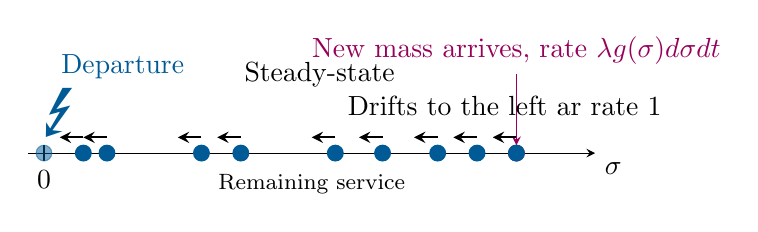
\begin{tikzpicture}    
			\draw [->] (-.2,0) -- node[midway,below,yshift=-1ex]{\footnotesize Remaining service} (7,0);
			\node [below right] at (7,0) {$\sigma$};
			\draw (0,.1) -- (0,-.1) node[below] {$0$};

			\uncover<2>{
				\draw [->,rojito] (6,1) node[above] {New mass arrives, rate $\lambda g(\sigma)d\sigma dt$} -- (6,.1);
				\draw [rojito, fill=rojito] (6,0) circle [radius=0.1];
			}
			\uncover<3>{
				\draw [azulcito, fill=azulcito] (6,0) circle [radius=0.1];
				\draw [thick,->] (6,.2) -- node[midway,above,yshift=1ex] {Drifts to the left ar rate $1$} ++(-.3,0);
			}
			\uncover<4>{
				\draw [azulcito, fill=azulcito, opacity = 0.5, fill opacity=0.5] (0,0) circle [radius=0.1];
				\node[azulcito] at (0.2,0.5) {\Huge\Lightning};
				\node[azulcito] at (1,1.1) {Departure};
			}
			\uncover<5->{
				\foreach \x in {.5,.8,2,2.5,3.7,4.3,5,5.5} {
					\draw [azulcito, fill=azulcito] (\x,0) circle [radius=0.1];
					\draw<5> [thick,->] (\x,.2) --  ++(-.3,0);
				}
				\node at (3.5,1) {Steady-state};
			}

			
		\end{tikzpicture}
	\end{center}
	\vfill
	\uncover<6->{
		\alert{State-descriptor:}
		\begin{equation*}
			\Phi_t = \sum_i \delta_{\sigma_i(t)}
		\end{equation*}
		a Point-process on the positive half-line.
	}
\end{frame}

\begin{frame}{M/G/$\infty$, steady state}
	
	\begin{itemize}
		\item $\Phi_t$ is a measure-valued Markov process.
		\item Its dynamics can be characterized through its generator.
		\item In steady state:
		\begin{equation*}
			\Phi \sim \textrm{Poisson Process with mean measure } \mu(d\sigma) = \lambda \bar{G}(\sigma)d\sigma
		\end{equation*}
		where $\bar{G}$ is the CCDF of $S$.
	\end{itemize}

	\pause
	\vfill
	\alert{Interpretation:}

	\begin{itemize}
	 \item Write $\mu(d\sigma) = \rho \left[\frac{1}{E[S]}(1-G(\sigma))\right]d\sigma$, with $\rho = \lambda E[S]$.
	 \item Then $\left[\frac{1}{E[S]}(1-G(\sigma))\right]d\sigma$ is the \emph{residual service time distribution} associated to $G$.
	 \item In steady-state, the total number of customers $\sim \textrm{Poisson}(\rho)$ and distributed in $\sigma$ as the residual lifetime distribution.
	\end{itemize}

\end{frame}

\begin{frame}{M/G/$\infty$, fluid approximation.}
	
	Suppose that we can replace $\Phi_t$ by a general measure $\mu_t$ with density $f(\sigma;t)$. 
	
	\begin{center}
		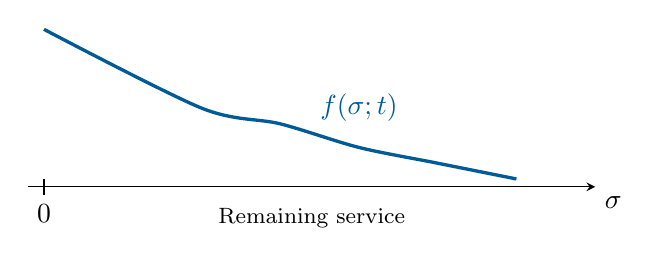
\begin{tikzpicture}    
			\draw [->] (-.2,0) -- node[midway,below,yshift=-1ex]{\footnotesize Remaining service} (7,0);
			\node [below right] at (7,0) {$\sigma$};
			\draw (0,.1) -- (0,-.1) node[below] {$0$};

			\draw [azulcito, very thick] plot [smooth] coordinates {(0,2) (2,1) (3,.8) (4,.5) (5,.3) (6,.1)};
			\node[azulcito] at (4,1) {$f(\sigma;t)$};
		\end{tikzpicture}
	\end{center}
	\begin{itemize}
		\item Mass is transported to the left at rate $1$.
		\item New mass arrives at $\sigma$ with intensity $\lambda g(\sigma)d\sigma dt$.
	\end{itemize}
\vfill
	We can combine this in the following \alert{transport equation}:
	\begin{equation*}
		\frac{\partial f}{\partial t} = \frac{\partial f}{\partial \sigma} + \lambda g(\sigma).
	\end{equation*}

\end{frame}

\begin{frame}{M/G/$\infty$, fluid approximation.}

	Imposing equilibrium and the boundary condition $f(\sigma)\to 0$ as $\sigma\to\infty$ we get:
	\begin{equation*}
		\frac{\partial f}{\partial \sigma} + \lambda g(\sigma) = 0 \Longrightarrow f(\sigma) = \lambda \int_\sigma^{\infty} g(u)\, du = \lambda \bar{G}(\sigma),
	\end{equation*}
	so the fluid approximation recovers the mean measure of $\Phi$.

	\pause\vfill
	\begin{itemize}
		\item This is a deterministic measure, with total mass $\rho$... 
		\item ...distributed in the real line as the residual service distribution.
		\item Serves as an approximation of $\Phi$ in a large scale system ($\lambda\to\infty$).
	\end{itemize}
\end{frame}

\begin{frame}{M/G/$\infty$: take two}{Attained service state descriptor}

	Here is another approach to model the same system \cite{kangramanan2010fluid}:
	\vfill
	\begin{center}
		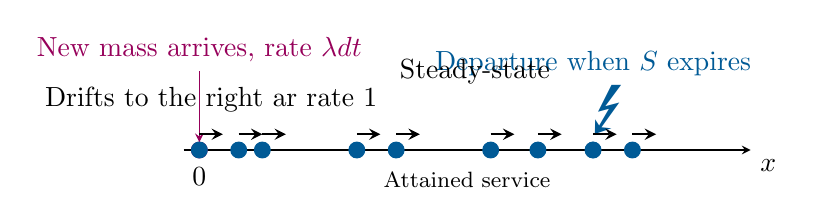
\begin{tikzpicture}    
			\draw [->] (-.2,0) -- node[midway,below,yshift=-1ex]{\footnotesize Attained service} (7,0);
			\node [below right] at (7,0) {$x$};
			\draw (0,.1) -- (0,-.1) node[below] {$0$};

			\uncover<2>{
				\draw [->,rojito] (0,1) node[above] {New mass arrives, rate $\lambda dt$} -- (0,.1);
				\draw [rojito, fill=rojito] (0,0) circle [radius=0.1];
			}
			\uncover<3>{
				\draw [azulcito, fill=azulcito] (0,0) circle [radius=0.1];
				\draw [thick,->] (0,.2) -- node[midway,above,yshift=1ex] {Drifts to the right ar rate $1$} ++(.3,0);
			}
			\uncover<4>{
				\draw [azulcito, fill=azulcito, opacity = 0.5, fill opacity=0.5] (5,0) circle [radius=0.1];
				\node[azulcito] at (5.2,0.5) {\Huge\Lightning};
				\node[azulcito] at (5,1.1) {Departure when $S$ expires};
			}
			\uncover<5->{
				\foreach \x in {.5,.8,2,2.5,3.7,4.3,5,5.5} {
					\draw [azulcito, fill=azulcito] (\x,0) circle [radius=0.1];
					\draw<5> [thick,->] (\x,.2) --  ++(.3,0);
				}
				\node at (3.5,1) {Steady-state};
			}

			
		\end{tikzpicture}
	\end{center}
	\vfill
	\uncover<6->{
		\alert{State-descriptor:}
		\begin{equation*}
			\tilde{\Phi}_t = \sum_i \delta_{x_i(t)}
		\end{equation*}
		a Point-process on the positive half-line, where $x_i(t)$ is the elapsed time in the system
	}

\end{frame}

\begin{frame}{M/G/$\infty$, take two}{Steady-state}
	
	$\tilde\Phi_t$ is a measure-valued Markov process.

	\begin{itemize}
		\item Mass always arrive at $0$ with rate $\lambda dt$.
		\item Transports to the right at rate $1$.
		\item Leaves the system at rate $h(x)$, the \alert{hazard rate function}:
		\begin{equation*}
			h(x) = \lim_{dt\to 0} P(S\in[x,x+dt]\mid S>x) = \frac{g(x)}{\bar{G}(x)} = -\frac{\partial}{\partial x} \log \bar{G}(x).
		\end{equation*}
	\end{itemize}

	\pause
	\vfill
	\alert{Steady-state:}
		\begin{equation*}
			\tilde\Phi \sim \textrm{Poisson Process with mean measure } \nu(dx) = \lambda \bar{G}(x)dx
		\end{equation*}
	
	
	\vfill

	So the reversed representation has the same distribution, because in a random point in time the elapsed service and the remaining service have the same distribution.

\end{frame}


\begin{frame}{M/G/$\infty$: take two}{Fluid approximation.}
	
	Suppose that we can replace $\tilde\Phi_t$ by a general measure $\nu_t$ with density $\tilde f(x;t)$. 
	
	\begin{center}
		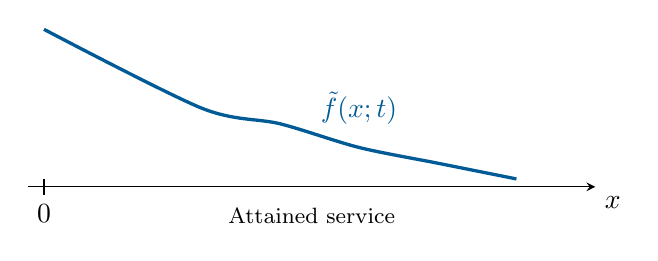
\begin{tikzpicture}    
			\draw [->] (-.2,0) -- node[midway,below,yshift=-1ex]{\footnotesize Attained service} (7,0);
			\node [below right] at (7,0) {$x$};
			\draw (0,.1) -- (0,-.1) node[below] {$0$};

			\draw [azulcito, very thick] plot [smooth] coordinates {(0,2) (2,1) (3,.8) (4,.5) (5,.3) (6,.1)};
			\node[azulcito] at (4,1) {$\tilde f(x;t)$};
		\end{tikzpicture}
	\end{center}
\vfill
\pause
The corresponding transport equation is (informally):
	\begin{equation*}
		\frac{\partial \tilde f}{\partial t} = -\frac{\partial \tilde f}{\partial x} - h(x)\tilde{f} + \lambda \delta_0.
	\end{equation*}
\end{frame}

\begin{frame}{M/G/$\infty$: take two}{Fluid equilibrium.}
	
Imposing equilibrium we get:
	\begin{equation*}
		\frac{\partial \tilde f}{\partial x} = - h(x)\tilde{f} + \lambda \delta_0.
	\end{equation*}

Solving (in a distribution sense) with the boundary condition $\tilde f (\infty) = 0$ we get:
	\begin{equation*}
		\tilde{f}(x) = \lambda e^{-\int_0^x h(u)du}.
	\end{equation*}

But by definition $\int_0^x h(u) du = -\log \bar{G}(x)$, and thus:
	\begin{equation*}
		\tilde{f}(x) = \lambda \bar{G}(x)
	\end{equation*}

So the transport fluid equation recovers again the mean measure of the steady-state.

\end{frame}

\begin{frame}{Lessons learned}

	\begin{myitem}
		\item We can model $M/G$ systems by using two state descriptors:
			\begin{itemize}
				\item The remaining service $\Phi$.
				\item The attained service $\tilde\Phi$.
			\end{itemize}
		\item Both admit reasonable fluid approximations, which correspond to transport equations.
		\item In fact this has been used in the literature to model abandonments (since they operate as $M/G/\infty$ systems in some sense).
	\end{myitem}
	\pause \vfill
	\alert{Question:} can we do more using this machinery of measure-valued processes?
\end{frame}

\section{Partial service queues and Earliest-Deadline-First}

\begin{frame}{Partial service queues}{Setting}

	Consider an $M/G/C$ system where:
	\begin{columns}
		\begin{column}{0.5\textwidth}
			\begin{itemize}
			\item Tasks arrive as a Poisson process of intensity $\lambda$.
			\item<2-> Each task $i$ has two characteristics (marks):
			\begin{itemize}
				\item $S_i$: service time (at rate $1$).
				\item $T_i$: sojourn time or deadline.
			\end{itemize}
			\item<3-> $(S_i,T_i)$ are independent across jobs.
			\item<3-> Follow a common distribution $G(\sigma,\tau)$, possibly correlated.
			\end{itemize} 
		\end{column}
		\begin{column}{0.5\textwidth}

			\begin{tikzpicture}
				\node (arrival) at (0,0) {$\lambda$};
				\node [right of=arrival] (queuel) {};
				\draw[->] (arrival) -- (queuel);
				\draw[thick] (queuel)++(0,.6) --node[midway,above] {Queue} ++(3,0) -- ++(0,-1.2) -- ++(-3,0);

				\foreach \x in {2,2.4,2.8,3.2,3.6} {
					\fill[rojito,thick, fill=rojito!70!white] (\x,.5) rectangle ++(.3,-1);
				}
				\foreach \y in {2,1,0,-1,-2} {
					\draw[azulcito, thick, fill=azulcito!70!white] (5,\y) circle [radius=.4];
				}
				\node[above] at (5,2.5) {$C$ servers};

				\draw<2->[thick,rojito] (2.5,-.75) rectangle ++(1,-1.6);
				\node<2-> at (3,-1.2) {
\includegraphics[width=.5cm]{figuras/battery_mid.png}};
				\node<2-> at (3,-2) {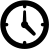
\includegraphics[width=.5cm]{figuras/clock.png}};

				\draw<2->[rojito,thick,->] (2.15,-.5) -- (2.15,-1.6) -- (2.5,-1.6);
			\end{tikzpicture}

		\end{column}
	\end{columns}
\end{frame}

\begin{frame}{Partial service queues}{Definition}

	\begin{block}{Partial service queue}
		Customers depart whenever $S_i$ is attained or the timer $T_i$ expires.
	\end{block}
	\vfill

	\pause
	\begin{myitem}
		\item In particular, they may leave \alert{during service}.

		\item Key performance metrics:
		\begin{myitem}[1em]
			\item \alert{$S_a$}: amount of service \alert{attained}.
			\item Equivalently, \alert{$S_r$}$:=S-S_a$, amount of service \alert{reneged}. 
		\end{myitem}

		\pause

		\item \alert{Problem:} we have to keep track of remaining service and deadlines simultaneously!
	\end{myitem}
\end{frame}


\begin{frame}{System load}

	\begin{myitem}
		
	\item Before proceeding, it is useful to define the \alert{system load}:

	\begin{equation*}
		\rho:= \lambda E[\min\{S,T\}].
	\end{equation*}

	\pause

	\item \alert{Interpretation:} the mean number of customers on a system with $C=\infty$.

	\item What we expect in a large scale fluid model:
	
	\begin{itemize}
	 \item If $\rho<C$ (underload), all tasks can be served, $S_a = \min\{S,T\}$.
	 \item If $\rho>C$ (overload), demand \emph{curtailing} will occur. How? It depends on the policy...
	\end{itemize}

	\end{myitem}


\end{frame}

\begin{frame}{System evolution}{Remaining service times}

	\begin{columns}
	\begin{column}{0.45\textwidth}
		  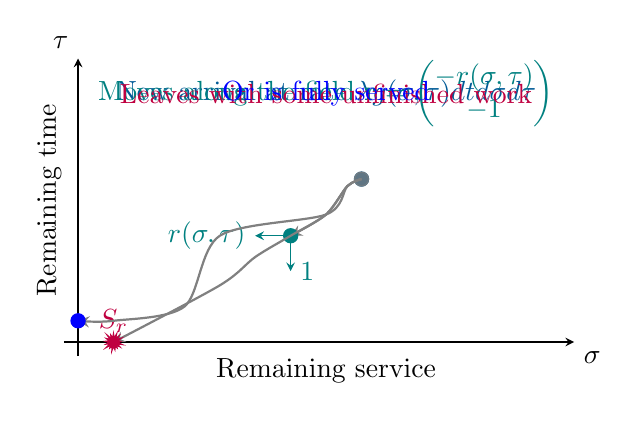
\begin{tikzpicture}[scale=0.9]
    
			\draw [->] (-.2,0) -- (7,0);
			\node [below right] at (7,0) {$\sigma$};
			\draw [->] (0,-.2) -- (0,4);
			\node [above left] at (0,4) {$\tau$};
			
			\node [below] at (3.5,-.1) {Remaining service};
			\node [rotate=90, left, anchor=south] at (-.1,2) {Remaining time};
			
			%	\draw [thick,gray,->] (4,2.3) -- ++(0,-.4);
			\draw<2> [azulcito, fill=azulcito] (4,2.3) circle [radius=0.1];
			\node<2> [azulcito] at (3.5,3.5) {New arrival at rate $\lambda g(\sigma,\tau)dtd\sigma d\tau$};

			\draw<3> [thick,gray,->] plot[smooth] coordinates {(4,2.3) (3.8,2.2) (3.5,1.8) (3,1.5)}; 
			\draw<3> [gray, fill=gray, opacity=0.5] (4,2.3) circle [radius=0.1];
			\draw<3> [teal, fill=teal] (3,1.5) circle [radius=0.1];
			\draw<3> [teal, fill=teal,->] (3,1.5) -- (2.5,1.5) node[left]{$r(\sigma,\tau)$};
			\draw<3> [teal, fill=teal,->] (3,1.5) -- (3,1) node[right]{$1$};
			\node<3> [teal] at (3.5,3.5) {Moves along the field $\mathbf{r} = \begin{pmatrix}
			-r(\sigma,\tau) \\ -1
			\end{pmatrix}$};

			\draw<4> [thick,gray,->] plot[smooth] coordinates {(4,2.3) (3.8,2.2) (3.5,1.8) (3,1.5) (2.5,1.2) (2,.8) (.5,0)}; 
			\draw<4-5> [gray, fill=gray, opacity=0.5] (4,2.3) circle [radius=0.1];
			\node<4>[purple, fill=purple, starburst, inner sep=1.5pt,/pgf/starburst point height=3] at (.5,0) {};
			\node<4>[purple,above] at (.5,0) {$S_r$};
			\node<4> [purple] at (3.5,3.5) {Leaves with some unfinished work};

			\draw<5> [thick,gray,->] plot[smooth] coordinates {(4,2.3) (3.8,2.2) (3.5,1.8) (2,1.5) (1.5,.5) (.5,.3) (0,.3)}; 
			\draw<5> [blue, fill=blue] (0,.3) circle [radius=0.1];
			\node<5> [blue] at (3.5,3.5) {Or is fully served};

		\end{tikzpicture}

	\end{column}
	\begin{column}{0.55\textwidth}
		\begin{itemize}
			\item<1-> Consider the remaining time space.
			\item<3-> \alert{Policy} defines how tasks are served.
			\item<3-> May depend on any combination of $(\sigma,\tau)$.
			\item<5-> State descriptor:
			 \begin{equation*}
				\Phi_t = \sum_i \delta_{\left(\sigma_i(t),\tau_i(t)\right)}
			 \end{equation*}
		\end{itemize}
	\end{column}
	\end{columns}

\end{frame}

\begin{frame}{Example: Earliest-deadline-first}

	\begin{columns}
		\begin{column}{0.45\textwidth}
		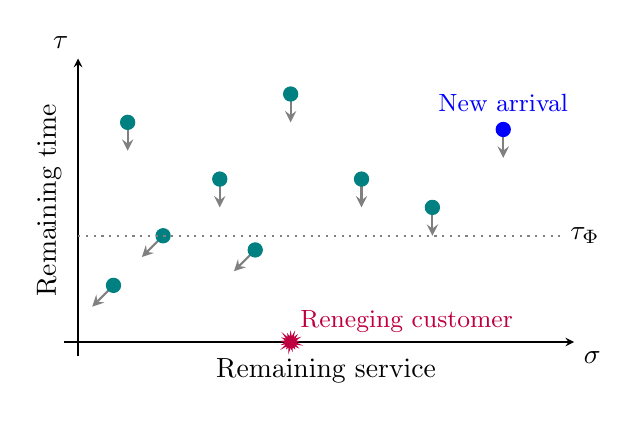
\begin{tikzpicture}[scale=0.9]
				
			\draw [->] (-.2,0) -- (7,0);
			\node [below right] at (7,0) {$\sigma$};
			\draw [->] (0,-.2) -- (0,4);
			\node [above left] at (0,4) {$\tau$};
			
			\node [below] at (3.5,-.1) {Remaining service};
			\node [rotate=90, left, anchor=south] at (-.1,2) {Remaining time};
			
			\draw [thick,gray,->] (.5,.8) -- ++(-.3,-.3);
			\draw [thick,gray,->] (.7,3.1) -- ++(0,-.4);
			\draw [thick,gray,->] (1.2,1.5) -- ++(-.3,-.3);
			\draw [thick,gray,->] (2,2.3) -- ++(0,-.4);
			\draw [thick,gray,->] (2.5,1.3) -- ++(-.3,-.3);
			\draw [thick,gray,->] (3,3.5) -- ++(0,-.4);
			\draw [thick,gray,->] (4,2.3) -- ++(0,-.4);
			\draw [thick,gray,->] (5,1.9) -- ++(0,-.4);
			\draw [thick,gray,->] (6,3) -- ++(0,-.4);

			\draw [teal, fill=teal] (.5,.8) circle [radius=0.1];
			\draw [teal, fill=teal] (.7,3.1) circle [radius=0.1];
			\draw [teal, fill=teal] (1.2,1.5) circle [radius=0.1];
			\draw [teal, fill=teal]  (2,2.3) circle [radius=0.1];
			\draw [teal, fill=teal] (2.5,1.3) circle [radius=0.1];
			\draw [teal, fill=teal] (3,3.5) circle [radius=0.1];
			\draw [teal, fill=teal] (4,2.3) circle [radius=0.1];
			\draw [teal, fill=teal] (5,1.9) circle [radius=0.1];
			\draw [blue, fill=blue] (6,3) circle [radius=0.1] node[above, yshift=3pt] {\small New arrival};

			%reneging departure
			%\draw [purple, fill=purple!20!white] (3,0) circle [radius=0.1] node[above, anchor=south west] {\small Reneging customer};
			\node[purple, fill=purple, starburst, inner sep=1.5pt,/pgf/starburst point height=3] at (3,0) {};
			\node[purple, anchor=south west] at (3,0){ \small Reneging customer};

			\draw [gray, dotted, thick] (0,1.5) -- (6.8,1.5) node[black, right] {$\tau_\Phi$};

		\end{tikzpicture}
	\end{column}
	\begin{column}{0.55\textwidth}
		\begin{itemize}
			\item Serve the $C$ most urgent customers.
			\item Corresponds to taking:
				\begin{equation*}
					r_\Phi(\sigma,\tau) = \mathbf{1}_{\{\tau\leqslant\tau_\Phi\}} 
				\end{equation*}
				with
				\begin{equation*} 
					\tau_\Phi := \sup\{\tau \geqslant 0: \Phi(\mathbb{R}_{+} \times (0, \tau]) < C\}. 	
				\end{equation*} 
		\end{itemize}
	\end{column}
\end{columns}
\end{frame}


\begin{frame}{Fluid model dynamics}
	\begin{itemize}
		\item Replace $\Phi_t$ by a (fluid) measure $\mu_t$.
		\item Now mass drifts along the field:
			\begin{equation*}
				\mathbf{r}_\mu(\sigma,\tau) = \begin{pmatrix}
				-r_\mu(\sigma,\tau) \\
				-1
				\end{pmatrix}
 			\end{equation*}
		\item With $r_\mu$ satisfying:
		\begin{gather*}
			0\leqslant r_{\mu} \leqslant 1 \\
			\iint r_\mu(\sigma,\tau) \mu(d\sigma,d\tau) \leqslant \min\{\mu(\R^2_{++}),C\}.
		\end{gather*} 
	\end{itemize}
\end{frame}

\begin{frame}{Fluid model dynamics}{Weak formulation}

	We will describe these dynamics in terms of the projections 
\begin{equation*}
	\brackets{\phi}{\mu} := \iint \phi(\sigma,\tau) \, \mu(d\sigma,d\tau)
\end{equation*}
of the state measure with  respect to a test function $\phi:\R^2_{++}\to\R$, with continuous derivatives and compact support, i.e. $\phi \in \mathcal{C}^1_c(\R^2_{++})$.  

\vfill

We have:
	\begin{equation*}
	\brackets{\phi}{\mu_{t+dt}} = \iint \phi(\sigma-r_{\mu_t}dt,\tau-dt) \, \mu_{t}(d\sigma,d\tau) + \lambda dt \iint \phi(\sigma,\tau)g(\sigma,\tau)\, d\sigma d\tau + o(dt).
\end{equation*}

\end{frame}

\begin{frame}{Fluid model dynamics}{Weak formulation}

	\begin{align*}
	\frac{\partial}{\partial t}\brackets{\phi}{\mu_{t}} =& \lim_{dt\to 0} \iint \frac{1}{dt} \left[\phi(\sigma-r_{\mu_t}dt,\tau-dt) - \phi(\sigma,\tau)\right] \mu_{t}(d\sigma,d\tau) \\ 
	&+ \lambda \iint \phi(\sigma,\tau)g(\sigma,\tau) d\sigma d\tau\\
=& - \iint \left[r_{\mu_t}(\sigma,\tau) \phi_\sigma (\sigma,\tau) + \phi_\tau(\sigma,\tau)\right]\mu_t(d\sigma,d\tau) + \lambda \iint \phi(\sigma,\tau)g(\sigma,\tau) d\sigma d\tau,
\end{align*}

\end{frame}

\begin{frame}{Fluid model dynamics}{Weak formulation}

	Equivalently:

\begin{align*}
	\brackets{\phi}{\mu_t} = \brackets{\phi}{\mu_0} + \int_0^t &\left[- \iint \left[r_{\mu_s}(\sigma,\tau) \phi_\sigma (\sigma,\tau) + \phi_\tau(\sigma,\tau)\right]\mu_t(d\sigma,d\tau)\right.\\
	& \left. + \lambda \iint \phi(\sigma,\tau)g(\sigma,\tau)\, d\sigma d\tau \right]ds,
\end{align*}
for any $\phi \in \mathcal{C}^1_c(\R^2_{++})$.

\pause
\vfill

Looks daunting, but is not that bad...

\end{frame}

\begin{frame}{Fluid model dynamics}{Transport PDE}

	If $\mu_t$ admits a density $f(\sigma,\tau;t)$ with respect to the Lebesgue measure, it corresponds to:

	\begin{equation*}
		\frac{\partial f}{\partial t} + \nabla \cdot\left[\mathbf{r}_{\mu_t} f\right] = \lambda g
	\end{equation*}
	a transport equation.

	\pause

	\vfill

	\alert{Example: EDF}

	\begin{equation*}
		\frac{\partial f}{\partial t} = \frac{\partial f}{\partial \sigma}\ind{\tau<\tau_{\mu_t}} + \frac{\partial f}{\partial \tau} +\lambda g
	\end{equation*}

\end{frame}

\begin{frame}{EDF Fluid model equilibrium}

	Imposing equilibrium we get:

	\begin{myitem}
		\item $\tau_{\mu^*}=\tau^*$ becomes a constant.
		\item The measure $\mu^*$ must satisfy:
			 \begin{equation*}
				\frac{\partial f}{\partial \sigma}\ind{\tau<\tau^*}  + \frac{\partial f}{\partial \tau} +\lambda g = 0.
			\end{equation*}
		\item Linear PDE that can be easily solved by the method of characteristics.
	\end{myitem}


\end{frame}

\begin{frame}{Solving the EDF transport equation}

	\begin{center}
	
	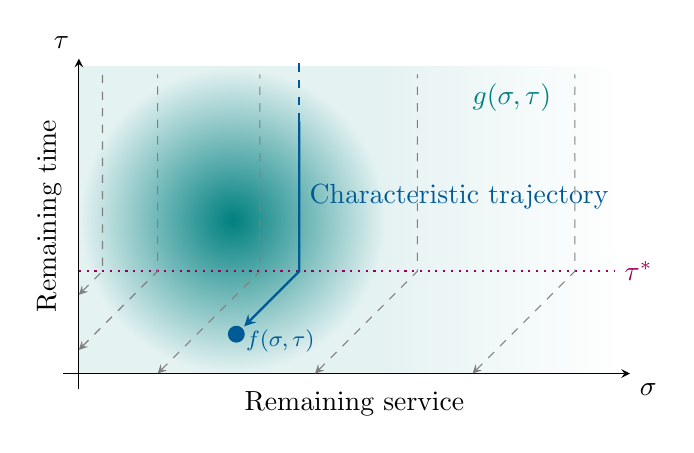
\begin{tikzpicture}
  
	\shade[inner color=teal,outer color=teal!10!white] (0,0) rectangle (3.9,3.9);
	\shade[left color=teal!10!white,right color=white] (3.9,0) rectangle (6.9,3.9);

  \node[teal] at (5.5,3.5) {$g(\sigma,\tau)$};
  \draw [->] (-.2,0) -- (7,0);
  \node [below right] at (7,0) {$\sigma$};
  \draw [->] (0,-.2) -- (0,4);
  \node [above left] at (0,4) {$\tau$};
  
  \node [below] at (3.5,-.1) {Remaining service};
  \node [rotate=90, left, anchor=south] at (-.1,2) {Remaining time};
  
%	\draw [thick,gray,->] (4,2.3) -- ++(0,-.4);
  \draw [rojito, dotted, thick] (0,1.3) -- (6.8,1.3) node[right] {$\tau^*$};
  \draw [azulcito, fill=azulcito] (2,.5) circle [radius=0.1] node[below right, yshift=5pt] {\footnotesize $f(\sigma,\tau)$};

  \draw [azulcito,thick,<-] (2.1,.6) -- (2.8,1.3) -- node[midway, anchor=west] {Characteristic trajectory} (2.8,3.2);
  \draw [azulcito,thick,dashed] (2.8,3.2) -- (2.8,4);

  \draw [gray,dashed,<-] (0,1) -- (.3,1.3) -- (.3,3.8);
  \draw [gray,dashed,<-] (0,.3) -- (1,1.3) -- (1,3.8);
  \draw [gray,dashed,<-] (1,0) -- (2.3,1.3) -- (2.3,3.8);
  \draw [gray,dashed,<-] (3,0) -- (4.3,1.3) -- (4.3,3.8);
  \draw [gray,dashed,<-] (5,0) -- (6.3,1.3) -- (6.3,3.8);

  \end{tikzpicture}
	\end{center}

\end{frame}

\begin{frame}{EDF in overload}{Fluid model equilibrium}

	\begin{theorem}
    Assume that $\rho > C$ and the equation
	\begin{equation*}
		\lambda E[\min\{S,T,\tau^*\}] = C
	\end{equation*}
    has a unique solution $\tau^* > 0$. Consider the measure $\mu^*$ given by the following density:
    \begin{equation*}
		f(\sigma, \tau) = \lambda\left[\int_0^{\left(\tau^* - \tau\right)^+} g(\sigma + u, \tau + u)du + \int_{\left(\tau^* - \tau\right)^+}^\infty g\left(\sigma + \left(\tau^* - \tau\right)^+, \tau + u\right)du\right]. 
	\end{equation*}

	This measure is a fluid equilibrium for the EDF policy, and 
	\begin{equation*}
	\tau^* = \sup \left\{\tau \geq 0:\mu^*(\R_{++} \times (0, \tau]) \leq C\right\}.
	\end{equation*}
	\end{theorem}

\end{frame}

\begin{frame}{EDF performance in equilibrium}
	
	\begin{columns}
		\begin{column}{0.5\textwidth}
		\begin{itemize}
		\item Let us compute the rate at which work is \alert{reneged}.
		
		\item Compute the rate at which mass exits with $S_r < \sigma_0$.
		
		\end{itemize}
		\end{column}
		\begin{column}{0.5\textwidth}
			\begin{tikzpicture}[scale=0.7]
				
			\draw [->] (-.2,0) -- (7,0);
			\node [below right] at (7,0) {$\sigma$};
			\draw [->] (0,-.2) -- (0,4);
			\node [above left] at (0,4) {$\tau$};
			
%			\node [below] at (3.5,-.1) {Remaining service};
%			\node [rotate=90, left, anchor=south] at (-.1,2) { Remaining time};

			\draw [gray, dotted, thick] (0,1.5) -- (6.8,1.5) node[black, right] {$\tau_\Phi$};

			\draw[very thick,rojito] (0,1.5) -- (0,0) -- (2,0);
			\draw[very thick,rojito] (2,.2) -- (2,-.2) node[below]{$\sigma_0$};

			\draw[thick,gray] (2,0) -- (3.5,1.5) -- (3.5,4);

			\draw[thick,gray,->] (1.75,3) -- ++(0,-.9);
			\draw[thick,gray,->] (1.5,1) -- ++(-.6,-.6);

			\end{tikzpicture}
		\end{column}
	\end{columns}

	\begin{proposition}
    \begin{equation*}
        \int_0^{\tau^*} f(0, \tau)d\tau + \int_0^{\sigma_0} f(\sigma, 0)d\sigma = \lambda P\left(S - \min\left\{S, T, \tau^*\right\} < \sigma_0\right).
    \end{equation*}

	\smallskip
	i.e. $S_a = S-S_r = \min\{S,T,\tau^*\}$.
	\end{proposition}
\end{frame}


\section{Deadline-oblivious policies}

\begin{frame}{What if we do not know the deadlines?}

	\begin{myitem}
	\item Deadlines are often hard to estimate in practice.
	\item Moreover, tasks may under-report their deadline to get priority!
	\item What about \alert{deadline-oblivious} policies?
	\begin{itemize}
		\item Can we model them?
		\item What is their performance?
	\end{itemize}
	\end{myitem}
	
	\pause
	\vfill
	\alert{Problem:} we need a new state-space...
\end{frame}


\begin{frame}{Attained service state descriptor}

	\begin{columns}
	\begin{column}{0.45\textwidth}
		  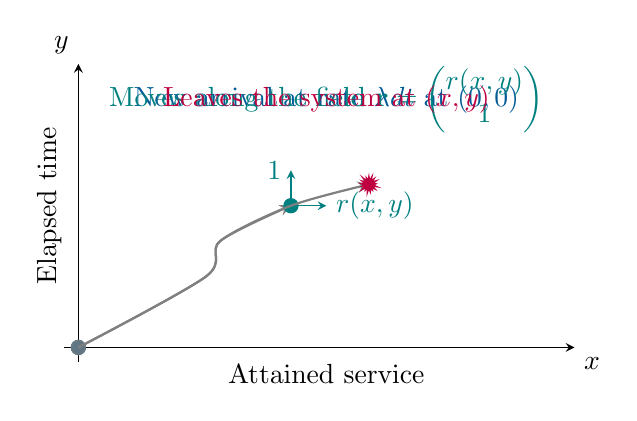
\begin{tikzpicture}[scale=0.9]
		
			\draw [->] (-.2,0) -- (7,0);
			\node [below right] at (7,0) {$x$};
			\draw [->] (0,-.2) -- (0,4);
			\node [above left] at (0,4) {$y$};
			
			\node [below] at (3.5,-.1) {Attained service};
			\node [rotate=90, left, anchor=south] at (-.1,2) {Elapsed time};

			\draw<2> [azulcito, fill=azulcito] (0,0) circle [radius=0.1];
			\node<2> [azulcito] at (3.5,3.5) {New arrival at rate $\lambda dt$ at $(0,0)$};

			\draw<3> [thick,gray,->] plot[smooth] coordinates {(0,0) (1.8,1) (2,1.5) (3,2)}; 
			\draw<3> [gray, fill=gray, opacity=0.5] (0,0) circle [radius=0.1];
			\draw<3> [teal, fill=teal] (3,2) circle [radius=0.1];
			\draw<3> [teal, fill=teal,->] (3,2) -- (3.5,2) node[right]{$r(x,y)$};
			\draw<3> [teal, fill=teal,->] (3,2) -- (3,2.5) node[left]{$1$};
			\node<3> [teal] at (3.5,3.5) {Moves along the field $\mathbf{r} = \begin{pmatrix}
			r(x,y) \\ 1
			\end{pmatrix}$};

			\draw<4-> [thick,gray,->] plot[smooth] coordinates {(0,0) (1.8,1) (2,1.5) (3,2) (4.1,2.3)}; 
			\draw<4-> [gray, fill=gray, opacity=0.5] (0,0) circle [radius=0.1];
			\node<4-> [purple, fill=purple, starburst, inner sep=1.5pt,/pgf/starburst point height=3] at (4.1,2.3) {};
			\node<4-> [purple] at (3.5,3.5) {Leaves the system at $(x,y)$};
			\end{tikzpicture}

	\end{column}
	\begin{column}{0.55\textwidth}
		\begin{itemize}
			\item<1-> Consider the elapsed time space.
			\item<3-> \alert{Policy} again defines how tasks are served.
			\item<3-> May depend on any combination of $(x,y)$.
			\item<5-> State descriptor:
			 \begin{equation*}
				\tilde\Phi_t = \sum_i \delta_{\left(x_i(t),y_i(t)\right)}
			 \end{equation*}
		\end{itemize}
	\end{column}
	\end{columns}

\end{frame}


\begin{frame}{Example: Least-Attained-Service policy}

	\begin{columns}
		\begin{column}{0.45\textwidth}
		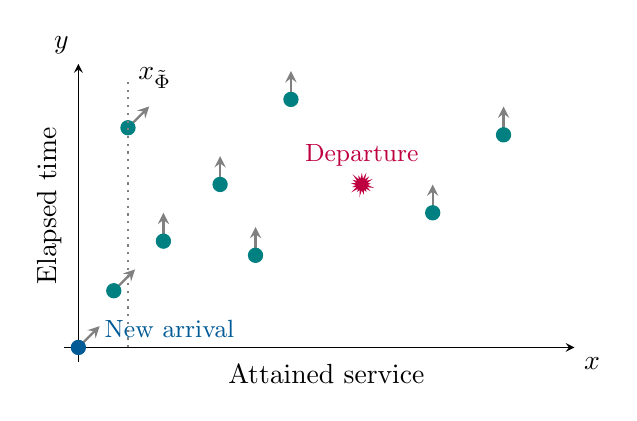
\begin{tikzpicture}[scale=0.9]
			\draw [->] (-.2,0) -- (7,0);
			\node [below right] at (7,0) {$x$};
			\draw [->] (0,-.2) -- (0,4);
			\node [above left] at (0,4) {$y$};
			
			\node [below] at (3.5,-.1) {Attained service};
			\node [rotate=90, left, anchor=south] at (-.1,2) {Elapsed time};
			
			\draw [thick,gray,->] (.5,.8) -- ++(.3,.3);
			\draw [thick,gray,->] (.7,3.1) -- ++(.3,.3);
			\draw [thick,gray,->] (1.2,1.5) -- ++(0,.4);
			\draw [thick,gray,->] (2,2.3) -- ++(0,.4);
			\draw [thick,gray,->] (2.5,1.3) -- ++(0,.4);
			\draw [thick,gray,->] (3,3.5) -- ++(0,.4);
			%\draw [thick,gray,->] (4,2.3) -- ++(.2,.4);
			\draw [thick,gray,->] (5,1.9) -- ++(0,.4);
			\draw [thick,gray,->] (6,3) -- ++(0,.4);

			\draw [teal, fill=teal] (.5,.8) circle [radius=0.1];
			\draw [teal, fill=teal] (.7,3.1) circle [radius=0.1];
			\draw [teal, fill=teal] (1.2,1.5) circle [radius=0.1];
			\draw [teal, fill=teal]  (2,2.3) circle [radius=0.1];
			\draw [teal, fill=teal] (2.5,1.3) circle [radius=0.1];
			\draw [teal, fill=teal] (3,3.5) circle [radius=0.1];
			%\draw [teal!50!white, fill=teal!50!white] (4,2.3) starburst  node[teal,above] {\footnotesize Departure};
			%\node[teal!50!white, fill=teal, starburst, inner sep=1.5pt,/pgf/starburst point height=3] at (4,2.3) {}; 
			%\node[teal,above, yshift=3pt] at (4,2.3) {\footnotesize Departure};
			
			\node[purple, fill=purple, starburst, inner sep=1.5pt,/pgf/starburst point height=3] at (4,2.3) {};
			\node[purple, above, yshift=3pt] at (4,2.3){ \small Departure};
			
			\draw [teal, fill=teal] (5,1.9) circle [radius=0.1];
			\draw [teal, fill=teal] (6,3) circle [radius=0.1];
			
			%new arrival

			\draw [thick,gray,->] (0,0) -- ++(.3,.3);
			\draw [azulcito, fill=azulcito] (0,0) circle [radius=0.1] node[anchor=south west, xshift=6pt] {\small New arrival};
			
			\draw [gray, dotted, thick] (.7,0) -- (.7,3.8) node[black, right] {$x_{\tilde{\Phi}}$};
	\end{tikzpicture}

	\end{column}
	\begin{column}{0.55\textwidth}
		\begin{itemize}
			\item Serve the $C$ least-served tasks.
			\item Corresponds to taking:
				\begin{equation*}
					r_{\tilde\Phi}(x,y) = \mathbf{1}_{\{x\leqslant x_{\tilde\Phi}\}} 
				\end{equation*}
				with
				\begin{equation*} 
					x_{\tilde\Phi} := \sup\{x: \tilde\Phi([0, x] \times \R_+) \leqslant C\}. 	
				\end{equation*} 
		\end{itemize}
	\end{column}
\end{columns}

\end{frame}


\begin{frame}{Example: Last-Come-First-Served policy}
  
	\begin{columns}
		\begin{column}{0.45\textwidth}
			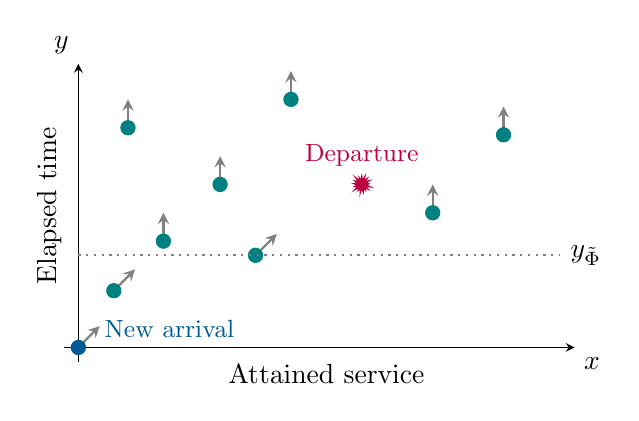
\begin{tikzpicture}[scale=0.9]
					
				\draw [->] (-.2,0) -- (7,0);
				\node [below right] at (7,0) {$x$};
				\draw [->] (0,-.2) -- (0,4);
				\node [above left] at (0,4) {$y$};
				
				\node [below] at (3.5,-.1) {Attained service};
				\node [rotate=90, left, anchor=south] at (-.1,2) {Elapsed time};
				
				\draw [thick,gray,->] (.5,.8) -- ++(.3,.3);
				\draw [thick,gray,->] (.7,3.1) -- ++(0,.4);
				\draw [thick,gray,->] (1.2,1.5) -- ++(0,.4);
				\draw [thick,gray,->] (2,2.3) -- ++(0,.4);
				\draw [thick,gray,->] (2.5,1.3) -- ++(.3,.3);
				\draw [thick,gray,->] (3,3.5) -- ++(0,.4);
				%\draw [thick,gray,->] (4,2.3) -- ++(.2,.4);
				\draw [thick,gray,->] (5,1.9) -- ++(0,.4);
				\draw [thick,gray,->] (6,3) -- ++(0,.4);

				\draw [teal, fill=teal] (.5,.8) circle [radius=0.1];
				\draw [teal, fill=teal] (.7,3.1) circle [radius=0.1];
				\draw [teal, fill=teal] (1.2,1.5) circle [radius=0.1];
				\draw [teal, fill=teal]  (2,2.3) circle [radius=0.1];
				\draw [teal, fill=teal] (2.5,1.3) circle [radius=0.1];
				\draw [teal, fill=teal] (3,3.5) circle [radius=0.1];
				%\draw [teal!50!white, fill=teal!50!white] (4,2.3) starburst  node[teal,above] {\footnotesize Departure};
				%\node[teal!50!white, fill=teal, starburst, inner sep=1.5pt,/pgf/starburst point height=3] at (4,2.3) {}; 
				%\node[teal,above, yshift=3pt] at (4,2.3) {\footnotesize Departure};
				\draw [teal, fill=teal] (5,1.9) circle [radius=0.1];
				\draw [teal, fill=teal] (6,3) circle [radius=0.1];
						
				\node[purple, fill=purple, starburst, inner sep=1.5pt,/pgf/starburst point height=3] at (4,2.3) {};
				\node[purple, above, yshift=3pt] at (4,2.3){ \small Departure};
				
				%new arrival

				\draw [thick,gray,->] (0,0) -- ++(.3,.3);
				\draw [azulcito, fill=azulcito] (0,0) circle [radius=0.1] node[anchor=south west, xshift=6pt] {\small New arrival};
				
				\draw [gray, dotted, thick] (0,1.3) -- (6.8,1.3) node[black, right] {$y_{\tilde{\Phi}}$};
				\end{tikzpicture}
		\end{column}
	\begin{column}{0.55\textwidth}
		\begin{itemize}
			\item Serve the $C$ more recent tasks.
			\item Corresponds to taking:
				\begin{equation*}
					r_{\tilde\Phi}(x,y) = \mathbf{1}_{\{y\leqslant y_{\tilde\Phi}\}} 
				\end{equation*}
				with
				\begin{equation*} 
					y_{\tilde\Phi} := \sup\{y: \tilde\Phi(\R_+\times [0, y]) \leqslant C\}
				\end{equation*} 
		\end{itemize}
	\end{column}
\end{columns}

\end{frame}

\begin{frame}{The hazard rate field}

	We have a new problem: what is the rate at which users \alert{leave} the system?

	\pause

	\vfill

	Let $\bar{G}(x,y) = P(S>x,T>y)$ and define:

	\begin{definition}[Hazard rate field]
		\begin{equation*}
			\mathbf{h}(x,y) = -\nabla \log \bar{G}(x,y)	\quad \text{i.e.}
		\end{equation*}
		\begin{itemize}
			\item $h^x (x,y) = P(S\in[x,x+dx],T>S \mid S>x,T>y)$
			\item $h^y (x,y) = P(T\in[y,y+dy],S>T \mid S>x,T>y)$
		\end{itemize}
	\end{definition}

	\vfill

	Interpretation: $\mathbf{h}$ stores the rate at which $\min\{S,T\}$ is attained due to $S$ or $T$ expiring.
\end{frame}

\begin{frame}{Fluid model dynamics}

	\begin{itemize}
		\item Replace $\tilde{\Phi}_t$ by a (fluid) measure $\nu_t$.
		\item Now mass arrives at $(0,0)$ at rate $\lambda$.
		\item Drifts along the field:
		 \begin{equation*}
			\mathbf{r}_\nu(x,y) = \begin{pmatrix}
				r_\nu (x,y) \\ 1
			\end{pmatrix}
		 \end{equation*}
		 \item With $r_\nu$ satisfying:
		 \begin{gather*}
			0\leqslant r_\nu \leqslant 1 \\
			\iint r_\nu(x,y) \nu(dx,dy) \leqslant \min\{\nu(\R^2_+),C\}.
		 \end{gather*}
	\end{itemize}
\end{frame}

\begin{frame}{Departure rate}

	Now we have to compute the departure rate $\eta_{\nu}(x,y)$:
	\begin{equation*}
		\eta_\nu(x,y) := \lim_{dt\to 0} \frac{1}{dt} P\left(\left\{S\in\left(x,x+r_{\tilde\Phi}dt\right)\right\}\cup \left\{T\in\left(y,y+dt\right)\right\}\mid S>x,T>y\right)
	\end{equation*}

	By the chain rule and some computations:
	\begin{gather*}
		\eta_{\nu}(x,y) =\frac{1}{\bar{G}(x,y)}\left[-\frac{\partial}{\partial x} \bar{G}(x,y) r_{\tilde\Phi}(x,y) - \frac{\partial}{\partial y} \bar{G}(x,y)\right]
	\end{gather*}
	\pause
	Therefore:
	\begin{equation*}
	\eta_{\nu}(x,y) = h^x(x,y)r_{\nu}(x,y)+h^y(x,y) = \mathbf{r}_{\nu}(x,y) \cdot \mathbf{h}(x,y).
	\end{equation*}

\end{frame}

\begin{frame}{Attained service transport equation}

	\begin{myitem}
		\item We now have all ingredients to formulate the dynamics of the system.
		\item The transport equation in the elapsed service space is (informally):
		\begin{equation*}
			\frac{\partial \bar f}{\partial t} + \nabla \cdot\left[\mathbf{r}_{\nu_t} \bar{f}\right] + [\mathbf{r}_{\nu_t}\cdot \mathbf{h}]\bar{f}= \lambda \delta_{(0,0)}.
		\end{equation*}
		where $\tilde{f}$ is the density of $\nu_t$.
		\pause
		\item The above equation must be treated in weak form:
		 \begin{itemize}
			\item To account for the impulse mass at $(0,0)$ driving the system.
			\item To allow solutions without a density as we shall see.
		 \end{itemize}
	\end{myitem}


\end{frame}


\begin{frame}{Last come first served}{Fluid equilibrium}

	Recall that LCFS can be modeled by:
	\begin{equation*}
		r_{\nu}(x, y) = \ind{y < y_\nu}
	\end{equation*}
	with
	\begin{equation*}
	y_\nu = \sup \left\{y \geq 0: \nu(\R_+ \times [0, y]) \leqslant C\right\}.
	\end{equation*}

	\pause
	\vfill
	Imposing equilibrium, $\nu^*$, $y^*$ fixed, we have to solve: 
	\begin{equation*}
		\nabla \cdot\left[\mathbf{r}_{\nu^*} \bar{f}\right] + [\mathbf{r}_{\nu^*}\cdot \mathbf{h}]\bar{f}= \lambda \delta_{(0,0)}.
	\end{equation*}

\end{frame}


\begin{frame}{Solving the transport equation}{Last come first served case}

	\begin{center}
	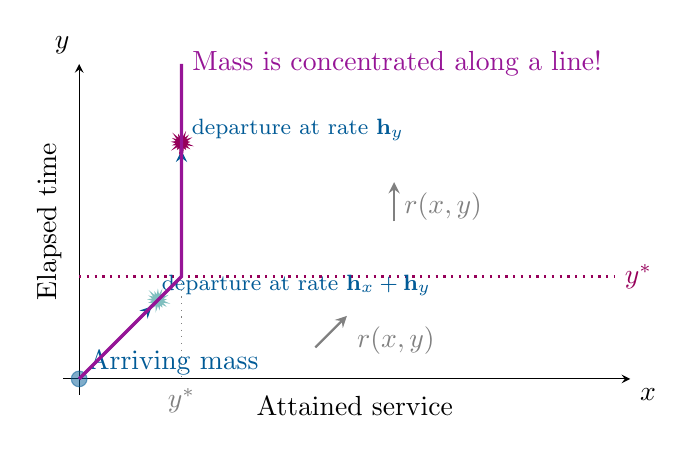
\begin{tikzpicture}
  
		\draw [->] (-.2,0) -- (7,0);
		\node [below right] at (7,0) {$x$};
		\draw [->] (0,-.2) -- (0,4);
		\node [above left] at (0,4) {$y$};
		
		\node [below] at (3.5,-.1) {Attained service};
		\node [rotate=90, left, anchor=south] at (-.1,2) {Elapsed time};

		\draw [gray,thick,->] (3,.4) -- (3.4,.8) node[below right] {$r(x,y)$};
		\draw [gray,thick, ->] (4,2) -- (4,2.5) node[below right] {$r(x,y)$};

		\draw [rojito, dotted, thick] (0,1.3) -- (6.8,1.3) node[right] {$y^*$};
		\draw [azulcito, fill=azulcito, opacity=0.5] (0,0) circle [radius=0.1]; 
		\node<1> [azulcito, anchor=west] at (0,.2) {Arriving mass};
		\draw<2> [azulcito,thick,->] (0,0) -- (.92,.92) node[above right] {\footnotesize departure at rate $\mathbf{h}_x+\mathbf{h}_y$};
		\node<2>[teal!50!white, fill=teal!50!white, starburst, inner sep=1.5pt,/pgf/starburst point height=3] at (1,1) {}; 
		\draw<3> [azulcito,thick,->] (0,0) -- (1.3,1.3) -- (1.3,2.9) node[above right] {\footnotesize departure at rate $\mathbf{h}_y$};
		\node<3>[rojito!50!white, fill=rojito, starburst, inner sep=1.5pt,/pgf/starburst point height=3] at (1.3,3) {}; 
		\draw<3>[gray, dotted] (1.3,1.3) -- (1.3,0) node[below] {$y^*$};

		\draw<4>[violetita, very thick] (0,0) -- (1.3,1.3) -- (1.3,4) node[right] {Mass is concentrated along a line!};
  \end{tikzpicture}

\end{center}

\end{frame}

\begin{frame}{Deadline-oblivious policies in overload}
	
	\begin{theorem}
    Assume that $\rho > C$ and the equation
	\begin{equation*}
		\lambda E[\min\{S,T,z^*\}] = C
	\end{equation*}
    has a unique solution $z^* > 0$. Consider the measure $\nu^*$ given by:
    \begin{equation*}
        \brackets{\phi}{\nu^*} = \lambda \left[\int_0^{z^*} \phi(u, u) \bar{G}(u, u)du + \int_{z^*}^\infty \phi\left(z^*, u\right)\bar{G}(z^*, u)du\right],
    \end{equation*}
    for all $\phi \in C_c(\R_+^2)$. Then this measure is the equilibrium measure for both the Least-Attained-Service and Last-Come-First-Served policies.
\end{theorem}

\end{frame}


\begin{frame}{LAS/LCFS performance in equilibrium}

	Compute the rate at which mass leaves the system with less than $x_0$ attained service:
	\begin{equation*}
		\iint_{[0,x_0]\times \R_+} \eta_{\nu^*} (x,y) \nu^*(dx,dy).
	\end{equation*}

	\pause

	\begin{proposition}
		Assume that $\rho > C$. Then
		\begin{equation*}
			\int_{[0,x_0]\times \R_+} \left[h^x(x, y) \ind{y < z^*} + h^y(x, y)\right]\nu^*(dx, dy) = \lambda P\left(\min\{S, T, z^*\} \leqslant x_0\right).
		\end{equation*}
	\end{proposition}
	
	So again the attained work is $S_a = \min\{S,T,z^*\}$!!

\end{frame}


\begin{frame}{Graphical explanation}

	\begin{center}
		
\tikzsetnextfilename{service_profile_edf}
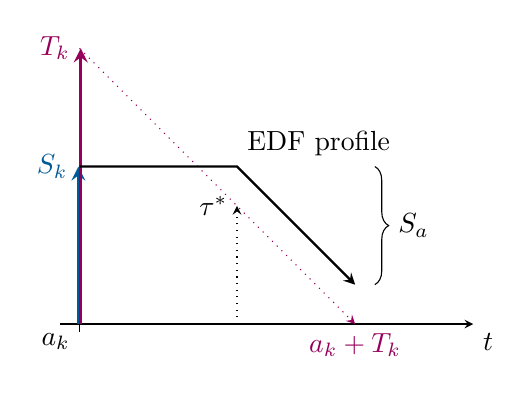
\begin{tikzpicture}[scale=0.5]
	\draw [->] (-.5,0) -- (10,0);
	\node [below right] at (10,0) {$t$};
	\draw [-] (0,-.2) -- (0,.2);
	\node [below left] at (0,0) {$a_k$};
	\draw [very thick,azulcito,->] (-.03,0) -- (-0.03,4) node  [left] {$S_k$};
	\draw [very thick,rojito,->] (.03,0) -- (0.03,7) node  [left] {$T_k$};
	\draw [dotted,rojito,->] (0,7) -- (7,0) node [below] {$a_k+T_k$};
	%\draw [dotted,azulcito,->] (0,4) -- (4,0) node [below] {$a_k+S_k$};
	%immediate scheduling
	\draw [black,thick,->] (0,4) -- (4,4) node[above right] {EDF profile}  -- (7,1);
	\draw [black,dotted,->] (4,0) -- (4,3) node [left] {$\tau^*$};

    \draw [decorate, decoration = {brace,mirror,amplitude=5pt}] (7.5,1) -- node[midway,right, xshift=5pt] {$S_a$} (7.5,4);

\end{tikzpicture}% \tikzsetnextfilename{service_profile_las_lcfs}
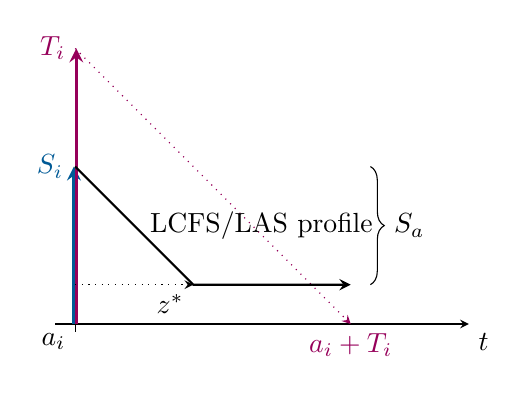
\begin{tikzpicture}[scale=0.5]
	
	\draw [->] (-.5,0) -- (10,0);
	\node [below right] at (10,0) {$t$};
	\draw [-] (0,-.2) -- (0,.2);
	\node [below left] at (0,0) {$a_i$};
	\draw [very thick,azulcito,->] (-.03,0) -- (-0.03,4) node  [left] {$S_i$};
	\draw [very thick,rojito,->] (.03,0) -- (0.03,7) node  [left] {$T_i$};
	\draw [dotted,rojito,->] (0,7) -- (7,0) node [below] {$a_i+T_i$};
	%\draw [dotted,azulcito,->] (0,4) -- (4,0) node [below] {$a_k+S_k$};
	%immediate scheduling
	\draw [black,thick,->] (0,4) -- node [midway, right,xshift=2pt] {LCFS/LAS profile} (3,1) -- (7,1);
	\draw [black,dotted,->] (0,1) -- (3,1) node [below left] {$z^*$};
	\draw [decorate, decoration = {brace,mirror,amplitude=5pt}] (7.5,1) -- node[midway,right, xshift=5pt] {$S_a$} (7.5,4);
\end{tikzpicture}%

	\end{center}

	\bigskip

	Since $\tau^* = x^* = y^* = z^*$, performance is the same in all three policies!!!
\end{frame}

\section{Simulations}

\begin{frame}{Simulations with correlated $S$ and $T$}
	\begin{itemize}
	\item We finally validate our fluid approximation by stochastic simulations
	\item In order to account for correlations, we take:
	 \begin{equation*}
    S = e^U \quad \text{and} \quad T = e^V \quad \text{with} \quad (U, V) \sim \mathcal{N}\left(\begin{pmatrix}
    0 \\ 0
    \end{pmatrix}, \begin{pmatrix}
    1 & 0.9 \\ 0.9 & 1
    \end{pmatrix}\right).
\end{equation*}
    \item In particular, the random variables $U$ and $V$ are correlated with normal distributions, and therefore $S$ and $T$ are correlated with log-normal distributions.
	\item In this case, $E[\min\{S,T\}] \approx 1.37$ can only be numerically estimated. 
	\item We choose $\lambda = 200$ and $C=100$, then $z^* \approx 0.593$.
	\end{itemize}
	

\end{frame}

\begin{frame}{State space snapshots}
    
	\begin{center}
	\tikzsetnextfilename{lognormal_edf_statespace}
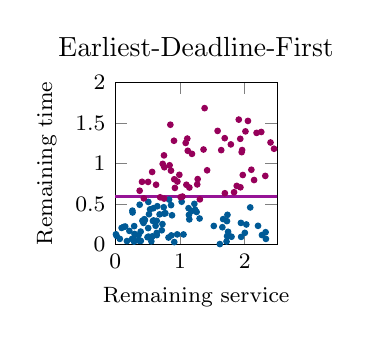
\begin{tikzpicture}

    \begin{axis}[
    title=Earliest-Deadline-First,
    width=0.3\textwidth,
    height=0.3\textwidth,
    xlabel={Remaining service},
    ylabel={Remaining time},
    xmin=0,xmax=2.5,
    ymin=0,ymax=2,
    legend style={font=\footnotesize},
    legend cell align=left,
    legend pos=north east,
    ]

    \addplot[color=azulcito, only marks, mark={*}, mark size=1.0 pt, mark options={color=azulcito, draw opacity={1.0}, fill=azulcito}]
        table[row sep={\\}]
        {
            \\
            35.72223187735489  0.1439930115625203  \\
            4.321021196872197  0.2650756470759983  \\
            15.28880256606086  0.0027984488087349213  \\
            3.5055678827782324  0.41489216015641883  \\
            7.391178965706386  0.1382091332974995  \\
            3.6508696834139753  0.41735205790430907  \\
            3.2460646075704145  0.1562147321473053  \\
            8.182791903533312  0.26068998744028615  \\
            5.536035127795618  0.45842588638343695  \\
            2.3231424488881074  0.15053890505421252  \\
            3.993018234280626  0.3454375610508773  \\
            2.025250500619911  0.24595340163079182  \\
            1.9418237336809625  0.2655164485675445  \\
            2.266622907393208  0.11541736582373785  \\
            4.645611208305086  0.09256456708230543  \\
            4.1027598740665585  0.192178130457207  \\
            2.0026028634997064  0.14254222024513252  \\
            3.944454647885422  0.47890304434561326  \\
            0.45967039058724746  0.3014674159290669  \\
            3.2403073052707767  0.12936808022543958  \\
            1.7279805057025421  0.10227941810835306  \\
            1.145054559193267  0.30857565193891645  \\
            0.9577900142511941  0.12338245816155838  \\
            1.223110254371425  0.5006922742939608  \\
            1.6554784171629584  0.21224325586151593  \\
            2.085557408376419  0.4567085799230455  \\
            3.305148962274741  0.05979639738926368  \\
            0.5389674595815077  0.4331116953970664  \\
            2.2060128327466684  0.22930602009785872  \\
            1.7198960641027927  0.035566412984707085  \\
            1.7437722649706298  0.15543445299947933  \\
            2.3276612829473096  0.06792825127644875  \\
            0.3962100964058868  0.0433553319865112  \\
            1.6673500353438062  0.31225121314584925  \\
            0.49898845518229784  0.08864062619026924  \\
            0.8329566897389348  0.5535038159808181  \\
            0.877665821571761  0.35984829115573547  \\
            0.9126455656378103  0.028481153806566795  \\
            0.5585699071837213  0.03774668242044754  \\
            0.5758480891027085  0.09995080004932788  \\
            1.6162794612703788  0.003922282516320763  \\
            0.1292399687292515  0.21557457112763245  \\
            0.7590603897267121  0.3797872599869052  \\
            0.6409290046291405  0.1411293529136799  \\
            1.523265625492039  0.22797726182862732  \\
            1.9451891114301678  0.09279375751069807  \\
            1.7262796084260819  0.28773938350266803  \\
            0.5152389339832235  0.09592822387146072  \\
            1.2349819960948656  0.4276031725956031  \\
            0.6414968261119827  0.2911555302187736  \\
            1.7968759797117637  0.09481545000744518  \\
            0.3612706503199621  0.11375932261284305  \\
            0.8674802552455381  0.11093954474868184  \\
            0.5829156249837795  0.2893506201322751  \\
            0.8238225320936134  0.08489344788214481  \\
            0.8631192878555354  0.4849036545654781  \\
            1.3038480316558336  0.31982740419953615  \\
            0.2769615523946991  0.06607744858823139  \\
            1.1790284221733283  0.4114193966833639  \\
            0.36653400115450396  0.04615683112484703  \\
            0.6860549215479166  0.370965807898024  \\
            0.0209855101330374  0.10701495129728045  \\
            0.5928009971982089  0.2960147272361908  \\
            1.1388304933437319  0.36421682855812776  \\
            0.6426544353194914  0.11437897231803618  \\
            1.7338805332296645  0.36499270578477194  \\
            0.6243474813319214  0.22979808841353844  \\
            0.15516661451656377  0.22084018234993152  \\
            0.591483241538773  0.44739495801350415  \\
            0.1816272438022467  0.041034399737455374  \\
            4.083888479967856  0.5487982884472942  \\
            1.0268634931319434  0.5272908086291181  \\
            1.0554025165449317  0.12290551199095037  \\
            0.28278663124692427  0.07121890040427559  \\
            0.012241923942466093  0.12493480100986434  \\
            0.6506339856719032  0.4715643121353139  \\
            0.7194480759565978  0.17456723701054955  \\
            0.39365233347705963  0.15823540956387205  \\
            0.7756757054212384  0.3853918743083824  \\
            0.7298617139580432  0.250703225068996  \\
            0.21942252300454312  0.16701853491734653  \\
            0.2917684874262658  0.03446662171902659  \\
            0.4368999160194622  0.2650632236637094  \\
            0.5101385565847241  0.20107816179751126  \\
            0.5220637628496503  0.37292636485426556  \\
            0.4450201401909579  0.2829958397423127  \\
            0.2603432538837178  0.06740312932780768  \\
            1.1330631203283221  0.44694177637339294  \\
            0.4498561482548553  0.31109112092591573  \\
            1.2577187211687006  0.40039296582305894  \\
            0.7498042463499668  0.4589841711617524  \\
            0.42062642504571635  0.2920188073157206  \\
            0.2660545785739714  0.4171050888062453  \\
            0.29831308497241577  0.1294059067397555  \\
            0.5122975375672436  0.5245640832096754  \\
            0.2687466764280788  0.39446692371923575  \\
            0.09940986698900225  0.20356823032122406  \\
            0.2935656584791257  0.2255981576886441  \\
            0.3782674170809522  0.4900254632330032  \\
            0.07181528524940901  0.06860058280813064  \\
        }
        ;

    \addplot[color=rojito, only marks, mark={*}, mark size=1.0 pt, mark options={color=rojito, draw opacity={1.0}, fill=rojito}]
        table[row sep={\\}]
        {
            \\
            22.0192523574665  6.627586498663764  \\
            30.64492297176222  24.219228845871655  \\
            10.061737969772619  4.210830689820188  \\
            8.336885915950848  1.5968327703550083  \\
            17.90027757588799  3.105265119223944  \\
            8.030023248388844  1.575564290522835  \\
            6.405456889300839  0.9890140700256103  \\
            20.69556984365232  24.77481666908733  \\
            39.656723763204376  18.661480964918844  \\
            9.716723190924784  3.5125772239941333  \\
            8.683145925865615  1.9546371392491602  \\
            7.2549712644233955  0.8502158252623877  \\
            21.4457011208631  11.791440833934546  \\
            8.208405778711782  3.532506710030018  \\
            9.780436959876427  3.63817231690262  \\
            5.304636696087045  2.161466765751657  \\
            8.99967106908816  0.659055541291468  \\
            10.182820674249324  4.8953000297096345  \\
            8.02948397162322  2.884428512228683  \\
            11.080199661593047  5.58076901428082  \\
            4.989493271615211  1.0692444765087554  \\
            6.260554208909665  0.6373544719234916  \\
            11.927868958883595  24.243244498125414  \\
            9.161010587924773  6.939505270893818  \\
            7.079480119996338  0.6528580274598115  \\
            7.800197142039015  4.261925528846506  \\
            11.217885227862219  1.6534438428536893  \\
            8.075955139530164  4.324903385062791  \\
            3.241875042862256  0.6081077076411003  \\
            6.932258777400567  8.72192798867279  \\
            5.461026186690436  1.1134250258506508  \\
            4.640891617999846  2.547992590083935  \\
            19.045457912071317  4.594850835177299  \\
            8.767421969955118  7.57117479901094  \\
            6.15894584268428  2.4485556803186825  \\
            7.874189043373823  2.030577330539535  \\
            7.117797161521015  1.513770347661917  \\
            8.176825198937763  1.88329280093444  \\
            4.7325060764742775  0.7614495534422732  \\
            1.7018820319766648  2.018897378073446  \\
            3.3618027766832657  2.1172896037912765  \\
            4.524470360328913  1.3367251145896173  \\
            7.56243762848818  4.921857640679953  \\
            8.484385652852229  1.0967351268740426  \\
            2.848895538705409  2.3437171038373763  \\
            8.80922275084169  2.96181729339308  \\
            10.12465703192719  2.0944923791955774  \\
            58.07323383059463  79.2854182181542  \\
            8.098973186647639  3.0681091986023064  \\
            1.8772900060743494  0.7226376653910611  \\
            4.144896474228566  1.759113781458154  \\
            4.824707236202069  0.789646702459371  \\
            8.094300004952169  2.896233042823298  \\
            7.062961668806698  3.5108134559528135  \\
            5.058225336335408  2.4572915228747054  \\
            5.260870295557857  4.797306546788704  \\
            2.1836765765782  1.3775258487939874  \\
            10.320273162248304  11.806236363921665  \\
            4.367120012479417  2.5373817115483495  \\
            9.00576992707061  2.1979299618432644  \\
            6.305298080746034  1.384741155297804  \\
            5.317435900580697  3.3039547376055496  \\
            23.051035366867325  19.76191198305584  \\
            5.403626675454183  2.359839182876406  \\
            2.8711810960894115  1.0362592540572289  \\
            12.755588059876164  14.252451296654327  \\
            2.8618269936868654  1.496002804939586  \\
            4.176911521998423  0.8232712101286239  \\
            4.2726544057725375  1.2465923623062953  \\
            6.746207206754654  2.4033072540584324  \\
            0.9908319949294846  0.8595923470556599  \\
            4.85224217334473  1.8868927162801996  \\
            3.05148963055665  1.6195433796586016  \\
            3.3709921298146295  1.1686190308641082  \\
            4.5234926960397175  1.5843997271531123  \\
            2.257583089500711  2.5867989241342433  \\
            2.635078767827201  2.358348979580606  \\
            7.119696356172612  2.776737554794899  \\
            10.691010247783543  5.174314001464138  \\
            1.8779715589928363  2.542183412055698  \\
            1.9605572656496781  1.1651600817094314  \\
            27.767093561456885  13.535811048692386  \\
            3.222024779500029  1.6170876652758253  \\
            4.964922201066791  2.186346385526306  \\
            6.702634691513661  5.098646711131714  \\
            4.84572885024114  0.63948441972083  \\
            2.5869612124690735  3.9134117329180285  \\
            5.528857769540751  3.472367199323116  \\
            3.198309265874813  1.5015562643821667  \\
            3.6331905084901592  0.7182074832287668  \\
            2.5516917681630917  0.6762172671391085  \\
            2.61346886388226  2.5711885027180146  \\
            3.109298238423864  1.0666366577163875  \\
            3.0514600192196117  1.9668207077529867  \\
            11.797258955359688  7.945056454959259  \\
            1.8946932244323165  2.582177549052892  \\
            20.660578340339004  7.1527302768189855  \\
            1.1455711682217518  0.702457401485475  \\
            2.6767631179003537  8.420767541240787  \\
            3.652555375955935  2.128739975223581  \\
            3.304552570298924  2.7668016014248304  \\
            2.1453433662184325  0.7950648444362329  \\
            4.947004631775798  6.903466972620841  \\
            1.5819006560459026  1.4021107743630665  \\
            10.964657961436268  9.783284303328445  \\
            3.1041498526274105  3.2643701980561635  \\
            5.476785688104566  0.8535278945247313  \\
            3.8841314828038924  1.118856538193719  \\
            3.633068843057469  1.4247608711656525  \\
            5.038495044752951  2.7594179182952128  \\
            5.6801019480169295  1.0757446403615996  \\
            3.0137414632254873  2.170912493010803  \\
            5.791134219279771  2.2493503579276957  \\
            4.76914604155924  2.8321508944853586  \\
            9.752330528243974  6.368723249620501  \\
            1.7560673338583732  2.0615687417346957  \\
            9.148691469096388  4.017247329195868  \\
            2.26379655578518  3.430618842424351  \\
            5.062853963034258  2.2159690497182534  \\
            1.6376685973688643  1.1644471174539044  \\
            6.968046449596936  2.1852207255390605  \\
            3.2976988204580504  3.160273001281374  \\
            4.688976973583202  2.5710062311966833  \\
            1.2743090736135714  0.8064969382877862  \\
            7.351875521944607  4.549131929028256  \\
            2.5460367565322035  4.64663345849187  \\
            4.846038102721325  3.5693154702302645  \\
            2.4529083744713915  1.1814591960785132  \\
            2.10299601460472  0.9222333428617446  \\
            3.895289996933386  2.088405323596524  \\
            2.7365908554967993  1.1163801285686716  \\
            1.9536547023939483  1.1395209845607255  \\
            3.0583047381925015  2.0722028553986775  \\
            1.6917521803858373  1.312152133887309  \\
            1.3078446015101264  0.556256638992771  \\
            1.4199749908400874  0.9152827793177565  \\
            3.814087422151556  1.7482033405822999  \\
            2.31814092470889  0.8459188767718047  \\
            4.609751350158877  3.4321507125200337  \\
            2.5084290514104572  1.4045032418602617  \\
            2.8659125636992484  2.589670748765925  \\
            1.9317696189654463  1.3040538233782186  \\
            17.582791565591297  34.2002109592081  \\
            10.461878060131909  19.222760362289833  \\
            2.0501271089563877  1.5252634565675365  \\
            2.1105279309296536  2.182317502396145  \\
            2.7870348444715884  0.6672926207635328  \\
            5.909547977874012  6.243507725488044  \\
            1.6938652914124344  0.6321250458228107  \\
            2.5667506611200954  1.1104069788578315  \\
            1.8979585628003581  2.4459340447109805  \\
            6.094311722250936  1.2979213052173861  \\
            2.3991921346230014  1.2589793688787978  \\
            1.786327966490257  1.2352829713306406  \\
            2.6508088096980993  1.4915195301809732  \\
            3.3858813304427886  4.734252505418844  \\
            2.906454675500624  6.0212536195393085  \\
            6.262070361909108  6.917423906357037  \\
            2.255775405499427  1.3886281908560534  \\
            8.775422884030977  4.84136693805393  \\
            0.7590633976130478  0.9530526881879666  \\
            1.3135156456026327  2.7806804959624425  \\
            1.1211749199990255  1.1563546100157893  \\
            7.132850369440282  1.0095436224382013  \\
            1.40709609863852  3.690958303321778  \\
            2.5369351923557026  1.5649985607901655  \\
            1.5763002863577016  2.1880367279989694  \\
            0.7550889348853421  0.5658155674218222  \\
            1.3811150406602222  1.6830884874697958  \\
            0.8522838152733287  1.478408545197098  \\
            17.59345245637548  10.678015870142362  \\
            2.8111259445979324  0.9077906981073482  \\
            0.9083133939922814  1.280249861278314  \\
            1.2668954391463887  0.7410408114579852  \\
            2.011826961575451  1.3960991909656286  \\
            2.3878647187206887  3.3897092921376237  \\
            4.358087256550304  4.838624067771654  \\
            0.41454327603630453  0.773169635838606  \\
            0.9608158096932798  0.7762609240606437  \\
            2.8545356944671947  0.8200127782989739  \\
            2.870981206323701  2.952962510397462  \\
            1.0111051828859743  0.5835809102552361  \\
            1.9128437568136667  3.513042423828139  \\
            1.9085543222561685  1.541577489340952  \\
            0.7340437158895649  0.9946655083693443  \\
            4.345312736448102  3.0438727325626114  \\
            0.9222299130290617  0.6978418644637543  \\
            2.516907928168929  1.4382477772147624  \\
            1.7742576340769465  2.0493908994520353  \\
            2.85444698848646  3.921748928086167  \\
            0.8616446446479141  0.9110340476673144  \\
            1.0390855975213462  0.5906562096572898  \\
            1.0996611903531406  0.7367851841364441  \\
            3.0001749756688785  2.005084376251716  \\
            1.9707972600946573  0.8572152504127644  \\
            5.363524991337903  3.908021204661459  \\
            3.019242485222635  4.51718212399134  \\
            0.37801731405002803  0.6630722143203727  \\
            1.5163329410438164  2.3216166296408787  \\
            1.8356040217038485  0.6443258880052625  \\
            0.6948851323695151  0.5815534961680626  \\
            1.3646459356471787  1.1720668180427012  \\
            3.4358474931614564  2.688945385586365  \\
            3.2035550421497385  2.562229166181204  \\
            1.4069777300495532  2.4257750689996698  \\
            1.0887382825444814  1.253150303275035  \\
            0.4429776574548153  0.5682342337955788  \\
            3.2235203288551393  3.278837541035273  \\
            1.1136384128952885  1.3069883750722795  \\
            0.6315305263919642  0.7370637177109884  \\
            0.7538020857250123  1.0997271649232232  \\
            0.5080914550245472  0.7717592021837092  \\
            0.8407300217884743  0.9773446773271246  \\
            0.5709726393591906  0.8950696843498633  \\
            1.9342258623344164  0.7051888702198781  \\
            9.559512579121948  7.636515193981715  \\
            0.9123318719455052  0.8044003581343446  \\
            1.1860216773658083  1.1183079688885584  \\
        }
        ;
    \addplot[color=violetita,solid, very thick]
        table[row sep={\\}]
        {
            \\
            -3.0  0.593  \\
            6.0  0.593  \\
        }
        ;
\end{axis}
\end{tikzpicture}

    \tikzsetnextfilename{lognormal_las_statespace}
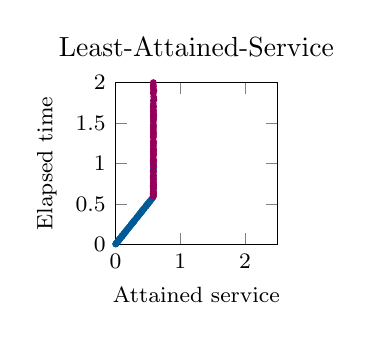
\begin{tikzpicture}

\begin{axis}[
    title=Least-Attained-Service,
    width=0.3\textwidth,
    height=0.3\textwidth,
    xlabel={Attained service},
    ylabel={Elapsed time},
    xmin=0,xmax=2.5,
    ymin=0,ymax=2,
    legend style={font=\footnotesize},
    legend cell align=left,
    legend pos=north east,
    ]
    \addplot[color=azulcito, only marks, mark={*}, mark size=1.0 pt, mark options={color=azulcito, draw opacity={1.0}, fill=azulcito}]
        table[row sep={\\}]
        {
            \\
            0.5874701902088146  1.0389792935178206  \\
            0.5874994123322278  0.9930669742239289  \\
            0.5877106095102251  0.9559513058323432  \\
            0.5874754561858566  0.940543836570058  \\
            0.5875298369836357  0.9265812355837544  \\
            0.5874701203821502  0.8530823170794775  \\
            0.5874910918763228  0.7342261225020721  \\
            0.5874923152883005  0.6537998921309622  \\
            0.5823237479178758  0.5823237479178758  \\
            0.5661973828557407  0.5661973828557407  \\
            0.5480575881387395  0.5480575881387395  \\
            0.5361795844943487  0.5361795844943487  \\
            0.5290161841918106  0.5290161841918106  \\
            0.5229846988227322  0.5229846988227322  \\
            0.5224289980559433  0.5224289980559438  \\
            0.5002625938194423  0.5002625938194427  \\
            0.499150685362018  0.499150685362018  \\
            0.4950520970011425  0.4950520970011425  \\
            0.4942312700501361  0.4942312700501361  \\
            0.4895271062404589  0.4895271062404589  \\
            0.48221054966228394  0.48221054966228394  \\
            0.4780601726852609  0.47806017268526135  \\
            0.4720133494616907  0.47201334946169027  \\
            0.4705060319212251  0.4705060319212251  \\
            0.46872438677772266  0.4687243867777231  \\
            0.4661589915703175  0.4661589915703175  \\
            0.4447245728159288  0.4447245728159288  \\
            0.4333548917224235  0.4333548917224235  \\
            0.4327650045175133  0.4327650045175133  \\
            0.43257890481435624  0.43257890481435624  \\
            0.42410000251761293  0.42410000251761204  \\
            0.4162624189055961  0.4162624189055961  \\
            0.4131217340975084  0.4131217340975084  \\
            0.4130159906163655  0.4130159906163655  \\
            0.39697017156215253  0.39697017156215253  \\
            0.3962943144291491  0.3962943144291491  \\
            0.38262474243785505  0.38262474243785505  \\
            0.38086350789552614  0.38086350789552625  \\
            0.3723577614756479  0.3723577614756479  \\
            0.3631199625941903  0.3631199625941903  \\
            0.35342176525975333  0.35342176525975333  \\
            0.3424114523520315  0.34241145235203163  \\
            0.3402487654183446  0.3402487654183446  \\
            0.3377450024680897  0.3377450024680897  \\
            0.32797497091460404  0.32797497091460315  \\
            0.312837319590045  0.3128373195900451  \\
            0.29816956130923744  0.29816956130923744  \\
            0.29246663828497077  0.29246663828497077  \\
            0.289790190185812  0.2897901901858124  \\
            0.2821527181425054  0.2821527181425054  \\
            0.2809270561238931  0.28092705612389324  \\
            0.2798525267399299  0.2798525267399299  \\
            0.27621133329824943  0.27621133329824943  \\
            0.2707798933132395  0.2707798933132399  \\
            0.2691026068215976  0.2691026068215976  \\
            0.2675394369424424  0.2675394369424424  \\
            0.2504428437705286  0.2504428437705286  \\
            0.2494197200166468  0.2494197200166468  \\
            0.23834622479683532  0.23834622479683532  \\
            0.23714389438598005  0.23714389438598005  \\
            0.2201174706063752  0.22011747060637532  \\
            0.22006293065552995  0.22006293065552995  \\
            0.21994508941163105  0.21994508941163105  \\
            0.21240738446427088  0.21240738446427088  \\
            0.19480416909040343  0.19480416909040343  \\
            0.1865568750220703  0.1865568750220703  \\
            0.18331423992659523  0.18331423992659523  \\
            0.18299439044450594  0.18299439044450594  \\
            0.16829380998951304  0.16829380998951393  \\
            0.16627194741343487  0.16627194741343487  \\
            0.16092674100473658  0.16092674100473658  \\
            0.14700568091756594  0.14700568091756594  \\
            0.14261303161890737  0.14261303161890737  \\
            0.13710697974114794  0.13710697974114794  \\
            0.13035061093914635  0.13035061093914635  \\
            0.1300754333605454  0.1300754333605454  \\
            0.1284195316335044  0.1284195316335044  \\
            0.11336065706355214  0.11336065706355214  \\
            0.11195458849308437  0.11195458849308437  \\
            0.10759279777010278  0.10759279777010278  \\
            0.10549720785022032  0.10549720785022032  \\
            0.1038685966252686  0.1038685966252686  \\
            0.10229564652397727  0.10229564652397727  \\
            0.09868588750069307  0.09868588750069307  \\
            0.09643707188418915  0.09643707188418915  \\
            0.09285744710128796  0.09285744710128796  \\
            0.07444916586199213  0.07444916586199213  \\
            0.07365673520099847  0.07365673520099847  \\
            0.06685474055366569  0.06685474055366569  \\
            0.061899584794808504  0.061899584794808504  \\
            0.05546600752696662  0.05546600752696662  \\
            0.05224637916035135  0.05224637916035135  \\
            0.04418581597481375  0.044185815974813636  \\
            0.03932184555819873  0.03932184555819873  \\
            0.039097593705761824  0.039097593705761824  \\
            0.021812346606758126  0.021812346606758126  \\
            0.01127862702380611  0.01127862702380611  \\
            0.010164417304494577  0.010164417304494577  \\
            0.00502007053882636  0.00502007053882636  \\
            0.004251440775824733  0.004251440775824733  \\
        }
        ;

    \addplot[color=rojito, only marks, mark={*}, mark size=1.0 pt, mark options={color=rojito, draw opacity={1.0}, fill=rojito}]
        table[row sep={\\}]
        {
            \\
            0.6424955598767852  35.85491305977929  \\
            0.6366814248469552  19.711500185878975  \\
            0.6372355731201722  16.66713671215416  \\
            0.639155177573544  15.526516205801705  \\
            0.641177727462904  14.274744141848306  \\
            0.6363431559803558  14.00489088419547  \\
            0.6380988161465364  11.951274737568147  \\
            0.6329404348096865  10.623143090430261  \\
            0.6310536183273037  9.970055037661474  \\
            0.631982849797545  9.689731481755445  \\
            0.6307122296411629  9.258496695787043  \\
            0.6328401982470879  8.710790115066873  \\
            0.6316586218078886  8.577632520493815  \\
            0.6332237497720428  8.454634177470572  \\
            0.6332100314356239  8.421640927847063  \\
            0.6303969080069951  8.316956239514198  \\
            0.6316630588075611  8.123499701755417  \\
            0.6332189568977613  8.015306403828284  \\
            0.6310707839393839  7.980786198381567  \\
            0.6309072384526146  7.460707505186441  \\
            0.6311102537808333  7.317122890923104  \\
            0.6341890977919267  6.8879575235375095  \\
            0.6322589064262338  6.773174396785253  \\
            0.6323156087252917  6.681625300386793  \\
            0.6310559938285056  6.298805380877798  \\
            0.6316499824189172  5.89462620678575  \\
            0.6304200323577911  5.651705467451471  \\
            0.5885282833483512  5.38827136319091  \\
            0.5915185573750286  4.974092088094496  \\
            0.5857657484908945  4.941033707605877  \\
            0.5865107174541118  4.8722188557311625  \\
            0.5899242219718195  4.868432723296842  \\
            0.5909296019924133  4.754490001816692  \\
            0.5858113337954407  4.715699202022886  \\
            0.5858214784792075  4.67625014396976  \\
            0.5862989081769348  4.548100912483957  \\
            0.5866600357069776  4.546992917670345  \\
            0.5909301953727049  4.457579128112375  \\
            0.5865147310929695  4.434943085180379  \\
            0.5909253342303362  4.403255072621411  \\
            0.5858682439924081  4.39345830543531  \\
            0.5865029652248261  4.381668237882209  \\
            0.5856461306670546  4.360547255554996  \\
            0.5861360866892884  4.3541386846251875  \\
            0.5863465824929497  4.231559119212781  \\
            0.5862967433433504  4.220551756219891  \\
            0.5858717650995215  4.152585428115932  \\
            0.5851480271643519  4.119718612081677  \\
            0.588059051977269  4.114650436218029  \\
            0.5857938189844698  4.094126195690181  \\
            0.5868112052108991  4.023793543349079  \\
            0.5865673429345579  3.9464571562426807  \\
            0.5868272335375044  3.9253784067949833  \\
            0.5852265698569408  3.9114981196190817  \\
            0.5859635964678205  3.8259699281394255  \\
            0.5851795807987941  3.7963908268391933  \\
            0.5915160706276934  3.776736314321688  \\
            0.5865670030246086  3.7508973863409643  \\
            0.5862739050915029  3.6729948933360257  \\
            0.5880684834673384  3.6521902969832145  \\
            0.5860160479787879  3.578515478093031  \\
            0.5852844686478562  3.4404722965716275  \\
            0.5910967816950352  3.3922935940294026  \\
            0.592064327080241  3.3847987424480133  \\
            0.5883984062881096  3.3303339498496594  \\
            0.5862931690943034  3.317380251294857  \\
            0.5859525248920407  3.296820963894246  \\
            0.5955048517280215  3.2863250995401363  \\
            0.5858290099624934  3.283011760835408  \\
            0.5884082312566283  3.212481324180955  \\
            0.5859812630931529  3.155354989332181  \\
            0.585603951842707  3.15258623186535  \\
            0.5880706831301916  3.1525278972900903  \\
            0.5955016712779615  3.1302891683037624  \\
            0.5862542223085638  3.123582370053015  \\
            0.5880917239111252  3.0778928723998185  \\
            0.5856438757614293  2.981305513662043  \\
            0.5859525290108056  2.91408070386627  \\
            0.5858620939636063  2.824841923660629  \\
            0.5871145152883601  2.760447615585511  \\
            0.5884056031376084  2.7555771171726917  \\
            0.5880193433049605  2.707897699559915  \\
            0.5852425709835685  2.672396711922247  \\
            0.5860123319874093  2.623552358500905  \\
            0.5852679286005573  2.6080647514265247  \\
            0.5868115888516128  2.5996608103325087  \\
            0.5855702636876003  2.599636082810335  \\
            0.5859335126960964  2.5813865033741825  \\
            0.5858955574880378  2.5511227041649684  \\
            0.5910993890788676  2.530750351431372  \\
            0.5868106051776869  2.506731923645838  \\
            0.592063033399783  2.433179814330999  \\
            0.5855645169880759  2.432128122561863  \\
            0.5861247180269782  2.3720218242528985  \\
            0.5858113173245311  2.357977482833796  \\
            0.5865044223668168  2.3542925994270703  \\
            0.5852839741138305  2.295735266925491  \\
            0.58523984128691  2.251442926669725  \\
            0.5856500852386968  2.229435542775086  \\
            0.5861399026939136  2.2073498446441926  \\
            0.5868291607249527  2.185080711032612  \\
            0.5898828972706331  2.1751246066582666  \\
            0.5900474723748541  2.1463259567064337  \\
            0.5865826499396523  2.113318334385914  \\
            0.5890526965299598  2.090836160229642  \\
            0.5856612511966608  2.032743882139023  \\
            0.5857814556987755  1.999419834069954  \\
            0.5855660297823428  1.9688751086721306  \\
            0.5857398459011343  1.9509836378872554  \\
            0.5857595972308887  1.9491078557632942  \\
            0.5859205687321181  1.9207028618408426  \\
            0.5954987942224652  1.8996847351864683  \\
            0.5863676577645681  1.8850031313784963  \\
            0.5851471030304674  1.8642535711631112  \\
            0.5910039925547368  1.8221549998557047  \\
            0.5955181051382348  1.7864175334713082  \\
            0.5854660528289424  1.7756870691719726  \\
            0.5856894427778938  1.7349050862553104  \\
            0.5857655101907131  1.7064686143827519  \\
            0.5857900089786492  1.7036498766486625  \\
            0.5861491533632746  1.6990897034251242  \\
            0.5859879061657658  1.6904817178060383  \\
            0.5859206853672383  1.6582062407160985  \\
            0.5857942883181915  1.654996216102243  \\
            0.5855974142060891  1.6521905579617169  \\
            0.5858651628963556  1.6367043906686334  \\
            0.5883169520586674  1.61704396195654  \\
            0.585880869998423  1.6097720277976926  \\
            0.5856835221551349  1.6095955960555934  \\
            0.5909385044103175  1.590178534031402  \\
            0.5858140680148328  1.5864385955168174  \\
            0.5904678835481318  1.5797055161094598  \\
            0.5851309314767095  1.575977838026398  \\
            0.5899479878985696  1.5471951319850716  \\
            0.585797723907201  1.5436989599014694  \\
            0.5856696399216326  1.5188870147368831  \\
            0.5863701902915901  1.4888824877580706  \\
            0.5865140403551173  1.4657302811222408  \\
            0.5859793323026032  1.4656359155840812  \\
            0.5855638667701459  1.4474665177678752  \\
            0.5860064636766285  1.4370011785862928  \\
            0.5857654080562795  1.4148884691658097  \\
            0.585633971693611  1.3998162491927038  \\
            0.5904322087671896  1.3724385842247244  \\
            0.5856005856351771  1.3704863612623654  \\
            0.586515901744551  1.3455732289390667  \\
            0.5851900015698992  1.330702312301426  \\
            0.5858048205290647  1.319520849799333  \\
            0.5859727140372755  1.276330802043462  \\
            0.5890806732059914  1.266936380436853  \\
            0.5851395908652823  1.263330705037498  \\
            0.5885827077668111  1.2445368636403642  \\
            0.5860664816605172  1.2227504868328651  \\
            0.586147490897809  1.2153372232666597  \\
            0.5861011339375679  1.1885033614359841  \\
            0.5884168036483142  1.169312573700445  \\
            0.5890671749334029  1.1655652465879527  \\
            0.5884330924763845  1.164937016135299  \\
            0.5851344634308369  1.1493069021840725  \\
            0.5859709471739811  1.1366582387959459  \\
            0.5855553715605192  1.1227575448807698  \\
            0.5884515746925267  1.1117914088873775  \\
            0.5887835297839858  1.1117541599950527  \\
            0.5856130210271866  1.0858756148466284  \\
            0.5856588447072015  1.0553274948023557  \\
            0.5834635302412359  1.0426712410526178  \\
            0.5836214951094627  1.0404841370838525  \\
            0.5855492992607052  1.0360436635183987  \\
            0.5856178828823551  1.0312259781443345  \\
            0.5854482155084298  1.0280116945162447  \\
            0.584210933894517  1.0171910981888246  \\
            0.5835774015406252  1.0036850667909576  \\
            0.5855759120310216  0.9834060231559718  \\
            0.5872880583358864  0.9662580419363778  \\
            0.5872246145376487  0.9596248353052488  \\
            0.5836948060353715  0.9094301663121982  \\
            0.5847108231578177  0.9047679711089258  \\
            0.5836039558876722  0.8991634830399207  \\
            0.5872072083192497  0.8875600838301452  \\
            0.5855378121856778  0.8532481786840052  \\
            0.5859280100142796  0.8491015028681312  \\
            0.5836364784553618  0.8381948045154601  \\
            0.583842815505918  0.8203437966096061  \\
            0.5856603914957415  0.8138448869091164  \\
            0.5859179494085385  0.8084365792683244  \\
            0.5854993682029748  0.8066955655356343  \\
            0.5847006031989379  0.8033480448512407  \\
            0.5874415713272398  0.7796629055878697  \\
            0.5854961689622852  0.7726792321143421  \\
            0.5836885211859757  0.7585963638844295  \\
            0.5880739379216757  0.74852920953861  \\
            0.583746674960413  0.7449754544424967  \\
            0.5837412435177534  0.7320969465030487  \\
            0.583724474520988  0.7260584890206374  \\
            0.5880747874292998  0.7244699796106744  \\
            0.5837476528939722  0.7179289554698731  \\
            0.5836278522625293  0.712759960022197  \\
            0.5874050242762001  0.702729514944231  \\
            0.5874206690326178  0.6980708775138069  \\
            0.5838398350254176  0.6944851202775908  \\
            0.5875111861055382  0.6855567472856734  \\
            0.5847109228388976  0.6838060687621947  \\
            0.5847630497338836  0.6559541558735522  \\
            0.5837365175225104  0.6475934017952127  \\
            0.5859280078781945  0.6325800454762316  \\
            0.585919592184446  0.6291897323688502  \\
            0.5857941673959262  0.6286542650998754  \\
            0.5837951140022999  0.6284701673185538  \\
            0.5841763910728801  0.6269659808705512  \\
            0.5842898661790985  0.6165241357329663  \\
            0.584390046390411  0.6062023929971687  \\
            0.5856293840402453  0.6023129466909563  \\
            0.5853169311301016  0.596595558153906  \\
            0.5837397349294866  0.5931355224709787  \\
        }
        ;
    \addplot[color=violetita,solid, very thick]
        table[row sep={\\}]
        {
            \\
            0.0  0.0  \\
            0.593  0.593  \\
            0.593  10.0  \\
        }
        ;
\end{axis}
\end{tikzpicture}

    \tikzsetnextfilename{lognormal_lcfs_statespace}
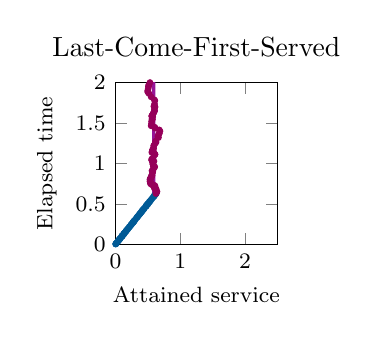
\begin{tikzpicture}
    \begin{axis}[
     title=Last-Come-First-Served,
    width=0.3\textwidth,
    height=0.3\textwidth,
    xlabel={Attained service},
    ylabel={Elapsed time},
    xmin=0,xmax=2.5,
    ymin=0,ymax=2,
    legend style={font=\footnotesize},
    legend cell align=left,
    legend pos=north east,
    ]

    \addplot[color=azulcito, only marks, mark={*}, mark size=1.0 pt, mark options={color=azulcito, draw opacity={1.0}, fill=azulcito}]
        table[row sep={\\}]
        {
            \\
            0.6286542650998614  0.6286542650998612  \\
            0.6284701673185396  0.6284701673185396  \\
            0.626965980870537  0.626965980870537  \\
            0.6165241357329523  0.6165241357329521  \\
            0.6062023929971545  0.6062023929971545  \\
            0.6023129466909434  0.6023129466909438  \\
            0.5965955581538931  0.5965955581538935  \\
            0.5931355224709653  0.5931355224709662  \\
            0.5823237479178616  0.5823237479178616  \\
            0.5661973828557265  0.5661973828557265  \\
            0.5480575881387253  0.5480575881387253  \\
            0.5361795844943344  0.5361795844943344  \\
            0.5290161841917964  0.5290161841917964  \\
            0.522984698822718  0.522984698822718  \\
            0.5224289980559291  0.5224289980559291  \\
            0.5002625938194294  0.5002625938194285  \\
            0.4991506853620038  0.4991506853620038  \\
            0.4950520970011283  0.4950520970011283  \\
            0.4942312700501219  0.4942312700501219  \\
            0.4895271062404447  0.4895271062404447  \\
            0.4822105496622697  0.4822105496622697  \\
            0.4780601726852467  0.4780601726852467  \\
            0.47201334946167606  0.47201334946167606  \\
            0.4705060319212109  0.4705060319212109  \\
            0.46872438677770845  0.46872438677770845  \\
            0.46615899157030327  0.46615899157030327  \\
            0.4447245728159146  0.4447245728159146  \\
            0.43335489172240926  0.43335489172240926  \\
            0.4327650045174991  0.4327650045174991  \\
            0.432578904814342  0.432578904814342  \\
            0.4241000025175983  0.42410000251759783  \\
            0.4162624189055819  0.4162624189055819  \\
            0.4131217340974942  0.4131217340974942  \\
            0.4130159906163513  0.4130159906163513  \\
            0.3969701715621383  0.3969701715621383  \\
            0.39629431442913443  0.39629431442913443  \\
            0.38262474243784084  0.38262474243784084  \\
            0.38086350789551193  0.38086350789551204  \\
            0.3723577614756337  0.3723577614756337  \\
            0.3631199625941761  0.3631199625941761  \\
            0.3534217652597391  0.3534217652597391  \\
            0.3424114523520173  0.3424114523520174  \\
            0.3402487654183304  0.3402487654183304  \\
            0.3377450024680755  0.3377450024680755  \\
            0.3279749709145894  0.32797497091458894  \\
            0.3128373195900308  0.3128373195900309  \\
            0.2981695613092228  0.2981695613092228  \\
            0.29246663828495656  0.29246663828495656  \\
            0.28979019018579777  0.28979019018579777  \\
            0.2821527181424912  0.2821527181424912  \\
            0.2809270561238789  0.280927056123879  \\
            0.2798525267399157  0.2798525267399157  \\
            0.2762113332982352  0.2762113332982352  \\
            0.2707798933132253  0.2707798933132253  \\
            0.2691026068215834  0.2691026068215834  \\
            0.2675394369424282  0.2675394369424282  \\
            0.2504428437705144  0.2504428437705144  \\
            0.2494197200166397  0.2494197200166397  \\
            0.2383462247968282  0.2383462247968282  \\
            0.23714389438597294  0.23714389438597294  \\
            0.2201174706063681  0.22011747060636822  \\
            0.22006293065552285  0.22006293065552285  \\
            0.21994508941162394  0.21994508941162394  \\
            0.21240738446426377  0.21240738446426377  \\
            0.19480416909039633  0.19480416909039633  \\
            0.1865568750220632  0.1865568750220632  \\
            0.18331423992658813  0.18331423992658813  \\
            0.18299439044449883  0.18299439044449883  \\
            0.16829380998950771  0.16829380998950683  \\
            0.16627194741342777  0.16627194741342777  \\
            0.16092674100472948  0.16092674100472948  \\
            0.14700568091755883  0.14700568091755883  \\
            0.14261303161890737  0.14261303161890737  \\
            0.13710697974114794  0.13710697974114794  \\
            0.13035061093914635  0.13035061093914635  \\
            0.1300754333605454  0.1300754333605454  \\
            0.1284195316335044  0.1284195316335044  \\
            0.11336065706355214  0.11336065706355214  \\
            0.11195458849308437  0.11195458849308437  \\
            0.10759279777010278  0.10759279777010278  \\
            0.10549720785022032  0.10549720785022032  \\
            0.1038685966252686  0.1038685966252686  \\
            0.10229564652397727  0.10229564652397727  \\
            0.09868588750069307  0.09868588750069307  \\
            0.09643707188418915  0.09643707188418915  \\
            0.09285744710128796  0.09285744710128796  \\
            0.07444916586199213  0.07444916586199213  \\
            0.07365673520099847  0.07365673520099847  \\
            0.06685474055366569  0.06685474055366569  \\
            0.061899584794808504  0.061899584794808504  \\
            0.05546600752696662  0.05546600752696662  \\
            0.05224637916035135  0.05224637916035135  \\
            0.04418581597481375  0.044185815974813636  \\
            0.03932184555819873  0.03932184555819873  \\
            0.039097593705761824  0.039097593705761824  \\
            0.021812346606758126  0.021812346606758126  \\
            0.01127862702380611  0.01127862702380611  \\
            0.010164417304494577  0.010164417304494577  \\
            0.00502007053882636  0.00502007053882636  \\
            0.004251440775824733  0.004251440775824733  \\
        }
        ;

    \addplot[color=rojito, only marks, mark={*}, mark size=1.0 pt, mark options={color=rojito, draw opacity={1.0}, fill=rojito}]
        table[row sep={\\}]
        {
            \\
            0.6336544299528342  35.85491305977946  \\
            0.5271209502335843  19.71150018587889  \\
            0.6045414716797382  16.667136712154065  \\
            0.6269725661556169  15.52651620580166  \\
            0.5732606832443903  14.27474414184825  \\
            0.5673469519236995  14.004890884195408  \\
            0.6915930151984622  11.951274737568072  \\
            0.5757575029419  10.6231430904302  \\
            0.5556770199991341  9.970055037661385  \\
            0.5357326103471394  9.689731481755356  \\
            0.6817731793915769  9.258496695786981  \\
            0.6024378135141966  8.710790115066814  \\
            0.5574150106128659  8.577632520493745  \\
            0.6064219859708295  8.454634177470503  \\
            0.617938060370796  8.421640927846997  \\
            0.6046043568105874  8.316956239514134  \\
            0.6456227760449949  8.123499701755321  \\
            0.6981835129051754  8.0153064038282  \\
            0.6933578535127651  7.980786198381496  \\
            0.5632166886181675  7.460707505186365  \\
            0.5078131010872466  7.317122890923028  \\
            0.5943921181081517  6.887957523537446  \\
            0.6172627533637041  6.773174396785185  \\
            0.6157822668507809  6.681625300386731  \\
            0.5731904908056862  6.298805380877738  \\
            0.869634020900806  5.894626206785701  \\
            0.6781703450967322  5.651705467451421  \\
            0.5628999479318448  5.388271363190835  \\
            0.5819371852451312  4.9740920880944675  \\
            0.5661143019070494  4.941033707605847  \\
            0.5187788310844823  4.872218855731134  \\
            0.5257522026853341  4.868432723296814  \\
            0.49541139627644526  4.754490001816663  \\
            0.4951474458030001  4.715699202022856  \\
            0.45996897118001456  4.67625014396973  \\
            0.4693394162975091  4.548100912483925  \\
            0.4682536463973226  4.546992917670317  \\
            0.5132031400665937  4.457579128112343  \\
            0.5117076959149225  4.4349430851803495  \\
            0.5442404460107744  4.4032550726213815  \\
            0.5353497701748111  4.393458305435281  \\
            0.5497875888932002  4.381668237882181  \\
            0.5735635049610011  4.3605472555549625  \\
            0.5751330011553328  4.3541386846251555  \\
            0.6083300378471979  4.2315591192127515  \\
            0.6196041014335112  4.2205517562198605  \\
            0.6704733170079038  4.152585428115904  \\
            0.6753905969883087  4.119718612081647  \\
            0.6759180559412377  4.114650436218  \\
            0.6676683736300291  4.0941261956901505  \\
            0.6389948009010666  4.023793543349049  \\
            0.6221628101127195  3.9464571562426514  \\
            0.6390533072548479  3.9253784067949535  \\
            0.6254697290637088  3.9114981196190524  \\
            0.6129955813058379  3.8259699281393935  \\
            0.6334518037630694  3.796390826839164  \\
            0.6295706400389971  3.776736314321658  \\
            0.6438001815650107  3.7508973863409354  \\
            0.6472167917001528  3.6729948933359964  \\
            0.6316919296649162  3.6521902969831848  \\
            0.5764527316344612  3.578515478093001  \\
            0.5564376984217176  3.4404722965713432  \\
            0.5589561735649564  3.392293594029373  \\
            0.5564100286419205  3.384798742447984  \\
            0.5226795591694247  3.3303339498496305  \\
            0.5569326357093427  3.3173802512948276  \\
            0.5412438467215539  3.296820963894217  \\
            0.5376720539537265  3.2863250995401074  \\
            0.5743658458582956  3.2830117608353797  \\
            0.5835957539257475  3.212481324180926  \\
            0.5556941789996657  3.155354989332152  \\
            0.5529501490550075  3.1525862318653215  \\
            0.5549200865935395  3.152527897290062  \\
            0.5415728653644871  3.130289168303733  \\
            0.535544907777088  3.123582370052987  \\
            0.5267701682348491  3.07789287239979  \\
            0.5481256993310444  2.981305513662014  \\
            0.543083409970265  2.91408070386624  \\
            0.5291066567351388  2.8248419236605997  \\
            0.5235172245209734  2.760447615585483  \\
            0.5261415743976058  2.7555771171726633  \\
            0.5232488962114878  2.707897699559876  \\
            0.5293433415054762  2.6723967119222256  \\
            0.6131281711084968  2.6235523585008806  \\
            0.6218735633686026  2.608064751426503  \\
            0.6316143340414007  2.5996608103324865  \\
            0.6373282146134684  2.599636082810317  \\
            0.6386537843021711  2.581386503374161  \\
            0.622213939723423  2.551122704164939  \\
            0.6264284910181883  2.5307503514313434  \\
            0.6294099690272406  2.5067319236458085  \\
            0.6611233251906015  2.4331798143309697  \\
            0.6746938031908092  2.4321281225618345  \\
            0.7170256081506539  2.372021824252867  \\
            0.7057869248720792  2.3579774828337667  \\
            0.7102075122540494  2.3542925994270396  \\
            0.6756007800682933  2.295735266925462  \\
            0.6418473306141332  2.2514429266696965  \\
            0.6346262624764569  2.2294355427750565  \\
            0.6279807291694914  2.2073498446441633  \\
            0.609102873006214  2.1850807110325805  \\
            0.6314256467567954  2.175124606658235  \\
            0.6305344024701798  2.146325956706403  \\
            0.6020733401941403  2.1133183343858857  \\
            0.5896011444676426  2.090836160229613  \\
            0.551694969458189  2.032743882138994  \\
            0.5336895529477097  1.9994198340699256  \\
            0.5139490508115552  1.9688751086721012  \\
            0.5098370699497803  1.9509836378872256  \\
            0.5121066771770022  1.9491078557632657  \\
            0.5058143926750267  1.9207028618408142  \\
            0.4998684859937579  1.8996847351864399  \\
            0.49821470693815684  1.8850031313784679  \\
            0.5171019111144273  1.8642535711630828  \\
            0.5517475286450262  1.8221549998556763  \\
            0.6000850805423776  1.7864175334712797  \\
            0.6093709489232109  1.7756870691719442  \\
            0.6043297669772789  1.7349050862552815  \\
            0.5947378224075313  1.7064686143827226  \\
            0.5966172253793549  1.7036498766486332  \\
            0.6124208230785957  1.699089703425095  \\
            0.6063169074203221  1.6904817178060094  \\
            0.5998556010846365  1.6582062407160691  \\
            0.6035996644890456  1.6549962161022131  \\
            0.6057770755758942  1.6521905579616885  \\
            0.5977250971507999  1.636704390668605  \\
            0.5856044550643984  1.6170439619565116  \\
            0.5785460496533492  1.6097720277976642  \\
            0.5801491707488324  1.6095955960555637  \\
            0.5626901838683764  1.5901785340313737  \\
            0.5632294565497344  1.586438595516789  \\
            0.5625144179206245  1.5797055161094313  \\
            0.5760188635306842  1.5759778380263691  \\
            0.5637891088290843  1.5471951319850428  \\
            0.5714453008936091  1.543698959901441  \\
            0.5584305228394537  1.5188870147368547  \\
            0.5555404982729986  1.4888824877580422  \\
            0.5516414676386961  1.4657302811222124  \\
            0.560821995721156  1.4656359155840528  \\
            0.6082082832170173  1.4474665177678467  \\
            0.6108642722377057  1.4370011785862644  \\
            0.6761986730256027  1.4148884691657884  \\
            0.6879907263370417  1.3998162491926838  \\
            0.6773916252187322  1.372438584224703  \\
            0.6760012409847667  1.3704863612623441  \\
            0.6595970556730039  1.3455732289390454  \\
            0.6571918042492455  1.3307023123014048  \\
            0.6650669962623974  1.3195208497993116  \\
            0.6225309099124985  1.2763308020434474  \\
            0.6209901478493691  1.2669363804368388  \\
            0.6282748433133567  1.2633307050374762  \\
            0.6119568181641242  1.2445368636403424  \\
            0.5935607544640078  1.2227504868328438  \\
            0.5916972723628087  1.215337223266638  \\
            0.5900126307849902  1.1885033614359628  \\
            0.5727170155465302  1.1693125737004237  \\
            0.5806149799577849  1.1655652465879314  \\
            0.58404309092289  1.1649370161352772  \\
            0.5684928088160781  1.1493069021840512  \\
            0.5627128717201373  1.136658238795924  \\
            0.5997728460580305  1.1227575448807485  \\
            0.611528815067935  1.1117914088873633  \\
            0.6116982274348155  1.111754159995038  \\
            0.5908235178454868  1.0858756148466142  \\
            0.5610962247522195  1.0553274948023414  \\
            0.5608984111118067  1.0426712410526031  \\
            0.5644249960840861  1.0404841370838378  \\
            0.5649843353833788  1.038979293517806  \\
            0.5655376315971739  1.0360436635183845  \\
            0.5751919550763176  1.0312259781443203  \\
            0.5952466899987315  1.0280116945162305  \\
            0.5846121933744675  1.0171910981888104  \\
            0.5795850642733456  1.0036850667909434  \\
            0.5768045553183329  0.9930669742239147  \\
            0.5831577111266613  0.9834060231559576  \\
            0.5853945340408524  0.9662580419363636  \\
            0.6062030700454955  0.9596248353052346  \\
            0.6051245541460661  0.955951305832329  \\
            0.5925041050712139  0.9405438365700434  \\
            0.5810200085609418  0.9265812355837402  \\
            0.5647604975045448  0.909430166312184  \\
            0.5780201384965493  0.9047679711089112  \\
            0.5739046163942669  0.8991634830399065  \\
            0.5748675662765139  0.887560083830131  \\
            0.5607815403990346  0.8532481786839909  \\
            0.560653519106098  0.8530823170794628  \\
            0.5655213002082735  0.849101502868117  \\
            0.5583422777755302  0.8381948045154459  \\
            0.5441324633113567  0.8203437966095919  \\
            0.5429268762567858  0.8138448869091022  \\
            0.5376566859550846  0.8084365792683101  \\
            0.5367499364941253  0.8066955655356196  \\
            0.5342454380296429  0.8033480448512265  \\
            0.5326680707117395  0.7796629055878554  \\
            0.5446709644406625  0.7726792321143279  \\
            0.5386512744727909  0.7585963638844149  \\
            0.5430444865273922  0.7485292095385958  \\
            0.5628895217829277  0.744975454442482  \\
            0.5679041145299661  0.7342261225020579  \\
            0.5944939664034088  0.7320969465030487  \\
            0.5959830556600778  0.7260584890206232  \\
            0.6106177903303434  0.7244699796106602  \\
            0.6059743669767741  0.7179289554698585  \\
            0.6059838670473643  0.7127599600221828  \\
            0.6003426302504016  0.7027295149442168  \\
            0.5993849900130996  0.6980708775137927  \\
            0.6125190493387938  0.6944851202775766  \\
            0.6236571624908507  0.6855567472856592  \\
            0.6287847232506136  0.6838060687621805  \\
            0.6299203739523949  0.6559541558735376  \\
            0.6420147276683164  0.653799892130948  \\
            0.637428984490704  0.6475934017951985  \\
            0.6275599749373915  0.6325800454762174  \\
            0.6249382915930114  0.629189732368836  \\
        }
        ;
    \addplot[color=violetita,solid, very thick]
        table[row sep={\\}]
        {
            \\
            0.0  0.0  \\
            0.593  0.593  \\
            0.593  10.0  \\
        }
        ;
\end{axis}
\end{tikzpicture}

    \end{center}

	\vfill
	Blue dots are in service, red dots are not in service. 
\end{frame}

\begin{frame}{Stochastic threshold evolution}
	\begin{center}
	\tikzsetnextfilename{lognormal_edf_threshold}
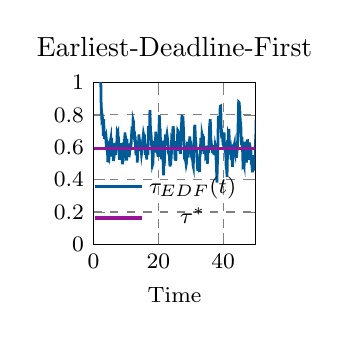
\begin{tikzpicture}
    \begin{axis}[
    title=Earliest-Deadline-First,
    width=0.3\textwidth,
    height=0.3\textwidth,
    xlabel={Time},
    ymin=0,ymax=1,
    xmin=0,xmax=50,
    grid,
    legend pos=south east,
    ]
    \addplot[color=azulcito, solid, line width=1pt]
        table[row sep={\\}]
        {
            \\
            0.8  3.804335929421449  \\
            0.9  2.908435875162442  \\
            1.0  2.045505050801774  \\
            1.1  1.7330744753242628  \\
            1.2  1.462759157889592  \\
            1.3  1.5330744753242629  \\
            1.4  1.3933521030224911  \\
            1.5  1.293352103022491  \\
            1.6  1.3848006161428277  \\
            1.7  1.2488101860995389  \\
            1.8  1.377247781511046  \\
            1.9  1.3373194294490944  \\
            2.0  1.213758552222619  \\
            2.1  1.169310973048041  \\
            2.2  1.0681400475285527  \\
            2.3  0.8882277940349532  \\
            2.4  0.8407960060104129  \\
            2.5  0.7958929242181016  \\
            2.6  0.8044038204658732  \\
            2.7  0.7916288778111151  \\
            2.8  0.7376203141599252  \\
            2.9  0.7567452614239314  \\
            3.0  0.6698320283401422  \\
            3.1  0.7733095104908272  \\
            3.2  0.7203495668708086  \\
            3.3  0.6664804852871395  \\
            3.4  0.6535119624082122  \\
            3.5  0.6969403571960573  \\
            3.6  0.6732483897510653  \\
            3.7  0.6739715630544993  \\
            3.8  0.6454035314292537  \\
            3.9  0.6561172173981688  \\
            4.0  0.6341367524166636  \\
            4.1  0.6386378212179606  \\
            4.2  0.6330985854057685  \\
            4.3  0.5745509853625905  \\
            4.4  0.5148661897282367  \\
            4.5  0.5144895379556234  \\
            4.6  0.5174114371849052  \\
            4.7  0.5530240207222434  \\
            4.8  0.5447032415679425  \\
            4.9  0.5708627613482805  \\
            5.0  0.5499096015548431  \\
            5.1  0.6198704815060587  \\
            5.2  0.6389135413023475  \\
            5.3  0.6505310527529429  \\
            5.4  0.5874270735158927  \\
            5.5  0.5422893017926524  \\
            5.6  0.6575371510598451  \\
            5.7  0.582718765791645  \\
            5.8  0.5598328300435758  \\
            5.9  0.5894918166041281  \\
            6.0  0.5639319313237134  \\
            6.1  0.5157511600175777  \\
            6.2  0.5307596395784455  \\
            6.3  0.5362713316951271  \\
            6.4  0.5590753880611863  \\
            6.5  0.5815499013454029  \\
            6.6  0.6261532467060034  \\
            6.7  0.5798693467158853  \\
            6.8  0.5543185388147789  \\
            6.9  0.5715355108643134  \\
            7.0  0.6050100693599179  \\
            7.1  0.618590201751994  \\
            7.2  0.6393299985685637  \\
            7.3  0.6927052717933364  \\
            7.4  0.6873445006010224  \\
            7.5  0.6924569274644832  \\
            7.6  0.640989857586642  \\
            7.7  0.664824462394292  \\
            7.8  0.6174903581414384  \\
            7.9  0.5824800053299883  \\
            8.0  0.5217661614300191  \\
            8.1  0.5922774840349723  \\
            8.2  0.565923537380927  \\
            8.3  0.5635811592855724  \\
            8.4  0.5704365245884606  \\
            8.5  0.6242191593123803  \\
            8.6  0.609409513356484  \\
            8.7  0.5538091453125265  \\
            8.8  0.5772024484280189  \\
            8.9  0.4952452693557312  \\
            9.0  0.5155453650994444  \\
            9.1  0.5444438433037515  \\
            9.2  0.541264199093801  \\
            9.3  0.6032887177578634  \\
            9.4  0.6000544165690602  \\
            9.5  0.6501899067041368  \\
            9.6  0.6341163279515101  \\
            9.7  0.6910636260669598  \\
            9.8  0.63799082536943  \\
            9.9  0.601828576871525  \\
            10.0  0.6116888784946877  \\
            10.1  0.5810244506558089  \\
            10.2  0.51789432024293  \\
            10.3  0.6530053642850602  \\
            10.4  0.5530053642850614  \\
            10.5  0.5854946261924692  \\
            10.6  0.5464567049255766  \\
            10.7  0.6156258342641543  \\
            10.8  0.5690965543887359  \\
            10.9  0.5479058829388989  \\
            11.0  0.5472777572653019  \\
            11.1  0.5602330374931463  \\
            11.2  0.624084961759845  \\
            11.3  0.6029943778703474  \\
            11.4  0.6133399811834401  \\
            11.5  0.5831092746220699  \\
            11.6  0.6227491969575958  \\
            11.7  0.6667808360643317  \\
            11.8  0.6970459931748949  \\
            11.9  0.7289556568759998  \\
            12.0  0.705462214154418  \\
            12.1  0.6868804837883733  \\
            12.2  0.7668521961428882  \\
            12.3  0.7586548198962819  \\
            12.4  0.7044237825857369  \\
            12.5  0.6902435397830522  \\
            12.6  0.6908341488536376  \\
            12.7  0.6342890941524661  \\
            12.8  0.6707004703428245  \\
            12.9  0.6445880890259925  \\
            13.0  0.5873444066073052  \\
            13.1  0.5510705732900321  \\
            13.2  0.5708609804459273  \\
            13.3  0.6144579694487802  \\
            13.4  0.6003603923450829  \\
            13.5  0.50478110534837  \\
            13.6  0.5769398663444938  \\
            13.7  0.6053145209537423  \\
            13.8  0.6259999926107636  \\
            13.9  0.6332870251161662  \\
            14.0  0.6785721251155512  \\
            14.1  0.6336567304642582  \\
            14.2  0.638838313014571  \\
            14.3  0.6230846506539685  \\
            14.4  0.5763705004673456  \\
            14.5  0.5910330949212508  \\
            14.6  0.6354365586815852  \\
            14.7  0.5840859699915625  \\
            14.8  0.5609962689313924  \\
            14.9  0.5762610761872171  \\
            15.0  0.6191762729284029  \\
            15.1  0.5980460069195993  \\
            15.2  0.6461054049845832  \\
            15.3  0.6629195963201086  \\
            15.4  0.6822311301781733  \\
            15.5  0.6719277015533007  \\
            15.6  0.6108309865844809  \\
            15.7  0.6799542954838339  \\
            15.8  0.6256098864326219  \\
            15.9  0.6237916151658508  \\
            16.0  0.5525390699210444  \\
            16.1  0.5850654426850034  \\
            16.2  0.5819992275515843  \\
            16.3  0.5793639433528989  \\
            16.4  0.5245810915395577  \\
            16.5  0.5861060191665786  \\
            16.6  0.6028228649651766  \\
            16.7  0.5710421680772733  \\
            16.8  0.5524019147653155  \\
            16.9  0.6980921234535984  \\
            17.0  0.7312865509879849  \\
            17.1  0.7083695798976134  \\
            17.2  0.692529684132019  \\
            17.3  0.7196976759747007  \\
            17.4  0.8295289342711105  \\
            17.5  0.749961229704621  \\
            17.6  0.6968981555133378  \\
            17.7  0.6920135092373094  \\
            17.8  0.6617108901631432  \\
            17.9  0.6227764663715121  \\
            18.0  0.5820467315315172  \\
            18.1  0.5592328787411027  \\
            18.2  0.4903826672678875  \\
            18.3  0.4967690518608762  \\
            18.4  0.5430223067717641  \\
            18.5  0.603141557390714  \\
            18.6  0.6386865941674178  \\
            18.7  0.6181372868831703  \\
            18.8  0.5892133683840801  \\
            18.9  0.5956112112703549  \\
            19.0  0.5793656176263262  \\
            19.1  0.6078682435491558  \\
            19.2  0.6964274242477813  \\
            19.3  0.6298299239903606  \\
            19.4  0.635349863179584  \\
            19.5  0.5636211452848303  \\
            19.6  0.6131016373865039  \\
            19.7  0.566352987566134  \\
            19.8  0.5629929568402925  \\
            19.9  0.5409484036878562  \\
            20.0  0.5707397848485058  \\
            20.1  0.6113371342151055  \\
            20.2  0.7042435438543997  \\
            20.3  0.7980296432539551  \\
            20.4  0.7438558050930233  \\
            20.5  0.6744090396836779  \\
            20.6  0.6786410079177756  \\
            20.7  0.6054635602409735  \\
            20.8  0.5701702580837313  \\
            20.9  0.5252093834149933  \\
            21.0  0.5799479432159158  \\
            21.1  0.5699706898932706  \\
            21.2  0.6408605021832194  \\
            21.3  0.6041292866884334  \\
            21.4  0.569450942536029  \\
            21.5  0.4904898762386869  \\
            21.6  0.42631867340250906  \\
            21.7  0.48522173548192526  \\
            21.8  0.48856082552469315  \\
            21.9  0.5122429461640801  \\
            22.0  0.6023018053954736  \\
            22.1  0.647632014777173  \\
            22.2  0.6783118944236186  \\
            22.3  0.621119566026934  \\
            22.4  0.6382369702913522  \\
            22.5  0.658691770657323  \\
            22.6  0.6709092261545418  \\
            22.7  0.6473036412026445  \\
            22.8  0.6170389132840004  \\
            22.9  0.6405113490465695  \\
            23.0  0.6242468088866602  \\
            23.1  0.5682653520939098  \\
            23.2  0.5624352232789782  \\
            23.3  0.5767826399511087  \\
            23.4  0.5434883739936502  \\
            23.5  0.5096108706966369  \\
            23.6  0.4806282068572969  \\
            23.7  0.5178678599272217  \\
            23.8  0.48835485211858654  \\
            23.9  0.5309968801084572  \\
            24.0  0.5357151457544717  \\
            24.1  0.6403981432894597  \\
            24.2  0.6339621617264903  \\
            24.3  0.6139996587793388  \\
            24.4  0.6376947069153331  \\
            24.5  0.7214606706206403  \\
            24.6  0.7219339147488846  \\
            24.7  0.7022744066338618  \\
            24.8  0.6146597297391772  \\
            24.9  0.5935071175775306  \\
            25.0  0.6135221617979667  \\
            25.1  0.5575223718350024  \\
            25.2  0.5223645075284846  \\
            25.3  0.5538616413548212  \\
            25.4  0.5168711628637155  \\
            25.5  0.5873069147307994  \\
            25.6  0.6112854606765588  \\
            25.7  0.6080035543130577  \\
            25.8  0.5785632161011165  \\
            25.9  0.6540047730542042  \\
            26.0  0.702741766957466  \\
            26.1  0.6988847478078846  \\
            26.2  0.6418911239764886  \\
            26.3  0.6458217018484689  \\
            26.4  0.641336795134805  \\
            26.5  0.6040660648353544  \\
            26.6  0.6400119525337957  \\
            26.7  0.5757749697714303  \\
            26.8  0.5586215603680031  \\
            26.9  0.630144668976687  \\
            27.0  0.6713596928637955  \\
            27.1  0.7356294396994407  \\
            27.2  0.7553946604136961  \\
            27.3  0.7998075084060936  \\
            27.4  0.7358928320727491  \\
            27.5  0.7173059144457071  \\
            27.6  0.7897083476477285  \\
            27.7  0.7364690793619602  \\
            27.8  0.6964000223430586  \\
            27.9  0.62805428239442  \\
            28.0  0.5675437523296019  \\
            28.1  0.5738241900268157  \\
            28.2  0.5475341719429676  \\
            28.3  0.5416918275063864  \\
            28.4  0.5165642239153705  \\
            28.5  0.5104735014321977  \\
            28.6  0.49411650011316155  \\
            28.7  0.5044834830603802  \\
            28.8  0.5701204140522518  \\
            28.9  0.6018979426514015  \\
            29.0  0.6347398408213962  \\
            29.1  0.5868801489739606  \\
            29.2  0.5360158523276404  \\
            29.3  0.6279499317493809  \\
            29.4  0.5823883344046048  \\
            29.5  0.5575463486280103  \\
            29.6  0.6231765266858247  \\
            29.7  0.6665781863160944  \\
            29.8  0.6370088403273932  \\
            29.9  0.635717471088519  \\
            30.0  0.623618082091685  \\
            30.1  0.60316352636886  \\
            30.2  0.5864447623919239  \\
            30.3  0.5313434265055896  \\
            30.4  0.571154318416923  \\
            30.5  0.5196189084929728  \\
            30.6  0.5382216265892303  \\
            30.7  0.49074956756878774  \\
            30.8  0.4816494806345122  \\
            30.9  0.610624051191003  \\
            31.0  0.6156454996634546  \\
            31.1  0.6682494837602313  \\
            31.2  0.7259617393320106  \\
            31.3  0.7383322783359496  \\
            31.4  0.6708250576402827  \\
            31.5  0.6440599264069533  \\
            31.6  0.6238231636109788  \\
            31.7  0.5691199034767178  \\
            31.8  0.591208626560803  \\
            31.9  0.5360330805029783  \\
            32.0  0.4982048181972729  \\
            32.1  0.469944766003759  \\
            32.2  0.45546089918524046  \\
            32.3  0.5031140075108889  \\
            32.4  0.5257870782127592  \\
            32.5  0.47289269945437695  \\
            32.6  0.49095363632682143  \\
            32.7  0.4459502136568927  \\
            32.8  0.5369420532839886  \\
            32.9  0.5567708478137698  \\
            33.0  0.5616659940243494  \\
            33.1  0.6569657727420335  \\
            33.2  0.6374993238318476  \\
            33.3  0.5754673649152977  \\
            33.4  0.5951139844055395  \\
            33.5  0.6756251113327563  \\
            33.6  0.6647607976176739  \\
            33.7  0.681838236192085  \\
            33.8  0.6446866177977788  \\
            33.9  0.6690799120593183  \\
            34.0  0.6178637851636736  \\
            34.1  0.5601401850602639  \\
            34.2  0.5892616407359696  \\
            34.3  0.5605836537002724  \\
            34.4  0.5878731455651274  \\
            34.5  0.6049008099272228  \\
            34.6  0.5563282791179491  \\
            34.7  0.5622894745240925  \\
            34.8  0.591886476260213  \\
            34.9  0.6076197872501011  \\
            35.0  0.5570793293282031  \\
            35.1  0.49860858710382816  \\
            35.2  0.512069737920227  \\
            35.3  0.6115947696368205  \\
            35.4  0.567997674737064  \\
            35.5  0.5698268356092483  \\
            35.6  0.6072301830853282  \\
            35.7  0.6535096018491315  \\
            35.8  0.7224416338774309  \\
            35.9  0.7433559431820065  \\
            36.0  0.772671687795552  \\
            36.1  0.7440144354973566  \\
            36.2  0.6548764700071388  \\
            36.3  0.6370086924670488  \\
            36.4  0.6173477841276814  \\
            36.5  0.6062228691969125  \\
            36.6  0.5877766808599025  \\
            36.7  0.5647107928521322  \\
            36.8  0.6138201446836683  \\
            36.9  0.5912544278960212  \\
            37.0  0.6130282316741855  \\
            37.1  0.5571626159841692  \\
            37.2  0.5762623802657805  \\
            37.3  0.5512688418036893  \\
            37.4  0.612136016724881  \\
            37.5  0.5695006255445003  \\
            37.6  0.607626621583834  \\
            37.7  0.5980417585502524  \\
            37.8  0.5407627970027065  \\
            37.9  0.49890745545344917  \\
            38.0  0.4449104950396079  \\
            38.1  0.38216117090219615  \\
            38.2  0.48535087801841037  \\
            38.3  0.51855721059462  \\
            38.4  0.631049211229004  \\
            38.5  0.7650590886313324  \\
            38.6  0.7934553845523453  \\
            38.7  0.7319080240422342  \\
            38.8  0.7340976861174937  \\
            38.9  0.7734619521465409  \\
            39.0  0.7885269139061251  \\
            39.1  0.852010466362664  \\
            39.2  0.8534301025921651  \\
            39.3  0.8183620463218658  \\
            39.4  0.718362046321864  \\
            39.5  0.6751458012942497  \\
            39.6  0.6541800164813978  \\
            39.7  0.683457019346564  \\
            39.8  0.6725152688905567  \\
            39.9  0.6412180781304428  \\
            40.0  0.6150094340853514  \\
            40.1  0.6443264217676715  \\
            40.2  0.5906652829472492  \\
            40.3  0.6924008546883655  \\
            40.4  0.6261252650547604  \\
            40.5  0.5909522164717562  \\
            40.6  0.585022009398223  \\
            40.7  0.5640898054659123  \\
            40.8  0.5961404391954801  \\
            40.9  0.4963484828209488  \\
            41.0  0.46255021246118855  \\
            41.1  0.4802498332851287  \\
            41.2  0.4162576003764642  \\
            41.3  0.5025610631387283  \\
            41.4  0.6432929664606064  \\
            41.5  0.6207209861894469  \\
            41.6  0.6728535565057092  \\
            41.7  0.6645395789500053  \\
            41.8  0.7126151409501416  \\
            41.9  0.6443219228037615  \\
            42.0  0.6000355063830012  \\
            42.1  0.6074009763223907  \\
            42.2  0.5896827081683962  \\
            42.3  0.596890685477717  \\
            42.4  0.5715486310537796  \\
            42.5  0.5211902685213654  \\
            42.6  0.6182603403602158  \\
            42.7  0.5594035385169747  \\
            42.8  0.5196844003204151  \\
            42.9  0.47888667848290156  \\
            43.0  0.551581849850515  \\
            43.1  0.6008626986003875  \\
            43.2  0.5767031269735757  \\
            43.3  0.5485301773026663  \\
            43.4  0.6112711000226196  \\
            43.5  0.6201623030070347  \\
            43.6  0.5734887859983195  \\
            43.7  0.5636770896085537  \\
            43.8  0.5998057140101807  \\
            43.9  0.5788459399394696  \\
            44.0  0.5354294339556294  \\
            44.1  0.5488855574225089  \\
            44.2  0.5813332069975774  \\
            44.3  0.5750037525272944  \\
            44.4  0.5928491686092556  \\
            44.5  0.6465669383155201  \\
            44.6  0.7138392196859797  \\
            44.7  0.7941150427691639  \\
            44.8  0.8796570590528487  \\
            44.9  0.8776121573759794  \\
            45.0  0.8727744897278948  \\
            45.1  0.8102193813581806  \\
            45.2  0.8245800149827005  \\
            45.3  0.7440853757402692  \\
            45.4  0.7578615157842705  \\
            45.5  0.7186099277755531  \\
            45.6  0.6387132184290827  \\
            45.7  0.6142442322285442  \\
            45.8  0.6622059789001181  \\
            45.9  0.6165207994489492  \\
            46.0  0.5946972085405164  \\
            46.1  0.5200312254376342  \\
            46.2  0.5281199237959273  \\
            46.3  0.4635867948895793  \\
            46.4  0.5093557474399119  \\
            46.5  0.49869753403715567  \\
            46.6  0.5992964120709843  \\
            46.7  0.5528360090409662  \\
            46.8  0.6351886913006127  \\
            46.9  0.5516090576273883  \\
            47.0  0.5453376185763122  \\
            47.1  0.5181636817794699  \\
            47.2  0.5055754314118135  \\
            47.3  0.6107716222896329  \\
            47.4  0.5966857148200047  \\
            47.5  0.6487129228021402  \\
            47.6  0.6281290910838351  \\
            47.7  0.5647373755944187  \\
            47.8  0.6213490717569714  \\
            47.9  0.5812724254762003  \\
            48.0  0.5225579669256399  \\
            48.1  0.6299154565075602  \\
            48.2  0.5926641250276612  \\
            48.3  0.6137756207925094  \\
            48.4  0.5601410389226228  \\
            48.5  0.557587648323896  \\
            48.6  0.5616218463941183  \\
            48.7  0.4933331513432224  \\
            48.8  0.5124912330857476  \\
            48.9  0.4931353685494523  \\
            49.0  0.46041341745530673  \\
            49.1  0.44506037243066743  \\
            49.2  0.5502736700479074  \\
            49.3  0.528190252949365  \\
            49.4  0.5355664129847071  \\
            49.5  0.5382091332974981  \\
            49.6  0.45621473214730246  \\
            49.7  0.5085756519389122  \\
            49.8  0.5331116953970678  \\
            49.9  0.5535038159808181  \\
            50.0  0.6367851841364427  \\
            50.1  0.6572152504127624  \\
            50.2  0.7692444765087512  \\
            50.3  0.7134250258506523  \\
            50.4  0.658962446575778  \\
            50.5  0.6589793688787964  \\
            50.6  0.6632323977750758  \\
            50.7  0.6382477772147581  \\
            50.8  0.6405471058581185  \\
            50.9  0.5968327703550083  \\
            51.0  0.6308888706698355  \\
            51.1  0.7157463747868462  \\
            51.2  0.7493908994520273  \\
            51.3  0.6616057719207546  \\
            51.4  0.6151763955300993  \\
            51.5  0.5709124930107938  \\
            51.6  0.5736018206020788  \\
            51.7  0.5437171038373654  \\
            51.8  0.545054942342702  \\
            51.9  0.5334250002691547  \\
            52.0  0.5203174439466878  \\
            52.1  0.5996563385363913  \\
            52.2  0.5480129910075959  \\
            52.3  0.5084192151096403  \\
            52.4  0.560451887125744  \\
            52.5  0.5948902432120349  \\
            52.6  0.6003050528178  \\
            52.7  0.5604043389371469  \\
            52.8  0.559197089989631  \\
            52.9  0.5013081978099265  \\
            53.0  0.4640755100566949  \\
            53.1  0.4613913907973881  \\
            53.2  0.559209189378522  \\
            53.3  0.572604822884756  \\
            53.4  0.58002992495922  \\
            53.5  0.624659388886414  \\
            53.6  0.62758409749982  \\
            53.7  0.5299477818307352  \\
            53.8  0.5410244544765921  \\
            53.9  0.5719185606355315  \\
            54.0  0.5789636545469254  \\
            54.1  0.5768997087312258  \\
            54.2  0.5953000297096236  \\
            54.3  0.6391443032620501  \\
            54.4  0.5540675611472352  \\
            54.5  0.6281723857567623  \\
            54.6  0.6169968439855822  \\
            54.7  0.6353351751669143  \\
            54.8  0.6210828510109678  \\
            54.9  0.599297396371206  \\
            55.0  0.6315641058693797  \\
            55.1  0.6329356018501571  \\
            55.2  0.5474150274272918  \\
            55.3  0.5474999305011039  \\
            55.4  0.5227879718138766  \\
            55.5  0.5128167427983144  \\
            55.6  0.557738208059575  \\
            55.7  0.5450040248142614  \\
            55.8  0.5127571716115824  \\
            55.9  0.5513434820064451  \\
            56.0  0.6196270828004962  \\
            56.1  0.6352146969102463  \\
            56.2  0.6091416440550859  \\
            56.3  0.603034644195233  \\
            56.4  0.6011596147222775  \\
            56.5  0.6407564914194377  \\
            56.6  0.684451654940744  \\
            56.7  0.6341291065595627  \\
            56.8  0.623907591769651  \\
            56.9  0.6347886397168665  \\
            57.0  0.6004775283568686  \\
            57.1  0.5351861182360262  \\
            57.2  0.5019716817517974  \\
            57.3  0.46117976253152904  \\
            57.4  0.5221656374196609  \\
            57.5  0.6088393457094414  \\
            57.6  0.5856730379855721  \\
            57.7  0.6207675412407916  \\
            57.8  0.6932916028541599  \\
            57.9  0.6500535924158009  \\
            58.0  0.6690815937313987  \\
            58.1  0.6372394055721955  \\
            58.2  0.6806415453750954  \\
            58.3  0.6629248702080699  \\
            58.4  0.6954858802524622  \\
            58.5  0.7632975533641966  \\
            58.6  0.7377202499021176  \\
            58.7  0.6722624992633941  \\
            58.8  0.6207697248986566  \\
            58.9  0.6972255528528488  \\
            59.0  0.6832843033284397  \\
            59.1  0.6660556459904541  \\
            59.2  0.6487068225194776  \\
            59.3  0.5992205542517138  \\
            59.4  0.6071416643449483  \\
            59.5  0.6341497693840734  \\
            59.6  0.627452131469687  \\
            59.7  0.5794272663750974  \\
            59.8  0.5681174156838875  \\
            59.9  0.6050678896002566  \\
            60.0  0.6292208581645653  \\
            60.1  0.6037581423887417  \\
            60.2  0.6141968626291145  \\
            60.3  0.6010893023362485  \\
            60.4  0.5893936328936888  \\
            60.5  0.5569897218831219  \\
            60.6  0.5694411386640894  \\
            60.7  0.5163520202754697  \\
            60.8  0.5496726619901793  \\
            60.9  0.5579400569084427  \\
            61.0  0.5872066823877731  \\
            61.1  0.5511628279311722  \\
            61.2  0.5926808380745294  \\
            61.3  0.58140214620515  \\
            61.4  0.5203093547004585  \\
            61.5  0.5397792599337947  \\
            61.6  0.5494677851616245  \\
            61.7  0.6099455783610708  \\
            61.8  0.5397882515617098  \\
            61.9  0.5365866096246776  \\
            62.0  0.5324758208566178  \\
            62.1  0.5678861555993218  \\
            62.2  0.5288670802171467  \\
            62.3  0.4970364560777787  \\
            62.4  0.513628849982446  \\
            62.5  0.4972158414663781  \\
            62.6  0.5161952425155074  \\
            62.7  0.48581250613159055  \\
            62.8  0.4908034201577891  \\
            62.9  0.5109261839461743  \\
            63.0  0.5561284234349342  \\
            63.1  0.5245431319237215  \\
            63.2  0.5538853029454955  \\
            63.3  0.5380352999225264  \\
            63.4  0.5305344809838104  \\
            63.5  0.6079301608736714  \\
            63.6  0.6798414407456981  \\
            63.7  0.6402995135188241  \\
            63.8  0.7047445410906545  \\
            63.9  0.6789461222280615  \\
            64.0  0.6485392120216338  \\
            64.1  0.6974712955804775  \\
            64.2  0.6802866513087666  \\
            64.3  0.6742968946582266  \\
            64.4  0.6221670958624657  \\
            64.5  0.6380193607744464  \\
            64.6  0.735065722377513  \\
            64.7  0.6798881362699234  \\
            64.8  0.6095733224613584  \\
            64.9  0.6304780455114951  \\
            65.0  0.6283717083724838  \\
            65.1  0.6502226134516462  \\
            65.2  0.5812973410896443  \\
            65.3  0.5952570759990402  \\
            65.4  0.5250234705951797  \\
            65.5  0.5756310826661099  \\
            65.6  0.5518491264280955  \\
            65.7  0.5548395053343855  \\
            65.8  0.58830942113471  \\
            65.9  0.5488194539517934  \\
            66.0  0.5589695277101049  \\
            66.1  0.5629701144259801  \\
            66.2  0.5430338924048925  \\
            66.3  0.5879772180298346  \\
            66.4  0.5408092887643017  \\
            66.5  0.6177732583666768  \\
            66.6  0.7040908631277318  \\
            66.7  0.6396351385041471  \\
            66.8  0.6847455798488791  \\
            66.9  0.6391564857203262  \\
            67.0  0.6077927857271137  \\
            67.1  0.5598890245049406  \\
            67.2  0.6075749862048648  \\
            67.3  0.6601976971882093  \\
            67.4  0.6185470339508863  \\
            67.5  0.6352757602515609  \\
            67.6  0.664519603545443  \\
            67.7  0.6371261346801287  \\
            67.8  0.547407367974472  \\
            67.9  0.5194907422331815  \\
            68.0  0.5614809649189043  \\
            68.1  0.5596432807900413  \\
            68.2  0.5624245420739535  \\
            68.3  0.5866409277001023  \\
            68.4  0.6024219745154511  \\
            68.5  0.5429786361773381  \\
            68.6  0.5257331421923945  \\
            68.7  0.5122050630513684  \\
            68.8  0.5193612957864671  \\
            68.9  0.520832533786391  \\
            69.0  0.5751330072318694  \\
            69.1  0.6031446137976246  \\
            69.2  0.5560048658303316  \\
            69.3  0.6661206072262473  \\
            69.4  0.7116786080127184  \\
            69.5  0.7002618254853985  \\
            69.6  0.7050861558362472  \\
            69.7  0.6656626542673367  \\
            69.8  0.6973971059295963  \\
            69.9  0.668959594106326  \\
            70.0  0.7072668376392102  \\
            70.1  0.6557136444117191  \\
            70.2  0.6857150848058851  \\
            70.3  0.7282507227874646  \\
            70.4  0.6628503060577629  \\
            70.5  0.7082909867883558  \\
            70.6  0.6486835498532031  \\
            70.7  0.5685075704311657  \\
            70.8  0.5439290753961101  \\
            70.9  0.6002213008338804  \\
            71.0  0.5510260751775543  \\
            71.1  0.5439645759414162  \\
            71.2  0.4772636225121545  \\
            71.3  0.5503845861444034  \\
            71.4  0.5424647519744941  \\
            71.5  0.581477370399842  \\
            71.6  0.6809824568819636  \\
            71.7  0.7275907746515538  \\
            71.8  0.6917243367892212  \\
            71.9  0.6519455357257584  \\
            72.0  0.6707632794368976  \\
            72.1  0.6795153958386364  \\
            72.2  0.6150821179132322  \\
            72.3  0.5781934207033572  \\
            72.4  0.5573684184946188  \\
            72.5  0.5444863613685271  \\
            72.6  0.5458637452704638  \\
            72.7  0.5931423336479469  \\
            72.8  0.5418696684776876  \\
            72.9  0.5586955756790104  \\
            73.0  0.511541183838915  \\
            73.1  0.4966845197259593  \\
            73.2  0.5838342413081703  \\
            73.3  0.5324230409751038  \\
            73.4  0.4963106318955113  \\
            73.5  0.5278039435011408  \\
            73.6  0.5254631167113999  \\
            73.7  0.5276246305556805  \\
            73.8  0.5227358202330663  \\
            73.9  0.5200754622689061  \\
            74.0  0.5294541402310387  \\
            74.1  0.69964278078871  \\
            74.2  0.6370856652278283  \\
            74.3  0.6223248943952626  \\
            74.4  0.676352660756592  \\
            74.5  0.6335131399413285  \\
            74.6  0.6290945741442471  \\
            74.7  0.6006047447271925  \\
            74.8  0.5475106591715049  \\
            74.9  0.6317287178195699  \\
            75.0  0.573465975966613  \\
            75.1  0.5291065056297557  \\
            75.2  0.519124864931328  \\
            75.3  0.5028680889362533  \\
            75.4  0.6318819582068189  \\
            75.5  0.6370906116043213  \\
            75.6  0.628639793825229  \\
            75.7  0.6478024739391812  \\
            75.8  0.7245659314076813  \\
            75.9  0.6714410344164885  \\
            76.0  0.6303435130259625  \\
            76.1  0.6391698662038863  \\
            76.2  0.6544092720214247  \\
            76.3  0.6274244344125604  \\
            76.4  0.6086979268872315  \\
            76.5  0.5805994010666712  \\
            76.6  0.6165312604590121  \\
            76.7  0.5933399387715216  \\
            76.8  0.5895970631161307  \\
            76.9  0.5980641191379306  \\
            77.0  0.5844742198965209  \\
            77.1  0.5879142730056801  \\
            77.2  0.6974537403778667  \\
            77.3  0.6583812616730563  \\
            77.4  0.631272807472985  \\
            77.5  0.6079837440597942  \\
            77.6  0.6480076548279783  \\
            77.7  0.6341497502516518  \\
            77.8  0.5964322551841126  \\
            77.9  0.6291592375257409  \\
            78.0  0.6227470510771672  \\
            78.1  0.6119026202476769  \\
            78.2  0.6218209621567632  \\
            78.3  0.6201306450025479  \\
            78.4  0.622279961784812  \\
            78.5  0.5958591394615951  \\
            78.6  0.574462779201681  \\
            78.7  0.6812705726871684  \\
            78.8  0.645050011932156  \\
            78.9  0.5750498490998412  \\
            79.0  0.6373568366642277  \\
            79.1  0.673688862096242  \\
            79.2  0.6716411086084548  \\
            79.3  0.7509501748380814  \\
            79.4  0.6613935103470701  \\
            79.5  0.7060257718446659  \\
            79.6  0.6856138787529886  \\
            79.7  0.7570836933786649  \\
            79.8  0.7236606866764244  \\
            79.9  0.6781894188707867  \\
            80.0  0.6288012987762102  \\
            80.1  0.6243889380240262  \\
            80.2  0.6039808269744342  \\
            80.3  0.5580752948540777  \\
            80.4  0.5586222318428051  \\
            80.5  0.5031005738492998  \\
            80.6  0.5307148706318556  \\
            80.7  0.4443117735440154  \\
            80.8  0.5207250916696422  \\
            80.9  0.5112414152307423  \\
            81.0  0.5466499896986119  \\
            81.1  0.4907331930668164  \\
            81.2  0.4846361738632643  \\
            81.3  0.4776724703765183  \\
            81.4  0.46713233389155473  \\
            81.5  0.44656943876556365  \\
            81.6  0.5208673197514218  \\
            81.7  0.5281197472392023  \\
            81.8  0.6204186378453755  \\
            81.9  0.6298781517889722  \\
            82.0  0.6601343475909118  \\
            82.1  0.6678900960793044  \\
            82.2  0.7509073634604508  \\
            82.3  0.6888514224319238  \\
            82.4  0.6808049813470092  \\
            82.5  0.6876625694826544  \\
            82.6  0.7997148806436911  \\
            82.7  0.7471345984468485  \\
            82.8  0.6670680545027494  \\
            82.9  0.6478627557623895  \\
            83.0  0.6586074642921158  \\
            83.1  0.6771949174381291  \\
            83.2  0.7202475316521566  \\
            83.3  0.6842713805127545  \\
            83.4  0.749452183405154  \\
            83.5  0.7157368448186645  \\
            83.6  0.7132420792517706  \\
            83.7  0.6500277737999571  \\
            83.8  0.6096320678017284  \\
            83.9  0.637635623830775  \\
            84.0  0.6125241805663961  \\
            84.1  0.5900641909689883  \\
            84.2  0.6167664081095694  \\
            84.3  0.675121370710599  \\
            84.4  0.6290278817710089  \\
            84.5  0.6175519137165679  \\
            84.6  0.5300738162823677  \\
            84.7  0.5503274037962171  \\
            84.8  0.5510410339201854  \\
            84.9  0.5362320877988935  \\
            85.0  0.5535793231918404  \\
            85.1  0.5641162766368808  \\
            85.2  0.5600664419671091  \\
            85.3  0.5281124820303376  \\
            85.4  0.6149175306930486  \\
            85.5  0.6122590313954959  \\
            85.6  0.6189766436851869  \\
            85.7  0.6379913523007019  \\
            85.8  0.7423812717126457  \\
            85.9  0.6773815289064231  \\
            86.0  0.6810937623454836  \\
            86.1  0.6323841377960028  \\
            86.2  0.5715153911453239  \\
            86.3  0.5432540910294961  \\
            86.4  0.593329960856595  \\
            86.5  0.6348551790896124  \\
            86.6  0.6704608542933101  \\
            86.7  0.643945852017282  \\
            86.8  0.7044844937809387  \\
            86.9  0.6965647791948584  \\
            87.0  0.6840494939236378  \\
            87.1  0.6206912118275199  \\
            87.2  0.5265646745795749  \\
            87.3  0.5708816582700961  \\
            87.4  0.5127107596963042  \\
            87.5  0.5298067496375438  \\
            87.6  0.526413145876798  \\
            87.7  0.5806923181009154  \\
            87.8  0.5442652134505863  \\
            87.9  0.532562531926871  \\
            88.0  0.545868298206102  \\
            88.1  0.5872248630195571  \\
            88.2  0.6236309751673876  \\
            88.3  0.5486456164695852  \\
            88.4  0.5977079685112869  \\
            88.5  0.5297910566364403  \\
            88.6  0.525426520926132  \\
            88.7  0.4983770072799416  \\
            88.8  0.5310487970665605  \\
            88.9  0.5355360664642745  \\
            89.0  0.5753350210091099  \\
            89.1  0.5998810602729217  \\
            89.2  0.552536889044049  \\
            89.3  0.4924299640438363  \\
            89.4  0.5095465634741467  \\
            89.5  0.5675069448032277  \\
            89.6  0.5332498959129881  \\
            89.7  0.571727331084346  \\
            89.8  0.6299626162968655  \\
            89.9  0.6545306072526529  \\
            90.0  0.6591245450401435  \\
            90.1  0.6579472324012426  \\
            90.2  0.7099222083337078  \\
            90.3  0.7153645233255193  \\
            90.4  0.6811119132620589  \\
            90.5  0.6376484930438555  \\
            90.6  0.572235187673499  \\
            90.7  0.551712650392922  \\
            90.8  0.5258733176230808  \\
            90.9  0.5060845916493975  \\
            91.0  0.516700538129399  \\
            91.1  0.5602075900817312  \\
            91.2  0.6705124490551668  \\
            91.3  0.6023832060091507  \\
            91.4  0.587747831722073  \\
            91.5  0.5537688561050518  \\
            91.6  0.5847186259536699  \\
            91.7  0.5967284546242264  \\
            91.8  0.5764785514250388  \\
            91.9  0.568886925957784  \\
            92.0  0.5364035008432353  \\
            92.1  0.4814990630709983  \\
            92.2  0.4637557944713533  \\
            92.3  0.45068610418250876  \\
            92.4  0.4752420607051271  \\
            92.5  0.45375500051867873  \\
            92.6  0.4331376895709411  \\
            92.7  0.5040482961325414  \\
            92.8  0.478886483356604  \\
            92.9  0.46884490772561127  \\
            93.0  0.5053049687226552  \\
            93.1  0.5156916373679932  \\
            93.2  0.5852279851661993  \\
            93.3  0.6188995822361463  \\
            93.4  0.5879400882931378  \\
            93.5  0.5590595536087188  \\
            93.6  0.5706563062242083  \\
            93.7  0.5462806445873696  \\
            93.8  0.49698121914347926  \\
            93.9  0.44903855981200014  \\
            94.0  0.5040762010803093  \\
            94.1  0.47041452529599237  \\
            94.2  0.582550807481909  \\
            94.3  0.6400651303629701  \\
            94.4  0.6620416698990255  \\
            94.5  0.6023333589762392  \\
            94.6  0.6415059305161465  \\
            94.7  0.5827562523288823  \\
            94.8  0.606587942211803  \\
            94.9  0.6426765396298999  \\
            95.0  0.6254303518575761  \\
            95.1  0.6299008256738432  \\
            95.2  0.6052123250156711  \\
            95.3  0.5959549063574796  \\
            95.4  0.6126326504909656  \\
            95.5  0.6149888864384963  \\
            95.6  0.5963330341035231  \\
            95.7  0.599242013048936  \\
            95.8  0.6084375689937502  \\
            95.9  0.6199588343188873  \\
            96.0  0.6646953452245432  \\
            96.1  0.6903568110406582  \\
            96.2  0.7193696041841662  \\
            96.3  0.7109952037863678  \\
            96.4  0.7074405515859633  \\
            96.5  0.6946446506329043  \\
            96.6  0.7536637507055981  \\
            96.7  0.7871808935667741  \\
            96.8  0.6929183797435456  \\
            96.9  0.6185051820183527  \\
            97.0  0.6258369343780197  \\
            97.1  0.6541312223129112  \\
            97.2  0.5636037930090372  \\
            97.3  0.5435184164744418  \\
            97.4  0.5691820271092922  \\
            97.5  0.560380063951996  \\
            97.6  0.6087332579389222  \\
            97.7  0.5834700589080057  \\
            97.8  0.6144361287194187  \\
            97.9  0.5633165395533837  \\
            98.0  0.6413309559226916  \\
            98.1  0.6326040052451702  \\
            98.2  0.6525980982017625  \\
            98.3  0.6991678001361805  \\
            98.4  0.6025558289275027  \\
            98.5  0.6129592423815484  \\
            98.6  0.6169209367379827  \\
            98.7  0.5613742205186727  \\
            98.8  0.5535567084620103  \\
            98.9  0.5817485874233912  \\
            99.0  0.5764037285781862  \\
            99.1  0.6139386134785099  \\
            99.2  0.5773222849383615  \\
            99.3  0.5684003402884636  \\
            99.4  0.5569163783715968  \\
            99.5  0.6275360737446936  \\
            99.6  0.6004234962776853  \\
            99.7  0.6002220067922652  \\
            99.8  0.6307861500124257  \\
            99.9  0.6670009751379241  \\
            100.0  0.6639378326022038  \\
        }
        ;
    \addlegendentry {$\tau_{EDF}(t)$}
    \addplot[color=violetita, solid, very thick]
        table[row sep={\\}]
        {
            \\
            0  0.593  \\
            100.0  0.593  \\
        }
        ;
    \addlegendentry {$\tau^*$}
\end{axis}
\end{tikzpicture}

    \tikzsetnextfilename{lognormal_las_threshold}
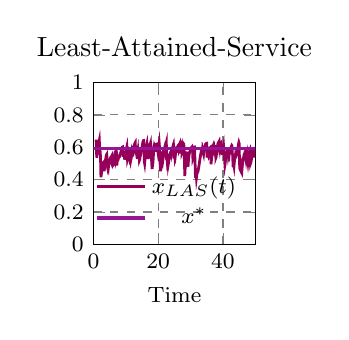
\begin{tikzpicture}
\begin{axis}[
    title=Least-Attained-Service,
    width=0.3\textwidth,
    height=0.3\textwidth,
    xlabel={Time},
    ymin=0,ymax=1,
    xmin=0,xmax=50,
    grid,
    legend pos=south east
    ]

    \addplot[color=rojito, solid, line width=1pt]
        table[row sep={\\}]        {
            \\
            0.8  0.6476176857286231  \\
            0.9  0.6144144751882679  \\
            1.0  0.5355318864489774  \\
            1.1  0.552378385195402  \\
            1.2  0.5647122438946013  \\
            1.3  0.5833383644641081  \\
            1.4  0.597250116878258  \\
            1.5  0.6116203174615877  \\
            1.6  0.6265643610848235  \\
            1.7  0.6331946205492811  \\
            1.8  0.6426148457396255  \\
            1.9  0.5990495861153291  \\
            2.0  0.5676785503829047  \\
            2.1  0.56830150378065  \\
            2.2  0.5177164958163991  \\
            2.3  0.4149499279719171  \\
            2.4  0.428311341480895  \\
            2.5  0.4450879127899463  \\
            2.6  0.4622240272175451  \\
            2.7  0.47275623917697407  \\
            2.8  0.48529507601210975  \\
            2.9  0.4978458954260706  \\
            3.0  0.5030929833545241  \\
            3.1  0.507010494796134  \\
            3.2  0.5090825229063248  \\
            3.3  0.45171955449704004  \\
            3.4  0.46799107454675815  \\
            3.5  0.48392835282826296  \\
            3.6  0.5031230915768663  \\
            3.7  0.519593726975486  \\
            3.8  0.5298330533905071  \\
            3.9  0.5434225157841854  \\
            4.0  0.5528556175970483  \\
            4.1  0.5562936578570887  \\
            4.2  0.5349173515662752  \\
            4.3  0.4820768398586348  \\
            4.4  0.47146285833770274  \\
            4.5  0.4808839740214088  \\
            4.6  0.4727587467080365  \\
            4.7  0.49084098623643424  \\
            4.8  0.49918867971384673  \\
            4.9  0.506845090247821  \\
            5.0  0.5143571476908101  \\
            5.1  0.5196140308613786  \\
            5.2  0.5292903610923334  \\
            5.3  0.5371956422643795  \\
            5.4  0.5398958867685737  \\
            5.5  0.5409854264826226  \\
            5.6  0.5448270270135792  \\
            5.7  0.497584938432432  \\
            5.8  0.49240346483817876  \\
            5.9  0.4859756868832772  \\
            6.0  0.4892134297493902  \\
            6.1  0.4914023953030551  \\
            6.2  0.5109551482960294  \\
            6.3  0.5203098922373091  \\
            6.4  0.5375527543676462  \\
            6.5  0.5522708882709662  \\
            6.6  0.5623154180709058  \\
            6.7  0.5686891481199217  \\
            6.8  0.5731686112255039  \\
            6.9  0.5741874945919712  \\
            7.0  0.5184303325269086  \\
            7.1  0.5251582654754947  \\
            7.2  0.48689900451894985  \\
            7.3  0.5081111123614397  \\
            7.4  0.5355865767503912  \\
            7.5  0.5243121048403099  \\
            7.6  0.5236930043305135  \\
            7.7  0.5304488576925612  \\
            7.8  0.5365567536977988  \\
            7.9  0.5392519210657074  \\
            8.0  0.5401212260744135  \\
            8.1  0.5441921012691715  \\
            8.2  0.5488677957448829  \\
            8.3  0.5597576968766781  \\
            8.4  0.5661681593302843  \\
            8.5  0.5735136892146652  \\
            8.6  0.583043618225709  \\
            8.7  0.5898750015447507  \\
            8.8  0.5960990775101855  \\
            8.9  0.6009372429737905  \\
            9.0  0.6019864647206035  \\
            9.1  0.5700807321640904  \\
            9.2  0.5412381272060192  \\
            9.3  0.5625873135806301  \\
            9.4  0.5701454727413593  \\
            9.5  0.568478324102589  \\
            9.6  0.523639373017887  \\
            9.7  0.5364978665349778  \\
            9.8  0.5498882122373212  \\
            9.9  0.5628807694110485  \\
            10.0  0.574374867224833  \\
            10.1  0.5783636719333056  \\
            10.2  0.5930018928696263  \\
            10.3  0.6018888087766293  \\
            10.4  0.5623800383001072  \\
            10.5  0.5287120577673861  \\
            10.6  0.537058369093266  \\
            10.7  0.5654321708169647  \\
            10.8  0.5741227166784572  \\
            10.9  0.5669212735044793  \\
            11.0  0.5540009173302605  \\
            11.1  0.5741733497086998  \\
            11.2  0.5737254637633811  \\
            11.3  0.5835946069731186  \\
            11.4  0.5827266754022782  \\
            11.5  0.5579870260361781  \\
            11.6  0.5284820020338712  \\
            11.7  0.5384210693176392  \\
            11.8  0.5474684006391408  \\
            11.9  0.5694219148650497  \\
            12.0  0.5606363664614908  \\
            12.1  0.5430133122278225  \\
            12.2  0.5747121942232277  \\
            12.3  0.5897552607238943  \\
            12.4  0.6000404579734513  \\
            12.5  0.6079000167646003  \\
            12.6  0.6133036063213689  \\
            12.7  0.6186651893805712  \\
            12.8  0.6253797078610637  \\
            12.9  0.6289422559611525  \\
            13.0  0.563156389242149  \\
            13.1  0.5852628671131788  \\
            13.2  0.5508792606825244  \\
            13.3  0.5799282593769304  \\
            13.4  0.5712540086982552  \\
            13.5  0.5266202493615779  \\
            13.6  0.5625592989963755  \\
            13.7  0.5754779152387535  \\
            13.8  0.5443421371544486  \\
            13.9  0.5779615454794831  \\
            14.0  0.5608372375985589  \\
            14.1  0.5640440003072767  \\
            14.2  0.5204626709382119  \\
            14.3  0.5257030415515924  \\
            14.4  0.5407836272072952  \\
            14.5  0.5473793809948242  \\
            14.6  0.5657617312578496  \\
            14.7  0.5798641910545452  \\
            14.8  0.5861906224307463  \\
            14.9  0.5943510286534335  \\
            15.0  0.6028844619731377  \\
            15.1  0.6132444391071061  \\
            15.2  0.6251431916901642  \\
            15.3  0.6362803641353416  \\
            15.4  0.6407687183622066  \\
            15.5  0.6412743912325565  \\
            15.6  0.5858724341581176  \\
            15.7  0.5116639924625335  \\
            15.8  0.5004531607947342  \\
            15.9  0.5228124661377489  \\
            16.0  0.5461383266921789  \\
            16.1  0.5689032321296024  \\
            16.2  0.5864364518191728  \\
            16.3  0.5987812227526286  \\
            16.4  0.6121646522843562  \\
            16.5  0.6211506526600452  \\
            16.6  0.5932819921634047  \\
            16.7  0.622041243772538  \\
            16.8  0.5269339231664958  \\
            16.9  0.5632626838305829  \\
            17.0  0.5453112975101178  \\
            17.1  0.568281861764986  \\
            17.2  0.584454119021474  \\
            17.3  0.5774753974648696  \\
            17.4  0.5974534394093443  \\
            17.5  0.6182156223568009  \\
            17.6  0.6246804435711899  \\
            17.7  0.5751064793289768  \\
            17.8  0.5808878108077398  \\
            17.9  0.5399017598404718  \\
            18.0  0.49981073557755096  \\
            18.1  0.46570986064929887  \\
            18.2  0.48062046951033377  \\
            18.3  0.4945363650909763  \\
            18.4  0.5134708661646498  \\
            18.5  0.5487742324655436  \\
            18.6  0.5780618795813819  \\
            18.7  0.5962974826186221  \\
            18.8  0.609590334627512  \\
            18.9  0.6040861923805574  \\
            19.0  0.5722851488633225  \\
            19.1  0.6006902794610482  \\
            19.2  0.6166115581973344  \\
            19.3  0.6185684443079811  \\
            19.4  0.6191998029249435  \\
            19.5  0.5898426190199506  \\
            19.6  0.6202281660943312  \\
            19.7  0.5975463089872157  \\
            19.8  0.5841858307227297  \\
            19.9  0.6080137407842328  \\
            20.0  0.6211041869071225  \\
            20.1  0.6219860045778729  \\
            20.2  0.6097472800376837  \\
            20.3  0.624454412348602  \\
            20.4  0.5992859220455817  \\
            20.5  0.5193042081760955  \\
            20.6  0.4913306414595091  \\
            20.7  0.4513908793820285  \\
            20.8  0.4692312971167571  \\
            20.9  0.48139272446436343  \\
            21.0  0.5072175344723031  \\
            21.1  0.5246314818687967  \\
            21.2  0.5440804367975787  \\
            21.3  0.5612427471178512  \\
            21.4  0.569023019579312  \\
            21.5  0.5740280114543925  \\
            21.6  0.5428477418729507  \\
            21.7  0.5565014297354409  \\
            21.8  0.5721047359252951  \\
            21.9  0.5809079909605916  \\
            22.0  0.5949035493881976  \\
            22.1  0.6075469120332242  \\
            22.2  0.6151131551558886  \\
            22.3  0.6231561059110093  \\
            22.4  0.6211904454560511  \\
            22.5  0.6290519397088696  \\
            22.6  0.5194981036921398  \\
            22.7  0.5326239160187284  \\
            22.8  0.507699703347054  \\
            22.9  0.5164304881942816  \\
            23.0  0.532792592188027  \\
            23.1  0.49419600376238493  \\
            23.2  0.5052479580985827  \\
            23.3  0.5303125484760982  \\
            23.4  0.5444088798442976  \\
            23.5  0.5554375023849383  \\
            23.6  0.5570610798636286  \\
            23.7  0.5625671528794063  \\
            23.8  0.5609484368844164  \\
            23.9  0.5668199200944322  \\
            24.0  0.5563734935834006  \\
            24.1  0.5693368914102641  \\
            24.2  0.5757486860860062  \\
            24.3  0.5819249789354739  \\
            24.4  0.5917323938677979  \\
            24.5  0.6021350691849943  \\
            24.6  0.611077476288796  \\
            24.7  0.6170526381452779  \\
            24.8  0.5860903063395215  \\
            24.9  0.5303479971688212  \\
            25.0  0.5718758510542306  \\
            25.1  0.5488848177425936  \\
            25.2  0.5629733752637232  \\
            25.3  0.5524996417095869  \\
            25.4  0.5710651014623498  \\
            25.5  0.5779103378085164  \\
            25.6  0.5715482476994977  \\
            25.7  0.5729201056727433  \\
            25.8  0.5845413298487232  \\
            25.9  0.5938767620243341  \\
            26.0  0.6020829081901672  \\
            26.1  0.6085167544925074  \\
            26.2  0.6125145218416534  \\
            26.3  0.6146978257547733  \\
            26.4  0.5935730685150948  \\
            26.5  0.6020277420310298  \\
            26.6  0.6179456495211648  \\
            26.7  0.6229906713007534  \\
            26.8  0.5998962845970333  \\
            26.9  0.5609992234618844  \\
            27.0  0.6024954960519855  \\
            27.1  0.6057944510157309  \\
            27.2  0.6117279532867528  \\
            27.3  0.5643465061574771  \\
            27.4  0.5694414211587533  \\
            27.5  0.5821639512007228  \\
            27.6  0.6038074782608613  \\
            27.7  0.6158073676335336  \\
            27.8  0.6222439257375987  \\
            27.9  0.6193841908254636  \\
            28.0  0.5755882202729871  \\
            28.1  0.513707898494399  \\
            28.2  0.42240453387469756  \\
            28.3  0.4627698464770127  \\
            28.4  0.48457861954392056  \\
            28.5  0.4846722563145164  \\
            28.6  0.4996194621186558  \\
            28.7  0.51889515340687  \\
            28.8  0.5411227563888845  \\
            28.9  0.5562486081187168  \\
            29.0  0.572919468474625  \\
            29.1  0.5434380820402751  \\
            29.2  0.4787054776524293  \\
            29.3  0.5101464415755756  \\
            29.4  0.5332455236274553  \\
            29.5  0.5494587741375254  \\
            29.6  0.5598457715172729  \\
            29.7  0.5687231018782599  \\
            29.8  0.5740694694316062  \\
            29.9  0.5809038135127398  \\
            30.0  0.5867118425809554  \\
            30.1  0.5898388243267654  \\
            30.2  0.59530647303737  \\
            30.3  0.5991315190664501  \\
            30.4  0.6016343484370332  \\
            30.5  0.586003374311801  \\
            30.6  0.5877126074696579  \\
            30.7  0.5307975367800921  \\
            30.8  0.5367107087382021  \\
            30.9  0.5604103425032312  \\
            31.0  0.5849278416685009  \\
            31.1  0.6012583585426379  \\
            31.2  0.6016109366235827  \\
            31.3  0.5443884116194366  \\
            31.4  0.4868384887429472  \\
            31.5  0.4115141231719113  \\
            31.6  0.4329100008093185  \\
            31.7  0.4372227351065101  \\
            31.8  0.4118012937437251  \\
            31.9  0.42660082771733676  \\
            32.0  0.44065505174469033  \\
            32.1  0.444280656385718  \\
            32.2  0.4451931074638851  \\
            32.3  0.45334103042817997  \\
            32.4  0.4654907579608978  \\
            32.5  0.4766706639723415  \\
            32.6  0.48709467338067536  \\
            32.7  0.5020444485547544  \\
            32.8  0.5164859167754878  \\
            32.9  0.5299778576487139  \\
            33.0  0.5421089999899271  \\
            33.1  0.5551688073688263  \\
            33.2  0.5653779619758056  \\
            33.3  0.5767211533960586  \\
            33.4  0.5806290437967112  \\
            33.5  0.5872787002518955  \\
            33.6  0.5668230614243885  \\
            33.7  0.5904717755969373  \\
            33.8  0.5835460220559057  \\
            33.9  0.5649986040451732  \\
            34.0  0.5573270105058858  \\
            34.1  0.5759864843873852  \\
            34.2  0.5967582785317513  \\
            34.3  0.6026450305616025  \\
            34.4  0.6050819872453079  \\
            34.5  0.61141395623892  \\
            34.6  0.6181798687461755  \\
            34.7  0.6219777295457138  \\
            34.8  0.6229268118278863  \\
            34.9  0.6244280485484115  \\
            35.0  0.6248527705984235  \\
            35.1  0.535993578003271  \\
            35.2  0.5520862267725017  \\
            35.3  0.5603816547741691  \\
            35.4  0.55396060574546  \\
            35.5  0.5683909344711999  \\
            35.6  0.5717624747222825  \\
            35.7  0.575672190074348  \\
            35.8  0.5842592636398369  \\
            35.9  0.5933498314791077  \\
            36.0  0.5961373638490888  \\
            36.1  0.5982479695476927  \\
            36.2  0.5668194686460803  \\
            36.3  0.49479523029670247  \\
            36.4  0.5138929262921081  \\
            36.5  0.5393403949476081  \\
            36.6  0.5674001121930887  \\
            36.7  0.5826027994732286  \\
            36.8  0.5969141721366613  \\
            36.9  0.6052428050219589  \\
            37.0  0.6104385995408865  \\
            37.1  0.5898410920759933  \\
            37.2  0.5806950642022817  \\
            37.3  0.589043217456759  \\
            37.4  0.5736343891420799  \\
            37.5  0.5709262714307004  \\
            37.6  0.5989242374361211  \\
            37.7  0.6129367032955804  \\
            37.8  0.534880517134214  \\
            37.9  0.5402615949441403  \\
            38.0  0.5809293952288739  \\
            38.1  0.5521230002104293  \\
            38.2  0.5771850352546863  \\
            38.3  0.6030732519236891  \\
            38.4  0.6189599992492009  \\
            38.5  0.6253485535412233  \\
            38.6  0.6294975322702476  \\
            38.7  0.6316123823616557  \\
            38.8  0.6356434829535873  \\
            38.9  0.6062768928691322  \\
            39.0  0.5919910461786984  \\
            39.1  0.608485872010007  \\
            39.2  0.6233348149791462  \\
            39.3  0.625575524482997  \\
            39.4  0.5898774109903612  \\
            39.5  0.586280172700711  \\
            39.6  0.6211684985347143  \\
            39.7  0.5845402528077244  \\
            39.8  0.5530173830663185  \\
            39.9  0.5702750172141147  \\
            40.0  0.5748773051317748  \\
            40.1  0.5878210069696022  \\
            40.2  0.6008889738021419  \\
            40.3  0.5713088242878257  \\
            40.4  0.569678579045565  \\
            40.5  0.5237858636790667  \\
            40.6  0.49201554857547125  \\
            40.7  0.503483768287031  \\
            40.8  0.525727236808911  \\
            40.9  0.537665586551455  \\
            41.0  0.5459206477890897  \\
            41.1  0.5552435039591928  \\
            41.2  0.5638999951939843  \\
            41.3  0.5753639457784255  \\
            41.4  0.584735435959185  \\
            41.5  0.5881018293641449  \\
            41.6  0.5881310903111805  \\
            41.7  0.549630290742428  \\
            41.8  0.5589036855128549  \\
            41.9  0.5515853601145164  \\
            42.0  0.569334983043848  \\
            42.1  0.5764265018870672  \\
            42.2  0.5811585899607739  \\
            42.3  0.5883925282108217  \\
            42.4  0.5917968676304295  \\
            42.5  0.5962685645227195  \\
            42.6  0.6067932440736157  \\
            42.7  0.6111300006776317  \\
            42.8  0.6078629504742852  \\
            42.9  0.5578253686912915  \\
            43.0  0.5506172645992986  \\
            43.1  0.4846476082976592  \\
            43.2  0.4828469775357709  \\
            43.3  0.496178305253125  \\
            43.4  0.4841412610250009  \\
            43.5  0.5072436133730223  \\
            43.6  0.5227488630042314  \\
            43.7  0.534267029258082  \\
            43.8  0.5478700618251422  \\
            43.9  0.5375093539196385  \\
            44.0  0.5393381148579124  \\
            44.1  0.5523811493603441  \\
            44.2  0.5540448914688563  \\
            44.3  0.558624816014117  \\
            44.4  0.569429027796962  \\
            44.5  0.5809989923658153  \\
            44.6  0.5946262067857448  \\
            44.7  0.6082626663191104  \\
            44.8  0.6199497957617026  \\
            44.9  0.6288166638976191  \\
            45.0  0.6221340650833156  \\
            45.1  0.5016276851649764  \\
            45.2  0.4678358197771857  \\
            45.3  0.4633441243494547  \\
            45.4  0.4912609221448352  \\
            45.5  0.5168750615484539  \\
            45.6  0.47091451121620054  \\
            45.7  0.4630607749559912  \\
            45.8  0.48076681078720096  \\
            45.9  0.46980252835041547  \\
            46.0  0.4923709834962331  \\
            46.1  0.5047997816414689  \\
            46.2  0.5204852734662859  \\
            46.3  0.5290758199829474  \\
            46.4  0.5425369137828064  \\
            46.5  0.5520987679532809  \\
            46.6  0.5587781161596992  \\
            46.7  0.5632061132630319  \\
            46.8  0.5708281724305531  \\
            46.9  0.5740831230408028  \\
            47.0  0.5404722965715933  \\
            47.1  0.5266951160929443  \\
            47.2  0.5432273376516575  \\
            47.3  0.5521206940477963  \\
            47.4  0.4907822857983958  \\
            47.5  0.5290801664188027  \\
            47.6  0.5225087988683298  \\
            47.7  0.5078976995599156  \\
            47.8  0.5259682506205011  \\
            47.9  0.5448357295690565  \\
            48.0  0.5583426024821729  \\
            48.1  0.5660341752926114  \\
            48.2  0.5767936976798742  \\
            48.3  0.5821758800319371  \\
            48.4  0.5625392641005007  \\
            48.5  0.4996847351864697  \\
            48.6  0.5052905612386455  \\
            48.7  0.5295660503346031  \\
            48.8  0.5520581563044711  \\
            48.9  0.5626117415682228  \\
            49.0  0.5543823905744175  \\
            49.1  0.5680272646583971  \\
            49.2  0.5825365571391594  \\
            49.3  0.5843637387700213  \\
            49.4  0.5851216325359991  \\
            49.5  0.5702147673451425  \\
            49.6  0.5652153059997076  \\
            49.7  0.5365445959867748  \\
            49.8  0.5690900475432581  \\
            49.9  0.5836948060353715  \\
            50.0  0.5876463222646828  \\
            50.1  0.592063033399783  \\
            50.2  0.5983153735475908  \\
            50.3  0.6029173701848758  \\
            50.4  0.6056750661738732  \\
            50.5  0.6096416313238868  \\
            50.6  0.6135377288677075  \\
            50.7  0.6141737117957116  \\
            50.8  0.6156024314028237  \\
            50.9  0.5531389713444312  \\
            51.0  0.5844301682805761  \\
            51.1  0.5936245206989459  \\
            51.2  0.613194105085964  \\
            51.3  0.5447219057432302  \\
            51.4  0.558045467837627  \\
            51.5  0.5355886285375078  \\
            51.6  0.49942703965183455  \\
            51.7  0.4448062029627824  \\
            51.8  0.4606876288126287  \\
            51.9  0.4537693820018738  \\
            52.0  0.45605477998473276  \\
            52.1  0.4716313779193162  \\
            52.2  0.4873196229937622  \\
            52.3  0.5022827346857286  \\
            52.4  0.510899002331408  \\
            52.5  0.5241700095336612  \\
            52.6  0.5374599790674591  \\
            52.7  0.5508060185994386  \\
            52.8  0.557241583044574  \\
            52.9  0.5604157326915531  \\
            53.0  0.5345127237620134  \\
            53.1  0.5468170858449355  \\
            53.2  0.4942472130925637  \\
            53.3  0.5175569726205229  \\
            53.4  0.5412850757112144  \\
            53.5  0.5468288014889628  \\
            53.6  0.528930686935142  \\
            53.7  0.5318448450765274  \\
            53.8  0.5355979187637212  \\
            53.9  0.5400974655851074  \\
            54.0  0.5295091286830882  \\
            54.1  0.5443331828987574  \\
            54.2  0.5514822003502862  \\
            54.3  0.5030327671255608  \\
            54.4  0.4486265208213498  \\
            54.5  0.4749633125454982  \\
            54.6  0.5057579265245808  \\
            54.7  0.5292728515576807  \\
            54.8  0.5366498237053907  \\
            54.9  0.5478103071315026  \\
            55.0  0.5538036166998803  \\
            55.1  0.5248143562961611  \\
            55.2  0.5398483364271199  \\
            55.3  0.5573447211438254  \\
            55.4  0.5587614859559613  \\
            55.5  0.5607350512837779  \\
            55.6  0.5634291759906553  \\
            55.7  0.4811377863251991  \\
            55.8  0.46213740025635963  \\
            55.9  0.4708643896373482  \\
            56.0  0.48986116464691776  \\
            56.1  0.5020863987253346  \\
            56.2  0.5185079287821992  \\
            56.3  0.533273646398331  \\
            56.4  0.5507898954369154  \\
            56.5  0.5663844132109523  \\
            56.6  0.572902858204098  \\
            56.7  0.578904553870859  \\
            56.8  0.5811940348705829  \\
            56.9  0.5756791832295587  \\
            57.0  0.5623131687058205  \\
            57.1  0.5290663943783613  \\
            57.2  0.5277039757965579  \\
            57.3  0.560333991305824  \\
            57.4  0.57840148190779  \\
            57.5  0.5839928232756417  \\
            57.6  0.5910325173700679  \\
            57.7  0.5983448746844786  \\
            57.8  0.6071227669340082  \\
            57.9  0.6105547543415124  \\
            58.0  0.6145524980101946  \\
            58.1  0.6159528572391486  \\
            58.2  0.5398567487570025  \\
            58.3  0.5579967084617756  \\
            58.4  0.4921254626471243  \\
            58.5  0.5236680520490394  \\
            58.6  0.5461431591575308  \\
            58.7  0.5589400227897199  \\
            58.8  0.5073280277602299  \\
            58.9  0.5601962824804545  \\
            59.0  0.5706254241675301  \\
            59.1  0.5791850647901207  \\
            59.2  0.5855415871095462  \\
            59.3  0.5881526515411579  \\
            59.4  0.59613381864618  \\
            59.5  0.5980478491271539  \\
            59.6  0.5134778732044945  \\
            59.7  0.49543228373304427  \\
            59.8  0.4715578186189987  \\
            59.9  0.47811141982449934  \\
            60.0  0.4956203413314938  \\
            60.1  0.512503413259173  \\
            60.2  0.5331363658198529  \\
            60.3  0.5549508714488867  \\
            60.4  0.5685407342359636  \\
            60.5  0.5733463245667565  \\
            60.6  0.5747859141488134  \\
            60.7  0.5422185562733688  \\
            60.8  0.4590037521754744  \\
            60.9  0.4605730719636939  \\
            61.0  0.47375422510517323  \\
            61.1  0.4974108553850418  \\
            61.2  0.5045411582681611  \\
            61.3  0.5221614760140953  \\
            61.4  0.5331553673310516  \\
            61.5  0.5462406319110426  \\
            61.6  0.5597015510079204  \\
            61.7  0.5667743395191589  \\
            61.8  0.5629984307546465  \\
            61.9  0.5422578950991925  \\
            62.0  0.536767179881165  \\
            62.1  0.4813449530413103  \\
            62.2  0.5071150779362625  \\
            62.3  0.52140940652677  \\
            62.4  0.5458616850961863  \\
            62.5  0.5613042263963064  \\
            62.6  0.5648662872766068  \\
            62.7  0.5736423352935587  \\
            62.8  0.5792911340853233  \\
            62.9  0.5810108137648999  \\
            63.0  0.5139656665964774  \\
            63.1  0.5558923030150078  \\
            63.2  0.5803185261257031  \\
            63.3  0.5854039632680221  \\
            63.4  0.5882427911683727  \\
            63.5  0.5970414341265613  \\
            63.6  0.6054641166355463  \\
            63.7  0.6143020439265219  \\
            63.8  0.6185360371237034  \\
            63.9  0.6202896311695767  \\
            64.0  0.5536205359049475  \\
            64.1  0.5614843699406507  \\
            64.2  0.5793954331091056  \\
            64.3  0.5884157258434046  \\
            64.4  0.5507982885418068  \\
            64.5  0.5703172309815703  \\
            64.6  0.5947159549995121  \\
            64.7  0.6068517260330224  \\
            64.8  0.6019631862491384  \\
            64.9  0.5631523933214027  \\
            65.0  0.5646644374071033  \\
            65.1  0.48915482222753326  \\
            65.2  0.42916644964083206  \\
            65.3  0.4459319776989211  \\
            65.4  0.45659050650758193  \\
            65.5  0.47038022816317415  \\
            65.6  0.48525650699797773  \\
            65.7  0.5131366656521015  \\
            65.8  0.5387458896292662  \\
            65.9  0.5516075111017869  \\
            66.0  0.5612775273345876  \\
            66.1  0.5743921880658505  \\
            66.2  0.5360479029416042  \\
            66.3  0.5178014859863533  \\
            66.4  0.5452134271998255  \\
            66.5  0.5525884187888421  \\
            66.6  0.5692341413974145  \\
            66.7  0.5770217029521798  \\
            66.8  0.5826963353716987  \\
            66.9  0.5875150725558465  \\
            67.0  0.5913763580745992  \\
            67.1  0.5954131749793321  \\
            67.2  0.6003718588077089  \\
            67.3  0.5611936357627486  \\
            67.4  0.5336719268540615  \\
            67.5  0.5689019017165818  \\
            67.6  0.5658800542414751  \\
            67.7  0.5778698992740772  \\
            67.8  0.577426808083928  \\
            67.9  0.5862535083932714  \\
            68.0  0.5962650727597099  \\
            68.1  0.571984329911672  \\
            68.2  0.55121427988108  \\
            68.3  0.5712307061379817  \\
            68.4  0.5891498154684698  \\
            68.5  0.5535180058578826  \\
            68.6  0.5821577660042712  \\
            68.7  0.5968628552337647  \\
            68.8  0.6027674346658185  \\
            68.9  0.5587303166949056  \\
            69.0  0.596769516592488  \\
            69.1  0.6063598051151251  \\
            69.2  0.5431056509294196  \\
            69.3  0.5475342327373767  \\
            69.4  0.5610728222306702  \\
            69.5  0.6005866456102082  \\
            69.6  0.6102938540003349  \\
            69.7  0.6055781379604799  \\
            69.8  0.6138239809835675  \\
            69.9  0.6181590513888446  \\
            70.0  0.6236609813108029  \\
            70.1  0.6279151954834576  \\
            70.2  0.6284162485251805  \\
            70.3  0.6262504707832611  \\
            70.4  0.6295622293251022  \\
            70.5  0.6299058994624991  \\
            70.6  0.606401378191749  \\
            70.7  0.5822976699667919  \\
            70.8  0.5768399659554431  \\
            70.9  0.5915187892328606  \\
            71.0  0.5544263302635388  \\
            71.1  0.513451754258524  \\
            71.2  0.4980987588479453  \\
            71.3  0.5035717536826927  \\
            71.4  0.4976439578525307  \\
            71.5  0.5132132795806257  \\
            71.6  0.5283480968222329  \\
            71.7  0.5429220444438294  \\
            71.8  0.5582366822359718  \\
            71.9  0.5672799299058651  \\
            72.0  0.5823457768120321  \\
            72.1  0.5939421117336678  \\
            72.2  0.604805453772955  \\
            72.3  0.6123705583947534  \\
            72.4  0.5981698060516436  \\
            72.5  0.6081590785025948  \\
            72.6  0.5800158694557913  \\
            72.7  0.5451509027930828  \\
            72.8  0.5174033927249004  \\
            72.9  0.5168667338114543  \\
            73.0  0.4787911009370306  \\
            73.1  0.45728946091006106  \\
            73.2  0.48851943546434395  \\
            73.3  0.5160394116740532  \\
            73.4  0.5295279477247457  \\
            73.5  0.5411432412474739  \\
            73.6  0.5533193950659334  \\
            73.7  0.5565620889116498  \\
            73.8  0.5477584410665344  \\
            73.9  0.5347778256121964  \\
            74.0  0.5597435106602973  \\
            74.1  0.5686852115324665  \\
            74.2  0.5733245036641903  \\
            74.3  0.5828042543617036  \\
            74.4  0.5857264824499855  \\
            74.5  0.5896693324423357  \\
            74.6  0.5496568418872271  \\
            74.7  0.5620956762881925  \\
            74.8  0.563565798164829  \\
            74.9  0.5771729465316007  \\
            75.0  0.5286185116453767  \\
            75.1  0.513599252552666  \\
            75.2  0.526554445829845  \\
            75.3  0.548119246463938  \\
            75.4  0.577774900932154  \\
            75.5  0.5925836635756951  \\
            75.6  0.6015975679356624  \\
            75.7  0.6155033926227736  \\
            75.8  0.6244058976272526  \\
            75.9  0.6296554686897032  \\
            76.0  0.6228042947555396  \\
            76.1  0.6224787470323179  \\
            76.2  0.5303165054609031  \\
            76.3  0.551571964801894  \\
            76.4  0.5545052679278369  \\
            76.5  0.5775320227327545  \\
            76.6  0.592551587749749  \\
            76.7  0.6117979573758447  \\
            76.8  0.6281581628303341  \\
            76.9  0.5449173704326  \\
            77.0  0.5842199574707667  \\
            77.1  0.6016062939116784  \\
            77.2  0.6189952789887104  \\
            77.3  0.5807301590387919  \\
            77.4  0.5498904236498696  \\
            77.5  0.5672373310815395  \\
            77.6  0.5462098073375898  \\
            77.7  0.5082382695157166  \\
            77.8  0.5408494294179165  \\
            77.9  0.5642441783272325  \\
            78.0  0.5712943483791513  \\
            78.1  0.5831824779432964  \\
            78.2  0.6003801336588901  \\
            78.3  0.6205911343033244  \\
            78.4  0.6287957557196124  \\
            78.5  0.6334443927671185  \\
            78.6  0.6353858474533514  \\
            78.7  0.6359007305176194  \\
            78.8  0.5872940250239085  \\
            78.9  0.5578024886306987  \\
            79.0  0.5813884235271725  \\
            79.1  0.601441292248134  \\
            79.2  0.6115155094071301  \\
            79.3  0.6204027458059755  \\
            79.4  0.5723741598668254  \\
            79.5  0.5657087413940618  \\
            79.6  0.544566470312944  \\
            79.7  0.5421303251888361  \\
            79.8  0.5513031127013761  \\
            79.9  0.5647312424034816  \\
            80.0  0.5663933039440561  \\
            80.1  0.5731682652725709  \\
            80.2  0.5787483310341739  \\
            80.3  0.5400027687769295  \\
            80.4  0.5671370164430892  \\
            80.5  0.4992362358973139  \\
            80.6  0.5336090458916534  \\
            80.7  0.508440495027543  \\
            80.8  0.5274708056295624  \\
            80.9  0.5013378497792038  \\
            81.0  0.5193169077745796  \\
            81.1  0.5273374856165427  \\
            81.2  0.537082000785843  \\
            81.3  0.5091833104633561  \\
            81.4  0.5432386266988841  \\
            81.5  0.5532277299802707  \\
            81.6  0.5619866760507082  \\
            81.7  0.5673273311843723  \\
            81.8  0.5828900368414162  \\
            81.9  0.5974344039982284  \\
            82.0  0.6121271885614561  \\
            82.1  0.6178095185610637  \\
            82.2  0.6228716190667303  \\
            82.3  0.626619378951343  \\
            82.4  0.6328022183180528  \\
            82.5  0.6361430134237009  \\
            82.6  0.6351078625411362  \\
            82.7  0.603988040118196  \\
            82.8  0.6156755159817364  \\
            82.9  0.5821729334212487  \\
            83.0  0.5113218042108265  \\
            83.1  0.5341483503629265  \\
            83.2  0.5421310343700831  \\
            83.3  0.5486835308398974  \\
            83.4  0.55379001572327  \\
            83.5  0.5604413274300128  \\
            83.6  0.5649514461608351  \\
            83.7  0.5471740855846858  \\
            83.8  0.5644076110737757  \\
            83.9  0.570563018157161  \\
            84.0  0.5592999880866926  \\
            84.1  0.5434133165019395  \\
            84.2  0.5548594585099984  \\
            84.3  0.5676800541783602  \\
            84.4  0.5515855540785553  \\
            84.5  0.5784423697779082  \\
            84.6  0.5817775744947928  \\
            84.7  0.5822781742182177  \\
            84.8  0.5876722953579339  \\
            84.9  0.5932901069430023  \\
            85.0  0.5997419556869918  \\
            85.1  0.576404075427735  \\
            85.2  0.6026793449979109  \\
            85.3  0.54191495922646  \\
            85.4  0.5685455961979928  \\
            85.5  0.5903116207021242  \\
            85.6  0.5902756061599945  \\
            85.7  0.6034163995990114  \\
            85.8  0.6071146241228145  \\
            85.9  0.5845232127552151  \\
            86.0  0.5660773156089856  \\
            86.1  0.6032605931433594  \\
            86.2  0.5869269550553482  \\
            86.3  0.4986562872249325  \\
            86.4  0.5352333544970774  \\
            86.5  0.5605519259845859  \\
            86.6  0.49872135960710207  \\
            86.7  0.49386650900913676  \\
            86.8  0.49609696715940244  \\
            86.9  0.4640081163866776  \\
            87.0  0.4858475702771725  \\
            87.1  0.49633528527203885  \\
            87.2  0.4990078613625143  \\
            87.3  0.5058891012776634  \\
            87.4  0.482499786786732  \\
            87.5  0.5105901560790231  \\
            87.6  0.5178998112256361  \\
            87.7  0.5277347203291329  \\
            87.8  0.5399840826652005  \\
            87.9  0.5463088339242712  \\
            88.0  0.5511995963353012  \\
            88.1  0.5587433285579346  \\
            88.2  0.5632145296973756  \\
            88.3  0.5655986615540909  \\
            88.4  0.5566689979686608  \\
            88.5  0.5682115954262486  \\
            88.6  0.5605759921383111  \\
            88.7  0.5061739721348886  \\
            88.8  0.4869756059614758  \\
            88.9  0.46613995867980673  \\
            89.0  0.5129075383772002  \\
            89.1  0.5139776164568421  \\
            89.2  0.5201170521263023  \\
            89.3  0.5283365158209609  \\
            89.4  0.5426260467748636  \\
            89.5  0.5576610640480433  \\
            89.6  0.5677954901828297  \\
            89.7  0.5790765764263854  \\
            89.8  0.5871654336828263  \\
            89.9  0.5923279533097974  \\
            90.0  0.6009352398475971  \\
            90.1  0.6076105465232349  \\
            90.2  0.6108173467838252  \\
            90.3  0.5600257508111066  \\
            90.4  0.5178199835397383  \\
            90.5  0.5168758935107425  \\
            90.6  0.5013973822348708  \\
            90.7  0.5187078224551032  \\
            90.8  0.5331572080594631  \\
            90.9  0.5416639237424061  \\
            91.0  0.5477174959417237  \\
            91.1  0.5522552664331732  \\
            91.2  0.558617008007176  \\
            91.3  0.5078698748997912  \\
            91.4  0.508227981685295  \\
            91.5  0.44987501798527685  \\
            91.6  0.4466157059112703  \\
            91.7  0.46054366748316644  \\
            91.8  0.477875520946651  \\
            91.9  0.4907748594392134  \\
            92.0  0.4971202319184864  \\
            92.1  0.4834242663855408  \\
            92.2  0.498785463790142  \\
            92.3  0.501975795581302  \\
            92.4  0.4801055834425072  \\
            92.5  0.47470665024708625  \\
            92.6  0.49407733758150174  \\
            92.7  0.5064328400760347  \\
            92.8  0.5152747647772727  \\
            92.9  0.5194632576875566  \\
            93.0  0.5284500338102287  \\
            93.1  0.538671036196634  \\
            93.2  0.5527662953093662  \\
            93.3  0.5612142054632177  \\
            93.4  0.5677939343556448  \\
            93.5  0.5003398732685735  \\
            93.6  0.3879824233295749  \\
            93.7  0.37281347531043707  \\
            93.8  0.384347300046441  \\
            93.9  0.3948758324230246  \\
            94.0  0.41602438591306434  \\
            94.1  0.43289891868669006  \\
            94.2  0.45367768783633267  \\
            94.3  0.48190073865140626  \\
            94.4  0.5073296981677948  \\
            94.5  0.5315933975112063  \\
            94.6  0.5507828537165733  \\
            94.7  0.5642625384759091  \\
            94.8  0.5765965198807552  \\
            94.9  0.5837235078418446  \\
            95.0  0.5956091986612178  \\
            95.1  0.6004249942593837  \\
            95.2  0.6030761056141833  \\
            95.3  0.6072064401991328  \\
            95.4  0.6113371358032698  \\
            95.5  0.6150087569517386  \\
            95.6  0.6095207611542295  \\
            95.7  0.617677201155391  \\
            95.8  0.618938918923114  \\
            95.9  0.620454880270288  \\
            96.0  0.6220540775126016  \\
            96.1  0.6234199989934548  \\
            96.2  0.6260954686810236  \\
            96.3  0.631387049052182  \\
            96.4  0.6338954207981566  \\
            96.5  0.63839441521836  \\
            96.6  0.6426427922971065  \\
            96.7  0.6515256034196573  \\
            96.8  0.6607169522180434  \\
            96.9  0.6516461197745542  \\
            97.0  0.6641448357493847  \\
            97.1  0.6670272550253076  \\
            97.2  0.5201089764377258  \\
            97.3  0.544692451875715  \\
            97.4  0.5772156766583008  \\
            97.5  0.599532741307095  \\
            97.6  0.6172990983042207  \\
            97.7  0.6325615101576116  \\
            97.8  0.6108316709082973  \\
            97.9  0.5612815569186491  \\
            98.0  0.5984019191206758  \\
            98.1  0.5921199584346688  \\
            98.2  0.5672118441844809  \\
            98.3  0.6088425403338238  \\
            98.4  0.5841212736055326  \\
            98.5  0.583483253892382  \\
            98.6  0.5811564035721339  \\
            98.7  0.555843516083204  \\
            98.8  0.5249210551964721  \\
            98.9  0.5398336205188768  \\
            99.0  0.5139643656304145  \\
            99.1  0.5394527326137055  \\
            99.2  0.5468357637227708  \\
            99.3  0.5404875072303243  \\
            99.4  0.5523921228942679  \\
            99.5  0.5693825876351504  \\
            99.6  0.5838149235503209  \\
            99.7  0.5969491508784306  \\
            99.8  0.6089703947776992  \\
            99.9  0.6228791731149843  \\
            100.0  0.6371632880894236  \\
        }
        ;
    \addlegendentry {$x_{LAS}(t)$}
        \addplot[color=violetita, solid, very thick]
        table[row sep={\\}]
        {
            \\
            0.0  0.593  \\
            50.0  0.593  \\
        }
        ;
    \addlegendentry {$x^*$}
\end{axis}
\end{tikzpicture}

    \tikzsetnextfilename{lognormal_lcfs_threshold}
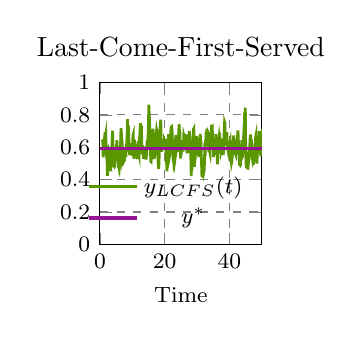
\begin{tikzpicture}
\begin{axis}[
    title=Last-Come-First-Served,
    width=0.3\textwidth,
    height=0.3\textwidth,
    xlabel={Time},
    ymin=0,ymax=1,
    xmin=0,xmax=50,
    grid,
    legend pos=south east
    ]
    \addplot[color=verdecito, solid, line width=1pt]
        table[row sep={\\}]
        {
            \\
            0.8  0.648172716495346  \\
            0.9  0.6228943502894007  \\
            1.0  0.53757384569  \\
            1.1  0.5696338694468187  \\
            1.2  0.586669001687198  \\
            1.3  0.6336557948452597  \\
            1.4  0.6514630912305297  \\
            1.5  0.6714547685744536  \\
            1.6  0.6934264358411159  \\
            1.7  0.6713936205499027  \\
            1.8  0.6825671301588654  \\
            1.9  0.6036251496528495  \\
            2.0  0.567678550382904  \\
            2.1  0.5726124750358232  \\
            2.2  0.5177164958163958  \\
            2.3  0.42320310239767234  \\
            2.4  0.46537877640953473  \\
            2.5  0.4775928900807589  \\
            2.6  0.5176604670887786  \\
            2.7  0.5216268649505467  \\
            2.8  0.5627923219442206  \\
            2.9  0.5536078139583247  \\
            3.0  0.5170781283900148  \\
            3.1  0.5423496302822906  \\
            3.2  0.5317805582693897  \\
            3.3  0.45171955449703693  \\
            3.4  0.5022744555932301  \\
            3.5  0.5197480127240057  \\
            3.6  0.5894137757829543  \\
            3.7  0.6082135846651018  \\
            3.8  0.6699714057150934  \\
            3.9  0.7025402807207253  \\
            4.0  0.6178034123723535  \\
            4.1  0.5918130623846101  \\
            4.2  0.5664302107571997  \\
            4.3  0.4820768398586335  \\
            4.4  0.48011268298848453  \\
            4.5  0.4909036089514949  \\
            4.6  0.48964338925727713  \\
            4.7  0.5210172485091986  \\
            4.8  0.5385223770362115  \\
            4.9  0.5350036444890343  \\
            5.0  0.5425134285036899  \\
            5.1  0.5870231297538195  \\
            5.2  0.6438564829241189  \\
            5.3  0.6116436416332816  \\
            5.4  0.5763478258892087  \\
            5.5  0.5444164900789428  \\
            5.6  0.6085357638050812  \\
            5.7  0.4989735289648598  \\
            5.8  0.5021948875581552  \\
            5.9  0.4859756868832763  \\
            6.0  0.5054767204474979  \\
            6.1  0.49219349684472835  \\
            6.2  0.5139481287531931  \\
            6.3  0.5890086068809088  \\
            6.4  0.6441585753307049  \\
            6.5  0.7176779887699682  \\
            6.6  0.6999838391324271  \\
            6.7  0.6355679700979628  \\
            6.8  0.6404042740694944  \\
            6.9  0.6176588306043591  \\
            7.0  0.5184303325269086  \\
            7.1  0.52592352141642  \\
            7.2  0.5108423445372425  \\
            7.3  0.5537730660918632  \\
            7.4  0.5715234918920533  \\
            7.5  0.524312104840309  \\
            7.6  0.5297458984019698  \\
            7.7  0.5569227844993039  \\
            7.8  0.5502713570076647  \\
            7.9  0.5645037836559652  \\
            8.0  0.5417977248792694  \\
            8.1  0.5768903956955791  \\
            8.2  0.6017448832151704  \\
            8.3  0.639106066141812  \\
            8.4  0.6817575010250501  \\
            8.5  0.7733339964964996  \\
            8.6  0.6726469760726506  \\
            8.7  0.6929602823747949  \\
            8.8  0.7355067593151325  \\
            8.9  0.6589763235514159  \\
            9.0  0.6205254161454565  \\
            9.1  0.5700807321640848  \\
            9.2  0.5506307404497299  \\
            9.3  0.6258851041912656  \\
            9.4  0.5701454727413555  \\
            9.5  0.5684783241025873  \\
            9.6  0.56499350924636  \\
            9.7  0.5622991200857062  \\
            9.8  0.568742942173607  \\
            9.9  0.6033500181296407  \\
            10.0  0.5806462769366902  \\
            10.1  0.6132182658927565  \\
            10.2  0.672967366830763  \\
            10.3  0.6799330690604215  \\
            10.4  0.5623800383001125  \\
            10.5  0.5287120577673896  \\
            10.6  0.5624713284169598  \\
            10.7  0.6471854120545206  \\
            10.8  0.5989637966328374  \\
            10.9  0.5849767108785304  \\
            11.0  0.5768610096662368  \\
            11.1  0.610469287603939  \\
            11.2  0.5737254637633828  \\
            11.3  0.6217726370589745  \\
            11.4  0.5873974708915917  \\
            11.5  0.5667071795367473  \\
            11.6  0.5284820020338685  \\
            11.7  0.5483426179627866  \\
            11.8  0.6040361737642961  \\
            11.9  0.6381390703033833  \\
            12.0  0.5606363664614875  \\
            12.1  0.551303377598316  \\
            12.2  0.6441068864572088  \\
            12.3  0.6729970387931221  \\
            12.4  0.705801948666041  \\
            12.5  0.7486961516868114  \\
            12.6  0.7295049781339085  \\
            12.7  0.7183249491340717  \\
            12.8  0.7336723951858293  \\
            12.9  0.64385825896791  \\
            13.0  0.5631690730045076  \\
            13.1  0.6125064144852903  \\
            13.2  0.5530243685382388  \\
            13.3  0.5893257471631905  \\
            13.4  0.5827011837300589  \\
            13.5  0.5266202493615779  \\
            13.6  0.6052520198942677  \\
            13.7  0.5866074560340415  \\
            13.8  0.5462301177367532  \\
            13.9  0.6049284341493077  \\
            14.0  0.5700800684792817  \\
            14.1  0.5640440003072769  \\
            14.2  0.5238317999892317  \\
            14.3  0.5383633263414502  \\
            14.4  0.5576550470759329  \\
            14.5  0.5905581180926305  \\
            14.6  0.6484088085947626  \\
            14.7  0.6224065635169289  \\
            14.8  0.6349273522672405  \\
            14.9  0.6866573677386647  \\
            15.0  0.7656935288715161  \\
            15.1  0.8625133206940045  \\
            15.2  0.8159185279971801  \\
            15.3  0.7729192259123145  \\
            15.4  0.7244574528229073  \\
            15.5  0.6414221060448533  \\
            15.6  0.5876955049734303  \\
            15.7  0.5116639924625339  \\
            15.8  0.5099075036984573  \\
            15.9  0.5854357652236004  \\
            16.0  0.6033315456958697  \\
            16.1  0.6585460655815076  \\
            16.2  0.6711504718722665  \\
            16.3  0.694624723073737  \\
            16.4  0.7140434372314353  \\
            16.5  0.6710571112319581  \\
            16.6  0.5932819921633836  \\
            16.7  0.6283730820395448  \\
            16.8  0.5269339231664816  \\
            16.9  0.5831681063737477  \\
            17.0  0.5533309611700759  \\
            17.1  0.6061055722081505  \\
            17.2  0.61413910213939  \\
            17.3  0.5790229383179089  \\
            17.4  0.6790229383179067  \\
            17.5  0.7032741622033996  \\
            17.6  0.6914757165627918  \\
            17.7  0.5751064793289942  \\
            17.8  0.5935130149976295  \\
            17.9  0.5403286931760469  \\
            18.0  0.4998107355775545  \\
            18.1  0.4670045590869343  \\
            18.2  0.4857618888183879  \\
            18.3  0.5474622805545231  \\
            18.4  0.6340430989115404  \\
            18.5  0.7081028778035474  \\
            18.6  0.7312261642375191  \\
            18.7  0.7257190534491187  \\
            18.8  0.7699415217365022  \\
            18.9  0.60408619238056  \\
            19.0  0.572285148863326  \\
            19.1  0.6170972820206799  \\
            19.2  0.622990404782918  \\
            19.3  0.6283367364108905  \\
            19.4  0.6497092924924068  \\
            19.5  0.5939483722975041  \\
            19.6  0.6456202544014218  \\
            19.7  0.5980982811892623  \\
            19.8  0.5957847252804029  \\
            19.9  0.641437434396213  \\
            20.0  0.6350315639338397  \\
            20.1  0.6325487499110096  \\
            20.2  0.6425141032413499  \\
            20.3  0.6406181308637464  \\
            20.4  0.5994464215853839  \\
            20.5  0.5201973346869053  \\
            20.6  0.49841172541586687  \\
            20.7  0.45139087938202493  \\
            20.8  0.4933556834840438  \\
            20.9  0.504520850777805  \\
            21.0  0.6045208507778064  \\
            21.1  0.5985628017937152  \\
            21.2  0.680230302636808  \\
            21.3  0.6426098640382492  \\
            21.4  0.6284638070039392  \\
            21.5  0.6349007810261895  \\
            21.6  0.5580399003806136  \\
            21.7  0.5690155958294483  \\
            21.8  0.600337068899691  \\
            21.9  0.7003370688996888  \\
            22.0  0.7241921875317807  \\
            22.1  0.7262490671636641  \\
            22.2  0.6840773067713215  \\
            22.3  0.6876755478228809  \\
            22.4  0.6280901026685868  \\
            22.5  0.6486309612847947  \\
            22.6  0.5340999935248796  \\
            22.7  0.5369444576015532  \\
            22.8  0.507699703347047  \\
            22.9  0.5184403563308884  \\
            23.0  0.5393094247988159  \\
            23.1  0.5147731467475332  \\
            23.2  0.5289170755080193  \\
            23.3  0.5986541895919117  \\
            23.4  0.6763803028339872  \\
            23.5  0.6056772445797804  \\
            23.6  0.5786842610411931  \\
            23.7  0.590196720015328  \\
            23.8  0.5716693590260107  \\
            23.9  0.6522053815936317  \\
            24.0  0.5739174955466879  \\
            24.1  0.5928450292145904  \\
            24.2  0.6374068056252185  \\
            24.3  0.6526466405007909  \\
            24.4  0.7335104574405307  \\
            24.5  0.733608295420531  \\
            24.6  0.6628943587184999  \\
            24.7  0.6950153866762996  \\
            24.8  0.5860903063395213  \\
            24.9  0.5303479971688212  \\
            25.0  0.572022326624289  \\
            25.1  0.5522848508778395  \\
            25.2  0.589516305553559  \\
            25.3  0.5743608178280581  \\
            25.4  0.6432964801016574  \\
            25.5  0.5973631071037495  \\
            25.6  0.5931290815004999  \\
            25.7  0.5729201056727362  \\
            25.8  0.6141651973348594  \\
            25.9  0.6697182730904352  \\
            26.0  0.661630938100263  \\
            26.1  0.6652644379090873  \\
            26.2  0.6570728464482798  \\
            26.3  0.6389445326466294  \\
            26.4  0.596273564504159  \\
            26.5  0.6311320286169284  \\
            26.6  0.6608088122031575  \\
            26.7  0.6796502388442853  \\
            26.8  0.6047274615207705  \\
            26.9  0.5634651923610967  \\
            27.0  0.6423573117506258  \\
            27.1  0.6094411745556982  \\
            27.2  0.6184779587099243  \\
            27.3  0.5643465061574773  \\
            27.4  0.5785419044619466  \\
            27.5  0.6386400573519744  \\
            27.6  0.7003400414639103  \\
            27.7  0.6717765144357131  \\
            27.8  0.6641809089787003  \\
            27.9  0.6285929000866766  \\
            28.0  0.5755882202729872  \\
            28.1  0.513707898494399  \\
            28.2  0.42240453387469756  \\
            28.3  0.4951263520515852  \\
            28.4  0.5103050321799607  \\
            28.5  0.5045339700186418  \\
            28.6  0.5666369283628221  \\
            28.7  0.6015409197354948  \\
            28.8  0.6473748970076336  \\
            28.9  0.7124356317558309  \\
            29.0  0.7162949747870861  \\
            29.1  0.5450667260804565  \\
            29.2  0.47870547765242577  \\
            29.3  0.5505045719107926  \\
            29.4  0.5716402816335346  \\
            29.5  0.5744757483498226  \\
            29.6  0.5829083752013844  \\
            29.7  0.615124514107567  \\
            29.8  0.6147729602074676  \\
            29.9  0.6705593966012486  \\
            30.0  0.6376036839839401  \\
            30.1  0.6035485859028036  \\
            30.2  0.6169003065432292  \\
            30.3  0.6516455332600231  \\
            30.4  0.6053764230210916  \\
            30.5  0.5919857460241431  \\
            30.6  0.5972075894880007  \\
            30.7  0.5396818348093007  \\
            30.8  0.5602874573461101  \\
            30.9  0.6396725538197003  \\
            31.0  0.6826413104756988  \\
            31.1  0.618276919173887  \\
            31.2  0.6412007941056181  \\
            31.3  0.5443884116194333  \\
            31.4  0.48683848874294355  \\
            31.5  0.4169658576216406  \\
            31.6  0.455142525096182  \\
            31.7  0.46782931945652706  \\
            31.8  0.4120430779382893  \\
            31.9  0.45423745702550633  \\
            32.0  0.47311416699544395  \\
            32.1  0.4492617469800244  \\
            32.2  0.4597757287856332  \\
            32.3  0.5168813328058661  \\
            32.4  0.6265065680565165  \\
            32.5  0.5476808599211118  \\
            32.6  0.6470289560883593  \\
            32.7  0.615682898003854  \\
            32.8  0.6969441707504558  \\
            32.9  0.6797215318623628  \\
            33.0  0.7140544842599681  \\
            33.1  0.6863262463264803  \\
            33.2  0.705077988856992  \\
            33.3  0.6669691824252482  \\
            33.4  0.6895999569463598  \\
            33.5  0.6846296051982108  \\
            33.6  0.5683738036981367  \\
            33.7  0.6626901591458108  \\
            33.8  0.5863316427854812  \\
            33.9  0.5745482590953799  \\
            34.0  0.5648370491289896  \\
            34.1  0.646606488990308  \\
            34.2  0.6854113199762963  \\
            34.3  0.6714727240339968  \\
            34.4  0.6874037618053421  \\
            34.5  0.739911927413921  \\
            34.6  0.706100591239263  \\
            34.7  0.7113104306038096  \\
            34.8  0.6562977610491529  \\
            34.9  0.6408866882015403  \\
            35.0  0.6265162058016784  \\
            35.1  0.539927240393304  \\
            35.2  0.6105632705489015  \\
            35.3  0.5915374434806324  \\
            35.4  0.5539606057454662  \\
            35.5  0.579174264273199  \\
            35.6  0.5786786541793063  \\
            35.7  0.6163367575572565  \\
            35.8  0.6806601998168773  \\
            35.9  0.6221444164948693  \\
            36.0  0.6023947501158489  \\
            36.1  0.6217020519309884  \\
            36.2  0.566819468646095  \\
            36.3  0.4947952302967096  \\
            36.4  0.5508563904607797  \\
            36.5  0.5970609460670744  \\
            36.6  0.6622413686816415  \\
            36.7  0.6460735151573544  \\
            36.8  0.6631846747346088  \\
            36.9  0.6440272429658265  \\
            37.0  0.6894029722383905  \\
            37.1  0.5908682984058728  \\
            37.2  0.5897449703496136  \\
            37.3  0.6159895454250801  \\
            37.4  0.5739173764606278  \\
            37.5  0.5823204922786971  \\
            37.6  0.6536634002078543  \\
            37.7  0.6185104461473969  \\
            37.8  0.5513506521011919  \\
            37.9  0.6041131204197399  \\
            38.0  0.6353478578893856  \\
            38.1  0.5521230002104431  \\
            38.2  0.5961656551502017  \\
            38.3  0.6546195115218509  \\
            38.4  0.7052259664988512  \\
            38.5  0.755534383749719  \\
            38.6  0.749581198572173  \\
            38.7  0.6532505807164668  \\
            38.8  0.6518093042622155  \\
            38.9  0.610665256704813  \\
            39.0  0.6276230079617946  \\
            39.1  0.6841876174605943  \\
            39.2  0.6847560483590911  \\
            39.3  0.625575524482997  \\
            39.4  0.5980298067612608  \\
            39.5  0.586280172700711  \\
            39.6  0.6211684985347148  \\
            39.7  0.5942227919873488  \\
            39.8  0.5530173830663117  \\
            39.9  0.5723556758161408  \\
            40.0  0.5871231960513938  \\
            40.1  0.622486741238319  \\
            40.2  0.6321526261185397  \\
            40.3  0.5713088242878186  \\
            40.4  0.5796366409900671  \\
            40.5  0.5273675070470958  \\
            40.6  0.5076589676351091  \\
            40.7  0.519690778368421  \\
            40.8  0.5648730336607954  \\
            40.9  0.5547068466275036  \\
            41.0  0.5798164776629662  \\
            41.1  0.5944289467833457  \\
            41.2  0.6144445123044946  \\
            41.3  0.6723024309725929  \\
            41.4  0.6323278155312835  \\
            41.5  0.6024306326108828  \\
            41.6  0.5881310903111725  \\
            41.7  0.5630527879431142  \\
            41.8  0.5597326254709856  \\
            41.9  0.55493005711363  \\
            42.0  0.6156749601233926  \\
            42.1  0.5956484064008976  \\
            42.2  0.6110908497665406  \\
            42.3  0.6470631996735392  \\
            42.4  0.6494206627740837  \\
            42.5  0.6639218704036978  \\
            42.6  0.7039949078300367  \\
            42.7  0.6734506010279304  \\
            42.8  0.612999470960176  \\
            42.9  0.5611138554373625  \\
            43.0  0.5648056048699317  \\
            43.1  0.49404922070000623  \\
            43.2  0.4917198501787041  \\
            43.3  0.5141540077972451  \\
            43.4  0.485431485561989  \\
            43.5  0.5747267018132973  \\
            43.6  0.5899998589638855  \\
            43.7  0.5814323414222784  \\
            43.8  0.6440341002827026  \\
            43.9  0.5375093539196385  \\
            44.0  0.5411608122306788  \\
            44.1  0.5705470729817037  \\
            44.2  0.5748655848542796  \\
            44.3  0.6203721534321431  \\
            44.4  0.6751798536424474  \\
            44.5  0.724734251885188  \\
            44.6  0.7322749893769753  \\
            44.7  0.8171515839100749  \\
            44.8  0.8003231499507208  \\
            44.9  0.8442452931089264  \\
            45.0  0.6286633126957284  \\
            45.1  0.5043205357031795  \\
            45.2  0.4898364265626469  \\
            45.3  0.471441508714868  \\
            45.4  0.5457339341203991  \\
            45.5  0.5740920880944742  \\
            45.6  0.47091451121620054  \\
            45.7  0.4703766562275078  \\
            45.8  0.4892663610135486  \\
            45.9  0.5156575993918366  \\
            46.0  0.5241228788564882  \\
            46.1  0.5612901213445838  \\
            46.2  0.5750921492128853  \\
            46.3  0.6205517562198821  \\
            46.4  0.6602954305845259  \\
            46.5  0.6785854126818123  \\
            46.6  0.6408641809721303  \\
            46.7  0.5963908268391904  \\
            46.8  0.6480847928641396  \\
            46.9  0.5785154780930171  \\
            47.0  0.5404722965715933  \\
            47.1  0.527993554958023  \\
            47.2  0.5432273376516505  \\
            47.3  0.5553549893321588  \\
            47.4  0.4919666018396285  \\
            47.5  0.5479465550722864  \\
            47.6  0.5308733769227629  \\
            47.7  0.5078976995599049  \\
            47.8  0.5616845018468197  \\
            47.9  0.62117046734582  \\
            48.0  0.621672946203411  \\
            48.1  0.6653335410827665  \\
            48.2  0.6753930941259512  \\
            48.3  0.6168005727736983  \\
            48.4  0.5625392641005007  \\
            48.5  0.49968473518646306  \\
            48.6  0.5642535711631069  \\
            48.7  0.5864175334713053  \\
            48.8  0.5990897034251148  \\
            48.9  0.5759778380263896  \\
            49.0  0.560919818059233  \\
            49.1  0.6148884691658125  \\
            49.2  0.6998162491927076  \\
            49.3  0.5885033614359756  \\
            49.4  0.6015564578085701  \\
            49.5  0.5851347966692515  \\
            49.6  0.5652153059997076  \\
            49.7  0.5449754544425005  \\
            49.8  0.5980708775138055  \\
            49.9  0.6286542650998754  \\
            50.0  0.6661973828557421  \\
            50.1  0.6687243867777255  \\
            50.2  0.7131217340975127  \\
            50.3  0.6707798933132381  \\
            50.4  0.6470056809175588  \\
            50.5  0.70386859662527  \\
            50.6  0.6530825344056623  \\
            50.7  0.630324039713912  \\
            50.8  0.6515782198117606  \\
            50.9  0.5588759880085306  \\
            51.0  0.613812050067402  \\
            51.1  0.6165041655853045  \\
            51.2  0.6502104639411854  \\
            51.3  0.5447903579097257  \\
            51.4  0.5860554069217443  \\
            51.5  0.5357537379558792  \\
            51.6  0.5033377463013693  \\
            51.7  0.4504519966298943  \\
            51.8  0.4886324242989559  \\
            51.9  0.4590962120370037  \\
            52.0  0.45605477998473276  \\
            52.1  0.5212283087688689  \\
            52.2  0.5442135637988628  \\
            52.3  0.5700751840668445  \\
            52.4  0.5928874613951436  \\
            52.5  0.6114288262064491  \\
            52.6  0.6568254014604449  \\
            52.7  0.6802466338404969  \\
            52.8  0.6047326626815064  \\
            52.9  0.5982399931001865  \\
            53.0  0.5699290291245873  \\
            53.1  0.546829722179659  \\
            53.2  0.4942472130925708  \\
            53.3  0.5473922245232927  \\
            53.4  0.5952699735291773  \\
            53.5  0.5730665706589164  \\
            53.6  0.5313722595357717  \\
            53.7  0.5396585570553043  \\
            53.8  0.5584539670575168  \\
            53.9  0.5479921746317657  \\
            54.0  0.5533483402472612  \\
            54.1  0.5857004936769741  \\
            54.2  0.5751914130726519  \\
            54.3  0.5030327671255534  \\
            54.4  0.44862652082134247  \\
            54.5  0.5195284375834603  \\
            54.6  0.5596796026915314  \\
            54.7  0.5513873811828702  \\
            54.8  0.5721386715359174  \\
            54.9  0.5674093771413666  \\
            55.0  0.5873150155404119  \\
            55.1  0.52481435629619  \\
            55.2  0.5449798678159823  \\
            55.3  0.6109200634124576  \\
            55.4  0.5698462611143356  \\
            55.5  0.611286171945018  \\
            55.6  0.6127972349235975  \\
            55.7  0.48555574604949925  \\
            55.8  0.474572526177127  \\
            55.9  0.4991381994377946  \\
            56.0  0.5460326817224868  \\
            56.1  0.565212961730083  \\
            56.2  0.5599471730026693  \\
            56.3  0.6125838353119661  \\
            56.4  0.6707604210897316  \\
            56.5  0.6466238526786867  \\
            56.6  0.7313952217291941  \\
            56.7  0.6670286108502452  \\
            56.8  0.608860903424933  \\
            56.9  0.5756791832295676  \\
            57.0  0.5623131687058205  \\
            57.1  0.5290663943783613  \\
            57.2  0.5558583772034353  \\
            57.3  0.5952883180722708  \\
            57.4  0.6471015398662914  \\
            57.5  0.7026957969146679  \\
            57.6  0.7134195363231939  \\
            57.7  0.7447726037137912  \\
            57.8  0.7712602744920218  \\
            57.9  0.7141871585443482  \\
            58.0  0.6391020983920939  \\
            58.1  0.6285732917252673  \\
            58.2  0.5443754158203902  \\
            58.3  0.594621413716375  \\
            58.4  0.49212546264712387  \\
            58.5  0.5611294169995205  \\
            58.6  0.5724299089259333  \\
            58.7  0.5826075587838773  \\
            58.8  0.5095794168924286  \\
            58.9  0.5976485390701356  \\
            59.0  0.625455158216738  \\
            59.1  0.6249923322179853  \\
            59.2  0.6290598127338356  \\
            59.3  0.654007669475682  \\
            59.4  0.6321189418930473  \\
            59.5  0.6047395418413046  \\
            59.6  0.515678129292013  \\
            59.7  0.5079220242505826  \\
            59.8  0.4801759726859629  \\
            59.9  0.4921450590237768  \\
            60.0  0.5405717549436773  \\
            60.1  0.558295507677073  \\
            60.2  0.6582955076770745  \\
            60.3  0.6514391141851448  \\
            60.4  0.6643596108282779  \\
            60.5  0.6338948982889789  \\
            60.6  0.5832446871081274  \\
            60.7  0.5422185562733404  \\
            60.8  0.46761190496498983  \\
            60.9  0.46251782661578034  \\
            61.0  0.5452609411218816  \\
            61.1  0.563947117111077  \\
            61.2  0.5488849875375976  \\
            61.3  0.5904875433866863  \\
            61.4  0.5729514833438003  \\
            61.5  0.6243439401550575  \\
            61.6  0.651306366855664  \\
            61.7  0.6091707766216317  \\
            61.8  0.5629984307546607  \\
            61.9  0.5610421439451017  \\
            62.0  0.5456512697402829  \\
            62.1  0.48518681030308386  \\
            62.2  0.5284491365744017  \\
            62.3  0.5556705143862217  \\
            62.4  0.6217167931327765  \\
            62.5  0.6399217885258679  \\
            62.6  0.567086658782479  \\
            62.7  0.6211754183980602  \\
            62.8  0.6251159372004338  \\
            62.9  0.6109312416611985  \\
            63.0  0.5139656665964552  \\
            63.1  0.5823026208501005  \\
            63.2  0.6707898162301618  \\
            63.3  0.6220011728208377  \\
            63.4  0.6461845637319712  \\
            63.5  0.7008695567025924  \\
            63.6  0.7459447583361936  \\
            63.7  0.7221081892410552  \\
            63.8  0.6724817516245807  \\
            63.9  0.6231897713314325  \\
            64.0  0.556975345860657  \\
            64.1  0.5687847571386442  \\
            64.2  0.5850705142590797  \\
            64.3  0.5972909469782621  \\
            64.4  0.5523943751657541  \\
            64.5  0.6131413356287325  \\
            64.6  0.6911314100810486  \\
            64.7  0.642205387546781  \\
            64.8  0.6081319436008954  \\
            64.9  0.5724458845313762  \\
            65.0  0.5646644374072167  \\
            65.1  0.4913704552588314  \\
            65.2  0.42916644964087425  \\
            65.3  0.46229762050900547  \\
            65.4  0.45659050650760946  \\
            65.5  0.5170694013684596  \\
            65.6  0.5600554895058139  \\
            65.7  0.6394579826360314  \\
            65.8  0.6623344858410007  \\
            65.9  0.7001684119001794  \\
            66.0  0.6471596185233892  \\
            66.1  0.6244996041417608  \\
            66.2  0.5380818696529701  \\
            66.3  0.522548813419121  \\
            66.4  0.5585259370435551  \\
            66.5  0.5753314595023369  \\
            66.6  0.6272016251823089  \\
            66.7  0.6109876862165606  \\
            66.8  0.6564323256253459  \\
            66.9  0.6391175348756093  \\
            67.0  0.6577379705113913  \\
            67.1  0.6850927639925004  \\
            67.2  0.6011485141830235  \\
            67.3  0.5855573411088244  \\
            67.4  0.5336719268540548  \\
            67.5  0.6095614193549324  \\
            67.6  0.5729329722395136  \\
            67.7  0.5862177974670573  \\
            67.8  0.5876547724339076  \\
            67.9  0.658354828948049  \\
            68.0  0.5972198186442483  \\
            68.1  0.5734967400310893  \\
            68.2  0.5540440873122208  \\
            68.3  0.5841302221514866  \\
            68.4  0.6077147734619075  \\
            68.5  0.577096426842644  \\
            68.6  0.6445470424232411  \\
            68.7  0.6431703563489748  \\
            68.8  0.6716983985180889  \\
            68.9  0.5587303166949056  \\
            69.0  0.6260294142167737  \\
            69.1  0.6391644117238116  \\
            69.2  0.559195545653111  \\
            69.3  0.5535771427969962  \\
            69.4  0.5960833931602991  \\
            69.5  0.6695771870194989  \\
            69.6  0.7492759436326395  \\
            69.7  0.6057992715986558  \\
            69.8  0.6645423386870704  \\
            69.9  0.7089364297895031  \\
            70.0  0.7095044443713476  \\
            70.1  0.6753780219475374  \\
            70.2  0.6696541647292236  \\
            70.3  0.6538338177199563  \\
            70.4  0.6372116453536876  \\
            70.5  0.6804513466956621  \\
            70.6  0.6123527689327517  \\
            70.7  0.5849268076747194  \\
            70.8  0.5768399659554433  \\
            70.9  0.6576455707199216  \\
            71.0  0.5544263302635386  \\
            71.1  0.5190341597892854  \\
            71.2  0.4980987588479451  \\
            71.3  0.5077689378532142  \\
            71.4  0.5127763502466394  \\
            71.5  0.5348637340548947  \\
            71.6  0.6078673947443036  \\
            71.7  0.6148710703143507  \\
            71.8  0.6462110897019784  \\
            71.9  0.6251343425571037  \\
            72.0  0.680838159616485  \\
            72.1  0.6992637133783717  \\
            72.2  0.7181554924709275  \\
            72.3  0.6419530247631968  \\
            72.4  0.5981698060516436  \\
            72.5  0.6149378489139679  \\
            72.6  0.6055824678087163  \\
            72.7  0.5451509027930825  \\
            72.8  0.5174033927249013  \\
            72.9  0.533035629763944  \\
            73.0  0.4787911009370305  \\
            73.1  0.4572894609100615  \\
            73.2  0.5459727280326518  \\
            73.3  0.5673779987803584  \\
            73.4  0.5645925703807251  \\
            73.5  0.6138625245851443  \\
            73.6  0.5889826782587306  \\
            73.7  0.607832896186153  \\
            73.8  0.5477584410665344  \\
            73.9  0.5571311175988001  \\
            74.0  0.6059793297034304  \\
            74.1  0.6573569751281809  \\
            74.2  0.6310641199548286  \\
            74.3  0.6544872897222973  \\
            74.4  0.6025942401079192  \\
            74.5  0.6338338748643224  \\
            74.6  0.5545536137983333  \\
            74.7  0.5717669860912338  \\
            74.8  0.563565798164845  \\
            74.9  0.6073368744196728  \\
            75.0  0.5313173026134592  \\
            75.1  0.5189241798147748  \\
            75.2  0.5548451267214318  \\
            75.3  0.6081810372673147  \\
            75.4  0.7019838680602675  \\
            75.5  0.7011042808307053  \\
            75.6  0.7660733029056672  \\
            75.7  0.7935142171873082  \\
            75.8  0.7770859641589141  \\
            75.9  0.6829901439705139  \\
            76.0  0.6228042947555537  \\
            76.1  0.6240803433278046  \\
            76.2  0.5303165054609025  \\
            76.3  0.5689010736184201  \\
            76.4  0.5603696256354027  \\
            76.5  0.6297509937089814  \\
            76.6  0.6904495756678699  \\
            76.7  0.674316610964425  \\
            76.8  0.7183746677736025  \\
            76.9  0.5449173704326142  \\
            77.0  0.6055108547126054  \\
            77.1  0.6525487548811668  \\
            77.2  0.6851922104463029  \\
            77.3  0.5807301590388079  \\
            77.4  0.5667861177462186  \\
            77.5  0.5948744714321776  \\
            77.6  0.546209807337604  \\
            77.7  0.5269415147492822  \\
            77.8  0.5729767243630448  \\
            77.9  0.5793229975140264  \\
            78.0  0.5822461742178433  \\
            78.1  0.6493017591612471  \\
            78.2  0.7440210264573466  \\
            78.3  0.7615979167401434  \\
            78.4  0.7744866839622517  \\
            78.5  0.6718114458676041  \\
            78.6  0.6491081924252882  \\
            78.7  0.6628091342482918  \\
            78.8  0.5872940250239225  \\
            78.9  0.5642039990941754  \\
            79.0  0.6551235299478435  \\
            79.1  0.6629127612496859  \\
            79.2  0.6267716872180955  \\
            79.3  0.6973408225057938  \\
            79.4  0.5749386807700887  \\
            79.5  0.5657087413940616  \\
            79.6  0.5445664703129438  \\
            79.7  0.5454025323802085  \\
            79.8  0.5580731549493123  \\
            79.9  0.5727902978648416  \\
            80.0  0.6088388010813901  \\
            80.1  0.5736187394784196  \\
            80.2  0.6139210000916222  \\
            80.3  0.5400027687769295  \\
            80.4  0.5878880739563783  \\
            80.5  0.4992362358973139  \\
            80.6  0.5436436984656154  \\
            80.7  0.5084404950275427  \\
            80.8  0.5613819265131781  \\
            80.9  0.5043850195112611  \\
            81.0  0.5622215155804469  \\
            81.1  0.5343087636133532  \\
            81.2  0.5982498875775235  \\
            81.3  0.5091833104633565  \\
            81.4  0.5890673086731084  \\
            81.5  0.6243542148617394  \\
            81.6  0.6368655966380601  \\
            81.7  0.6487645716471349  \\
            81.8  0.7622025398140408  \\
            81.9  0.7686740056297054  \\
            82.0  0.8543555366697149  \\
            82.1  0.6911025600111458  \\
            82.2  0.6489247559924536  \\
            82.3  0.6979962429714561  \\
            82.4  0.7387884162706655  \\
            82.5  0.6737887663629891  \\
            82.6  0.6479404540255302  \\
            82.7  0.6039880401182103  \\
            82.8  0.6220397179893951  \\
            82.9  0.582172933421262  \\
            83.0  0.5217474770974775  \\
            83.1  0.5488565218343808  \\
            83.2  0.5676691430678602  \\
            83.3  0.5608390034874731  \\
            83.4  0.5928720453758416  \\
            83.5  0.5971155489747844  \\
            83.6  0.5791744488652597  \\
            83.7  0.5836336748535729  \\
            83.8  0.5721163324737546  \\
            83.9  0.6345478641663647  \\
            84.0  0.5623258408068494  \\
            84.1  0.5498512746459312  \\
            84.2  0.555325694517407  \\
            84.3  0.5678360155689006  \\
            84.4  0.5515855540785566  \\
            84.5  0.6494057058946794  \\
            84.6  0.5926934629316065  \\
            84.7  0.5822781742181604  \\
            84.8  0.6761926572365553  \\
            84.9  0.664423657994675  \\
            85.0  0.6778257027847587  \\
            85.1  0.5770946836960036  \\
            85.2  0.6388690261210002  \\
            85.3  0.5436296389621873  \\
            85.4  0.6096699919363004  \\
            85.5  0.6453539742905292  \\
            85.6  0.6005518616176602  \\
            85.7  0.6272115950156234  \\
            85.8  0.6598466415201045  \\
            85.9  0.5845232127552151  \\
            86.0  0.5804100648113462  \\
            86.1  0.6503076788144853  \\
            86.2  0.5901662817448141  \\
            86.3  0.49865628722488964  \\
            86.4  0.5712408204249755  \\
            86.5  0.601421390677686  \\
            86.6  0.5010778474124464  \\
            86.7  0.5102386778154511  \\
            86.8  0.5034199820960055  \\
            86.9  0.4893793292653754  \\
            87.0  0.5061768995459204  \\
            87.1  0.50720435475111  \\
            87.2  0.49998793372998307  \\
            87.3  0.5400934610677837  \\
            87.4  0.4841973659896297  \\
            87.5  0.54587652478466  \\
            87.6  0.5719727396943881  \\
            87.7  0.6398126347603181  \\
            87.8  0.6660625818145576  \\
            87.9  0.5802148344377969  \\
            88.0  0.650511679657285  \\
            88.1  0.6072098716047947  \\
            88.2  0.6163048113050849  \\
            88.3  0.5792498406198945  \\
            88.4  0.5838373685807312  \\
            88.5  0.6314413925078242  \\
            88.6  0.567768594856048  \\
            88.7  0.510143264389967  \\
            88.8  0.4880739700087844  \\
            88.9  0.48022353732312695  \\
            89.0  0.5906622882844914  \\
            89.1  0.5169659752754114  \\
            89.2  0.5560047849910745  \\
            89.3  0.5723677178560962  \\
            89.4  0.6220527959900579  \\
            89.5  0.6843044348721605  \\
            89.6  0.7543058801854698  \\
            89.7  0.7103441698227471  \\
            89.8  0.7407511615009241  \\
            89.9  0.7096988404526883  \\
            90.0  0.7200276267617056  \\
            90.1  0.6964201069240517  \\
            90.2  0.6243573415348465  \\
            90.3  0.5685076395457287  \\
            90.4  0.5178199835397379  \\
            90.5  0.5168758935107434  \\
            90.6  0.543872759968977  \\
            90.7  0.5442170565184057  \\
            90.8  0.553223783138165  \\
            90.9  0.5572136433207788  \\
            91.0  0.5788492937735299  \\
            91.1  0.5826284200728082  \\
            91.2  0.58840228708155  \\
            91.3  0.5105903815801582  \\
            91.4  0.5142477731588571  \\
            91.5  0.4554460095460229  \\
            91.6  0.4553565841813878  \\
            91.7  0.47551515962551605  \\
            91.8  0.5145972001519254  \\
            91.9  0.511141741378907  \\
            92.0  0.5258003887380625  \\
            92.1  0.4898121668961153  \\
            92.2  0.5377451381054499  \\
            92.3  0.5084666627628991  \\
            92.4  0.4872573375540128  \\
            92.5  0.4790612045355829  \\
            92.6  0.5294533696981176  \\
            92.7  0.5948589592300522  \\
            92.8  0.5587703610349593  \\
            92.9  0.5514152841817292  \\
            93.0  0.6137855068926541  \\
            93.1  0.6801037412278106  \\
            93.2  0.7229720978390901  \\
            93.3  0.7213509011376971  \\
            93.4  0.6052240051523938  \\
            93.5  0.5081459162314701  \\
            93.6  0.3899111405564213  \\
            93.7  0.37281347531043707  \\
            93.8  0.40057302603284484  \\
            93.9  0.4346161132337585  \\
            94.0  0.47263432081138035  \\
            94.1  0.5418106076315468  \\
            94.2  0.5472924726386879  \\
            94.3  0.6342519231616564  \\
            94.4  0.7003466992715346  \\
            94.5  0.7305434364612466  \\
            94.6  0.793434368827775  \\
            94.7  0.7436002486992663  \\
            94.8  0.7260994367714062  \\
            94.9  0.7673084162515522  \\
            95.0  0.71489366816634  \\
            95.1  0.6570850014752807  \\
            95.2  0.693223146016436  \\
            95.3  0.7214340923281526  \\
            95.4  0.6901863919363933  \\
            95.5  0.7082163173997174  \\
            95.6  0.6095207611542293  \\
            95.7  0.635603285241416  \\
            95.8  0.6364253623266336  \\
            95.9  0.6560420491729104  \\
            96.0  0.6825219717190549  \\
            96.1  0.6391314994754254  \\
            96.2  0.6860493246894492  \\
            96.3  0.7031030942274299  \\
            96.4  0.6993092265390004  \\
            96.5  0.7685089687776525  \\
            96.6  0.763300045666071  \\
            96.7  0.8311888362656106  \\
            96.8  0.7785650748022448  \\
            96.9  0.6516461197745684  \\
            97.0  0.6907162972238865  \\
            97.1  0.7126856044925205  \\
            97.2  0.5201089764377258  \\
            97.3  0.5683123038586047  \\
            97.4  0.6694887732970756  \\
            97.5  0.6287395835149425  \\
            97.6  0.7102741599172049  \\
            97.7  0.6813328822602216  \\
            97.8  0.6140315777659566  \\
            97.9  0.5673605134549291  \\
            98.0  0.6032225791312982  \\
            98.1  0.5959829691029057  \\
            98.2  0.5846604147629506  \\
            98.3  0.6570985312349222  \\
            98.4  0.5841212736055326  \\
            98.5  0.5868986020855402  \\
            98.6  0.5825346949364842  \\
            98.7  0.5591406347708556  \\
            98.8  0.530856711268413  \\
            98.9  0.5533086961512055  \\
            99.0  0.5293470096465853  \\
            99.1  0.5483568564331307  \\
            99.2  0.5638467731943138  \\
            99.3  0.5404875072303241  \\
            99.4  0.6247707544313243  \\
            99.5  0.6595082523052582  \\
            99.6  0.6793446569718213  \\
            99.7  0.7086049170132611  \\
            99.8  0.7133173315810382  \\
            99.9  0.7839507423541789  \\
            100.0  0.7430086138742809  \\
        }
        ;
    \addlegendentry {$y_{LCFS}(t)$}
    \addplot[color=violetita, solid, very thick]
        table[row sep={\\}]
        {
            \\
            -109.0  0.593  \\
            209.0  0.593  \\
        }
        ;
    \addlegendentry {$y^*$}
\end{axis}
\end{tikzpicture}
    
	\end{center}

\end{frame}

\begin{frame}{Attained work empirical CDF}

	\begin{center}
    \tikzsetnextfilename{lognormal_attained_comparison}
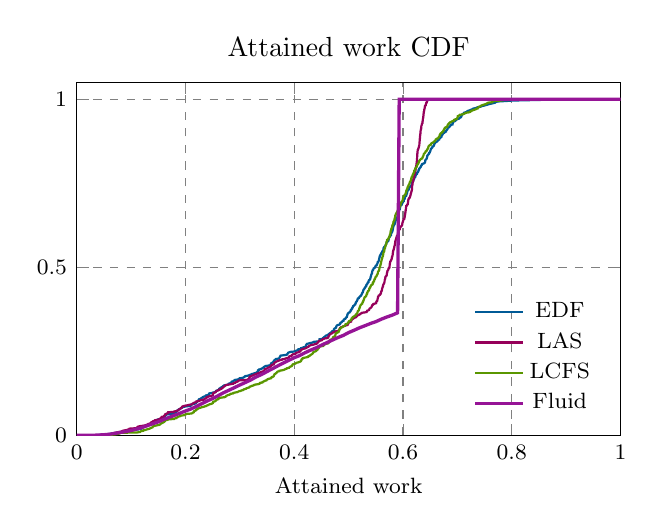
\begin{tikzpicture}
    \begin{axis}[
    title=Attained work CDF,
    width=0.7\textwidth,
    height=0.5\textwidth,
    xlabel={Attained work},
    xmin=0,xmax=1.0,
    ymin=0,ymax=1.05,
    grid,
    legend pos=south east,
    ]
    \addplot[color=azulcito, solid, thick]
        table[row sep={\\}]
        {
            \\
            0.03999952573825993  0.0012484394506866417  \\
            0.050904152061526986  0.0024968789013732834  \\
            0.0582906664795253  0.003745318352059925  \\
            0.06443780317329129  0.004993757802746567  \\
            0.06526949557664707  0.006242197253433208  \\
            0.0725058680007352  0.00749063670411985  \\
            0.07631375012922557  0.008739076154806492  \\
            0.0831567816878845  0.009987515605493134  \\
            0.09022009698995248  0.011235955056179775  \\
            0.09138995224262914  0.012484394506866416  \\
            0.09301695037398616  0.01373283395755306  \\
            0.09778417593471433  0.0149812734082397  \\
            0.10645793977575835  0.016229712858926344  \\
            0.11321331358239917  0.017478152309612985  \\
            0.11460772510761075  0.018726591760299626  \\
            0.11929848887809981  0.019975031210986267  \\
            0.11963819962854672  0.02122347066167291  \\
            0.1204040086064605  0.02247191011235955  \\
            0.1225446567662658  0.02372034956304619  \\
            0.1229620151854591  0.024968789013732832  \\
            0.1245795744844764  0.026217228464419477  \\
            0.12650028746211905  0.02746566791510612  \\
            0.12675288182438038  0.02871410736579276  \\
            0.12888548286638013  0.0299625468164794  \\
            0.134204367554716  0.031210986267166042  \\
            0.13676935071912055  0.03245942571785269  \\
            0.1370163255962956  0.033707865168539325  \\
            0.13746689315698749  0.03495630461922597  \\
            0.138470809089295  0.03620474406991261  \\
            0.13914297931524364  0.03745318352059925  \\
            0.13964231312889447  0.03870162297128589  \\
            0.13973892795121487  0.039950062421972535  \\
            0.14162094017434157  0.04119850187265917  \\
            0.14236671923302033  0.04244694132334582  \\
            0.14501842886009797  0.04369538077403246  \\
            0.14787347552360017  0.0449438202247191  \\
            0.14798564565585176  0.046192259675405745  \\
            0.14920312932845647  0.04744069912609238  \\
            0.15551618725091032  0.04868913857677903  \\
            0.1574254648250371  0.049937578027465665  \\
            0.15891767574800753  0.05118601747815231  \\
            0.15947334190614998  0.052434456928838954  \\
            0.16043399742982864  0.05368289637952559  \\
            0.1622114091740059  0.05493133583021224  \\
            0.1625377423242753  0.056179775280898875  \\
            0.16260962158966288  0.05742821473158552  \\
            0.1627635193972766  0.05867665418227216  \\
            0.16379106023952733  0.0599250936329588  \\
            0.1641392527700134  0.06117353308364544  \\
            0.16662229408462073  0.062421972534332085  \\
            0.17746207169068384  0.06367041198501873  \\
            0.17796591309133  0.06491885143570537  \\
            0.1810287972278246  0.066167290886392  \\
            0.18152198031452713  0.06741573033707865  \\
            0.1825516839976794  0.0686641697877653  \\
            0.18298583669378954  0.06991260923845194  \\
            0.1835243011429695  0.07116104868913857  \\
            0.18398430087826512  0.07240948813982521  \\
            0.1844732088620233  0.07365792759051186  \\
            0.18642836077967684  0.0749063670411985  \\
            0.18707192344476908  0.07615480649188515  \\
            0.1876289674164795  0.07740324594257178  \\
            0.19052872493345227  0.07865168539325842  \\
            0.1910405220781115  0.07990012484394507  \\
            0.191808612930366  0.08114856429463171  \\
            0.1939677692613089  0.08239700374531835  \\
            0.19480796388843233  0.08364544319600499  \\
            0.19728177457563598  0.08489388264669163  \\
            0.20087855775756935  0.08614232209737828  \\
            0.20764375950248848  0.08739076154806492  \\
            0.20999898248710422  0.08863920099875156  \\
            0.21068684862539988  0.0898876404494382  \\
            0.21074553876449897  0.09113607990012484  \\
            0.2121204232091258  0.09238451935081149  \\
            0.21642942368910273  0.09363295880149813  \\
            0.21802170699783424  0.09488139825218476  \\
            0.21937434563267774  0.09612983770287141  \\
            0.2196383277986449  0.09737827715355805  \\
            0.22040664071406305  0.0986267166042447  \\
            0.2216560332589263  0.09987515605493133  \\
            0.22177508517732747  0.10112359550561797  \\
            0.2231504368415956  0.10237203495630462  \\
            0.22343988462377246  0.10362047440699126  \\
            0.22383275342629272  0.10486891385767791  \\
            0.2246479004663655  0.10611735330836454  \\
            0.22483658395623252  0.10736579275905118  \\
            0.2272926898667577  0.10861423220973783  \\
            0.2288157271042459  0.10986267166042447  \\
            0.22934284463366694  0.1111111111111111  \\
            0.231262220380259  0.11235955056179775  \\
            0.23196598989143294  0.1136079900124844  \\
            0.2334957437800469  0.11485642946317104  \\
            0.23604050025786408  0.11610486891385768  \\
            0.2373688383320669  0.11735330836454431  \\
            0.23758659976967955  0.11860174781523096  \\
            0.24151670953310309  0.1198501872659176  \\
            0.2420340885595744  0.12109862671660425  \\
            0.2430319855014214  0.12234706616729088  \\
            0.24373642052213798  0.12359550561797752  \\
            0.24386944005228026  0.12484394506866417  \\
            0.2486376427210009  0.12609238451935081  \\
            0.25069375755875006  0.12734082397003746  \\
            0.25427696798605837  0.1285892634207241  \\
            0.2555258673961172  0.12983770287141075  \\
            0.2558757664082094  0.13108614232209737  \\
            0.2563534655760881  0.132334581772784  \\
            0.2582598074158827  0.13358302122347065  \\
            0.2597452301947597  0.1348314606741573  \\
            0.2616583784359597  0.13607990012484394  \\
            0.2617635275396638  0.1373283395755306  \\
            0.26196152741205486  0.13857677902621723  \\
            0.26323050517396  0.13982521847690388  \\
            0.2650289412038873  0.14107365792759052  \\
            0.2652127354361622  0.14232209737827714  \\
            0.267229165317702  0.14357053682896379  \\
            0.26790202700267685  0.14481897627965043  \\
            0.26871303958494874  0.14606741573033707  \\
            0.27032105652553895  0.14731585518102372  \\
            0.2710568113661509  0.14856429463171036  \\
            0.27528311225967866  0.149812734082397  \\
            0.27813876129221526  0.15106117353308365  \\
            0.2793205112764294  0.1523096129837703  \\
            0.27942057650218466  0.15355805243445692  \\
            0.2816987534937212  0.15480649188514356  \\
            0.28285315430728775  0.1560549313358302  \\
            0.2847438708683796  0.15730337078651685  \\
            0.2847619577800955  0.1585518102372035  \\
            0.28501722651311057  0.15980024968789014  \\
            0.28793734958669054  0.16104868913857678  \\
            0.2884899654926648  0.16229712858926343  \\
            0.29023290284726144  0.16354556803995007  \\
            0.2905387649963309  0.1647940074906367  \\
            0.295671210029127  0.16604244694132334  \\
            0.29788044257681184  0.16729088639200998  \\
            0.2994879158732904  0.16853932584269662  \\
            0.29962010632198144  0.16978776529338327  \\
            0.3051640017711007  0.17103620474406991  \\
            0.3064318418237981  0.17228464419475656  \\
            0.30849173764095633  0.1735330836454432  \\
            0.3087595145433035  0.17478152309612985  \\
            0.30966638504431365  0.1760299625468165  \\
            0.3141952684203478  0.1772784019975031  \\
            0.3169196740422974  0.17852684144818975  \\
            0.3181683618542945  0.1797752808988764  \\
            0.3208523851449445  0.18102372034956304  \\
            0.3215162592536238  0.1822721598002497  \\
            0.32510907107664627  0.18352059925093633  \\
            0.3267295080512369  0.18476903870162298  \\
            0.3299836061494048  0.18601747815230962  \\
            0.3308545815631731  0.18726591760299627  \\
            0.331720143786122  0.18851435705368288  \\
            0.33242747179527093  0.18976279650436953  \\
            0.3331779639045216  0.19101123595505617  \\
            0.33323492984383307  0.19225967540574282  \\
            0.3333535865305065  0.19350811485642946  \\
            0.3351878928767645  0.1947565543071161  \\
            0.33541175959123926  0.19600499375780275  \\
            0.3393095958203656  0.1972534332084894  \\
            0.339743288736301  0.19850187265917604  \\
            0.3417032863063483  0.19975031210986266  \\
            0.342562850582025  0.2009987515605493  \\
            0.3434144515717807  0.20224719101123595  \\
            0.3442726566139282  0.2034956304619226  \\
            0.34573008023447444  0.20474406991260924  \\
            0.34670448074927396  0.20599250936329588  \\
            0.35112605638312017  0.20724094881398253  \\
            0.35564338274821244  0.20848938826466917  \\
            0.35604509953113045  0.20973782771535582  \\
            0.3569342359500822  0.21098626716604243  \\
            0.3569434881816562  0.21223470661672908  \\
            0.3570223320502919  0.21348314606741572  \\
            0.3580101602263783  0.21473158551810237  \\
            0.35947252917988237  0.21598002496878901  \\
            0.3604862459217485  0.21722846441947566  \\
            0.3622230351464113  0.2184769038701623  \\
            0.36225993760795916  0.21972534332084895  \\
            0.36233467544885656  0.2209737827715356  \\
            0.3627168003671245  0.2222222222222222  \\
            0.36366083763143564  0.22347066167290885  \\
            0.36434455654540443  0.2247191011235955  \\
            0.3658446908201812  0.22596754057428214  \\
            0.36645724409341107  0.2272159800249688  \\
            0.37174192324852956  0.22846441947565543  \\
            0.37257211689316183  0.22971285892634208  \\
            0.37268928071353  0.23096129837702872  \\
            0.3729312299383585  0.23220973782771537  \\
            0.37377005092680804  0.23345817727840198  \\
            0.37409626940296903  0.23470661672908863  \\
            0.37433124534782336  0.23595505617977527  \\
            0.3749768345600617  0.23720349563046192  \\
            0.3807030401485061  0.23845193508114856  \\
            0.38601450315041147  0.2397003745318352  \\
            0.38648056449031176  0.24094881398252185  \\
            0.3874946034307134  0.2421972534332085  \\
            0.38816645465106003  0.24344569288389514  \\
            0.38843077925352165  0.24469413233458176  \\
            0.38900756111533485  0.2459425717852684  \\
            0.3908805052292177  0.24719101123595505  \\
            0.3936846783111565  0.2484394506866417  \\
            0.4018455022216292  0.24968789013732834  \\
            0.40230486013553346  0.250936329588015  \\
            0.4040382236733891  0.25218476903870163  \\
            0.40657773211434295  0.2534332084893883  \\
            0.4071488727431575  0.2546816479400749  \\
            0.4073057750030981  0.25593008739076156  \\
            0.4112957671006043  0.2571785268414482  \\
            0.41281590556619807  0.25842696629213485  \\
            0.4128997247109892  0.2596754057428215  \\
            0.41683949779029744  0.26092384519350814  \\
            0.4170055746571961  0.26217228464419473  \\
            0.42079348617122037  0.2634207240948814  \\
            0.42134226267573655  0.264669163545568  \\
            0.4214686960691232  0.26591760299625467  \\
            0.4215054848813937  0.2671660424469413  \\
            0.42165553318409366  0.26841448189762795  \\
            0.422107085626255  0.2696629213483146  \\
            0.42284371965031664  0.27091136079900124  \\
            0.42335872837235655  0.2721598002496879  \\
            0.42680838736318083  0.27340823970037453  \\
            0.42905984554072774  0.2746566791510612  \\
            0.4332800858901672  0.2759051186017478  \\
            0.4350699811584633  0.27715355805243447  \\
            0.43632866789426206  0.2784019975031211  \\
            0.4445677798361982  0.27965043695380776  \\
            0.4453764698861079  0.2808988764044944  \\
            0.44597263073276117  0.28214731585518105  \\
            0.4464231348808411  0.2833957553058677  \\
            0.4465608235513574  0.2846441947565543  \\
            0.4465654794745567  0.2858926342072409  \\
            0.4517468266822554  0.28714107365792757  \\
            0.4523874306854765  0.2883895131086142  \\
            0.45293085466676086  0.28963795255930086  \\
            0.45479211174675527  0.2908863920099875  \\
            0.45484653229366145  0.29213483146067415  \\
            0.4558779788525733  0.2933832709113608  \\
            0.4570605235644223  0.29463171036204744  \\
            0.4575762941656966  0.2958801498127341  \\
            0.4588166822584654  0.29712858926342073  \\
            0.46142012892157425  0.2983770287141074  \\
            0.4619363163997008  0.299625468164794  \\
            0.46347409672682  0.30087390761548066  \\
            0.4642561551541602  0.3021223470661673  \\
            0.46516617148154454  0.30337078651685395  \\
            0.4660838749265208  0.3046192259675406  \\
            0.46717459678603035  0.30586766541822724  \\
            0.4684169107728924  0.30711610486891383  \\
            0.46977563568638536  0.3083645443196005  \\
            0.46988052803046554  0.3096129837702871  \\
            0.4718708067593582  0.31086142322097376  \\
            0.47258970535551725  0.3121098626716604  \\
            0.47265220182060874  0.31335830212234705  \\
            0.47298746998093955  0.3146067415730337  \\
            0.4729983283960877  0.31585518102372034  \\
            0.47362388580447135  0.317103620474407  \\
            0.47457323632337767  0.31835205992509363  \\
            0.4763496582948804  0.3196004993757803  \\
            0.47686396385935825  0.3208489388264669  \\
            0.4770742476445091  0.32209737827715357  \\
            0.47707660023394594  0.3233458177278402  \\
            0.47749954635443165  0.32459425717852686  \\
            0.4777916180417605  0.3258426966292135  \\
            0.47852092747957187  0.32709113607990015  \\
            0.4801749088866889  0.3283395755305868  \\
            0.4829355557507  0.3295880149812734  \\
            0.4842731855568946  0.33083645443196  \\
            0.48441593726884247  0.33208489388264667  \\
            0.484643618393949  0.3333333333333333  \\
            0.48481444436979665  0.33458177278401996  \\
            0.4860416572551074  0.3358302122347066  \\
            0.48743332838356923  0.33707865168539325  \\
            0.4877098471520618  0.3383270911360799  \\
            0.48853343709897756  0.33957553058676654  \\
            0.49044908266085696  0.3408239700374532  \\
            0.4904828001243189  0.34207240948813983  \\
            0.4907472666245193  0.3433208489388265  \\
            0.4912661907919613  0.3445692883895131  \\
            0.4923886551940401  0.34581772784019976  \\
            0.4941085638095615  0.3470661672908864  \\
            0.49462664733919315  0.34831460674157305  \\
            0.49478596399223185  0.3495630461922597  \\
            0.4953273687536618  0.35081148564294634  \\
            0.4967608005476656  0.352059925093633  \\
            0.49686688867705675  0.3533083645443196  \\
            0.4972150154328081  0.3545568039950062  \\
            0.49724396433582263  0.35580524344569286  \\
            0.4974072222170527  0.3570536828963795  \\
            0.49757524294210165  0.35830212234706615  \\
            0.4980387430239547  0.3595505617977528  \\
            0.498233582005353  0.36079900124843944  \\
            0.49837858180819716  0.3620474406991261  \\
            0.4992826648226254  0.36329588014981273  \\
            0.49980626179652177  0.3645443196004994  \\
            0.5018985307811192  0.365792759051186  \\
            0.5020339165561547  0.36704119850187267  \\
            0.5028161525137307  0.3682896379525593  \\
            0.5036720474946925  0.36953807740324596  \\
            0.5037322423532231  0.3707865168539326  \\
            0.5037438726293074  0.37203495630461925  \\
            0.5044529582064435  0.3732833957553059  \\
            0.5054415011161562  0.37453183520599254  \\
            0.5056111586108811  0.3757802746566791  \\
            0.5065981359211094  0.37702871410736577  \\
            0.5066836989841034  0.3782771535580524  \\
            0.5067193358876241  0.37952559300873906  \\
            0.5074933532661272  0.3807740324594257  \\
            0.5077258345746856  0.38202247191011235  \\
            0.5080914550245472  0.383270911360799  \\
            0.5083738895194516  0.38451935081148564  \\
            0.5096479366191846  0.3857677902621723  \\
            0.5105461286151503  0.38701622971285893  \\
            0.5107953692987908  0.3882646691635456  \\
            0.5122904995975427  0.3895131086142322  \\
            0.5123816526508616  0.39076154806491886  \\
            0.5126619955571174  0.3920099875156055  \\
            0.5129882767278389  0.39325842696629215  \\
            0.5130881712436908  0.3945068664169788  \\
            0.5132654505230648  0.39575530586766544  \\
            0.5140270895448397  0.3970037453183521  \\
            0.5147435159653608  0.3982521847690387  \\
            0.5150953169229098  0.3995006242197253  \\
            0.5153172929635478  0.40074906367041196  \\
            0.5160429129774221  0.4019975031210986  \\
            0.5161650980723351  0.40324594257178525  \\
            0.5164769368279278  0.4044943820224719  \\
            0.5167322990003675  0.40574282147315854  \\
            0.5168490869059923  0.4069912609238452  \\
            0.518672946813382  0.40823970037453183  \\
            0.5188543378628632  0.4094881398252185  \\
            0.5196501288580536  0.4107365792759051  \\
            0.5199399531943123  0.41198501872659177  \\
            0.5207593560394166  0.4132334581772784  \\
            0.5220049228309875  0.41448189762796506  \\
            0.522192883639816  0.4157303370786517  \\
            0.5233374961834765  0.41697877652933835  \\
            0.523522285619464  0.418227215980025  \\
            0.5239972909632231  0.41947565543071164  \\
            0.5242916719312092  0.4207240948813982  \\
            0.5244025167235904  0.42197253433208487  \\
            0.5247715184824395  0.4232209737827715  \\
            0.5254733535201908  0.42446941323345816  \\
            0.5259850872894112  0.4257178526841448  \\
            0.5261111509184389  0.42696629213483145  \\
            0.5265751522712208  0.4282147315855181  \\
            0.5267163078307107  0.42946317103620474  \\
            0.5268013503019375  0.4307116104868914  \\
            0.5272037002396104  0.43196004993757803  \\
            0.5273287233331416  0.4332084893882647  \\
            0.5283323455853831  0.4344569288389513  \\
            0.528760925221476  0.43570536828963796  \\
            0.5288870998040678  0.4369538077403246  \\
            0.5295439570865108  0.43820224719101125  \\
            0.5301408373614935  0.4394506866416979  \\
            0.5306356531082379  0.44069912609238454  \\
            0.5308041208415883  0.4419475655430712  \\
            0.5317343720642876  0.4431960049937578  \\
            0.532482498357254  0.4444444444444444  \\
            0.5324835440744096  0.44569288389513106  \\
            0.5325161298621452  0.4469413233458177  \\
            0.5328130488130357  0.44818976279650435  \\
            0.5336866190790633  0.449438202247191  \\
            0.5342626679770179  0.45068664169787764  \\
            0.5345135595374162  0.4519350811485643  \\
            0.5350569870332755  0.45318352059925093  \\
            0.5351755769473239  0.4544319600499376  \\
            0.5364991282384255  0.4556803995006242  \\
            0.5365741612700391  0.45692883895131087  \\
            0.5366594794448218  0.4581772784019975  \\
            0.5368282147832004  0.45942571785268416  \\
            0.5370114548604086  0.4606741573033708  \\
            0.537568353684108  0.46192259675405745  \\
            0.5389046463793009  0.4631710362047441  \\
            0.5395355541755222  0.46441947565543074  \\
            0.539773695136397  0.4656679151061174  \\
            0.5399142740970541  0.46691635455680397  \\
            0.5401420454337684  0.4681647940074906  \\
            0.5401733669204958  0.46941323345817726  \\
            0.5402826099008988  0.4706616729088639  \\
            0.5409311838478685  0.47191011235955055  \\
            0.5409482434909294  0.4731585518102372  \\
            0.5412032469895394  0.47440699126092384  \\
            0.5413038283945735  0.4756554307116105  \\
            0.5413833674685121  0.4769038701622971  \\
            0.5418816017558168  0.4781523096129838  \\
            0.5421771963960484  0.4794007490636704  \\
            0.5423242237357258  0.48064918851435706  \\
            0.5428543637385127  0.4818976279650437  \\
            0.5428808100312228  0.48314606741573035  \\
            0.5429282038000594  0.484394506866417  \\
            0.5431167965174044  0.48564294631710364  \\
            0.5432531859604381  0.4868913857677903  \\
            0.5436430878821943  0.48813982521847693  \\
            0.5437771492273638  0.4893882646691635  \\
            0.5438531756605163  0.49063670411985016  \\
            0.544784467003282  0.4918851435705368  \\
            0.5454171594371787  0.49313358302122345  \\
            0.5454855381919113  0.4943820224719101  \\
            0.5457363754075661  0.49563046192259674  \\
            0.5460604463497027  0.4968789013732834  \\
            0.5469673929668134  0.49812734082397003  \\
            0.5486524691837213  0.4993757802746567  \\
            0.5489654279803664  0.5006242197253433  \\
            0.5491071869595883  0.50187265917603  \\
            0.5491763052482914  0.5031210986267166  \\
            0.5497597409662909  0.5043695380774033  \\
            0.5513416532980598  0.5056179775280899  \\
            0.5517561736107846  0.5068664169787765  \\
            0.5517632853293819  0.5081148564294632  \\
            0.5521288538496236  0.5093632958801498  \\
            0.5529106695491333  0.5106117353308365  \\
            0.5531263462031478  0.5118601747815231  \\
            0.5531654660312293  0.5131086142322098  \\
            0.5534480835724054  0.5143570536828964  \\
            0.553483724918677  0.5156054931335831  \\
            0.5545315705746175  0.5168539325842697  \\
            0.5550299900021258  0.5181023720349563  \\
            0.5551246657284774  0.519350811485643  \\
            0.5555179077636436  0.5205992509363296  \\
            0.5556116016185656  0.5218476903870163  \\
            0.5556314877721031  0.5230961298377028  \\
            0.5559178792832355  0.5243445692883895  \\
            0.5562895686173022  0.5255930087390761  \\
            0.5563911852700442  0.5268414481897628  \\
            0.5566033134683381  0.5280898876404494  \\
            0.5567248848454791  0.529338327091136  \\
            0.5568450087736565  0.5305867665418227  \\
            0.5574030155950993  0.5318352059925093  \\
            0.5574150685334355  0.533083645443196  \\
            0.5577442822797727  0.5343320848938826  \\
            0.5578731054180786  0.5355805243445693  \\
            0.5587192646508612  0.5368289637952559  \\
            0.5590143640544452  0.5380774032459426  \\
            0.5594246443392948  0.5393258426966292  \\
            0.5595981623736006  0.5405742821473158  \\
            0.5599886825492033  0.5418227215980025  \\
            0.5608742752114906  0.5430711610486891  \\
            0.5613965761922515  0.5443196004993758  \\
            0.5614549567375204  0.5455680399500624  \\
            0.5620121968847576  0.5468164794007491  \\
            0.5620682221461286  0.5480649188514357  \\
            0.5632830004248676  0.5493133583021224  \\
            0.5635983636055653  0.550561797752809  \\
            0.5637892776882718  0.5518102372034956  \\
            0.5638921951231948  0.5530586766541823  \\
            0.5639825267607604  0.5543071161048689  \\
            0.5640143331532171  0.5555555555555556  \\
            0.5641421645758837  0.5568039950062422  \\
            0.5649499983584114  0.5580524344569289  \\
            0.565330811294217  0.5593008739076155  \\
            0.5654156752840223  0.5605493133583022  \\
            0.5666204490518183  0.5617977528089888  \\
            0.5667975460556068  0.5630461922596754  \\
            0.5674970099171879  0.5642946317103621  \\
            0.5681660301762149  0.5655430711610487  \\
            0.5681746189343063  0.5667915106117354  \\
            0.5685513589694704  0.568039950062422  \\
            0.5691095916177202  0.5692883895131086  \\
            0.569295180766971  0.5705368289637952  \\
            0.569497052671853  0.5717852684144819  \\
            0.5695331780768953  0.5730337078651685  \\
            0.5704242356927514  0.5742821473158551  \\
            0.5706666049394347  0.5755305867665418  \\
            0.5719039546102916  0.5767790262172284  \\
            0.5727516889312486  0.5780274656679151  \\
            0.5731771900858512  0.5792759051186017  \\
            0.5731867856477497  0.5805243445692884  \\
            0.5735003008793579  0.581772784019975  \\
            0.5735011428181438  0.5830212234706617  \\
            0.573968606840197  0.5842696629213483  \\
            0.5740038805643048  0.5855181023720349  \\
            0.5741920043964017  0.5867665418227216  \\
            0.5744736674883979  0.5880149812734082  \\
            0.5746210786121535  0.5892634207240949  \\
            0.5755576171753143  0.5905118601747815  \\
            0.5759413177373878  0.5917602996254682  \\
            0.5759587961886372  0.5930087390761548  \\
            0.5767886027848013  0.5942571785268415  \\
            0.5778991914876456  0.5955056179775281  \\
            0.5779008581954646  0.5967540574282147  \\
            0.5780451221867081  0.5980024968789014  \\
            0.578089972054897  0.599250936329588  \\
            0.5781843868661555  0.6004993757802747  \\
            0.5786897047327411  0.6017478152309613  \\
            0.5787751360793547  0.602996254681648  \\
            0.5797448913186654  0.6042446941323346  \\
            0.5798033572246657  0.6054931335830213  \\
            0.5801071724515698  0.6067415730337079  \\
            0.5805316625085415  0.6079900124843945  \\
            0.5807539226346854  0.6092384519350812  \\
            0.5808317822643048  0.6104868913857678  \\
            0.581130996506587  0.6117353308364545  \\
            0.5812072712304504  0.6129837702871411  \\
            0.581410547161334  0.6142322097378277  \\
            0.5816411452351244  0.6154806491885143  \\
            0.5816464911772306  0.616729088639201  \\
            0.5818241954601495  0.6179775280898876  \\
            0.5819770339558801  0.6192259675405742  \\
            0.5822296006500665  0.6204744069912609  \\
            0.5824161611342134  0.6217228464419475  \\
            0.5824511133275794  0.6229712858926342  \\
            0.5827665218024123  0.6242197253433208  \\
            0.5834263049711553  0.6254681647940075  \\
            0.5840156187942563  0.6267166042446941  \\
            0.5843237638759076  0.6279650436953808  \\
            0.5847822308483451  0.6292134831460674  \\
            0.5848754781833829  0.630461922596754  \\
            0.5851151506566126  0.6317103620474407  \\
            0.5853369565230797  0.6329588014981273  \\
            0.5858160232765233  0.634207240948814  \\
            0.5858736198788501  0.6354556803995006  \\
            0.5859316098205201  0.6367041198501873  \\
            0.5861346022805525  0.6379525593008739  \\
            0.586849561165053  0.6392009987515606  \\
            0.5871128791526842  0.6404494382022472  \\
            0.5881586984296447  0.6416978776529338  \\
            0.5883745104868154  0.6429463171036205  \\
            0.5884956302839586  0.6441947565543071  \\
            0.5888344306962414  0.6454431960049938  \\
            0.5894610101590552  0.6466916354556804  \\
            0.5895304862243073  0.6479400749063671  \\
            0.5895369887645616  0.6491885143570537  \\
            0.5896340129566939  0.6504369538077404  \\
            0.589778605361901  0.651685393258427  \\
            0.5903707817097296  0.6529338327091136  \\
            0.5904654916943817  0.6541822721598003  \\
            0.590483311678323  0.6554307116104869  \\
            0.5906485240142839  0.6566791510611736  \\
            0.5908089435889963  0.6579275905118602  \\
            0.5911530275819956  0.6591760299625468  \\
            0.5911586962910249  0.6604244694132334  \\
            0.5914228175090477  0.66167290886392  \\
            0.5917501710115702  0.6629213483146067  \\
            0.5919097034973806  0.6641697877652933  \\
            0.5922287740788355  0.66541822721598  \\
            0.5924337065352883  0.6666666666666666  \\
            0.5925887045162019  0.6679151061173533  \\
            0.5927271734975135  0.6691635455680399  \\
            0.5931798110109046  0.6704119850187266  \\
            0.5933886402344866  0.6716604244694132  \\
            0.5941546233478565  0.6729088639200999  \\
            0.5942244854310557  0.6741573033707865  \\
            0.5943544030907416  0.6754057428214731  \\
            0.5944398872925984  0.6766541822721598  \\
            0.5944669374015543  0.6779026217228464  \\
            0.5945242742854673  0.6791510611735331  \\
            0.5950360134755999  0.6803995006242197  \\
            0.5951649791041593  0.6816479400749064  \\
            0.5955252649420402  0.682896379525593  \\
            0.5959164964398282  0.6841448189762797  \\
            0.5972996365246196  0.6853932584269663  \\
            0.5976313983477968  0.686641697877653  \\
            0.5978168832032589  0.6878901373283396  \\
            0.598259972297182  0.6891385767790262  \\
            0.5984435975058635  0.6903870162297129  \\
            0.5991017308465194  0.6916354556803995  \\
            0.5991151170832356  0.6928838951310862  \\
            0.5999246561630818  0.6941323345817728  \\
            0.6002356358907832  0.6953807740324595  \\
            0.6012217604350099  0.6966292134831461  \\
            0.6012338765138141  0.6978776529338327  \\
            0.6013358691587518  0.6991260923845194  \\
            0.6013623418142302  0.700374531835206  \\
            0.6016912036739899  0.7016229712858927  \\
            0.602095871666954  0.7028714107365793  \\
            0.6030993521338812  0.704119850187266  \\
            0.6031057470333134  0.7053682896379525  \\
            0.6032859891182517  0.7066167290886392  \\
            0.6033544352146407  0.7078651685393258  \\
            0.6035523373284359  0.7091136079900124  \\
            0.6041560138607833  0.7103620474406991  \\
            0.6052382155831322  0.7116104868913857  \\
            0.6058756279916697  0.7128589263420724  \\
            0.6058954531280991  0.714107365792759  \\
            0.6060586913324538  0.7153558052434457  \\
            0.6064140846181518  0.7166042446941323  \\
            0.606646941528032  0.717852684144819  \\
            0.6071889525768198  0.7191011235955056  \\
            0.6072592167353342  0.7203495630461922  \\
            0.6072904668902468  0.7215980024968789  \\
            0.6076503845242024  0.7228464419475655  \\
            0.6076736319399316  0.7240948813982522  \\
            0.6077913425844104  0.7253433208489388  \\
            0.6080627608016868  0.7265917602996255  \\
            0.6081565358362013  0.7278401997503121  \\
            0.6096306184461682  0.7290886392009988  \\
            0.6101000038763227  0.7303370786516854  \\
            0.6105243697709355  0.731585518102372  \\
            0.6105578802993965  0.7328339575530587  \\
            0.6110568245819793  0.7340823970037453  \\
            0.6110742622136764  0.735330836454432  \\
            0.6114122877628203  0.7365792759051186  \\
            0.6119918951171857  0.7378277153558053  \\
            0.6123416121808493  0.7390761548064919  \\
            0.6135743809856684  0.7403245942571786  \\
            0.6146254367721657  0.7415730337078652  \\
            0.6150533529040692  0.7428214731585518  \\
            0.6154721949212532  0.7440699126092385  \\
            0.6156698606978357  0.7453183520599251  \\
            0.6158513807279684  0.7465667915106118  \\
            0.6158893855512348  0.7478152309612984  \\
            0.6160331715632875  0.7490636704119851  \\
            0.616207941018796  0.7503121098626716  \\
            0.6164176773492904  0.7515605493133583  \\
            0.6167148793329991  0.7528089887640449  \\
            0.6171400539708006  0.7540574282147315  \\
            0.6180139650153054  0.7553058676654182  \\
            0.61880162826739  0.7565543071161048  \\
            0.618849949741965  0.7578027465667915  \\
            0.6191054099564965  0.7590511860174781  \\
            0.6192399051425403  0.7602996254681648  \\
            0.6201164725908938  0.7615480649188514  \\
            0.6202940382850808  0.762796504369538  \\
            0.6204241448112124  0.7640449438202247  \\
            0.6206992128767834  0.7652933832709113  \\
            0.6210513370687987  0.766541822721598  \\
            0.621821577357903  0.7677902621722846  \\
            0.6227337496817036  0.7690387016229713  \\
            0.6227437224001582  0.7702871410736579  \\
            0.6229548983532281  0.7715355805243446  \\
            0.62325943713999  0.7727840199750312  \\
            0.6234069234579276  0.7740324594257179  \\
            0.6239528100811214  0.7752808988764045  \\
            0.6240310968563025  0.7765293383270911  \\
            0.6256071375179458  0.7777777777777778  \\
            0.6260023994178496  0.7790262172284644  \\
            0.6261249028509196  0.7802746566791511  \\
            0.6261921049758152  0.7815230961298377  \\
            0.626802929880764  0.7827715355805244  \\
            0.6277909026772885  0.784019975031211  \\
            0.6278772099653375  0.7852684144818977  \\
            0.6283703860926373  0.7865168539325843  \\
            0.6284893145934691  0.787765293383271  \\
            0.6285252845221836  0.7890137328339576  \\
            0.6294673225800693  0.7902621722846442  \\
            0.6296214931281483  0.7915106117353309  \\
            0.6296703071991498  0.7927590511860175  \\
            0.6305516419491992  0.7940074906367042  \\
            0.6306118839357283  0.7952559300873908  \\
            0.6312258150937633  0.7965043695380774  \\
            0.6323393215930453  0.797752808988764  \\
            0.6328165021660279  0.7990012484394506  \\
            0.6330923372027331  0.8002496878901373  \\
            0.6331979601417745  0.8014981273408239  \\
            0.6336594252791772  0.8027465667915106  \\
            0.6343450099300441  0.8039950062421972  \\
            0.6344524712708003  0.8052434456928839  \\
            0.6345882010919652  0.8064918851435705  \\
            0.6358345896153708  0.8077403245942572  \\
            0.6379885704541695  0.8089887640449438  \\
            0.6391616106494382  0.8102372034956304  \\
            0.6401347071266623  0.8114856429463171  \\
            0.6404897794941887  0.8127340823970037  \\
            0.6406841986257206  0.8139825218476904  \\
            0.6407355523236475  0.815230961298377  \\
            0.6409167994813743  0.8164794007490637  \\
            0.6409800559378889  0.8177278401997503  \\
            0.6411746003977616  0.818976279650437  \\
            0.6416556271946374  0.8202247191011236  \\
            0.6426138067621276  0.8214731585518102  \\
            0.643326750906767  0.8227215980024969  \\
            0.6436920944146431  0.8239700374531835  \\
            0.643770449548672  0.8252184769038702  \\
            0.6439459842233999  0.8264669163545568  \\
            0.6442184404589293  0.8277153558052435  \\
            0.6444518853674168  0.8289637952559301  \\
            0.6444738967268862  0.8302122347066168  \\
            0.6444929191763158  0.8314606741573034  \\
            0.6452282878990232  0.83270911360799  \\
            0.6453838013810578  0.8339575530586767  \\
            0.6459168108105393  0.8352059925093633  \\
            0.6472902279065207  0.83645443196005  \\
            0.6477869301251775  0.8377028714107366  \\
            0.6478694599826411  0.8389513108614233  \\
            0.6479459289258787  0.8401997503121099  \\
            0.6491146897281503  0.8414481897627965  \\
            0.6493429319792376  0.8426966292134831  \\
            0.6496186042372329  0.8439450686641697  \\
            0.6496529228832912  0.8451935081148564  \\
            0.6503674351224111  0.846441947565543  \\
            0.6505862074351971  0.8476903870162297  \\
            0.6508001081703427  0.8489388264669163  \\
            0.6508052406785365  0.850187265917603  \\
            0.6512890964030977  0.8514357053682896  \\
            0.6516808819039159  0.8526841448189763  \\
            0.6521550166130083  0.8539325842696629  \\
            0.6532133353405389  0.8551810237203495  \\
            0.6537814217676468  0.8564294631710362  \\
            0.6538686734721757  0.8576779026217228  \\
            0.6541585210553692  0.8589263420724095  \\
            0.6555903508752019  0.8601747815230961  \\
            0.6564854607392467  0.8614232209737828  \\
            0.6569593873547461  0.8626716604244694  \\
            0.6571052577074554  0.8639200998751561  \\
            0.6572422366487723  0.8651685393258427  \\
            0.6572739089923935  0.8664169787765293  \\
            0.6578761740914425  0.867665418227216  \\
            0.6586971886415685  0.8689138576779026  \\
            0.6592410918325154  0.8701622971285893  \\
            0.659605190452405  0.8714107365792759  \\
            0.660746181590554  0.8726591760299626  \\
            0.6623761979815301  0.8739076154806492  \\
            0.6633585158383313  0.8751560549313359  \\
            0.6637238543970785  0.8764044943820225  \\
            0.6642972977300656  0.8776529338327091  \\
            0.6644853095157468  0.8789013732833958  \\
            0.6666422722153128  0.8801498127340824  \\
            0.6669044509243541  0.8813982521847691  \\
            0.6669785036395326  0.8826466916354557  \\
            0.6672307418577018  0.8838951310861424  \\
            0.6684031930988386  0.885143570536829  \\
            0.66940972214195  0.8863920099875156  \\
            0.6705584247636197  0.8876404494382022  \\
            0.6707176818282252  0.8888888888888888  \\
            0.6708631061976733  0.8901373283395755  \\
            0.6709294408022184  0.8913857677902621  \\
            0.6711791666515338  0.8926342072409488  \\
            0.6722754788437726  0.8938826466916354  \\
            0.6724029832750791  0.8951310861423221  \\
            0.6730063126150755  0.8963795255930087  \\
            0.6735753173084353  0.8976279650436954  \\
            0.6740445144555399  0.898876404494382  \\
            0.6757213268766762  0.9001248439450686  \\
            0.6763638399362257  0.9013732833957553  \\
            0.6774605705683707  0.9026217228464419  \\
            0.6790813629988639  0.9038701622971286  \\
            0.6792460135433624  0.9051186017478152  \\
            0.6793330443647156  0.9063670411985019  \\
            0.6796255279347874  0.9076154806491885  \\
            0.6807134938188153  0.9088639200998752  \\
            0.6813103937466933  0.9101123595505618  \\
            0.6819226056119378  0.9113607990012484  \\
            0.6819361956650807  0.9126092384519351  \\
            0.6820712278553458  0.9138576779026217  \\
            0.6821357741063722  0.9151061173533084  \\
            0.6843760302898376  0.916354556803995  \\
            0.6850626647768858  0.9176029962546817  \\
            0.685301057001908  0.9188514357053683  \\
            0.6865711394356993  0.920099875156055  \\
            0.6870120734179845  0.9213483146067416  \\
            0.6873861032462152  0.9225967540574282  \\
            0.6878019019998174  0.9238451935081149  \\
            0.691128215329099  0.9250936329588015  \\
            0.6911282470428657  0.9263420724094882  \\
            0.6911425825349689  0.9275905118601748  \\
            0.6917247754272446  0.9288389513108615  \\
            0.691742289545429  0.9300873907615481  \\
            0.6920813508618251  0.9313358302122348  \\
            0.692193433637371  0.9325842696629213  \\
            0.69364762124857  0.9338327091136079  \\
            0.6953439767726666  0.9350811485642946  \\
            0.6959464926324441  0.9363295880149812  \\
            0.6973604450118698  0.9375780274656679  \\
            0.6980753330185597  0.9388264669163545  \\
            0.6985731371818051  0.9400749063670412  \\
            0.7005905363894556  0.9413233458177278  \\
            0.7032780632474958  0.9425717852684145  \\
            0.7038199266667852  0.9438202247191011  \\
            0.7041410534736059  0.9450686641697877  \\
            0.706311092818376  0.9463171036204744  \\
            0.706764373096032  0.947565543071161  \\
            0.7071721229909091  0.9488139825218477  \\
            0.7073132371596529  0.9500624219725343  \\
            0.7079319887452951  0.951310861423221  \\
            0.7083349558026435  0.9525593008739076  \\
            0.7087563509769126  0.9538077403245943  \\
            0.7090780964229662  0.9550561797752809  \\
            0.7093549802689096  0.9563046192259675  \\
            0.7117300117653331  0.9575530586766542  \\
            0.7125069932426624  0.9588014981273408  \\
            0.7125241787999386  0.9600499375780275  \\
            0.714825898237498  0.9612983770287141  \\
            0.7168642727640477  0.9625468164794008  \\
            0.7177071370031078  0.9637952559300874  \\
            0.7186973278131923  0.9650436953807741  \\
            0.7211249067194618  0.9662921348314607  \\
            0.7234038501978044  0.9675405742821473  \\
            0.724515428243606  0.968789013732834  \\
            0.7274289908311911  0.9700374531835206  \\
            0.7283175474298178  0.9712858926342073  \\
            0.7294695036195709  0.9725343320848939  \\
            0.7341818317562656  0.9737827715355806  \\
            0.7350225021462276  0.9750312109862672  \\
            0.7372502741734897  0.9762796504369539  \\
            0.7414666983579887  0.9775280898876404  \\
            0.7441417893701257  0.978776529338327  \\
            0.7451008952981504  0.9800249687890137  \\
            0.7496114277178959  0.9812734082397003  \\
            0.7514484481893335  0.982521847690387  \\
            0.754587944799546  0.9837702871410736  \\
            0.7568563046049221  0.9850187265917603  \\
            0.7597126965100331  0.9862671660424469  \\
            0.763663582267043  0.9875156054931336  \\
            0.76618634229684  0.9887640449438202  \\
            0.7694917379811126  0.9900124843945068  \\
            0.7697099357862784  0.9912609238451935  \\
            0.7709442178566315  0.9925093632958801  \\
            0.777225669193033  0.9937578027465668  \\
            0.7904690819099351  0.9950062421972534  \\
            0.8004503667743004  0.9962546816479401  \\
            0.834209577321593  0.9975031210986267  \\
            0.8671174516319979  0.9987515605493134  \\
            0.8827606990364183  1.0  \\
        }
        ;
    \addlegendentry {EDF}
    \addplot[color=rojito, solid, thick]
        table[row sep={\\}]
        {
            \\
            0.0582906664795253  0.0012484394506866417  \\
            0.06073863410759842  0.0024968789013732834  \\
            0.06577411194233207  0.003745318352059925  \\
            0.067633918701965  0.004993757802746567  \\
            0.0690406103877308  0.006242197253433208  \\
            0.07000753658693452  0.00749063670411985  \\
            0.07416958740779436  0.008739076154806492  \\
            0.07747999612661231  0.009987515605493134  \\
            0.0831567816878845  0.011235955056179775  \\
            0.08335494132927267  0.012484394506866416  \\
            0.08472057487529838  0.01373283395755306  \\
            0.08875952099684525  0.0149812734082397  \\
            0.09301695037398616  0.016229712858926344  \\
            0.09444050993370467  0.017478152309612985  \\
            0.0969093560635055  0.018726591760299626  \\
            0.09709545845720413  0.019975031210986267  \\
            0.10906238558104814  0.02122347066167291  \\
            0.11032351054354168  0.02247191011235955  \\
            0.11152570835889972  0.02372034956304619  \\
            0.11174290982913816  0.024968789013732832  \\
            0.11321331358239917  0.026217228464419477  \\
            0.11733757901528283  0.02746566791510612  \\
            0.1225446567662658  0.02871410736579276  \\
            0.12615483502183814  0.0299625468164794  \\
            0.12871626378210976  0.031210986267166042  \\
            0.13024997047652037  0.03245942571785269  \\
            0.13143583697729966  0.033707865168539325  \\
            0.13434979939550867  0.03495630461922597  \\
            0.13551493608501453  0.03620474406991261  \\
            0.13672650783471296  0.03745318352059925  \\
            0.1370163255962956  0.03870162297128589  \\
            0.1393276921173694  0.039950062421972535  \\
            0.13973892795121487  0.04119850187265917  \\
            0.14118969585118205  0.04244694132334582  \\
            0.14368269293375846  0.04369538077403246  \\
            0.1439969870926987  0.0449438202247191  \\
            0.14798564565585176  0.046192259675405745  \\
            0.15217665622447088  0.04744069912609238  \\
            0.15228149891387943  0.04868913857677903  \\
            0.15324423442560686  0.049937578027465665  \\
            0.15463201576220964  0.05118601747815231  \\
            0.15543570440439008  0.052434456928838954  \\
            0.15570673067596097  0.05368289637952559  \\
            0.15621379431799198  0.05493133583021224  \\
            0.16062065244405233  0.056179775280898875  \\
            0.16071202950026725  0.05742821473158552  \\
            0.16097124762193082  0.05867665418227216  \\
            0.16226325001525335  0.0599250936329588  \\
            0.1625377423242753  0.06117353308364544  \\
            0.16260962158966288  0.062421972534332085  \\
            0.16482606725467974  0.06367041198501873  \\
            0.1652249986278992  0.06491885143570537  \\
            0.16800856818485244  0.066167290886392  \\
            0.1682517866393951  0.06741573033707865  \\
            0.16832630279553135  0.0686641697877653  \\
            0.17885131705680013  0.06991260923845194  \\
            0.17929042676797036  0.07116104868913857  \\
            0.1835243011429695  0.07240948813982521  \\
            0.1856027134422078  0.07365792759051186  \\
            0.18655349827551504  0.0749063670411985  \\
            0.18746356658205218  0.07615480649188515  \\
            0.18908947753892907  0.07740324594257178  \\
            0.19014687036086997  0.07865168539325842  \\
            0.19095364088619354  0.07990012484394507  \\
            0.19155274543480516  0.08114856429463171  \\
            0.19331717996817588  0.08239700374531835  \\
            0.19361279531427122  0.08364544319600499  \\
            0.19377195235494682  0.08489388264669163  \\
            0.19455755090472887  0.08614232209737828  \\
            0.19728177457563598  0.08739076154806492  \\
            0.20062371011835012  0.08863920099875156  \\
            0.20480161377959405  0.0898876404494382  \\
            0.20763839684359384  0.09113607990012484  \\
            0.2121204232091258  0.09238451935081149  \\
            0.21298695304282944  0.09363295880149813  \\
            0.21333328539891738  0.09488139825218476  \\
            0.21544363479227968  0.09612983770287141  \\
            0.2162020718362  0.09737827715355805  \\
            0.2196821260255888  0.0986267166042447  \\
            0.22040664071406305  0.09987515605493133  \\
            0.22040853042066288  0.10112359550561797  \\
            0.22526031192066398  0.10237203495630462  \\
            0.22660817716645448  0.10362047440699126  \\
            0.22810790513683998  0.10486891385767791  \\
            0.23375671194758496  0.10611735330836454  \\
            0.2341554680672021  0.10736579275905118  \\
            0.23539180513593227  0.10861423220973783  \\
            0.23677795732387352  0.10986267166042447  \\
            0.2383767136654944  0.1111111111111111  \\
            0.23844230194410398  0.11235955056179775  \\
            0.23907077750065817  0.1136079900124844  \\
            0.24160632308829122  0.11485642946317104  \\
            0.24331428489415785  0.11610486891385768  \\
            0.24760147622878392  0.11735330836454431  \\
            0.2493299804957943  0.11860174781523096  \\
            0.25040190388175365  0.1198501872659176  \\
            0.25046644106935645  0.12109862671660425  \\
            0.25069375755875006  0.12234706616729088  \\
            0.250836071304993  0.12359550561797752  \\
            0.25103375404399264  0.12484394506866417  \\
            0.2512551689945176  0.12609238451935081  \\
            0.2539742218730794  0.12734082397003746  \\
            0.25533310901313655  0.1285892634207241  \\
            0.25563723019855183  0.12983770287141075  \\
            0.25666840925319406  0.13108614232209737  \\
            0.25755331804577253  0.132334581772784  \\
            0.2598618584790743  0.13358302122347065  \\
            0.2616583784359597  0.1348314606741573  \\
            0.2617635275396638  0.13607990012484394  \\
            0.2645372745891308  0.1373283395755306  \\
            0.2663428175558522  0.13857677902621723  \\
            0.26660388831298587  0.13982521847690388  \\
            0.2673216775173799  0.14107365792759052  \\
            0.26916435605610717  0.14232209737827714  \\
            0.2698914687718512  0.14357053682896379  \\
            0.2701137980845374  0.14481897627965043  \\
            0.27177071132156194  0.14606741573033707  \\
            0.2720886542048759  0.14731585518102372  \\
            0.2734151253115726  0.14856429463171036  \\
            0.2745455800478993  0.149812734082397  \\
            0.2793205112764294  0.15106117353308365  \\
            0.28339675885516946  0.1523096129837703  \\
            0.287809307767501  0.15355805243445692  \\
            0.28806890760975534  0.15480649188514356  \\
            0.29122933352832925  0.1560549313358302  \\
            0.29206744496099674  0.15730337078651685  \\
            0.29278252016892026  0.1585518102372035  \\
            0.2956712100291199  0.15980024968789014  \\
            0.29667729732141984  0.16104868913857678  \\
            0.2967838908836889  0.16229712858926343  \\
            0.29921629965681956  0.16354556803995007  \\
            0.3135708907063641  0.1647940074906367  \\
            0.3140744540017891  0.16604244694132334  \\
            0.315611542191359  0.16729088639200998  \\
            0.31684698529601685  0.16853932584269662  \\
            0.31699115339303985  0.16978776529338327  \\
            0.3172911859342662  0.17103620474406991  \\
            0.31743164387322054  0.17228464419475656  \\
            0.31818546854520946  0.1735330836454432  \\
            0.3183500016565538  0.17478152309612985  \\
            0.3208436699240273  0.1760299625468165  \\
            0.32201897359570464  0.1772784019975031  \\
            0.3250190666900742  0.17852684144818975  \\
            0.32520389568681196  0.1797752808988764  \\
            0.3278595367206602  0.18102372034956304  \\
            0.3293104260502111  0.1822721598002497  \\
            0.33163113069079486  0.18352059925093633  \\
            0.3334909637627632  0.18476903870162298  \\
            0.3362377407245591  0.18601747815230962  \\
            0.33696108675441394  0.18726591760299627  \\
            0.3391067594612309  0.18851435705368288  \\
            0.3416070017703753  0.18976279650436953  \\
            0.3434144515717807  0.19101123595505617  \\
            0.34463323300277793  0.19225967540574282  \\
            0.34505739643607564  0.19350811485642946  \\
            0.34530697842954794  0.1947565543071161  \\
            0.34601907786434793  0.19600499375780275  \\
            0.346185503099532  0.1972534332084894  \\
            0.3487640296054906  0.19850187265917604  \\
            0.35066444050834555  0.19975031210986266  \\
            0.35123416769139426  0.2009987515605493  \\
            0.3532089113271084  0.20224719101123595  \\
            0.3549836697853656  0.2034956304619226  \\
            0.35610817528259986  0.20474406991260924  \\
            0.3570223320502919  0.20599250936329588  \\
            0.35724844433775105  0.20724094881398253  \\
            0.3586946539410646  0.20848938826466917  \\
            0.3587280916674319  0.20973782771535582  \\
            0.36225993760795916  0.21098626716604243  \\
            0.36233467544885656  0.21223470661672908  \\
            0.3627168003671245  0.21348314606741572  \\
            0.3632446746830026  0.21473158551810237  \\
            0.3636163949046601  0.21598002496878901  \\
            0.36511469279648073  0.21722846441947566  \\
            0.36634119908648227  0.2184769038701623  \\
            0.3675688187767677  0.21972534332084895  \\
            0.36932141442013483  0.2209737827715356  \\
            0.3717760854142966  0.2222222222222222  \\
            0.37268928071352997  0.22347066167290885  \\
            0.37697331674222917  0.2247191011235955  \\
            0.37733821753941804  0.22596754057428214  \\
            0.3824206500922131  0.2272159800249688  \\
            0.3835216719291025  0.22846441947565543  \\
            0.3862286538552334  0.22971285892634208  \\
            0.38900048785129593  0.23096129837702872  \\
            0.3900447024121707  0.23220973782771537  \\
            0.3904382176753506  0.23345817727840198  \\
            0.39076444873052196  0.23470661672908863  \\
            0.39330671128444494  0.23595505617977527  \\
            0.3953706311396701  0.23720349563046192  \\
            0.3954154077837515  0.23845193508114856  \\
            0.3963323455765686  0.2397003745318352  \\
            0.3971816236894637  0.24094881398252185  \\
            0.40215030328568707  0.2421972534332085  \\
            0.40243659707706314  0.24344569288389514  \\
            0.40295236378374  0.24469413233458176  \\
            0.4043418791764991  0.2459425717852684  \\
            0.4075431241464664  0.24719101123595505  \\
            0.40953676980487336  0.2484394506866417  \\
            0.4095388962732355  0.24968789013732834  \\
            0.4112957671006043  0.250936329588015  \\
            0.4115570977520837  0.25218476903870163  \\
            0.41281590556619807  0.2534332084893883  \\
            0.4128997247109892  0.2546816479400749  \\
            0.4140452806133972  0.25593008739076156  \\
            0.4158561035164183  0.2571785268414482  \\
            0.4197831585392038  0.25842696629213485  \\
            0.42159441387260244  0.2596754057428215  \\
            0.4226591662000523  0.26092384519350814  \\
            0.42398147619410853  0.26217228464419473  \\
            0.42605679762361603  0.2634207240948814  \\
            0.4262758250261661  0.264669163545568  \\
            0.4269145634156004  0.26591760299625467  \\
            0.42890274685458274  0.2671660424469413  \\
            0.43039973612918914  0.26841448189762795  \\
            0.4350699811584633  0.2696629213483146  \\
            0.4370732138671993  0.27091136079900124  \\
            0.4400400446420498  0.2721598002496879  \\
            0.4419402915090417  0.27340823970037453  \\
            0.44270420494218854  0.2746566791510612  \\
            0.4428398236949539  0.2759051186017478  \\
            0.4434166568825259  0.27715355805243447  \\
            0.4445034547621845  0.2784019975031211  \\
            0.44518195807082683  0.27965043695380776  \\
            0.4453764698861079  0.2808988764044944  \\
            0.4490495917920435  0.28214731585518105  \\
            0.45112807051118864  0.2833957553058677  \\
            0.4515224177166196  0.2846441947565543  \\
            0.45210134929452894  0.2858926342072409  \\
            0.454887974821402  0.28714107365792757  \\
            0.45619414296493244  0.2883895131086142  \\
            0.4615474387280206  0.28963795255930086  \\
            0.4617480286405652  0.2908863920099875  \\
            0.4619778938683652  0.29213483146067415  \\
            0.46311004043306525  0.2933832709113608  \\
            0.4632017288663234  0.29463171036204744  \\
            0.4639165320843688  0.2958801498127341  \\
            0.4642845815182918  0.29712858926342073  \\
            0.46452866599869713  0.2983770287141074  \\
            0.46492373685143207  0.299625468164794  \\
            0.4662746160844336  0.30087390761548066  \\
            0.4670202062410169  0.3021223470661673  \\
            0.4691043464458105  0.30337078651685395  \\
            0.4702125954387172  0.3046192259675406  \\
            0.47114373852447555  0.30586766541822724  \\
            0.4718487931004251  0.30711610486891383  \\
            0.4747250691920897  0.3083645443196005  \\
            0.4761988540019898  0.3096129837702871  \\
            0.4813036614031603  0.31086142322097376  \\
            0.48164355872780296  0.3121098626716604  \\
            0.4823022839581758  0.31335830212234705  \\
            0.48302424488523776  0.3146067415730337  \\
            0.48338830729649185  0.31585518102372034  \\
            0.48370664454823487  0.317103620474407  \\
            0.4841636671637449  0.31835205992509363  \\
            0.4843733641658088  0.3196004993757803  \\
            0.48525533181602043  0.3208489388264669  \\
            0.4869383929452198  0.32209737827715357  \\
            0.4891087690966114  0.3233458177278402  \\
            0.49025947220176813  0.32459425717852686  \\
            0.49383354302622706  0.3258426966292135  \\
            0.49475142652292864  0.32709113607990015  \\
            0.4980160947535949  0.3283395755305868  \\
            0.4981613794452806  0.3295880149812734  \\
            0.49880964248606574  0.33083645443196  \\
            0.4989184770959623  0.33208489388264667  \\
            0.49962624190739957  0.3333333333333333  \\
            0.5002190832766528  0.33458177278401996  \\
            0.5003652268898189  0.3358302122347066  \\
            0.5016672664859799  0.33707865168539325  \\
            0.504466665233842  0.3383270911360799  \\
            0.5045398938000005  0.33957553058676654  \\
            0.5049871712460334  0.3408239700374532  \\
            0.5052533700388055  0.34207240948813983  \\
            0.5053537067215234  0.3433208489388265  \\
            0.5056111586108811  0.3445692883895131  \\
            0.507410569706863  0.34581772784019976  \\
            0.5079084052045204  0.3470661672908864  \\
            0.5093613321969697  0.34831460674157305  \\
            0.5097569413313432  0.3495630461922597  \\
            0.5127600074388685  0.35081148564294634  \\
            0.5139609875310356  0.352059925093633  \\
            0.5139729972033865  0.3533083645443196  \\
            0.5140270895448396  0.3545568039950062  \\
            0.5158373415445919  0.35580524344569286  \\
            0.5167691504354504  0.3570536828963795  \\
            0.5185320138981099  0.35830212234706615  \\
            0.52012024644996  0.3595505617977528  \\
            0.5211459666541823  0.36079900124843944  \\
            0.5217424246989769  0.3620474406991261  \\
            0.5238622221160085  0.36329588014981273  \\
            0.5242947825527797  0.3645443196004994  \\
            0.5293170784419343  0.365792759051186  \\
            0.5331157480748154  0.36704119850187267  \\
            0.5332477776991533  0.3682896379525593  \\
            0.5338463482085417  0.36953807740324596  \\
            0.533981298930378  0.3707865168539326  \\
            0.5364876379757164  0.37203495630461925  \\
            0.5376636648879574  0.3732833957553059  \\
            0.5377447253525101  0.37453183520599254  \\
            0.5380606591344376  0.3757802746566791  \\
            0.5385526760698198  0.37702871410736577  \\
            0.5396912518443358  0.3782771535580524  \\
            0.5406434031885788  0.37952559300873906  \\
            0.5416715262555154  0.3807740324594257  \\
            0.542288558862817  0.38202247191011235  \\
            0.542378932125752  0.383270911360799  \\
            0.5426064675398029  0.38451935081148564  \\
            0.5432500097793611  0.3857677902621723  \\
            0.5432611346821576  0.38701622971285893  \\
            0.5448667210412415  0.3882646691635456  \\
            0.5448804793056121  0.3895131086142322  \\
            0.5453623062838759  0.39076154806491886  \\
            0.5480762732653943  0.3920099875156055  \\
            0.550547095439734  0.39325842696629215  \\
            0.5507618644420977  0.3945068664169788  \\
            0.5507744582963242  0.39575530586766544  \\
            0.5509633492370511  0.3970037453183521  \\
            0.5511071489168411  0.3982521847690387  \\
            0.5519897430605054  0.3995006242197253  \\
            0.552723045549335  0.40074906367041196  \\
            0.5527831022003178  0.4019975031210986  \\
            0.5529279171191079  0.40324594257178525  \\
            0.5529533308970396  0.4044943820224719  \\
            0.5533329299026097  0.40574282147315854  \\
            0.553341889085088  0.4069912609238452  \\
            0.5536666485865909  0.40823970037453183  \\
            0.5537724966499136  0.4094881398252185  \\
            0.5539846919562343  0.4107365792759051  \\
            0.5539917780659209  0.41198501872659177  \\
            0.5547367905878495  0.4132334581772784  \\
            0.5549165049726443  0.41448189762796506  \\
            0.5552142578712147  0.4157303370786517  \\
            0.556471932523552  0.41697877652933835  \\
            0.5577229876594736  0.418227215980025  \\
            0.557897176486259  0.41947565543071164  \\
            0.5586703113597338  0.4207240948813982  \\
            0.5592071730405621  0.42197253433208487  \\
            0.5594077737221068  0.4232209737827715  \\
            0.5594246443392948  0.42446941323345816  \\
            0.5596951287382692  0.4257178526841448  \\
            0.5597065342809087  0.42696629213483145  \\
            0.5601506627065711  0.4282147315855181  \\
            0.560309392265538  0.42946317103620474  \\
            0.56110257674253  0.4307116104868914  \\
            0.561179033235248  0.43196004993757803  \\
            0.5612874972960427  0.4332084893882647  \\
            0.5613800390887604  0.4344569288389513  \\
            0.5614229098497996  0.43570536828963796  \\
            0.5618161181245991  0.4369538077403246  \\
            0.5620283270076807  0.43820224719101125  \\
            0.5620587130814672  0.4394506866416979  \\
            0.5624128223021928  0.44069912609238454  \\
            0.5629195299834098  0.4419475655430712  \\
            0.5631078288822577  0.4431960049937578  \\
            0.5632147531000129  0.4444444444444444  \\
            0.5632867925560227  0.44569288389513106  \\
            0.5634251268257024  0.4469413233458177  \\
            0.5636891490618582  0.44818976279650435  \\
            0.5643379640609792  0.449438202247191  \\
            0.5644086954489045  0.45068664169787764  \\
            0.565005345323664  0.4519350811485643  \\
            0.5652685959206565  0.45318352059925093  \\
            0.565661605396885  0.4544319600499376  \\
            0.5658211361679076  0.4556803995006242  \\
            0.566035984227538  0.45692883895131087  \\
            0.5661775894522316  0.4581772784019975  \\
            0.5661818057093562  0.45942571785268416  \\
            0.5661957656685224  0.4606741573033708  \\
            0.5662041285990904  0.46192259675405745  \\
            0.5665909040138772  0.4631710362047441  \\
            0.5668789863241335  0.46441947565543074  \\
            0.5671338473386811  0.4656679151061174  \\
            0.5673484637438653  0.46691635455680397  \\
            0.5673583446188756  0.4681647940074906  \\
            0.5674953157363998  0.46941323345817726  \\
            0.5676079781663357  0.4706616729088639  \\
            0.5676674758208466  0.47191011235955055  \\
            0.5683421736069407  0.4731585518102372  \\
            0.5694141427691516  0.47440699126092384  \\
            0.5698039266487869  0.4756554307116105  \\
            0.5700699128228699  0.4769038701622971  \\
            0.570076940087979  0.4781523096129838  \\
            0.570129154359869  0.4794007490636704  \\
            0.5702889539761098  0.48064918851435706  \\
            0.5704242356927514  0.4818976279650437  \\
            0.5704286600312043  0.48314606741573035  \\
            0.5709353703412603  0.484394506866417  \\
            0.571191257521308  0.48564294631710364  \\
            0.5712037914479889  0.4868913857677903  \\
            0.5712140971362307  0.48813982521847693  \\
            0.5712227168936734  0.4893882646691635  \\
            0.5722412175271974  0.49063670411985016  \\
            0.572550633357741  0.4918851435705368  \\
            0.5730405205814926  0.49313358302122345  \\
            0.573249881300488  0.4943820224719101  \\
            0.5734255217858221  0.49563046192259674  \\
            0.5734310565864714  0.4968789013732834  \\
            0.5742438119938242  0.49812734082397003  \\
            0.5751370527035782  0.4993757802746567  \\
            0.5752350470239905  0.5006242197253433  \\
            0.5752416097244035  0.50187265917603  \\
            0.5752732733239885  0.5031210986267166  \\
            0.5753749598623923  0.5043695380774033  \\
            0.5753946868560657  0.5056179775280899  \\
            0.5754421974908475  0.5068664169787765  \\
            0.5755472981194276  0.5081148564294632  \\
            0.575556110610335  0.5093632958801498  \\
            0.5756595558427531  0.5106117353308365  \\
            0.5759551168015731  0.5118601747815231  \\
            0.5760176755293083  0.5131086142322098  \\
            0.5762913981169953  0.5143570536828964  \\
            0.5764520018521859  0.5156054931335831  \\
            0.5766082838295372  0.5168539325842697  \\
            0.5771201185022932  0.5181023720349563  \\
            0.5774182168001112  0.519350811485643  \\
            0.5778078109881881  0.5205992509363296  \\
            0.5782729528197195  0.5218476903870163  \\
            0.5785699817318357  0.5230961298377028  \\
            0.5789899501944413  0.5243445692883895  \\
            0.5792191474502673  0.5255930087390761  \\
            0.5793289671764761  0.5268414481897628  \\
            0.5794217212029713  0.5280898876404494  \\
            0.5796379849919031  0.529338327091136  \\
            0.5796760626865387  0.5305867665418227  \\
            0.5801228449304716  0.5318352059925093  \\
            0.5804047563966956  0.533083645443196  \\
            0.580525080656284  0.5343320848938826  \\
            0.5809082104101506  0.5355805243445693  \\
            0.5809114946022903  0.5368289637952559  \\
            0.5809661254592949  0.5380774032459426  \\
            0.5809862674487425  0.5393258426966292  \\
            0.5810073218718361  0.5405742821473158  \\
            0.5811584893081603  0.5418227215980025  \\
            0.5814295806047715  0.5430711610486891  \\
            0.581576425784384  0.5443196004993758  \\
            0.5816138693441101  0.5455680399500624  \\
            0.5816300254803712  0.5468164794007491  \\
            0.5818654975684372  0.5480649188514357  \\
            0.5819334923108505  0.5493133583021224  \\
            0.5823437019191737  0.550561797752809  \\
            0.5825011781370717  0.5518102372034956  \\
            0.5829419194838218  0.5530586766541823  \\
            0.5830678533218624  0.5543071161048689  \\
            0.5832437255864455  0.5555555555555556  \\
            0.5835564636799637  0.5568039950062422  \\
            0.5836327100993048  0.5580524344569289  \\
            0.5839344019186383  0.5593008739076155  \\
            0.5840197123903019  0.5605493133583022  \\
            0.5840680023771905  0.5617977528089888  \\
            0.5842192072049488  0.5630461922596754  \\
            0.58460193859175  0.5642946317103621  \\
            0.5847781374919522  0.5655430711610487  \\
            0.5850270831639822  0.5667915106117354  \\
            0.5850438853559375  0.568039950062422  \\
            0.5852232143176836  0.5692883895131086  \\
            0.5852539124488072  0.5705368289637952  \\
            0.5854603689924778  0.5717852684144819  \\
            0.5855013270975986  0.5730337078651685  \\
            0.5855859625668591  0.5742821473158551  \\
            0.5858374213719151  0.5755305867665418  \\
            0.5859018268695588  0.5767790262172284  \\
            0.5859404204595704  0.5780274656679151  \\
            0.5861408622241993  0.5792759051186017  \\
            0.5864363259295411  0.5805243445692884  \\
            0.5866692320151554  0.581772784019975  \\
            0.5868436582528029  0.5830212234706617  \\
            0.5872880583358864  0.5842696629213483  \\
            0.587512687886109  0.5855181023720349  \\
            0.5875441546519866  0.5867665418227216  \\
            0.5879830040189398  0.5880149812734082  \\
            0.5880235351128353  0.5892634207240949  \\
            0.5885224246788152  0.5905118601747815  \\
            0.5885388155051572  0.5917602996254682  \\
            0.5886792258160979  0.5930087390761548  \\
            0.5892762205853732  0.5942571785268415  \\
            0.5897042858148367  0.5955056179775281  \\
            0.5902487577839886  0.5967540574282147  \\
            0.5903388423850592  0.5980024968789014  \\
            0.5903887914355437  0.599250936329588  \\
            0.5905558078254407  0.6004993757802747  \\
            0.590598039810069  0.6017478152309613  \\
            0.5907975866640425  0.602996254681648  \\
            0.5912067032238888  0.6042446941323346  \\
            0.5915270147844276  0.6054931335830213  \\
            0.5922767160401472  0.6067415730337079  \\
            0.5924041837001189  0.6079900124843945  \\
            0.5924299817311586  0.6092384519350812  \\
            0.5924810770734628  0.6104868913857678  \\
            0.5930291451588658  0.6117353308364545  \\
            0.593885249112037  0.6129837702871411  \\
            0.5939334869319679  0.6142322097378277  \\
            0.5939547354173562  0.6154806491885143  \\
            0.5944866644493748  0.616729088639201  \\
            0.5947996418366359  0.6179775280898876  \\
            0.5950384516784217  0.6192259675405742  \\
            0.5958039990731929  0.6204744069912609  \\
            0.5962686666341401  0.6217228464419475  \\
            0.5974544023466776  0.6229712858926342  \\
            0.5978326742453729  0.6242197253433208  \\
            0.5983788922337406  0.6254681647940075  \\
            0.5984799279063473  0.6267166042446941  \\
            0.5985079710745977  0.6279650436953808  \\
            0.5986250581527968  0.6292134831460674  \\
            0.5988430206515285  0.630461922596754  \\
            0.5989299483317942  0.6317103620474407  \\
            0.598941267228638  0.6329588014981273  \\
            0.5992537831074072  0.634207240948814  \\
            0.5998136830368166  0.6354556803995006  \\
            0.5998918789121668  0.6367041198501873  \\
            0.6000775955249428  0.6379525593008739  \\
            0.6002283802920023  0.6392009987515606  \\
            0.600634618182486  0.6404494382022472  \\
            0.6008438573072337  0.6416978776529338  \\
            0.6008518154511471  0.6429463171036205  \\
            0.6024271999997011  0.6441947565543071  \\
            0.6024954955351998  0.6454431960049938  \\
            0.6026310725657174  0.6466916354556804  \\
            0.6028304884590057  0.6479400749063671  \\
            0.6030707498559964  0.6491885143570537  \\
            0.6032722608584716  0.6504369538077404  \\
            0.6032911555185931  0.651685393258427  \\
            0.6033138236742461  0.6529338327091136  \\
            0.6033817379007548  0.6541822721598003  \\
            0.6037501538837313  0.6554307116104869  \\
            0.6039040696426596  0.6566791510611736  \\
            0.6039142946628699  0.6579275905118602  \\
            0.6040564844963816  0.6591760299625468  \\
            0.6041356835435256  0.6604244694132334  \\
            0.6041432232641764  0.66167290886392  \\
            0.6042861767148509  0.6629213483146067  \\
            0.604490039833562  0.6641697877652933  \\
            0.6045139082608642  0.66541822721598  \\
            0.6045178551585053  0.6666666666666666  \\
            0.6045621373396077  0.6679151061173533  \\
            0.604922240098063  0.6691635455680399  \\
            0.6049428137283257  0.6704119850187266  \\
            0.6049583267941433  0.6716604244694132  \\
            0.6052664736188831  0.6729088639200999  \\
            0.6053115485314806  0.6741573033707865  \\
            0.6053621859260747  0.6754057428214731  \\
            0.6055570518198423  0.6766541822721598  \\
            0.6056066007856349  0.6779026217228464  \\
            0.6056858431607482  0.6791510611735331  \\
            0.6057263720972346  0.6803995006242197  \\
            0.6060250761866975  0.6816479400749064  \\
            0.6060756338630748  0.682896379525593  \\
            0.6073158125779391  0.6841448189762797  \\
            0.6075017094452724  0.6853932584269663  \\
            0.6075514861787237  0.686641697877653  \\
            0.6088770010461464  0.6878901373283396  \\
            0.6088952564592297  0.6891385767790262  \\
            0.6089568877232692  0.6903870162297129  \\
            0.6090816664939157  0.6916354556803995  \\
            0.6091171350040472  0.6928838951310862  \\
            0.6092043904987952  0.6941323345817728  \\
            0.609271478598373  0.6953807740324595  \\
            0.6094500317926503  0.6966292134831461  \\
            0.609479197182559  0.6978776529338327  \\
            0.6097298597185576  0.6991260923845194  \\
            0.609761148238857  0.700374531835206  \\
            0.6099616870888684  0.7016229712858927  \\
            0.6100716483442882  0.7028714107365793  \\
            0.6106621473243301  0.704119850187266  \\
            0.6114236428242821  0.7053682896379525  \\
            0.6114963027888012  0.7066167290886392  \\
            0.6125427356274711  0.7078651685393258  \\
            0.6127720994363355  0.7091136079900124  \\
            0.6128108951062397  0.7103620474406991  \\
            0.6132896576497342  0.7116104868913857  \\
            0.6132920887918303  0.7128589263420724  \\
            0.6137703704066838  0.714107365792759  \\
            0.6139220764976661  0.7153558052434457  \\
            0.6140150028010827  0.7166042446941323  \\
            0.6141916504792233  0.717852684144819  \\
            0.6142375605914387  0.7191011235955056  \\
            0.6147303044463754  0.7203495630461922  \\
            0.6148720887101434  0.7215980024968789  \\
            0.615112824537845  0.7228464419475655  \\
            0.6152433834269799  0.7240948813982522  \\
            0.6154673711953587  0.7253433208489388  \\
            0.6155167264939969  0.7265917602996255  \\
            0.6160249008894358  0.7278401997503121  \\
            0.6161129533338365  0.7290886392009988  \\
            0.6162996449135971  0.7303370786516854  \\
            0.6163735288162341  0.731585518102372  \\
            0.6164192609236734  0.7328339575530587  \\
            0.6164301022691134  0.7340823970037453  \\
            0.6164494276880195  0.735330836454432  \\
            0.6165638678882281  0.7365792759051186  \\
            0.6165656698826703  0.7378277153558053  \\
            0.6165740184557252  0.7390761548064919  \\
            0.6166254140785417  0.7403245942571786  \\
            0.6167093789326432  0.7415730337078652  \\
            0.6168783553286892  0.7428214731585518  \\
            0.6171252086149082  0.7440699126092385  \\
            0.6173493947856206  0.7453183520599251  \\
            0.6174244910653879  0.7465667915106118  \\
            0.6175406938249921  0.7478152309612984  \\
            0.6175801873949274  0.7490636704119851  \\
            0.6177138586191067  0.7503121098626716  \\
            0.6177603163125625  0.7515605493133583  \\
            0.6180567693777554  0.7528089887640449  \\
            0.6182253621289373  0.7540574282147315  \\
            0.618550399665784  0.7553058676654182  \\
            0.618647181726246  0.7565543071161048  \\
            0.6186767491250291  0.7578027465667915  \\
            0.6187840601756829  0.7590511860174781  \\
            0.6191101668707624  0.7602996254681648  \\
            0.6192697192979801  0.7615480649188514  \\
            0.6193494688912224  0.762796504369538  \\
            0.6193662914884738  0.7640449438202247  \\
            0.6197080308840051  0.7652933832709113  \\
            0.6200444273322778  0.766541822721598  \\
            0.6202893199978716  0.7677902621722846  \\
            0.620407187441637  0.7690387016229713  \\
            0.6205070906241668  0.7702871410736579  \\
            0.6208360982563343  0.7715355805243446  \\
            0.6209829645540026  0.7727840199750312  \\
            0.6209909515835248  0.7740324594257179  \\
            0.621350292731621  0.7752808988764045  \\
            0.6214107100007606  0.7765293383270911  \\
            0.6218548697556704  0.7777777777777778  \\
            0.6219676416629414  0.7790262172284644  \\
            0.622191668944005  0.7802746566791511  \\
            0.6222205462282739  0.7815230961298377  \\
            0.6223745555736706  0.7827715355805244  \\
            0.622585959859902  0.784019975031211  \\
            0.6227022239254238  0.7852684144818977  \\
            0.6228083411996544  0.7865168539325843  \\
            0.6229752718664191  0.787765293383271  \\
            0.6230345648593845  0.7890137328339576  \\
            0.6231039199428983  0.7902621722846442  \\
            0.6231479713056043  0.7915106117353309  \\
            0.6233874255670528  0.7927590511860175  \\
            0.6234669819209262  0.7940074906367042  \\
            0.6234705431920644  0.7952559300873908  \\
            0.6234720089213108  0.7965043695380774  \\
            0.6238250900647273  0.797752808988764  \\
            0.6238425096589255  0.7990012484394506  \\
            0.6241582992748141  0.8002496878901373  \\
            0.6242509125102189  0.8014981273408239  \\
            0.624434975006152  0.8027465667915106  \\
            0.6246516214210351  0.8039950062421972  \\
            0.6248548767987709  0.8052434456928839  \\
            0.6248738014720949  0.8064918851435705  \\
            0.6248885803430865  0.8077403245942572  \\
            0.6248964566979927  0.8089887640449438  \\
            0.625012843998115  0.8102372034956304  \\
            0.6251525986620755  0.8114856429463171  \\
            0.6253976054543813  0.8127340823970037  \\
            0.6253995805333572  0.8139825218476904  \\
            0.6254292393084802  0.815230961298377  \\
            0.6255814765772588  0.8164794007490637  \\
            0.6256658681763974  0.8177278401997503  \\
            0.6256756985521079  0.818976279650437  \\
            0.6256919317608296  0.8202247191011236  \\
            0.6257793130959985  0.8214731585518102  \\
            0.6258683471960391  0.8227215980024969  \\
            0.6258739490616669  0.8239700374531835  \\
            0.6259248408133824  0.8252184769038702  \\
            0.6259324567578387  0.8264669163545568  \\
            0.6259466196430722  0.8277153558052435  \\
            0.6259968885417013  0.8289637952559301  \\
            0.6260090615656728  0.8302122347066168  \\
            0.6260147460690582  0.8314606741573034  \\
            0.6260348976522341  0.83270911360799  \\
            0.6260484075445696  0.8339575530586767  \\
            0.6261140469298373  0.8352059925093633  \\
            0.6261182281615518  0.83645443196005  \\
            0.6261257307802204  0.8377028714107366  \\
            0.6264913868470783  0.8389513108614233  \\
            0.6265249824946755  0.8401997503121099  \\
            0.6265849927536775  0.8414481897627965  \\
            0.6265979770307376  0.8426966292134831  \\
            0.6266920700368561  0.8439450686641697  \\
            0.6268111607337779  0.8451935081148564  \\
            0.6268652642530428  0.846441947565543  \\
            0.6269528192822214  0.8476903870162297  \\
            0.6269993778907121  0.8489388264669163  \\
            0.6274527668738719  0.850187265917603  \\
            0.6279637866455805  0.8514357053682896  \\
            0.6280885874920981  0.8526841448189763  \\
            0.628461187248178  0.8539325842696629  \\
            0.6285589195278218  0.8551810237203495  \\
            0.6289252933763407  0.8564294631710362  \\
            0.6290950382562377  0.8576779026217228  \\
            0.6293682963783915  0.8589263420724095  \\
            0.6294974764168231  0.8601747815230961  \\
            0.6295810027427873  0.8614232209737828  \\
            0.6298211756185061  0.8626716604244694  \\
            0.6300472490657714  0.8639200998751561  \\
            0.6300818077752979  0.8651685393258427  \\
            0.6301157873018106  0.8664169787765293  \\
            0.6301261045216551  0.867665418227216  \\
            0.6303776728081383  0.8689138576779026  \\
            0.6303809497008348  0.8701622971285893  \\
            0.630387908610271  0.8714107365792759  \\
            0.6303969080069951  0.8726591760299626  \\
            0.6305530737701472  0.8739076154806492  \\
            0.6305613712799918  0.8751560549313359  \\
            0.6306139794741197  0.8764044943820225  \\
            0.6306247593379689  0.8776529338327091  \\
            0.6306768195668753  0.8789013732833958  \\
            0.6307119309223288  0.8801498127340824  \\
            0.6307289972148302  0.8813982521847691  \\
            0.6308895625910438  0.8826466916354557  \\
            0.6311071803041415  0.8838951310861424  \\
            0.6311102537808333  0.885143570536829  \\
            0.6311251353993299  0.8863920099875156  \\
            0.6312761152355157  0.8876404494382022  \\
            0.6313413374874468  0.8888888888888888  \\
            0.6313573819357686  0.8901373283395755  \\
            0.631423510218724  0.8913857677902621  \\
            0.6315276455704988  0.8926342072409488  \\
            0.6316301323208507  0.8938826466916354  \\
            0.6317083313934204  0.8951310861423221  \\
            0.6317235481575698  0.8963795255930087  \\
            0.6319631666484127  0.8976279650436954  \\
            0.6321209523271585  0.898876404494382  \\
            0.632130725918441  0.9001248439450686  \\
            0.632227820995003  0.9013732833957553  \\
            0.6322791285826117  0.9026217228464419  \\
            0.6323123975609382  0.9038701622971286  \\
            0.6323156087252917  0.9051186017478152  \\
            0.632361377650744  0.9063670411985019  \\
            0.6325270914795458  0.9076154806491885  \\
            0.6328401982470879  0.9088639200998752  \\
            0.6329558229480243  0.9101123595505618  \\
            0.633143363843942  0.9113607990012484  \\
            0.6331865964432628  0.9126092384519351  \\
            0.6334881863367521  0.9138576779026217  \\
            0.6334917131325914  0.9151061173533084  \\
            0.6335631436699285  0.916354556803995  \\
            0.6335641321456604  0.9176029962546817  \\
            0.6337359971660455  0.9188514357053683  \\
            0.6337412587342199  0.920099875156055  \\
            0.6338437619206743  0.9213483146067416  \\
            0.6341387000196765  0.9225967540574282  \\
            0.6345368427582576  0.9238451935081149  \\
            0.6346493118042685  0.9250936329588015  \\
            0.6347754034847899  0.9263420724094882  \\
            0.6348406232540798  0.9275905118601748  \\
            0.6357036735826376  0.9288389513108615  \\
            0.6357409599245215  0.9300873907615481  \\
            0.6358209013961668  0.9313358302122348  \\
            0.6358608181905832  0.9325842696629213  \\
            0.6358940897531964  0.9338327091136079  \\
            0.636216213092005  0.9350811485642946  \\
            0.6363431559803558  0.9363295880149812  \\
            0.6363534015880252  0.9375780274656679  \\
            0.6364579023123009  0.9388264669163545  \\
            0.6365092609048126  0.9400749063670412  \\
            0.6365196059898492  0.9413233458177278  \\
            0.6366211167366735  0.9425717852684145  \\
            0.6368323461321168  0.9438202247191011  \\
            0.6370807669722467  0.9450686641697877  \\
            0.6371382843409432  0.9463171036204744  \\
            0.6371383063008378  0.947565543071161  \\
            0.6372358782936787  0.9488139825218477  \\
            0.6374846964255294  0.9500624219725343  \\
            0.6376054475504143  0.951310861423221  \\
            0.637645045764828  0.9525593008739076  \\
            0.6377097821310702  0.9538077403245943  \\
            0.6377282964029654  0.9550561797752809  \\
            0.6377500722694052  0.9563046192259675  \\
            0.6379409330011168  0.9575530586766542  \\
            0.6379516995909107  0.9588014981273408  \\
            0.637965558234665  0.9600499375780275  \\
            0.6379859891395991  0.9612983770287141  \\
            0.6381492178644415  0.9625468164794008  \\
            0.6387622839799647  0.9637952559300874  \\
            0.6388522040314673  0.9650436953807741  \\
            0.6388584476565793  0.9662921348314607  \\
            0.6389183424381315  0.9675405742821473  \\
            0.6389849762442381  0.968789013732834  \\
            0.6391554156070454  0.9700374531835206  \\
            0.6395562612629458  0.9712858926342073  \\
            0.6396537501581507  0.9725343320848939  \\
            0.6398371951654198  0.9737827715355806  \\
            0.6398852874800576  0.9750312109862672  \\
            0.6398856759565672  0.9762796504369539  \\
            0.6400938295130177  0.9775280898876404  \\
            0.6404009495041727  0.978776529338327  \\
            0.640468833170476  0.9800249687890137  \\
            0.6406277205629625  0.9812734082397003  \\
            0.6418613107658047  0.982521847690387  \\
            0.6419931382373791  0.9837702871410736  \\
            0.6420528156208438  0.9850187265917603  \\
            0.6423094313428526  0.9862671660424469  \\
            0.6424708281720981  0.9875156054931336  \\
            0.6425416987333303  0.9887640449438202  \\
            0.6435494517218601  0.9900124843945068  \\
            0.6436943972835949  0.9912609238451935  \\
            0.6436979107496316  0.9925093632958801  \\
            0.6441660527479192  0.9937578027465668  \\
            0.6447209515141932  0.9950062421972534  \\
            0.6447405083699334  0.9962546816479401  \\
            0.6448415359636375  0.9975031210986267  \\
            0.6455847995223678  0.9987515605493134  \\
            0.6456324897891774  1.0  \\
        }
        ;
    \addlegendentry {LAS}
    \addplot[color=verdecito, solid, thick]
        table[row sep={\\}]
        {
            \\
            0.0582906664795253  0.0012484394506866417  \\
            0.07000753658693452  0.0024968789013732834  \\
            0.07542481134414913  0.003745318352059925  \\
            0.07747999612661231  0.004993757802746567  \\
            0.07974289037385328  0.006242197253433208  \\
            0.08111257720611995  0.00749063670411985  \\
            0.11152570835889972  0.008739076154806492  \\
            0.11649478605309607  0.009987515605493134  \\
            0.11733757901528283  0.011235955056179775  \\
            0.11843117277349777  0.012484394506866416  \\
            0.1225446567662658  0.01373283395755306  \\
            0.12259939422477828  0.0149812734082397  \\
            0.12650028746211905  0.016229712858926344  \\
            0.12871626378210976  0.017478152309612985  \\
            0.13143583697729966  0.018726591760299626  \\
            0.13434979939550867  0.019975031210986267  \\
            0.13551493608501453  0.02122347066167291  \\
            0.1370163255962956  0.02247191011235955  \\
            0.1393276921173694  0.02372034956304619  \\
            0.13973892795121487  0.024968789013732832  \\
            0.1401676240582932  0.026217228464419477  \\
            0.14118969585118205  0.02746566791510612  \\
            0.14465262029279202  0.02871410736579276  \\
            0.14798564565585176  0.0299625468164794  \\
            0.15217665622447088  0.031210986267166042  \\
            0.15324423442560686  0.03245942571785269  \\
            0.15413314092892477  0.033707865168539325  \\
            0.15504415812206118  0.03495630461922597  \\
            0.15621379431799198  0.03620474406991261  \\
            0.15816021594577734  0.03745318352059925  \\
            0.15950023055888352  0.03870162297128589  \\
            0.16071202950026725  0.039950062421972535  \\
            0.1612783274813348  0.04119850187265917  \\
            0.16226285795065465  0.04244694132334582  \\
            0.16226325001525335  0.04369538077403246  \\
            0.1625377423242753  0.0449438202247191  \\
            0.1674487051312274  0.046192259675405745  \\
            0.16800856818485954  0.04744069912609238  \\
            0.17885131705680013  0.04868913857677903  \\
            0.17929042676797036  0.049937578027465665  \\
            0.18313619338351117  0.05118601747815231  \\
            0.1832961005350029  0.052434456928838954  \\
            0.18537202951837634  0.05368289637952559  \\
            0.1856027134422078  0.05493133583021224  \\
            0.18804279818121816  0.056179775280898875  \\
            0.19095364088619354  0.05742821473158552  \\
            0.19155274543480516  0.05867665418227216  \\
            0.19728177457563598  0.0599250936329588  \\
            0.19826363633416122  0.06117353308364544  \\
            0.20062371011835012  0.062421972534332085  \\
            0.20141329784626721  0.06367041198501873  \\
            0.2106924279147657  0.06491885143570537  \\
            0.21298695304282944  0.066167290886392  \\
            0.21333328539891738  0.06741573033707865  \\
            0.21519504505300305  0.0686641697877653  \\
            0.21544363479227968  0.06991260923845194  \\
            0.21591766223423295  0.07116104868913857  \\
            0.2162020718362  0.07240948813982521  \\
            0.2184747141220562  0.07365792759051186  \\
            0.2196672649824477  0.0749063670411985  \\
            0.2196821260255888  0.07615480649188515  \\
            0.22040853042066288  0.07740324594257178  \\
            0.22261919940694871  0.07865168539325842  \\
            0.2232206906934112  0.07990012484394507  \\
            0.22526031192066398  0.08114856429463171  \\
            0.22810790513683998  0.08239700374531835  \\
            0.22992130664528077  0.08364544319600499  \\
            0.2334957437800469  0.08489388264669163  \\
            0.23539180513593227  0.08614232209737828  \\
            0.2383767136654944  0.08739076154806492  \\
            0.23907077750065817  0.08863920099875156  \\
            0.24160632308829122  0.0898876404494382  \\
            0.2428714409357653  0.09113607990012484  \\
            0.24406958433770143  0.09238451935081149  \\
            0.24760147622878392  0.09363295880149813  \\
            0.2493299804957943  0.09488139825218476  \\
            0.25040190388175365  0.09612983770287141  \\
            0.25046644106935645  0.09737827715355805  \\
            0.25069375755875006  0.0986267166042447  \\
            0.25077202366949436  0.09987515605493133  \\
            0.2539742218730794  0.10112359550561797  \\
            0.25533310901313655  0.10237203495630462  \\
            0.2554526118611733  0.10362047440699126  \\
            0.25666840925319406  0.10486891385767791  \\
            0.25755331804577253  0.10611735330836454  \\
            0.2597638555702062  0.10736579275905118  \\
            0.25984905102653816  0.10861423220973783  \\
            0.2616583784359597  0.10986267166042447  \\
            0.2617174910222698  0.1111111111111111  \\
            0.2663428175558522  0.11235955056179775  \\
            0.2720886542048759  0.1136079900124844  \\
            0.2734151253115726  0.11485642946317104  \\
            0.2745455800478993  0.11610486891385768  \\
            0.2748822298606921  0.11735330836454431  \\
            0.276751480014832  0.11860174781523096  \\
            0.2779292688512882  0.1198501872659176  \\
            0.2811886309579137  0.12109862671660425  \\
            0.281935865834896  0.12234706616729088  \\
            0.28339675885516946  0.12359550561797752  \\
            0.287809307767501  0.12484394506866417  \\
            0.28806890760975534  0.12609238451935081  \\
            0.290902625768517  0.12734082397003746  \\
            0.2951815167869611  0.1285892634207241  \\
            0.29667729732141984  0.12983770287141075  \\
            0.2982199309611673  0.13108614232209737  \\
            0.30175420925835705  0.132334581772784  \\
            0.3028524386496656  0.13358302122347065  \\
            0.30622080030719107  0.1348314606741573  \\
            0.30664174530118515  0.13607990012484394  \\
            0.3081968300337089  0.1373283395755306  \\
            0.31117561421046114  0.13857677902621723  \\
            0.31162556426937726  0.13982521847690388  \\
            0.3140744540017891  0.14107365792759052  \\
            0.31684698529601685  0.14232209737827714  \\
            0.31743164387322054  0.14357053682896379  \\
            0.3183500016565538  0.14481897627965043  \\
            0.3208436699240273  0.14606741573033707  \\
            0.32201897359570464  0.14731585518102372  \\
            0.32520389568681196  0.14856429463171036  \\
            0.32583826092047735  0.149812734082397  \\
            0.3284524717552344  0.15106117353308365  \\
            0.3334909637627703  0.1523096129837703  \\
            0.3362377407245591  0.15355805243445692  \\
            0.3365426672902174  0.15480649188514356  \\
            0.33696108675441394  0.1560549313358302  \\
            0.3415013174263055  0.15730337078651685  \\
            0.3416070017703753  0.1585518102372035  \\
            0.3434144515717807  0.15980024968789014  \\
            0.34463323300277793  0.16104868913857678  \\
            0.346185503099532  0.16229712858926343  \\
            0.3487640296054906  0.16354556803995007  \\
            0.34897587061561625  0.1647940074906367  \\
            0.35066444050834555  0.16604244694132334  \\
            0.35123416769139426  0.16729088639200998  \\
            0.3538556934245918  0.16853932584269662  \\
            0.3570223320502919  0.16978776529338327  \\
            0.35724844433775105  0.17103620474406991  \\
            0.3585699543037747  0.17228464419475656  \\
            0.3586946539410646  0.1735330836454432  \\
            0.36153307585169403  0.17478152309612985  \\
            0.36225993760795916  0.1760299625468165  \\
            0.36233467544885656  0.1772784019975031  \\
            0.3627168003671245  0.17852684144818975  \\
            0.3632446746830026  0.1797752808988764  \\
            0.36363354674004705  0.18102372034956304  \\
            0.3638889234786744  0.1822721598002497  \\
            0.365531272068914  0.18352059925093633  \\
            0.36634119908648227  0.18476903870162298  \\
            0.3675688187767677  0.18601747815230962  \\
            0.3681570601632756  0.18726591760299627  \\
            0.3687837883999752  0.18851435705368288  \\
            0.36932141442013483  0.18976279650436953  \\
            0.37268928071353  0.19101123595505617  \\
            0.3728672050879674  0.19225967540574282  \\
            0.37733821753941804  0.19350811485642946  \\
            0.38062006719843566  0.1947565543071161  \\
            0.3824206500922131  0.19600499375780275  \\
            0.3835216719291025  0.1972534332084894  \\
            0.3862286538552334  0.19850187265917604  \\
            0.38671177573546345  0.19975031210986266  \\
            0.3904382176753506  0.2009987515605493  \\
            0.39076444873052196  0.20224719101123595  \\
            0.3917086347396354  0.2034956304619226  \\
            0.39330671128444494  0.20474406991260924  \\
            0.3953706311396701  0.20599250936329588  \\
            0.3960541539732106  0.20724094881398253  \\
            0.39628902263559607  0.20848938826466917  \\
            0.3969456243905825  0.20973782771535582  \\
            0.3971816236894637  0.21098626716604243  \\
            0.3989904323817668  0.21223470661672908  \\
            0.40215030328568707  0.21348314606741572  \\
            0.4030743890088063  0.21473158551810237  \\
            0.4043418791764991  0.21598002496878901  \\
            0.4075431241464664  0.21722846441947566  \\
            0.4095388962732355  0.2184769038701623  \\
            0.4112957671006043  0.21972534332084895  \\
            0.41239441110630304  0.2209737827715356  \\
            0.4127042623292923  0.2222222222222222  \\
            0.41281590556619807  0.22347066167290885  \\
            0.41324483371064247  0.2247191011235955  \\
            0.41404528061340073  0.22596754057428214  \\
            0.41410818595810245  0.2272159800249688  \\
            0.41578318197007036  0.22846441947565543  \\
            0.4158561035164183  0.22971285892634208  \\
            0.4185281379888199  0.23096129837702872  \\
            0.4226591662000523  0.23220973782771537  \\
            0.4257925394652298  0.23345817727840198  \\
            0.42607097237037134  0.23470661672908863  \\
            0.4262758250261661  0.23595505617977527  \\
            0.42890274685458274  0.23720349563046192  \\
            0.4294631625285371  0.23845193508114856  \\
            0.43039973612918914  0.2397003745318352  \\
            0.43179536998600554  0.24094881398252185  \\
            0.43308338607301866  0.2421972534332085  \\
            0.43350693650818783  0.24344569288389514  \\
            0.4344007309183979  0.24469413233458176  \\
            0.43491583111029597  0.2459425717852684  \\
            0.4350699811584633  0.24719101123595505  \\
            0.43544530213728816  0.2484394506866417  \\
            0.43864763836065646  0.24968789013732834  \\
            0.4402138289790294  0.250936329588015  \\
            0.4408481170796035  0.25218476903870163  \\
            0.4412531226107531  0.2534332084893883  \\
            0.44270420494218865  0.2546816479400749  \\
            0.4428398236949539  0.25593008739076156  \\
            0.4434166568825259  0.2571785268414482  \\
            0.4445034547621845  0.25842696629213485  \\
            0.44518195807082683  0.2596754057428215  \\
            0.4453764698861079  0.26092384519350814  \\
            0.445607724993323  0.26217228464419473  \\
            0.4459868731795922  0.2634207240948814  \\
            0.4479410052614594  0.264669163545568  \\
            0.4530342369767135  0.26591760299625467  \\
            0.45351263723755164  0.2671660424469413  \\
            0.454887974821402  0.26841448189762795  \\
            0.4552130782301309  0.2696629213483146  \\
            0.45577750363174374  0.27091136079900124  \\
            0.4582508980117481  0.2721598002496879  \\
            0.4619778938683652  0.27340823970037453  \\
            0.4629323339831366  0.2746566791510612  \\
            0.46311004043306525  0.2759051186017478  \\
            0.4642845815182918  0.27715355805243447  \\
            0.46428696572712636  0.2784019975031211  \\
            0.46492373685143207  0.27965043695380776  \\
            0.46508949097423613  0.2808988764044944  \\
            0.4650946153923671  0.28214731585518105  \\
            0.4662746160844336  0.2833957553058677  \\
            0.4664596204493847  0.2846441947565543  \\
            0.4691043464458105  0.2858926342072409  \\
            0.4698445734443055  0.28714107365792757  \\
            0.4702125954387101  0.2883895131086142  \\
            0.47114373852447555  0.28963795255930086  \\
            0.4714344602100913  0.2908863920099875  \\
            0.47154984295776337  0.29213483146067415  \\
            0.47286284698318326  0.2933832709113608  \\
            0.4747250691920897  0.29463171036204744  \\
            0.4748370902834669  0.2958801498127341  \\
            0.47515937300214217  0.29712858926342073  \\
            0.4756688727861591  0.2983770287141074  \\
            0.47584362659782176  0.299625468164794  \\
            0.4759083454346893  0.30087390761548066  \\
            0.47591384444707785  0.3021223470661673  \\
            0.4763496582948804  0.30337078651685395  \\
            0.47810801418307836  0.3046192259675406  \\
            0.4798608215481168  0.30586766541822724  \\
            0.47997260454752677  0.30711610486891383  \\
            0.4819286496676156  0.3083645443196005  \\
            0.48219606915392854  0.3096129837702871  \\
            0.4823022839581758  0.31086142322097376  \\
            0.4827704761798408  0.3121098626716604  \\
            0.4829355557507  0.31335830212234705  \\
            0.48311252558971773  0.3146067415730337  \\
            0.48338830729649185  0.31585518102372034  \\
            0.483706644548235  0.317103620474407  \\
            0.4852898552183461  0.31835205992509363  \\
            0.48592567013321286  0.3196004993757803  \\
            0.4869383929452198  0.3208489388264669  \\
            0.4886243694919798  0.32209737827715357  \\
            0.48971398961385404  0.3233458177278402  \\
            0.49025947220176813  0.32459425717852686  \\
            0.4929465431139022  0.3258426966292135  \\
            0.4937602425869232  0.32709113607990015  \\
            0.4937630711346298  0.3283395755305868  \\
            0.4941027281776229  0.3295880149812734  \\
            0.49450797875011787  0.33083645443196  \\
            0.49714648707774245  0.33208489388264667  \\
            0.4980462613186898  0.3333333333333333  \\
            0.49880964248606574  0.33458177278401996  \\
            0.49946601005297  0.3358302122347066  \\
            0.4996217963749122  0.33707865168539325  \\
            0.5005570027508242  0.3383270911360799  \\
            0.5007094883832226  0.33957553058676654  \\
            0.501795162024969  0.3408239700374532  \\
            0.5038976394846202  0.34207240948813983  \\
            0.5041380885360458  0.3433208489388265  \\
            0.5045398938000005  0.3445692883895131  \\
            0.5052870869043273  0.34581772784019976  \\
            0.5056111586108811  0.3470661672908864  \\
            0.5056212780966146  0.34831460674157305  \\
            0.5069024527852901  0.3495630461922597  \\
            0.5074235919066983  0.35081148564294634  \\
            0.5077039800527244  0.352059925093633  \\
            0.5093357770951314  0.3533083645443196  \\
            0.5101478388524329  0.3545568039950062  \\
            0.5115886884281196  0.35580524344569286  \\
            0.5129625795472066  0.3570536828963795  \\
            0.5131307235410194  0.35830212234706615  \\
            0.5133357386118971  0.3595505617977528  \\
            0.5139609875310356  0.36079900124843944  \\
            0.5150419303974234  0.3620474406991261  \\
            0.5156513392540487  0.36329588014981273  \\
            0.516347470532885  0.3645443196004994  \\
            0.5163941491346549  0.365792759051186  \\
            0.5165082830577036  0.36704119850187267  \\
            0.5165858821802516  0.3682896379525593  \\
            0.5168702650028294  0.36953807740324596  \\
            0.5180862992987727  0.3707865168539326  \\
            0.5185320138981099  0.37203495630461925  \\
            0.5191678332842038  0.3732833957553059  \\
            0.5192448529739409  0.37453183520599254  \\
            0.5192626363645889  0.3757802746566791  \\
            0.5195315182870922  0.37702871410736577  \\
            0.5199453300446919  0.3782771535580524  \\
            0.5199920115670154  0.37952559300873906  \\
            0.5206857051891802  0.3807740324594257  \\
            0.5208239755524455  0.38202247191011235  \\
            0.5208774731662233  0.383270911360799  \\
            0.5212343515295266  0.38451935081148564  \\
            0.521698691474228  0.3857677902621723  \\
            0.5219313195155592  0.38701622971285893  \\
            0.5225187370739801  0.3882646691635456  \\
            0.523522285619464  0.3895131086142322  \\
            0.5239911176807155  0.39076154806491886  \\
            0.5251827860481015  0.3920099875156055  \\
            0.5252991484471043  0.39325842696629215  \\
            0.5253534889272746  0.3945068664169788  \\
            0.5259850872894112  0.39575530586766544  \\
            0.5260219795627705  0.3970037453183521  \\
            0.5267546540215737  0.3982521847690387  \\
            0.5267942520353657  0.3995006242197253  \\
            0.527049841285361  0.40074906367041196  \\
            0.5275152164441934  0.4019975031210986  \\
            0.5279274029583405  0.40324594257178525  \\
            0.5280566327360245  0.4044943820224719  \\
            0.5282704072600808  0.40574282147315854  \\
            0.5286245018530735  0.4069912609238452  \\
            0.5288573234518014  0.40823970037453183  \\
            0.5291514923108025  0.4094881398252185  \\
            0.529531430782761  0.4107365792759051  \\
            0.5303877405146693  0.41198501872659177  \\
            0.5315428793544474  0.4132334581772784  \\
            0.5317279517267721  0.41448189762796506  \\
            0.5325700599690748  0.4157303370786517  \\
            0.5326382902248952  0.41697877652933835  \\
            0.5328098187713907  0.418227215980025  \\
            0.5328336711041946  0.41947565543071164  \\
            0.5340063819811418  0.4207240948813982  \\
            0.5342296967782616  0.42197253433208487  \\
            0.5342714321980511  0.4232209737827715  \\
            0.5342850536116245  0.42446941323345816  \\
            0.5347907366163227  0.4257178526841448  \\
            0.5349143041491182  0.42696629213483145  \\
            0.5352701705050684  0.4282147315855181  \\
            0.5356157013483771  0.42946317103620474  \\
            0.5371253894160402  0.4307116104868914  \\
            0.5374521945927738  0.43196004993757803  \\
            0.5377447253525101  0.4332084893882647  \\
            0.5377807364932856  0.4344569288389513  \\
            0.5380606591344376  0.43570536828963796  \\
            0.5380792197802293  0.4369538077403246  \\
            0.538438651966942  0.43820224719101125  \\
            0.5395892285146857  0.4394506866416979  \\
            0.5397363589620028  0.44069912609238454  \\
            0.5397597395014166  0.4419475655430712  \\
            0.540498077230914  0.4431960049937578  \\
            0.540599931345042  0.4444444444444444  \\
            0.5408608605670401  0.44569288389513106  \\
            0.5414983802413138  0.4469413233458177  \\
            0.5429246877924205  0.44818976279650435  \\
            0.5441324633113567  0.449438202247191  \\
            0.5442404460107744  0.45068664169787764  \\
            0.5443045069474071  0.4519350811485643  \\
            0.5443597559042173  0.45318352059925093  \\
            0.5452950253681701  0.4544319600499376  \\
            0.5452959443124854  0.4556803995006242  \\
            0.5454556838445881  0.45692883895131087  \\
            0.5466366336138293  0.4581772784019975  \\
            0.5466584328590363  0.45942571785268416  \\
            0.5468778638445682  0.4606741573033708  \\
            0.5470444493190952  0.46192259675405745  \\
            0.5473055587754183  0.4631710362047441  \\
            0.5480749337002102  0.46441947565543074  \\
            0.5480762732653943  0.4656679151061174  \\
            0.5485925445717961  0.46691635455680397  \\
            0.5489363029451296  0.4681647940074906  \\
            0.5494453214645603  0.46941323345817726  \\
            0.5494456060857544  0.4706616729088639  \\
            0.5499216396042641  0.47191011235955055  \\
            0.5511181262154059  0.4731585518102372  \\
            0.5514167860114585  0.47440699126092384  \\
            0.5518468572238292  0.4756554307116105  \\
            0.5520879063742823  0.4769038701622971  \\
            0.5521004525242428  0.4781523096129838  \\
            0.5531157055833943  0.4794007490636704  \\
            0.5532580543727899  0.48064918851435706  \\
            0.5536529694325765  0.4818976279650437  \\
            0.5537527308418784  0.48314606741573035  \\
            0.5537724966499136  0.484394506866417  \\
            0.5538838258809693  0.48564294631710364  \\
            0.5541175998361609  0.4868913857677903  \\
            0.554539664737588  0.48813982521847693  \\
            0.5554642945505641  0.4893882646691635  \\
            0.5556104552574426  0.49063670411985016  \\
            0.5561473115882094  0.4918851435705368  \\
            0.5562243511865308  0.49313358302122345  \\
            0.5562837523429566  0.4943820224719101  \\
            0.556471932523552  0.49563046192259674  \\
            0.5566644811071908  0.4968789013732834  \\
            0.5568248609497957  0.49812734082397003  \\
            0.5569917727610925  0.4993757802746567  \\
            0.5573270678355441  0.5006242197253433  \\
            0.5575720205149539  0.50187265917603  \\
            0.5577659563390176  0.5031210986267166  \\
            0.558240429621982  0.5043695380774033  \\
            0.5583763303559942  0.5056179775280899  \\
            0.5586703113597337  0.5068664169787765  \\
            0.558703688824167  0.5081148564294632  \\
            0.5591607293290719  0.5093632958801498  \\
            0.5592071730405621  0.5106117353308365  \\
            0.5593857023891003  0.5118601747815231  \\
            0.5593874038237667  0.5131086142322098  \\
            0.5594246443392948  0.5143570536828964  \\
            0.5596692128443758  0.5156054931335831  \\
            0.5599294099869281  0.5168539325842697  \\
            0.5601620199996586  0.5181023720349563  \\
            0.5603681533493301  0.519350811485643  \\
            0.5604633094377645  0.5205992509363296  \\
            0.5606907460954886  0.5218476903870163  \\
            0.5608201740813278  0.5230961298377028  \\
            0.5610579188681085  0.5243445692883895  \\
            0.5612233491007963  0.5255930087390761  \\
            0.5617237393318392  0.5268414481897628  \\
            0.5617701176290382  0.5280898876404494  \\
            0.5619788987368359  0.529338327091136  \\
            0.5620654209099738  0.5305867665418227  \\
            0.5625144179206245  0.5318352059925093  \\
            0.562808893013198  0.533083645443196  \\
            0.5633519926011272  0.5343320848938826  \\
            0.5634419220597168  0.5355805243445693  \\
            0.5634582422949563  0.5368289637952559  \\
            0.5635271772647885  0.5380774032459426  \\
            0.5636891490618582  0.5393258426966292  \\
            0.563693058959688  0.5405742821473158  \\
            0.5638919258758506  0.5418227215980025  \\
            0.5639057881451953  0.5430711610486891  \\
            0.5642974225508518  0.5443196004993758  \\
            0.5648177568434108  0.5455680399500624  \\
            0.5652685959206565  0.5468164794007491  \\
            0.5653729115541868  0.5480649188514357  \\
            0.5654660460158738  0.5493133583021224  \\
            0.5656049223420825  0.550561797752809  \\
            0.5657916247840737  0.5518102372034956  \\
            0.5658280489540992  0.5530586766541823  \\
            0.5659978265882839  0.5543071161048689  \\
            0.5660297656278594  0.5555555555555556  \\
            0.5666930620047519  0.5568039950062422  \\
            0.5670958216636832  0.5580524344569289  \\
            0.5671338473387024  0.5593008739076155  \\
            0.5673003062604636  0.5605493133583022  \\
            0.5673537933338444  0.5617977528089888  \\
            0.5678602955473124  0.5630461922596754  \\
            0.5681177494153782  0.5642946317103621  \\
            0.5683055063811793  0.5655430711610487  \\
            0.5684126015171742  0.5667915106117354  \\
            0.5684612524023085  0.568039950062422  \\
            0.5692291941227587  0.5692883895131086  \\
            0.5693601931259997  0.5705368289637952  \\
            0.5694414211587533  0.5717852684144819  \\
            0.5694818693707574  0.5730337078651685  \\
            0.5695357260448155  0.5742821473158551  \\
            0.5695686968597897  0.5755305867665418  \\
            0.5702872925819698  0.5767790262172284  \\
            0.5703950379706941  0.5780274656679151  \\
            0.5704242356927514  0.5792759051186017  \\
            0.5706281006693112  0.5805243445692884  \\
            0.5707400587986196  0.581772784019975  \\
            0.5725127795193528  0.5830212234706617  \\
            0.5727170155465302  0.5842696629213483  \\
            0.5735282162232807  0.5855181023720349  \\
            0.5735810881090799  0.5867665418227216  \\
            0.5737078285225969  0.5880149812734082  \\
            0.5742438119938242  0.5892634207240949  \\
            0.5748322984080043  0.5905118601747815  \\
            0.5752449830860371  0.5917602996254682  \\
            0.5753430719885122  0.5930087390761548  \\
            0.575396588055203  0.5942571785268415  \\
            0.5758468876504849  0.5955056179775281  \\
            0.576072866441791  0.5967540574282147  \\
            0.576085534148195  0.5980024968789014  \\
            0.576675543430905  0.599250936329588  \\
            0.5767320707476672  0.6004993757802747  \\
            0.5767855483026518  0.6017478152309613  \\
            0.5768241319891841  0.602996254681648  \\
            0.5770878050715216  0.6042446941323346  \\
            0.5771724528385249  0.6054931335830213  \\
            0.577229290715706  0.6067415730337079  \\
            0.5775675465524128  0.6079900124843945  \\
            0.5775958746964491  0.6092384519350812  \\
            0.5780066402548583  0.6104868913857678  \\
            0.5781876764793734  0.6117353308364545  \\
            0.5784798437187393  0.6129837702871411  \\
            0.5785255814713681  0.6142322097378277  \\
            0.578650047541764  0.6154806491885143  \\
            0.5795355971701498  0.616729088639201  \\
            0.5796200748436746  0.6179775280898876  \\
            0.5797811581380827  0.6192259675405742  \\
            0.5800176696665749  0.6204744069912609  \\
            0.5801812503980841  0.6217228464419475  \\
            0.5802128869100045  0.6229712858926342  \\
            0.5804719227380835  0.6242197253433208  \\
            0.5805231407100053  0.6254681647940075  \\
            0.5814441253498048  0.6267166042446941  \\
            0.5816300254803712  0.6279650436953808  \\
            0.5818333058186269  0.6292134831460674  \\
            0.5819371852451312  0.630461922596754  \\
            0.5820115047058537  0.6317103620474407  \\
            0.5822787451894591  0.6329588014981273  \\
            0.5823034981360307  0.634207240948814  \\
            0.5824304674309262  0.6354556803995006  \\
            0.5830901948433931  0.6367041198501873  \\
            0.5835847089559341  0.6379525593008739  \\
            0.5836184586381701  0.6392009987515606  \\
            0.5841611151763926  0.6404494382022472  \\
            0.5841624836454722  0.6416978776529338  \\
            0.5842685739498423  0.6429463171036205  \\
            0.5845182275008369  0.6441947565543071  \\
            0.584824482896991  0.6454431960049938  \\
            0.5850855623470217  0.6466916354556804  \\
            0.5852536274595367  0.6479400749063671  \\
            0.5853945340408524  0.6491885143570537  \\
            0.585590762588154  0.6504369538077404  \\
            0.5857636193600033  0.651685393258427  \\
            0.5858689564509694  0.6529338327091136  \\
            0.5858811696121294  0.6541822721598003  \\
            0.586222159843441  0.6554307116104869  \\
            0.5865066323360808  0.6566791510611736  \\
            0.5868037990027923  0.6579275905118602  \\
            0.5872690684202411  0.6591760299625468  \\
            0.5875732053166591  0.6604244694132334  \\
            0.5879941614905722  0.66167290886392  \\
            0.5887299572227531  0.6629213483146067  \\
            0.5888044212280275  0.6641697877652933  \\
            0.5890770825863905  0.66541822721598  \\
            0.5898428501814772  0.6666666666666666  \\
            0.5899452583830747  0.6679151061173533  \\
            0.590225434892119  0.6691635455680399  \\
            0.5911944780860945  0.6704119850187266  \\
            0.5914279125503867  0.6716604244694132  \\
            0.5915845952780288  0.6729088639200999  \\
            0.5916521164686872  0.6741573033707865  \\
            0.592743692368046  0.6754057428214731  \\
            0.5930416189773986  0.6766541822721598  \\
            0.5930726570892508  0.6779026217228464  \\
            0.5935290128290838  0.6791510611735331  \\
            0.5935822563542673  0.6803995006242197  \\
            0.5936437939824091  0.6816479400749064  \\
            0.5939419009370828  0.682896379525593  \\
            0.5952899455904124  0.6841448189762797  \\
            0.5954872970292513  0.6853932584269663  \\
            0.595500113576146  0.686641697877653  \\
            0.5956689388035895  0.6878901373283396  \\
            0.5959004880736072  0.6891385767790262  \\
            0.5959719479647952  0.6903870162297129  \\
            0.5961839402623214  0.6916354556803995  \\
            0.5962533367776621  0.6928838951310862  \\
            0.5973651494230836  0.6941323345817728  \\
            0.5981342018501445  0.6953807740324595  \\
            0.5984929370926508  0.6966292134831461  \\
            0.5987986091169619  0.6978776529338327  \\
            0.5991734658838639  0.6991260923845194  \\
            0.5993027362338381  0.700374531835206  \\
            0.5994973656749916  0.7016229712858927  \\
            0.5996562265975172  0.7028714107365793  \\
            0.5997864594181337  0.704119850187266  \\
            0.5998316023362912  0.7053682896379525  \\
            0.6002172449006997  0.7066167290886392  \\
            0.6004331583689885  0.7078651685393258  \\
            0.6009856003641829  0.7091136079900124  \\
            0.6010432284814513  0.7103620474406991  \\
            0.6014817421320229  0.7116104868913857  \\
            0.602122517404446  0.7128589263420724  \\
            0.6024378135141966  0.714107365792759  \\
            0.6031967540298595  0.7153558052434457  \\
            0.6036336788633543  0.7166042446941323  \\
            0.6046043568105874  0.717852684144819  \\
            0.604785363204684  0.7191011235955056  \\
            0.6048653257838339  0.7203495630461922  \\
            0.6052664736188689  0.7215980024968789  \\
            0.6055239858058692  0.7228464419475655  \\
            0.605650593134218  0.7240948813982522  \\
            0.6057770755758942  0.7253433208489388  \\
            0.6059566848132665  0.7265917602996255  \\
            0.6060853416382486  0.7278401997503121  \\
            0.6063739938273756  0.7290886392009988  \\
            0.606942072849975  0.7303370786516854  \\
            0.607035265859071  0.731585518102372  \\
            0.6075318703241375  0.7328339575530587  \\
            0.6079093906785005  0.7340823970037453  \\
            0.6081170567375125  0.735330836454432  \\
            0.6083521478440295  0.7365792759051186  \\
            0.6083666838996864  0.7378277153558053  \\
            0.6091858489978534  0.7390761548064919  \\
            0.6091952631547459  0.7403245942571786  \\
            0.6098354612375712  0.7415730337078652  \\
            0.6100716483442882  0.7428214731585518  \\
            0.6100970136546096  0.7440699126092385  \\
            0.6106795822662998  0.7453183520599251  \\
            0.6112251616309266  0.7465667915106118  \\
            0.6114317899426176  0.7478152309612984  \\
            0.6118117059768622  0.7490636704119851  \\
            0.6120721273248724  0.7503121098626716  \\
            0.6123613967181427  0.7515605493133583  \\
            0.6124911502176393  0.7528089887640449  \\
            0.6126321724921765  0.7540574282147315  \\
            0.6133615687830483  0.7553058676654182  \\
            0.613859492533969  0.7565543071161048  \\
            0.6144067758072895  0.7578027465667915  \\
            0.6147387615427119  0.7590511860174781  \\
            0.6147700584794915  0.7602996254681648  \\
            0.6148041450496109  0.7615480649188514  \\
            0.6150631993000673  0.762796504369538  \\
            0.6150671464441473  0.7640449438202247  \\
            0.6155808869977475  0.7652933832709113  \\
            0.6156668928687621  0.766541822721598  \\
            0.6157074870653148  0.7677902621722846  \\
            0.6169655876115743  0.7690387016229713  \\
            0.6169775547296519  0.7702871410736579  \\
            0.6171919140751623  0.7715355805243446  \\
            0.6173688182102882  0.7727840199750312  \\
            0.6174728874291939  0.7740324594257179  \\
            0.6179912836391317  0.7752808988764045  \\
            0.6183674222626658  0.7765293383270911  \\
            0.6186483063922061  0.7777777777777778  \\
            0.6191217920216194  0.7790262172284644  \\
            0.6196716336206762  0.7802746566791511  \\
            0.6196935521826021  0.7815230961298377  \\
            0.6202286548221951  0.7827715355805244  \\
            0.6206121533383064  0.784019975031211  \\
            0.6206272608206974  0.7852684144818977  \\
            0.6206826752179782  0.7865168539325843  \\
            0.6206892319845353  0.787765293383271  \\
            0.622179593869304  0.7890137328339576  \\
            0.6221967850882562  0.7902621722846442  \\
            0.6222439650732099  0.7915106117353309  \\
            0.6222991980345114  0.7927590511860175  \\
            0.6227018534608958  0.7940074906367042  \\
            0.6229492036814737  0.7952559300873908  \\
            0.6239675279484516  0.7965043695380774  \\
            0.6249580361250862  0.797752808988764  \\
            0.6249776989971567  0.7990012484394506  \\
            0.625324617106727  0.8002496878901373  \\
            0.6255509544776603  0.8014981273408239  \\
            0.6255870461181399  0.8027465667915106  \\
            0.6258160722091903  0.8039950062421972  \\
            0.6265861168594571  0.8052434456928839  \\
            0.6269022739573272  0.8064918851435705  \\
            0.6278067323639007  0.8077403245942572  \\
            0.6279807291694914  0.8089887640449438  \\
            0.6284814616048493  0.8102372034956304  \\
            0.6286469299857349  0.8114856429463171  \\
            0.6290269710010303  0.8127340823970037  \\
            0.6295004425210924  0.8139825218476904  \\
            0.6295900562155974  0.815230961298377  \\
            0.6296606006155443  0.8164794007490637  \\
            0.6305622549343896  0.8177278401997503  \\
            0.6309786179135697  0.818976279650437  \\
            0.6317445188756388  0.8202247191011236  \\
            0.6322886546569109  0.8214731585518102  \\
            0.6331174707283229  0.8227215980024969  \\
            0.6352824875065228  0.8239700374531835  \\
            0.6355255854099404  0.8252184769038702  \\
            0.6358230428183302  0.8264669163545568  \\
            0.6363255659525711  0.8277153558052435  \\
            0.6364040716687867  0.8289637952559301  \\
            0.6368088180799774  0.8302122347066168  \\
            0.6372984681123679  0.8314606741573034  \\
            0.6375640030532742  0.83270911360799  \\
            0.6378404308738013  0.8339575530586767  \\
            0.6379158026085284  0.8352059925093633  \\
            0.6380379632406203  0.83645443196005  \\
            0.6387197800373625  0.8377028714107366  \\
            0.6392607397776473  0.8389513108614233  \\
            0.6402433849921149  0.8401997503121099  \\
            0.6407290911007808  0.8414481897627965  \\
            0.6410894914712078  0.8426966292134831  \\
            0.6414966751692256  0.8439450686641697  \\
            0.6417630479301406  0.8451935081148564  \\
            0.6434355538403866  0.846441947565543  \\
            0.6435387999252666  0.8476903870162297  \\
            0.6438342535229107  0.8489388264669163  \\
            0.6442659018309531  0.850187265917603  \\
            0.6451813293621029  0.8514357053682896  \\
            0.6452869059014263  0.8526841448189763  \\
            0.6458330852421027  0.8539325842696629  \\
            0.6463379879365762  0.8551810237203495  \\
            0.6463602352507607  0.8564294631710362  \\
            0.6466636648068942  0.8576779026217228  \\
            0.6467539728767093  0.8589263420724095  \\
            0.6471513987549287  0.8601747815230961  \\
            0.6475000240304098  0.8614232209737828  \\
            0.6488083168675797  0.8626716604244694  \\
            0.6496548485010294  0.8639200998751561  \\
            0.6515561431947496  0.8651685393258427  \\
            0.6516204935291299  0.8664169787765293  \\
            0.6516329617006775  0.867665418227216  \\
            0.6522815336237873  0.8689138576779026  \\
            0.6536663848004238  0.8701622971285893  \\
            0.6549111055295223  0.8714107365792759  \\
            0.6567003448001356  0.8726591760299626  \\
            0.6570203784678201  0.8739076154806492  \\
            0.65793377705117  0.8751560549313359  \\
            0.6587681760384158  0.8764044943820225  \\
            0.6596834815542629  0.8776529338327091  \\
            0.659909967506259  0.8789013732833958  \\
            0.6600027014991785  0.8801498127340824  \\
            0.6609546295983508  0.8813982521847691  \\
            0.661807966908107  0.8826466916354557  \\
            0.6645811315326711  0.8838951310861424  \\
            0.6647494543142021  0.885143570536829  \\
            0.6652611569131115  0.8863920099875156  \\
            0.6660299598314766  0.8876404494382022  \\
            0.666480843392947  0.8888888888888888  \\
            0.6668638326008143  0.8901373283395755  \\
            0.66741521388564  0.8913857677902621  \\
            0.6674997495370278  0.8926342072409488  \\
            0.667615069395245  0.8938826466916354  \\
            0.6683147769343096  0.8951310861423221  \\
            0.6684181638864558  0.8963795255930087  \\
            0.6689537239522281  0.8976279650436954  \\
            0.6694594212351461  0.898876404494382  \\
            0.6708771477790454  0.9001248439450686  \\
            0.6718692169960967  0.9013732833957553  \\
            0.6721196591966305  0.9026217228464419  \\
            0.6735393325626972  0.9038701622971286  \\
            0.6737309517465779  0.9051186017478152  \\
            0.6740449050253546  0.9063670411985019  \\
            0.6749057971939765  0.9076154806491885  \\
            0.6752944344280312  0.9088639200998752  \\
            0.6753905969883087  0.9101123595505618  \\
            0.6759613614947715  0.9113607990012484  \\
            0.6762375990535683  0.9126092384519351  \\
            0.6765177763817432  0.9138576779026217  \\
            0.677705824622471  0.9151061173533084  \\
            0.6780586691646704  0.916354556803995  \\
            0.680735413546691  0.9176029962546817  \\
            0.6810867035419825  0.9188514357053683  \\
            0.6817267645266794  0.920099875156055  \\
            0.68180541872303  0.9213483146067416  \\
            0.6819896430514409  0.9225967540574282  \\
            0.6823404489801703  0.9238451935081149  \\
            0.6827659318077366  0.9250936329588015  \\
            0.6833760395126802  0.9263420724094882  \\
            0.6844914233178936  0.9275905118601748  \\
            0.6847777291637196  0.9288389513108615  \\
            0.6859653685805467  0.9300873907615481  \\
            0.6864131576966938  0.9313358302122348  \\
            0.6883699161529466  0.9325842696629213  \\
            0.6893383606745074  0.9338327091136079  \\
            0.6911646632551549  0.9350811485642946  \\
            0.6935452670851037  0.9363295880149812  \\
            0.693742638331322  0.9375780274656679  \\
            0.6939719610705364  0.9388264669163545  \\
            0.6954903215114281  0.9400749063670412  \\
            0.6989247619861397  0.9413233458177278  \\
            0.6992588992859501  0.9425717852684145  \\
            0.6996360858960964  0.9438202247191011  \\
            0.6999257725393166  0.9450686641697877  \\
            0.7003781433857905  0.9463171036204744  \\
            0.7005225041623575  0.947565543071161  \\
            0.7005693802743662  0.9488139825218477  \\
            0.7007546345270601  0.9500624219725343  \\
            0.7027502796834344  0.951310861423221  \\
            0.7036322060988878  0.9525593008739076  \\
            0.7043826050357216  0.9538077403245943  \\
            0.7093938511047779  0.9550561797752809  \\
            0.7109722950410173  0.9563046192259675  \\
            0.7132480670531365  0.9575530586766542  \\
            0.7146143207507782  0.9588014981273408  \\
            0.7163545142728229  0.9600499375780275  \\
            0.7216448101810768  0.9612983770287141  \\
            0.7233726455139953  0.9625468164794008  \\
            0.7238086584408727  0.9637952559300874  \\
            0.7259673853641431  0.9650436953807741  \\
            0.7265659816208938  0.9662921348314607  \\
            0.7287533281646574  0.9675405742821473  \\
            0.7308838740105985  0.968789013732834  \\
            0.7334911148317502  0.9700374531835206  \\
            0.7339339471499287  0.9712858926342073  \\
            0.7371939884594498  0.9725343320848939  \\
            0.7373052938720841  0.9737827715355806  \\
            0.7379903132435386  0.9750312109862672  \\
            0.7391782178488586  0.9762796504369539  \\
            0.7396811029795247  0.9775280898876404  \\
            0.7416599965018021  0.978776529338327  \\
            0.743003316363581  0.9800249687890137  \\
            0.7438765819699285  0.9812734082397003  \\
            0.7455951107961524  0.982521847690387  \\
            0.7481732995998338  0.9837702871410736  \\
            0.750538305633526  0.9850187265917603  \\
            0.7529037453716025  0.9862671660424469  \\
            0.7542158894450353  0.9875156054931336  \\
            0.7551601623180844  0.9887640449438202  \\
            0.7567884627272137  0.9900124843945068  \\
            0.7639551494874022  0.9912609238451935  \\
            0.764114129817052  0.9925093632958801  \\
            0.7656513669725564  0.9937578027465668  \\
            0.7687482516034554  0.9950062421972534  \\
            0.7803640776859594  0.9962546816479401  \\
            0.7855168404452861  0.9975031210986267  \\
            0.8065459704897222  0.9987515605493134  \\
            0.8611797588040537  1.0  \\
        }
        ;
    \addlegendentry {LCFS}
    \addplot[color=violetita, solid, very thick]
        table[row sep={\\}]
        {
            \\
            0.0  0.0  \\
            0.01  0.0  \\
            0.02  5.0e-5  \\
            0.03  0.00025  \\
            0.04  0.0009  \\
            0.05  0.0018  \\
            0.06  0.0033  \\
            0.07  0.00575  \\
            0.08  0.00855  \\
            0.09  0.0113  \\
            0.1  0.01445  \\
            0.11  0.01875  \\
            0.12  0.0233  \\
            0.13  0.02895  \\
            0.14  0.0347  \\
            0.15  0.0402  \\
            0.16  0.0472  \\
            0.17  0.05355  \\
            0.18  0.0597  \\
            0.19  0.066  \\
            0.2  0.07245  \\
            0.21  0.07855  \\
            0.22  0.08605  \\
            0.23  0.09415  \\
            0.24  0.1024  \\
            0.25  0.1097  \\
            0.26  0.118  \\
            0.27  0.1269  \\
            0.28  0.1344  \\
            0.29  0.14205  \\
            0.3  0.1499  \\
            0.31  0.1572  \\
            0.32  0.16485  \\
            0.33  0.17395  \\
            0.34  0.18115  \\
            0.35  0.1899  \\
            0.36  0.19835  \\
            0.37  0.20695  \\
            0.38  0.2154  \\
            0.39  0.22335  \\
            0.4  0.231  \\
            0.41  0.2376  \\
            0.42  0.24605  \\
            0.43  0.25355  \\
            0.44  0.2603  \\
            0.45  0.2683  \\
            0.46  0.276  \\
            0.47  0.2834  \\
            0.48  0.29075  \\
            0.49  0.29725  \\
            0.5  0.30585  \\
            0.51  0.31265  \\
            0.52  0.32005  \\
            0.53  0.3262  \\
            0.54  0.3327  \\
            0.55  0.33825  \\
            0.56  0.3456  \\
            0.57  0.352  \\
            0.58  0.3576  \\
            0.59  0.36465  \\
            0.593  1.0  \\
            1.0  1.0  \\
        }
        ;
    \addlegendentry {Fluid}
\end{axis}
\end{tikzpicture}

    \end{center}
    
	\vfill

	Even in the pre-limit system, performance is similar!
\end{frame}

\begin{frame}{Comparison with FIFO}

	\begin{center}
	\tikzsetnextfilename{lognormal_fifo_bad}
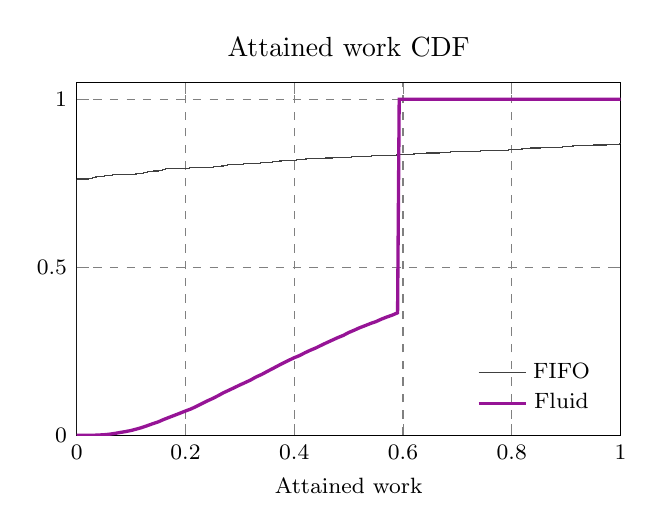
\begin{tikzpicture}
\begin{axis}[
    title=Attained work CDF,
    width=0.7\textwidth,
    height=0.5\textwidth,
    xlabel={Attained work},
    xmin=0,xmax=1.0,
    ymin=0,ymax=1.05,
    grid,
    legend pos=south east,
    ]
    \addplot[color=black!75!white, solid, const plot]
        table[row sep={\\}]
        {
            \\
            0.0  0.0012484394506866417  \\
            0.0  0.0024968789013732834  \\
            0.0  0.003745318352059925  \\
            0.0  0.004993757802746567  \\
            0.0  0.006242197253433208  \\
            0.0  0.00749063670411985  \\
            0.0  0.008739076154806492  \\
            0.0  0.009987515605493134  \\
            0.0  0.011235955056179775  \\
            0.0  0.012484394506866416  \\
            0.0  0.01373283395755306  \\
            0.0  0.0149812734082397  \\
            0.0  0.016229712858926344  \\
            0.0  0.017478152309612985  \\
            0.0  0.018726591760299626  \\
            0.0  0.019975031210986267  \\
            0.0  0.02122347066167291  \\
            0.0  0.02247191011235955  \\
            0.0  0.02372034956304619  \\
            0.0  0.024968789013732832  \\
            0.0  0.026217228464419477  \\
            0.0  0.02746566791510612  \\
            0.0  0.02871410736579276  \\
            0.0  0.0299625468164794  \\
            0.0  0.031210986267166042  \\
            0.0  0.03245942571785269  \\
            0.0  0.033707865168539325  \\
            0.0  0.03495630461922597  \\
            0.0  0.03620474406991261  \\
            0.0  0.03745318352059925  \\
            0.0  0.03870162297128589  \\
            0.0  0.039950062421972535  \\
            0.0  0.04119850187265917  \\
            0.0  0.04244694132334582  \\
            0.0  0.04369538077403246  \\
            0.0  0.0449438202247191  \\
            0.0  0.046192259675405745  \\
            0.0  0.04744069912609238  \\
            0.0  0.04868913857677903  \\
            0.0  0.049937578027465665  \\
            0.0  0.05118601747815231  \\
            0.0  0.052434456928838954  \\
            0.0  0.05368289637952559  \\
            0.0  0.05493133583021224  \\
            0.0  0.056179775280898875  \\
            0.0  0.05742821473158552  \\
            0.0  0.05867665418227216  \\
            0.0  0.0599250936329588  \\
            0.0  0.06117353308364544  \\
            0.0  0.062421972534332085  \\
            0.0  0.06367041198501873  \\
            0.0  0.06491885143570537  \\
            0.0  0.066167290886392  \\
            0.0  0.06741573033707865  \\
            0.0  0.0686641697877653  \\
            0.0  0.06991260923845194  \\
            0.0  0.07116104868913857  \\
            0.0  0.07240948813982521  \\
            0.0  0.07365792759051186  \\
            0.0  0.0749063670411985  \\
            0.0  0.07615480649188515  \\
            0.0  0.07740324594257178  \\
            0.0  0.07865168539325842  \\
            0.0  0.07990012484394507  \\
            0.0  0.08114856429463171  \\
            0.0  0.08239700374531835  \\
            0.0  0.08364544319600499  \\
            0.0  0.08489388264669163  \\
            0.0  0.08614232209737828  \\
            0.0  0.08739076154806492  \\
            0.0  0.08863920099875156  \\
            0.0  0.0898876404494382  \\
            0.0  0.09113607990012484  \\
            0.0  0.09238451935081149  \\
            0.0  0.09363295880149813  \\
            0.0  0.09488139825218476  \\
            0.0  0.09612983770287141  \\
            0.0  0.09737827715355805  \\
            0.0  0.0986267166042447  \\
            0.0  0.09987515605493133  \\
            0.0  0.10112359550561797  \\
            0.0  0.10237203495630462  \\
            0.0  0.10362047440699126  \\
            0.0  0.10486891385767791  \\
            0.0  0.10611735330836454  \\
            0.0  0.10736579275905118  \\
            0.0  0.10861423220973783  \\
            0.0  0.10986267166042447  \\
            0.0  0.1111111111111111  \\
            0.0  0.11235955056179775  \\
            0.0  0.1136079900124844  \\
            0.0  0.11485642946317104  \\
            0.0  0.11610486891385768  \\
            0.0  0.11735330836454431  \\
            0.0  0.11860174781523096  \\
            0.0  0.1198501872659176  \\
            0.0  0.12109862671660425  \\
            0.0  0.12234706616729088  \\
            0.0  0.12359550561797752  \\
            0.0  0.12484394506866417  \\
            0.0  0.12609238451935081  \\
            0.0  0.12734082397003746  \\
            0.0  0.1285892634207241  \\
            0.0  0.12983770287141075  \\
            0.0  0.13108614232209737  \\
            0.0  0.132334581772784  \\
            0.0  0.13358302122347065  \\
            0.0  0.1348314606741573  \\
            0.0  0.13607990012484394  \\
            0.0  0.1373283395755306  \\
            0.0  0.13857677902621723  \\
            0.0  0.13982521847690388  \\
            0.0  0.14107365792759052  \\
            0.0  0.14232209737827714  \\
            0.0  0.14357053682896379  \\
            0.0  0.14481897627965043  \\
            0.0  0.14606741573033707  \\
            0.0  0.14731585518102372  \\
            0.0  0.14856429463171036  \\
            0.0  0.149812734082397  \\
            0.0  0.15106117353308365  \\
            0.0  0.1523096129837703  \\
            0.0  0.15355805243445692  \\
            0.0  0.15480649188514356  \\
            0.0  0.1560549313358302  \\
            0.0  0.15730337078651685  \\
            0.0  0.1585518102372035  \\
            0.0  0.15980024968789014  \\
            0.0  0.16104868913857678  \\
            0.0  0.16229712858926343  \\
            0.0  0.16354556803995007  \\
            0.0  0.1647940074906367  \\
            0.0  0.16604244694132334  \\
            0.0  0.16729088639200998  \\
            0.0  0.16853932584269662  \\
            0.0  0.16978776529338327  \\
            0.0  0.17103620474406991  \\
            0.0  0.17228464419475656  \\
            0.0  0.1735330836454432  \\
            0.0  0.17478152309612985  \\
            0.0  0.1760299625468165  \\
            0.0  0.1772784019975031  \\
            0.0  0.17852684144818975  \\
            0.0  0.1797752808988764  \\
            0.0  0.18102372034956304  \\
            0.0  0.1822721598002497  \\
            0.0  0.18352059925093633  \\
            0.0  0.18476903870162298  \\
            0.0  0.18601747815230962  \\
            0.0  0.18726591760299627  \\
            0.0  0.18851435705368288  \\
            0.0  0.18976279650436953  \\
            0.0  0.19101123595505617  \\
            0.0  0.19225967540574282  \\
            0.0  0.19350811485642946  \\
            0.0  0.1947565543071161  \\
            0.0  0.19600499375780275  \\
            0.0  0.1972534332084894  \\
            0.0  0.19850187265917604  \\
            0.0  0.19975031210986266  \\
            0.0  0.2009987515605493  \\
            0.0  0.20224719101123595  \\
            0.0  0.2034956304619226  \\
            0.0  0.20474406991260924  \\
            0.0  0.20599250936329588  \\
            0.0  0.20724094881398253  \\
            0.0  0.20848938826466917  \\
            0.0  0.20973782771535582  \\
            0.0  0.21098626716604243  \\
            0.0  0.21223470661672908  \\
            0.0  0.21348314606741572  \\
            0.0  0.21473158551810237  \\
            0.0  0.21598002496878901  \\
            0.0  0.21722846441947566  \\
            0.0  0.2184769038701623  \\
            0.0  0.21972534332084895  \\
            0.0  0.2209737827715356  \\
            0.0  0.2222222222222222  \\
            0.0  0.22347066167290885  \\
            0.0  0.2247191011235955  \\
            0.0  0.22596754057428214  \\
            0.0  0.2272159800249688  \\
            0.0  0.22846441947565543  \\
            0.0  0.22971285892634208  \\
            0.0  0.23096129837702872  \\
            0.0  0.23220973782771537  \\
            0.0  0.23345817727840198  \\
            0.0  0.23470661672908863  \\
            0.0  0.23595505617977527  \\
            0.0  0.23720349563046192  \\
            0.0  0.23845193508114856  \\
            0.0  0.2397003745318352  \\
            0.0  0.24094881398252185  \\
            0.0  0.2421972534332085  \\
            0.0  0.24344569288389514  \\
            0.0  0.24469413233458176  \\
            0.0  0.2459425717852684  \\
            0.0  0.24719101123595505  \\
            0.0  0.2484394506866417  \\
            0.0  0.24968789013732834  \\
            0.0  0.250936329588015  \\
            0.0  0.25218476903870163  \\
            0.0  0.2534332084893883  \\
            0.0  0.2546816479400749  \\
            0.0  0.25593008739076156  \\
            0.0  0.2571785268414482  \\
            0.0  0.25842696629213485  \\
            0.0  0.2596754057428215  \\
            0.0  0.26092384519350814  \\
            0.0  0.26217228464419473  \\
            0.0  0.2634207240948814  \\
            0.0  0.264669163545568  \\
            0.0  0.26591760299625467  \\
            0.0  0.2671660424469413  \\
            0.0  0.26841448189762795  \\
            0.0  0.2696629213483146  \\
            0.0  0.27091136079900124  \\
            0.0  0.2721598002496879  \\
            0.0  0.27340823970037453  \\
            0.0  0.2746566791510612  \\
            0.0  0.2759051186017478  \\
            0.0  0.27715355805243447  \\
            0.0  0.2784019975031211  \\
            0.0  0.27965043695380776  \\
            0.0  0.2808988764044944  \\
            0.0  0.28214731585518105  \\
            0.0  0.2833957553058677  \\
            0.0  0.2846441947565543  \\
            0.0  0.2858926342072409  \\
            0.0  0.28714107365792757  \\
            0.0  0.2883895131086142  \\
            0.0  0.28963795255930086  \\
            0.0  0.2908863920099875  \\
            0.0  0.29213483146067415  \\
            0.0  0.2933832709113608  \\
            0.0  0.29463171036204744  \\
            0.0  0.2958801498127341  \\
            0.0  0.29712858926342073  \\
            0.0  0.2983770287141074  \\
            0.0  0.299625468164794  \\
            0.0  0.30087390761548066  \\
            0.0  0.3021223470661673  \\
            0.0  0.30337078651685395  \\
            0.0  0.3046192259675406  \\
            0.0  0.30586766541822724  \\
            0.0  0.30711610486891383  \\
            0.0  0.3083645443196005  \\
            0.0  0.3096129837702871  \\
            0.0  0.31086142322097376  \\
            0.0  0.3121098626716604  \\
            0.0  0.31335830212234705  \\
            0.0  0.3146067415730337  \\
            0.0  0.31585518102372034  \\
            0.0  0.317103620474407  \\
            0.0  0.31835205992509363  \\
            0.0  0.3196004993757803  \\
            0.0  0.3208489388264669  \\
            0.0  0.32209737827715357  \\
            0.0  0.3233458177278402  \\
            0.0  0.32459425717852686  \\
            0.0  0.3258426966292135  \\
            0.0  0.32709113607990015  \\
            0.0  0.3283395755305868  \\
            0.0  0.3295880149812734  \\
            0.0  0.33083645443196  \\
            0.0  0.33208489388264667  \\
            0.0  0.3333333333333333  \\
            0.0  0.33458177278401996  \\
            0.0  0.3358302122347066  \\
            0.0  0.33707865168539325  \\
            0.0  0.3383270911360799  \\
            0.0  0.33957553058676654  \\
            0.0  0.3408239700374532  \\
            0.0  0.34207240948813983  \\
            0.0  0.3433208489388265  \\
            0.0  0.3445692883895131  \\
            0.0  0.34581772784019976  \\
            0.0  0.3470661672908864  \\
            0.0  0.34831460674157305  \\
            0.0  0.3495630461922597  \\
            0.0  0.35081148564294634  \\
            0.0  0.352059925093633  \\
            0.0  0.3533083645443196  \\
            0.0  0.3545568039950062  \\
            0.0  0.35580524344569286  \\
            0.0  0.3570536828963795  \\
            0.0  0.35830212234706615  \\
            0.0  0.3595505617977528  \\
            0.0  0.36079900124843944  \\
            0.0  0.3620474406991261  \\
            0.0  0.36329588014981273  \\
            0.0  0.3645443196004994  \\
            0.0  0.365792759051186  \\
            0.0  0.36704119850187267  \\
            0.0  0.3682896379525593  \\
            0.0  0.36953807740324596  \\
            0.0  0.3707865168539326  \\
            0.0  0.37203495630461925  \\
            0.0  0.3732833957553059  \\
            0.0  0.37453183520599254  \\
            0.0  0.3757802746566791  \\
            0.0  0.37702871410736577  \\
            0.0  0.3782771535580524  \\
            0.0  0.37952559300873906  \\
            0.0  0.3807740324594257  \\
            0.0  0.38202247191011235  \\
            0.0  0.383270911360799  \\
            0.0  0.38451935081148564  \\
            0.0  0.3857677902621723  \\
            0.0  0.38701622971285893  \\
            0.0  0.3882646691635456  \\
            0.0  0.3895131086142322  \\
            0.0  0.39076154806491886  \\
            0.0  0.3920099875156055  \\
            0.0  0.39325842696629215  \\
            0.0  0.3945068664169788  \\
            0.0  0.39575530586766544  \\
            0.0  0.3970037453183521  \\
            0.0  0.3982521847690387  \\
            0.0  0.3995006242197253  \\
            0.0  0.40074906367041196  \\
            0.0  0.4019975031210986  \\
            0.0  0.40324594257178525  \\
            0.0  0.4044943820224719  \\
            0.0  0.40574282147315854  \\
            0.0  0.4069912609238452  \\
            0.0  0.40823970037453183  \\
            0.0  0.4094881398252185  \\
            0.0  0.4107365792759051  \\
            0.0  0.41198501872659177  \\
            0.0  0.4132334581772784  \\
            0.0  0.41448189762796506  \\
            0.0  0.4157303370786517  \\
            0.0  0.41697877652933835  \\
            0.0  0.418227215980025  \\
            0.0  0.41947565543071164  \\
            0.0  0.4207240948813982  \\
            0.0  0.42197253433208487  \\
            0.0  0.4232209737827715  \\
            0.0  0.42446941323345816  \\
            0.0  0.4257178526841448  \\
            0.0  0.42696629213483145  \\
            0.0  0.4282147315855181  \\
            0.0  0.42946317103620474  \\
            0.0  0.4307116104868914  \\
            0.0  0.43196004993757803  \\
            0.0  0.4332084893882647  \\
            0.0  0.4344569288389513  \\
            0.0  0.43570536828963796  \\
            0.0  0.4369538077403246  \\
            0.0  0.43820224719101125  \\
            0.0  0.4394506866416979  \\
            0.0  0.44069912609238454  \\
            0.0  0.4419475655430712  \\
            0.0  0.4431960049937578  \\
            0.0  0.4444444444444444  \\
            0.0  0.44569288389513106  \\
            0.0  0.4469413233458177  \\
            0.0  0.44818976279650435  \\
            0.0  0.449438202247191  \\
            0.0  0.45068664169787764  \\
            0.0  0.4519350811485643  \\
            0.0  0.45318352059925093  \\
            0.0  0.4544319600499376  \\
            0.0  0.4556803995006242  \\
            0.0  0.45692883895131087  \\
            0.0  0.4581772784019975  \\
            0.0  0.45942571785268416  \\
            0.0  0.4606741573033708  \\
            0.0  0.46192259675405745  \\
            0.0  0.4631710362047441  \\
            0.0  0.46441947565543074  \\
            0.0  0.4656679151061174  \\
            0.0  0.46691635455680397  \\
            0.0  0.4681647940074906  \\
            0.0  0.46941323345817726  \\
            0.0  0.4706616729088639  \\
            0.0  0.47191011235955055  \\
            0.0  0.4731585518102372  \\
            0.0  0.47440699126092384  \\
            0.0  0.4756554307116105  \\
            0.0  0.4769038701622971  \\
            0.0  0.4781523096129838  \\
            0.0  0.4794007490636704  \\
            0.0  0.48064918851435706  \\
            0.0  0.4818976279650437  \\
            0.0  0.48314606741573035  \\
            0.0  0.484394506866417  \\
            0.0  0.48564294631710364  \\
            0.0  0.4868913857677903  \\
            0.0  0.48813982521847693  \\
            0.0  0.4893882646691635  \\
            0.0  0.49063670411985016  \\
            0.0  0.4918851435705368  \\
            0.0  0.49313358302122345  \\
            0.0  0.4943820224719101  \\
            0.0  0.49563046192259674  \\
            0.0  0.4968789013732834  \\
            0.0  0.49812734082397003  \\
            0.0  0.4993757802746567  \\
            0.0  0.5006242197253433  \\
            0.0  0.50187265917603  \\
            0.0  0.5031210986267166  \\
            0.0  0.5043695380774033  \\
            0.0  0.5056179775280899  \\
            0.0  0.5068664169787765  \\
            0.0  0.5081148564294632  \\
            0.0  0.5093632958801498  \\
            0.0  0.5106117353308365  \\
            0.0  0.5118601747815231  \\
            0.0  0.5131086142322098  \\
            0.0  0.5143570536828964  \\
            0.0  0.5156054931335831  \\
            0.0  0.5168539325842697  \\
            0.0  0.5181023720349563  \\
            0.0  0.519350811485643  \\
            0.0  0.5205992509363296  \\
            0.0  0.5218476903870163  \\
            0.0  0.5230961298377028  \\
            0.0  0.5243445692883895  \\
            0.0  0.5255930087390761  \\
            0.0  0.5268414481897628  \\
            0.0  0.5280898876404494  \\
            0.0  0.529338327091136  \\
            0.0  0.5305867665418227  \\
            0.0  0.5318352059925093  \\
            0.0  0.533083645443196  \\
            0.0  0.5343320848938826  \\
            0.0  0.5355805243445693  \\
            0.0  0.5368289637952559  \\
            0.0  0.5380774032459426  \\
            0.0  0.5393258426966292  \\
            0.0  0.5405742821473158  \\
            0.0  0.5418227215980025  \\
            0.0  0.5430711610486891  \\
            0.0  0.5443196004993758  \\
            0.0  0.5455680399500624  \\
            0.0  0.5468164794007491  \\
            0.0  0.5480649188514357  \\
            0.0  0.5493133583021224  \\
            0.0  0.550561797752809  \\
            0.0  0.5518102372034956  \\
            0.0  0.5530586766541823  \\
            0.0  0.5543071161048689  \\
            0.0  0.5555555555555556  \\
            0.0  0.5568039950062422  \\
            0.0  0.5580524344569289  \\
            0.0  0.5593008739076155  \\
            0.0  0.5605493133583022  \\
            0.0  0.5617977528089888  \\
            0.0  0.5630461922596754  \\
            0.0  0.5642946317103621  \\
            0.0  0.5655430711610487  \\
            0.0  0.5667915106117354  \\
            0.0  0.568039950062422  \\
            0.0  0.5692883895131086  \\
            0.0  0.5705368289637952  \\
            0.0  0.5717852684144819  \\
            0.0  0.5730337078651685  \\
            0.0  0.5742821473158551  \\
            0.0  0.5755305867665418  \\
            0.0  0.5767790262172284  \\
            0.0  0.5780274656679151  \\
            0.0  0.5792759051186017  \\
            0.0  0.5805243445692884  \\
            0.0  0.581772784019975  \\
            0.0  0.5830212234706617  \\
            0.0  0.5842696629213483  \\
            0.0  0.5855181023720349  \\
            0.0  0.5867665418227216  \\
            0.0  0.5880149812734082  \\
            0.0  0.5892634207240949  \\
            0.0  0.5905118601747815  \\
            0.0  0.5917602996254682  \\
            0.0  0.5930087390761548  \\
            0.0  0.5942571785268415  \\
            0.0  0.5955056179775281  \\
            0.0  0.5967540574282147  \\
            0.0  0.5980024968789014  \\
            0.0  0.599250936329588  \\
            0.0  0.6004993757802747  \\
            0.0  0.6017478152309613  \\
            0.0  0.602996254681648  \\
            0.0  0.6042446941323346  \\
            0.0  0.6054931335830213  \\
            0.0  0.6067415730337079  \\
            0.0  0.6079900124843945  \\
            0.0  0.6092384519350812  \\
            0.0  0.6104868913857678  \\
            0.0  0.6117353308364545  \\
            0.0  0.6129837702871411  \\
            0.0  0.6142322097378277  \\
            0.0  0.6154806491885143  \\
            0.0  0.616729088639201  \\
            0.0  0.6179775280898876  \\
            0.0  0.6192259675405742  \\
            0.0  0.6204744069912609  \\
            0.0  0.6217228464419475  \\
            0.0  0.6229712858926342  \\
            0.0  0.6242197253433208  \\
            0.0  0.6254681647940075  \\
            0.0  0.6267166042446941  \\
            0.0  0.6279650436953808  \\
            0.0  0.6292134831460674  \\
            0.0  0.630461922596754  \\
            0.0  0.6317103620474407  \\
            0.0  0.6329588014981273  \\
            0.0  0.634207240948814  \\
            0.0  0.6354556803995006  \\
            0.0  0.6367041198501873  \\
            0.0  0.6379525593008739  \\
            0.0  0.6392009987515606  \\
            0.0  0.6404494382022472  \\
            0.0  0.6416978776529338  \\
            0.0  0.6429463171036205  \\
            0.0  0.6441947565543071  \\
            0.0  0.6454431960049938  \\
            0.0  0.6466916354556804  \\
            0.0  0.6479400749063671  \\
            0.0  0.6491885143570537  \\
            0.0  0.6504369538077404  \\
            0.0  0.651685393258427  \\
            0.0  0.6529338327091136  \\
            0.0  0.6541822721598003  \\
            0.0  0.6554307116104869  \\
            0.0  0.6566791510611736  \\
            0.0  0.6579275905118602  \\
            0.0  0.6591760299625468  \\
            0.0  0.6604244694132334  \\
            0.0  0.66167290886392  \\
            0.0  0.6629213483146067  \\
            0.0  0.6641697877652933  \\
            0.0  0.66541822721598  \\
            0.0  0.6666666666666666  \\
            0.0  0.6679151061173533  \\
            0.0  0.6691635455680399  \\
            0.0  0.6704119850187266  \\
            0.0  0.6716604244694132  \\
            0.0  0.6729088639200999  \\
            0.0  0.6741573033707865  \\
            0.0  0.6754057428214731  \\
            0.0  0.6766541822721598  \\
            0.0  0.6779026217228464  \\
            0.0  0.6791510611735331  \\
            0.0  0.6803995006242197  \\
            0.0  0.6816479400749064  \\
            0.0  0.682896379525593  \\
            0.0  0.6841448189762797  \\
            0.0  0.6853932584269663  \\
            0.0  0.686641697877653  \\
            0.0  0.6878901373283396  \\
            0.0  0.6891385767790262  \\
            0.0  0.6903870162297129  \\
            0.0  0.6916354556803995  \\
            0.0  0.6928838951310862  \\
            0.0  0.6941323345817728  \\
            0.0  0.6953807740324595  \\
            0.0  0.6966292134831461  \\
            0.0  0.6978776529338327  \\
            0.0  0.6991260923845194  \\
            0.0  0.700374531835206  \\
            0.0  0.7016229712858927  \\
            0.0  0.7028714107365793  \\
            0.0  0.704119850187266  \\
            0.0  0.7053682896379525  \\
            0.0  0.7066167290886392  \\
            0.0  0.7078651685393258  \\
            0.0  0.7091136079900124  \\
            0.0  0.7103620474406991  \\
            0.0  0.7116104868913857  \\
            0.0  0.7128589263420724  \\
            0.0  0.714107365792759  \\
            0.0  0.7153558052434457  \\
            0.0  0.7166042446941323  \\
            0.0  0.717852684144819  \\
            0.0  0.7191011235955056  \\
            0.0  0.7203495630461922  \\
            0.0  0.7215980024968789  \\
            0.0  0.7228464419475655  \\
            0.0  0.7240948813982522  \\
            0.0  0.7253433208489388  \\
            0.0  0.7265917602996255  \\
            0.0  0.7278401997503121  \\
            0.0  0.7290886392009988  \\
            0.0  0.7303370786516854  \\
            0.0  0.731585518102372  \\
            0.0  0.7328339575530587  \\
            0.0  0.7340823970037453  \\
            0.0  0.735330836454432  \\
            0.0  0.7365792759051186  \\
            0.0  0.7378277153558053  \\
            0.0  0.7390761548064919  \\
            0.0  0.7403245942571786  \\
            0.0  0.7415730337078652  \\
            0.0  0.7428214731585518  \\
            0.0  0.7440699126092385  \\
            0.0  0.7453183520599251  \\
            0.0  0.7465667915106118  \\
            0.0  0.7478152309612984  \\
            0.0  0.7490636704119851  \\
            0.0  0.7503121098626716  \\
            0.0  0.7515605493133583  \\
            0.0  0.7528089887640449  \\
            0.0  0.7540574282147315  \\
            0.0  0.7553058676654182  \\
            0.0  0.7565543071161048  \\
            0.0  0.7578027465667915  \\
            0.0  0.7590511860174781  \\
            0.0  0.7602996254681648  \\
            0.0  0.7615480649188514  \\
            0.0007753404385368867  0.762796504369538  \\
            0.02065745307521638  0.7640449438202247  \\
            0.022833969340808835  0.7652933832709113  \\
            0.028983568673844218  0.766541822721598  \\
            0.03161008050015113  0.7677902621722846  \\
            0.035404145378613805  0.7690387016229713  \\
            0.03647020942396928  0.7702871410736579  \\
            0.04208065785125825  0.7715355805243446  \\
            0.05178212771039625  0.7727840199750312  \\
            0.05765667547940723  0.7740324594257179  \\
            0.06549295478532358  0.7752808988764045  \\
            0.08204273877481683  0.7765293383270911  \\
            0.1088875433878016  0.7777777777777778  \\
            0.11069253470780893  0.7790262172284644  \\
            0.11403673619504673  0.7802746566791511  \\
            0.12286497978559652  0.7815230961298377  \\
            0.1270344511226753  0.7827715355805244  \\
            0.1305140343082627  0.784019975031211  \\
            0.13999727780328186  0.7852684144818977  \\
            0.1405678401055539  0.7865168539325843  \\
            0.1495676641041399  0.787765293383271  \\
            0.15364671116876139  0.7890137328339576  \\
            0.15771446526127875  0.7902621722846442  \\
            0.16060527593550944  0.7915106117353309  \\
            0.16332699475445622  0.7927590511860175  \\
            0.1877460543600762  0.7940074906367042  \\
            0.1966272297126892  0.7952559300873908  \\
            0.20803254185024755  0.7965043695380774  \\
            0.21378519033988397  0.797752808988764  \\
            0.25161990329586104  0.7990012484394506  \\
            0.2659336663535399  0.8002496878901373  \\
            0.26670210020613894  0.8014981273408239  \\
            0.2706648271070762  0.8027465667915106  \\
            0.2739652901445808  0.8039950062421972  \\
            0.2774891590947397  0.8052434456928839  \\
            0.2855454622696101  0.8064918851435705  \\
            0.3074745455446717  0.8077403245942572  \\
            0.309035752680046  0.8089887640449438  \\
            0.3304558148568475  0.8102372034956304  \\
            0.33786244090611817  0.8114856429463171  \\
            0.3432453044588506  0.8127340823970037  \\
            0.3602111591221515  0.8139825218476904  \\
            0.36473123974623967  0.815230961298377  \\
            0.3732512499169829  0.8164794007490637  \\
            0.3759984458196204  0.8177278401997503  \\
            0.4016011471900498  0.818976279650437  \\
            0.40341183969597694  0.8202247191011236  \\
            0.4170346991637359  0.8214731585518102  \\
            0.4216789301951849  0.8227215980024969  \\
            0.43719678384164595  0.8239700374531835  \\
            0.45756626464588024  0.8252184769038702  \\
            0.46986466230243806  0.8264669163545568  \\
            0.48593186018562307  0.8277153558052435  \\
            0.5054021420644403  0.8289637952559301  \\
            0.5363770912320831  0.8302122347066168  \\
            0.5422749518049201  0.8314606741573034  \\
            0.5827082973175948  0.83270911360799  \\
            0.5859198642705792  0.8339575530586767  \\
            0.5888311727662341  0.8352059925093633  \\
            0.5991281034352269  0.83645443196005  \\
            0.6201905507272869  0.8377028714107366  \\
            0.635709519429966  0.8389513108614233  \\
            0.6440929279658789  0.8401997503121099  \\
            0.6664343310597189  0.8414481897627965  \\
            0.674305978358035  0.8426966292134831  \\
            0.6875209988559661  0.8439450686641697  \\
            0.6932599951169749  0.8451935081148564  \\
            0.7419823710186932  0.846441947565543  \\
            0.755537033918408  0.8476903870162297  \\
            0.7613137956237992  0.8489388264669163  \\
            0.7944213030767138  0.850187265917603  \\
            0.8065932734878984  0.8514357053682896  \\
            0.8189086179528566  0.8526841448189763  \\
            0.832419726857168  0.8539325842696629  \\
            0.8348135637254579  0.8551810237203495  \\
            0.8524891699511841  0.8564294631710362  \\
            0.8758456734141546  0.8576779026217228  \\
            0.8931532027986937  0.8589263420724095  \\
            0.9101706258738211  0.8601747815230961  \\
            0.9126296234244009  0.8614232209737828  \\
            0.9229884274028279  0.8626716604244694  \\
            0.9502086859711483  0.8639200998751561  \\
            0.9749802977458586  0.8651685393258427  \\
            0.9965682707490231  0.8664169787765293  \\
            0.997503228334363  0.867665418227216  \\
            1.00892639258592  0.8689138576779026  \\
            1.0132539701107248  0.8701622971285893  \\
            1.0208579738714647  0.8714107365792759  \\
            1.0241454491218036  0.8726591760299626  \\
            1.0386418544039913  0.8739076154806492  \\
            1.051012267978912  0.8751560549313359  \\
            1.072788343242518  0.8764044943820225  \\
            1.0801489925855137  0.8776529338327091  \\
            1.0953251431002333  0.8789013732833958  \\
            1.1321277110903551  0.8801498127340824  \\
            1.1391524968314286  0.8813982521847691  \\
            1.153427224171708  0.8826466916354557  \\
            1.1562497640441123  0.8838951310861424  \\
            1.1674183555531665  0.885143570536829  \\
            1.2307132142135444  0.8863920099875156  \\
            1.3239484440909006  0.8876404494382022  \\
            1.3506841447857738  0.8888888888888888  \\
            1.3533116290317793  0.8901373283395755  \\
            1.3685209216435648  0.8913857677902621  \\
            1.3808675697044634  0.8926342072409488  \\
            1.426322347258881  0.8938826466916354  \\
            1.4305230897723362  0.8951310861423221  \\
            1.4419802236019024  0.8963795255930087  \\
            1.4739735735238852  0.8976279650436954  \\
            1.4768542310729487  0.898876404494382  \\
            1.4920218728104062  0.9001248439450686  \\
            1.495190874928948  0.9013732833957553  \\
            1.5066554263171668  0.9026217228464419  \\
            1.511993310928755  0.9038701622971286  \\
            1.5575309031839737  0.9051186017478152  \\
            1.5807725566640514  0.9063670411985019  \\
            1.6136827265958402  0.9076154806491885  \\
            1.6861383057220678  0.9088639200998752  \\
            1.6868888149081709  0.9101123595505618  \\
            1.7089077456319322  0.9113607990012484  \\
            1.751631096195892  0.9126092384519351  \\
            1.758119691760733  0.9138576779026217  \\
            1.773984330326953  0.9151061173533084  \\
            1.8418374841727996  0.916354556803995  \\
            1.8436376104656063  0.9176029962546817  \\
            1.870893593551254  0.9188514357053683  \\
            1.9295829612358553  0.920099875156055  \\
            1.9718241965908025  0.9213483146067416  \\
            1.9815933730950235  0.9225967540574282  \\
            2.0089523254909523  0.9238451935081149  \\
            2.0628325074833196  0.9250936329588015  \\
            2.0679906330215196  0.9263420724094882  \\
            2.083958428345838  0.9275905118601748  \\
            2.098231902042045  0.9288389513108615  \\
            2.171168747871712  0.9300873907615481  \\
            2.174101629223643  0.9313358302122348  \\
            2.1873142757102784  0.9325842696629213  \\
            2.2094450745660748  0.9338327091136079  \\
            2.2151427964900634  0.9350811485642946  \\
            2.2472361778734804  0.9363295880149812  \\
            2.2542845841308488  0.9375780274656679  \\
            2.292632460660215  0.9388264669163545  \\
            2.303389430246355  0.9400749063670412  \\
            2.311532530807897  0.9413233458177278  \\
            2.328380695577465  0.9425717852684145  \\
            2.331720062990101  0.9438202247191011  \\
            2.4783836174710743  0.9450686641697877  \\
            2.4947280245145578  0.9463171036204744  \\
            2.691714580462334  0.947565543071161  \\
            2.7096480734611514  0.9488139825218477  \\
            2.802067576599588  0.9500624219725343  \\
            2.815369357577275  0.951310861423221  \\
            2.946827608454022  0.9525593008739076  \\
            3.1215019727249995  0.9538077403245943  \\
            3.1277340059858822  0.9550561797752809  \\
            3.171483639006869  0.9563046192259675  \\
            3.173924162242379  0.9575530586766542  \\
            3.219614380143084  0.9588014981273408  \\
            3.2383910609824405  0.9600499375780275  \\
            3.2569460760361446  0.9612983770287141  \\
            3.310777807062335  0.9625468164794008  \\
            3.3519523510504214  0.9637952559300874  \\
            3.3618027766832657  0.9650436953807741  \\
            3.41045712535497  0.9662921348314607  \\
            3.4343790939098113  0.9675405742821473  \\
            3.4939148701192813  0.968789013732834  \\
            3.546199420589275  0.9700374531835206  \\
            3.6079471778067536  0.9712858926342073  \\
            3.7554903874820726  0.9725343320848939  \\
            3.9382468466631027  0.9737827715355806  \\
            3.9718875782308523  0.9750312109862672  \\
            4.0442246166693785  0.9762796504369539  \\
            4.152073750515958  0.9775280898876404  \\
            4.174193576993716  0.978776529338327  \\
            4.4886619198083615  0.9800249687890137  \\
            4.593544951016188  0.9812734082397003  \\
            4.7534713802452835  0.982521847690387  \\
            4.824159045755658  0.9837702871410736  \\
            5.066992346210604  0.9850187265917603  \\
            5.562602066787861  0.9862671660424469  \\
            5.574946452247003  0.9875156054931336  \\
            5.7432846758013625  0.9887640449438202  \\
            5.7649839588404515  0.9900124843945068  \\
            7.213060868827269  0.9912609238451935  \\
            7.894655141175377  0.9925093632958801  \\
            7.965206667227582  0.9937578027465668  \\
            8.030023248388844  0.9950062421972534  \\
            8.36852199571929  0.9962546816479401  \\
            9.171172598791632  0.9975031210986267  \\
            9.971100195800169  0.9987515605493134  \\
            22.0192523574665  1.0  \\
        }
        ;
    \addlegendentry {FIFO}
    \addplot[color=violetita,solid, very thick]
        table[row sep={\\}]
        {
            \\
            0.0  0.0  \\
            0.01  0.0  \\
            0.02  5.0e-5  \\
            0.03  0.00025  \\
            0.04  0.0009  \\
            0.05  0.0018  \\
            0.06  0.0033  \\
            0.07  0.00575  \\
            0.08  0.00855  \\
            0.09  0.0113  \\
            0.1  0.01445  \\
            0.11  0.01875  \\
            0.12  0.0233  \\
            0.13  0.02895  \\
            0.14  0.0347  \\
            0.15  0.0402  \\
            0.16  0.0472  \\
            0.17  0.05355  \\
            0.18  0.0597  \\
            0.19  0.066  \\
            0.2  0.07245  \\
            0.21  0.07855  \\
            0.22  0.08605  \\
            0.23  0.09415  \\
            0.24  0.1024  \\
            0.25  0.1097  \\
            0.26  0.118  \\
            0.27  0.1269  \\
            0.28  0.1344  \\
            0.29  0.14205  \\
            0.3  0.1499  \\
            0.31  0.1572  \\
            0.32  0.16485  \\
            0.33  0.17395  \\
            0.34  0.18115  \\
            0.35  0.1899  \\
            0.36  0.19835  \\
            0.37  0.20695  \\
            0.38  0.2154  \\
            0.39  0.22335  \\
            0.4  0.231  \\
            0.41  0.2376  \\
            0.42  0.24605  \\
            0.43  0.25355  \\
            0.44  0.2603  \\
            0.45  0.2683  \\
            0.46  0.276  \\
            0.47  0.2834  \\
            0.48  0.29075  \\
            0.49  0.29725  \\
            0.5  0.30585  \\
            0.51  0.31265  \\
            0.52  0.32005  \\
            0.53  0.3262  \\
            0.54  0.3327  \\
            0.55  0.33825  \\
            0.56  0.3456  \\
            0.57  0.352  \\
            0.58  0.3576  \\
            0.59  0.36465  \\
            0.593  1.0  \\
            1.0  1.0  \\
        }
        ;
    \addlegendentry {Fluid}
\end{axis}
\end{tikzpicture}

	\end{center}

	\vfill

	Almost 80\% of the jobs leave without service.
\end{frame}

\section{Final remarks}

\begin{frame}{Messages from the talk}
	
	\begin{myitem}
		\item Measure-valued processes are a powerful tool to model general service queues.
		\item Partial service queues require two-dimensional measures.
		\item Our proposed dynamics for fluid models are tractable and approximate the real system.
		\item Last-but-not-least: in this setting, \alert{deadline-oblivious} policies can be used without performance penalty!
	\end{myitem}
\end{frame}

\begin{frame}{Future work}
	
	\begin{myitem}
		\item Analyze further policies using these tools (FCFS is easy for instance).
		\item Establish process-level convergence to the fluid models (long work...help needed...)
		\item Devise new policies and/or analyze different settings:
		
		\begin{itemize}
			\item Tasks stay until service completion, but we want to measure the average \emph{tardiness}, i.e. how late they depart.
		\end{itemize}
	\end{myitem}
\end{frame}


\begin{frame}[plain]
	\vfill
	{\Huge \alert{Gracias!}}
	\vfill
	Andres Ferragut

	\smallskip

	\href{mailto://ferragut@ort.edu.uy}{\alert{ferragut@ort.edu.uy}}
	
	\smallskip

	\href{http://aferragu.github.io}{\alert{https://aferragu.github.io}}
\end{frame}

\begin{frame}[allowframebreaks]{References}
	\bibliography{reneging}
\end{frame}
\end{document}
